\newcommand{\mydriver}{pdftex} %Making a PDF directly using pdflatex.

\documentclass[12pt,\mydriver]{thesis}  %12pt is larger than 11pt

\usepackage{titlesec}
   \titleformat{\chapter}
      {\normalfont\large}{Chapter \thechapter:}{1em}{}
\usepackage{setspace}
\usepackage{graphicx}
\usepackage{cite}
\usepackage{lscape}
\usepackage{indentfirst}
\usepackage{latexsym}
\usepackage{multirow}
\usepackage{wrapfig}
\usepackage{slashbox}
\usepackage{longtable}
\usepackage{booktabs}
\usepackage{supertabular}
\usepackage{subfigure}
\usepackage[version=4]{mhchem}
\usepackage[bookmarks, colorlinks=true, plainpages=false, citecolor=blue, urlcolor=blue, filecolor=blue, linkcolor=blue]{hyperref} 
\usepackage{tabularx}
	%Works with PcTex.  You may have to choose one of the drivers above if dvips does not work.
\usepackage{zref}		% allows cross referencing between files
\usepackage{cprotect} 	% allows for \verb in table captions
\usepackage{rotating}
\usepackage{placeins}

\newenvironment{figurehere}
  {\def\@captype{figure}}
  {\par\vspace{3em}}% or \par\vspace{1ex} etc.

\newcommand{\tbsp}{\rule{0pt}{18pt}} %used to get a vertical distance after \hline
\setlength{\textwidth}{5.9in}
\setlength{\textheight}{9in}
\setlength{\topmargin}{-.50in}
\setlength{\oddsidemargin}{.55in}
\setlength{\parindent}{.4in}
\pagestyle{empty}

\begin{document}
%Abstract Page 

\hbox{\ }

\renewcommand{\baselinestretch}{1}
\small \normalsize

\begin{center}
\large{{ABSTRACT}} 

\vspace{3em} 

\end{center}
\hspace{-.15in}
\begin{tabular}{ll}
Title of thesis:		& {\large  ANALYSIS OF PROPANE GAS FIRE}	\\
							& {\large  EXPERIMENTS AND SIMULATIONS} 	\\
							& {\large  IN RESIDENTIAL SCALE STRUCTURES} \\
\ \\
							& {\large  Joseph M. Willi, Master of Science, 2017} \\
\ \\
Thesis directed by: 	& {\large  Professor James A. Milke} \\
							& {\large  Department of Fire Protection Engineering} \\
\end{tabular}

\vspace{3em}

\renewcommand{\baselinestretch}{2}
\large \normalsize

Nine full-scale fire experiments were conducted in two residential-sized structures with a fire source provided by three propane gas burners. Five of the experiments were conducted in a single-story structure, and four were conducted in a two-story structure. The structures were instrumented to measure temperature; oxygen and carbon dioxide gas concentrations; gas velocity; and heat flux. Various doors and vents were opened and closed during the experiments to change the ventilation through the structures. Numerical simulations of the nine experiments were conducted using Fire Dynamics Simulator (FDS) (version 6.5.3). The model data  were compared to the corresponding experimental data, and the temperature, gas species concentration, and heat flux data produced by the simulations were within the expected agreement range based on the values of experimental relative standard deviation, model relative standard deviation, and model bias factor provided by the FDS Validation Guide for each specific data type. The one significant discrepancy between the simulation data and experimental data occurred with the gas velocity measurements, which produced a model relative standard deviation that was 0.18 larger than the value from the FDS Validation Guide. Overall, comparing the FDS simulation output to the experimental data shows sufficient agreement between the predicted and measured data, thus indicating that FDS is capable of accurately modeling different aspects of fire scenarios in residential-sized structures.

% However, if the average gas velocity across the entire vent was to be considered instead of individual point measurements, the uncertainty is only 0.05 greater than the values presented in the guide.

 %(must be first, required, non-numbered)
%Titlepage

\thispagestyle{empty}
\hbox{\ }
\vspace{1in}
\renewcommand{\baselinestretch}{1}
\small\normalsize
\begin{center}

\large{{Analysis of Propane Gas Fire Experiments and Simulations in Residential Scale Structures}}\\
\ \\
\ \\
\large{by} \\
\ \\
\large{Joseph Martin Willi}%Your full name as it appears in University records.
\ \\
\ \\
\ \\
\ \\
\normalsize
Thesis submitted to the Faculty of the Graduate School of the \\
University of Maryland, College Park in partial fulfillment \\
of the requirements for the degree of \\
Master of Science \\
2017
\end{center}

\vspace{7.5em}

\noindent Advisory Committee: \\
Professor James A. Milke, Chair \\
Professor Arnaud Trouv\'e \\
Dr. Craig Weinschenk
 %(must follow Abstract, required, non-numbered)
%Copyright

\thispagestyle{empty}
\hbox{\ }

\vfill
\renewcommand{\baselinestretch}{1}
\small\normalsize

\vspace{-.65in}

\begin{center}
\large{\copyright \hbox{ }Copyright by\\
Joseph Martin Willi  %Type your name as it appears in University records
\\
2017}
\end{center}

\vfill
 %(highly recommended, non-numbered)

%Pages from this point start at lower-case Roman number ii)
\pagestyle{plain}
\pagenumbering{roman}
\setcounter{page}{2}

% \include{Preface}  %(if present, start at lower-case Roman number ii)
% \include{Foreword} %(if present, lower-case Roman)
% \include{Dedication} %(if present, lower-case Roman)
%Acknowledgments

\renewcommand{\baselinestretch}{2}
\small\normalsize
\hbox{\ }
 
\vspace{-.65in}

\begin{center}
\large{Acknowledgments} 
\end{center} 

\vspace{1ex}

[PLACEHOLDER]

% NIST, Milke, family, Kevin, people on committee 

% The author would like to thank Daniel Madrzykowski, Roy McLane, Kristopher Overholt, Keith Stakes, and Craig Weinschenk for their contributions in preparing and conducting these experiments.

 %(if present, lower-case Roman)

\setstretch{1}
\tableofcontents %(required, lower-case Roman)
\newpage
\listoftables %(if present, lower-case Roman)
\newpage
\listoffigures %(if present, lower-case Roman)
\newpage
% LIST OF ABBREVIATIONS
\addcontentsline{toc}{chapter}{List of Abbreviations}
%List of Abbreviations

\renewcommand{\baselinestretch}{1}
\small\normalsize
\hbox{\ }

\vspace{-3em}


\begin{center}
\large{List of Abbreviations}
\end{center} 

\vspace{3pt}

\begin{tabular}{ll}
CFD & Computational Fluid Dynamics  \\
FDS & Fire Dynamics Simulator \\
NIST & National Institute of Standards and Technology \\
% PPA & Positive Pressure Attack \\
% PPV & Positive Pressure Ventilation \\
OSB & Oriented Strand Board \\
TJI & Truss Joist I-beams \\
% UL FSRI & Underwriters Laboratories Firefighter Safety Research Institute \\
\end{tabular}


\newpage
\setlength{\parskip}{0em}
\setstretch{2}

%Pages from this point start at Arabic numeral 1
\setcounter{page}{1}
\pagenumbering{arabic}
%%%%%%%%%%%%%%%%%%%%%%%%%%%
% CHAPTER 1: Introduction %
%%%%%%%%%%%%%%%%%%%%%%%%%%%

\renewcommand{\thechapter}{1}

\chapter{Introduction}
The development and behavior of compartment fires, such as those inside residential structures, depend greatly on the ventilation conditions within the compartment. Nine full-scale fire experiments were conducted in residential-sized structures to study how opening and closing different doors and vents affect ventilation and the fire environment. Two experimental structures designed to replicate a single-story and a two-story dwelling were used. The fire source for each experiment was provided by three gas propane burners. The flow of propane to the burners was controlled by a high-precision turn valve and the total displaced gas volume was measured using a rotary gas meter. Local measurements of temperature, gas species concentration, gas velocity, and total heat flux at various locations throughout the structure were collected while the ventilation within the structure was varied through the opening and closing of doors and vents. The nine gas burner experiments were conducted in series with a variety of other experiments, and their original test names were used during the analysis. So, the nine experiments are referred to as Tests~2--6 and Tests~22--25 throughout this report.

Numerical simulations of the nine tests were performed using the program Fire Dynamics Simulator (FDS) (version 6.5.3)~\cite{FDS_Users_Guide}. FDS is a computational fluid dynamics (CFD) code designed to model of thermally-driven fluid flow that is developed and maintained by the National Institute of Standards and Technology (NIST). FDS numerically solves a form of the Navier-Stokes equations for low-speed ($Ma < 0.3$), thermally-driven flows with an emphasis on smoke and heat transport from fires. The FDS Technical Reference Guide~\cite{FDS_Tech_Guide} provides a complete description of the model, including the formulation of the equations and numerical algorithm utilized by the software. 

FDS is mathematically verified~\cite{FDS_Verification_Guide} and validated against a continually growing database of experimental data from a variety of fire scenarios~\cite{FDS_Validation_Guide}. Verification, as defined by the FDS developers, refers to the process of checking the correctness of the solution of governing equations; it checks that the equations are being solved correctly. Validation is the process of determining the appropriateness of the governing equations as a mathematical model of the physical phenomena of interest. Validation typically involves comparing model results with experimental measurements.   

Fire protection engineers commonly use CFD models to predict fire dynamics and smoke movement for potential fire scenarios as they are developing certain fire safety designs. FDS is the most commonly used program for this type of application. Therefore, it's crucial that the program is validated for a range of fire scenarios, including those within residential structures. Currently, there are approximately four different experimental series for which FDS has been validated that involve fires within residential-sized structures containing multiple compartments~\cite{FDS_Validation_Guide}. Furthermore, there are no cases described within the FDS Validation Guide that involve fire scenarios inside multi-story residential scale structures. Thus, generating FDS simulations of the nine gas burner experiments and comparing the results to the experimental data will provide an important addition to the FDS validation database.

This report contains a thorough description of the experimental structures and instrumentation used to collect data during the experiments. The procedures followed during each test are also outlined. Following the description of the experimental setup and procedures, the FDS input files that define experiment simulations are discussed in detail. Next, the data output by the models are compared to the corresponding sensor data of temperature; oxygen and carbon dioxide concentration; gas velocity; and heat flux. Figures of simulation data and experimental data plotted over the duration of the tests are presented alongside log/log scatter plots that summarize the overall results for each data type. The relative standard deviation values for the model and experimental data and the resulting model bias factor are reported with each summary plot. Then, the relative standard deviation values and model bias factor for each data type are compared to the corresponding values listed within the FDS Validation Guide. 
%%%%%%%%%%%%%%%%%%%%%%%%%%%%%%%%%
% CHAPTER 2: Experimental Setup %
%%%%%%%%%%%%%%%%%%%%%%%%%%%%%%%%%

\renewcommand{\thechapter}{2}

\chapter{Experimental Setup}
\label{chap:exp_setup}
The series of field experiments described in this report were conducted in two structures of similar design located at the Delaware County Emergency Services Training Center in Sharon Hill, Pennsylvania. Three propane burners were used as the fire source for all experiments, and the structures were instrumented with various sensors to collect gas temperature, gas velocity, total heat flux, and gas species concentration measurements.

\section{Test Structures}
% The following sections contain detailed information about the construction of each experimental structure and the layout of the structures 

\subsection{Construction}
Each test structure was built on a concrete slab as shown in Figure~\ref{fig:struct_pics}. The East Structure and West Structure were designed to simulate a single-story and two-story residential structure, respectively.

\subsubsection*{\textit{First Floor of Both Structures}}
The first floor of each structure had outer walls composed of interlocking concrete blocks measuring 0.6~m (2.0~ft) wide, 0.6~m (2.0~ft) high, and 1.2~m (4.0~ft) long. The joints and gaps between the blocks were filled with high temperature insulation. All doors along the outer walls were composed of steel.

\begin{figure}
	\centering
	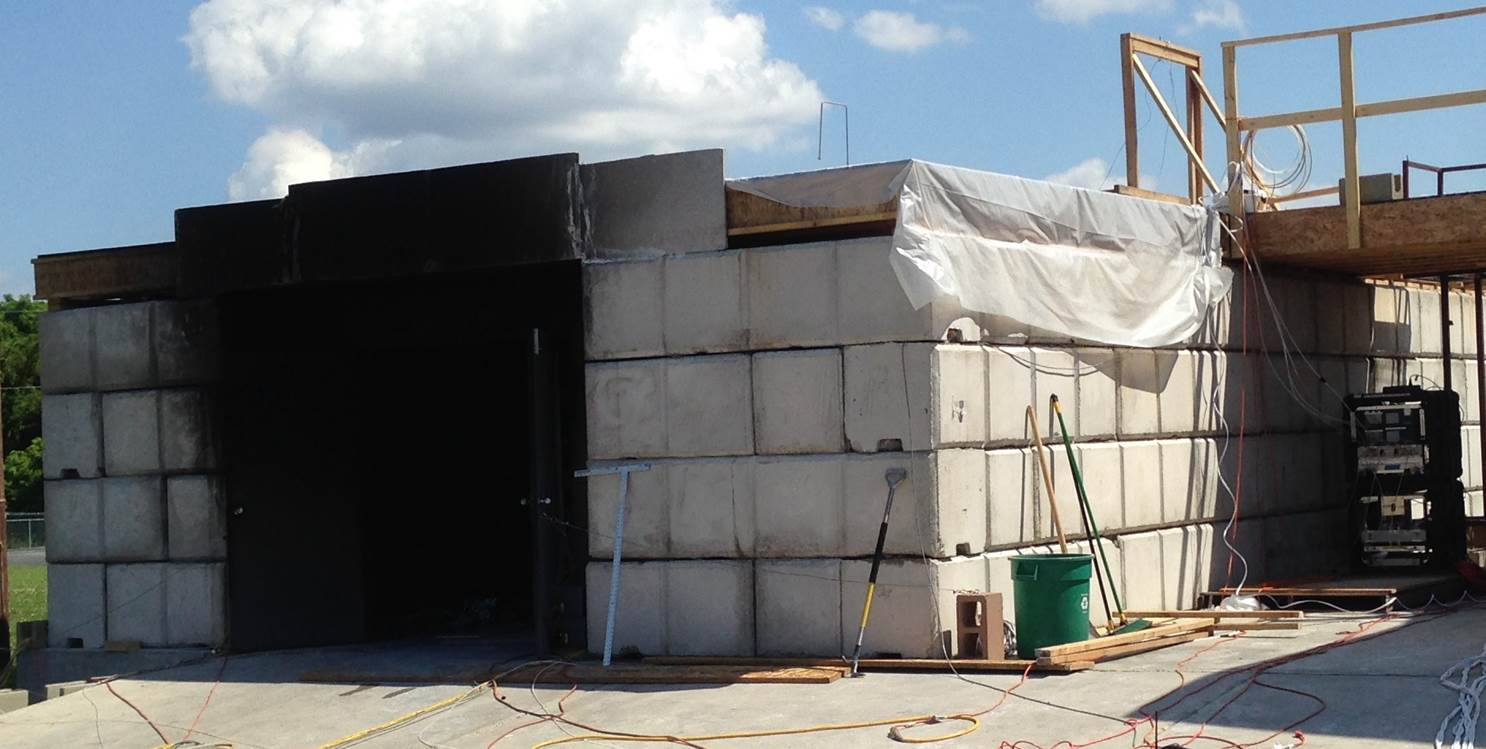
\includegraphics[width=5.25in]{Figures/Pictures/east_structure}
	\\~\\
	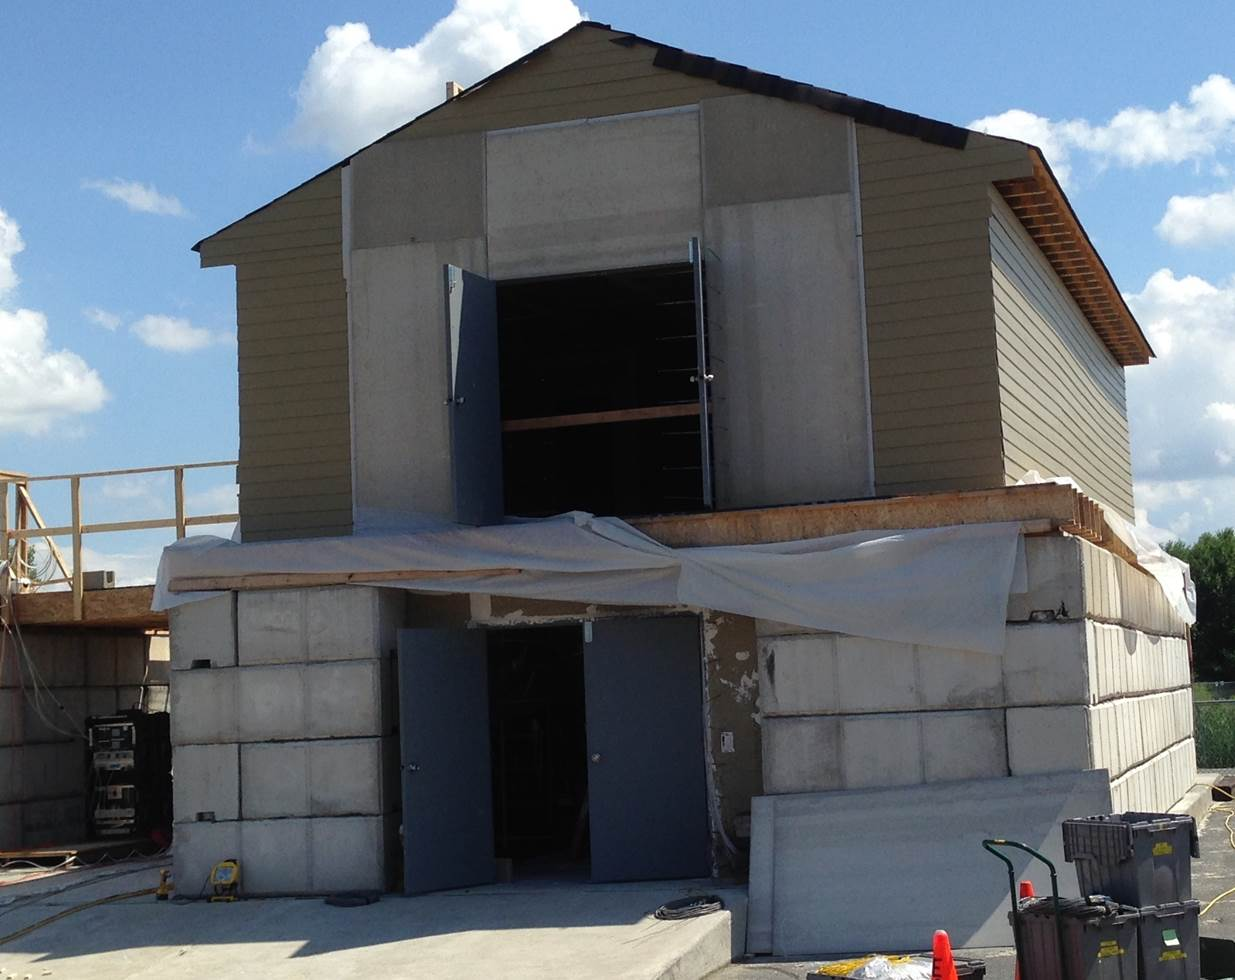
\includegraphics[width=5.25in]{Figures/Pictures/west_structure}
	\caption[North side of the East and West Structures]{North side of the East Structure (top) and West Structure (bottom).}
	\label{fig:struct_pics}
\end{figure}

The interior walls on the first floor of each structure were framed with steel studs set to 400~mm (16~in) centers and track. Two layers of 16~mm (0.63~in) Type X gypsum board lined the steel studs, and a layer of 13~mm (0.5~in) thick Durock cement board covered the gypsum board. The interior ceiling of each structure was covered by two layers of 13~mm (0.5~in) thick Durock cement board.

The first floor ceiling support of each structure was composed of wood truss joist I-beams (TJIs). Each TJI had a depth of 298~mm (11.75~in) and contained laminated veneer lumber flanges with a cross section of 29~mm (1.13~in) by 44~mm (1.75~in) and an 11~mm (0.43~in) thick oriented strand board (OSB) web as shown in Figure~\ref{fig:TJI}. A layer of 18.3~mm (0.72~in) thick tongue and groove OSB was attached to the top of the TJIs.

\begin{figure}[!h]
	\centering
	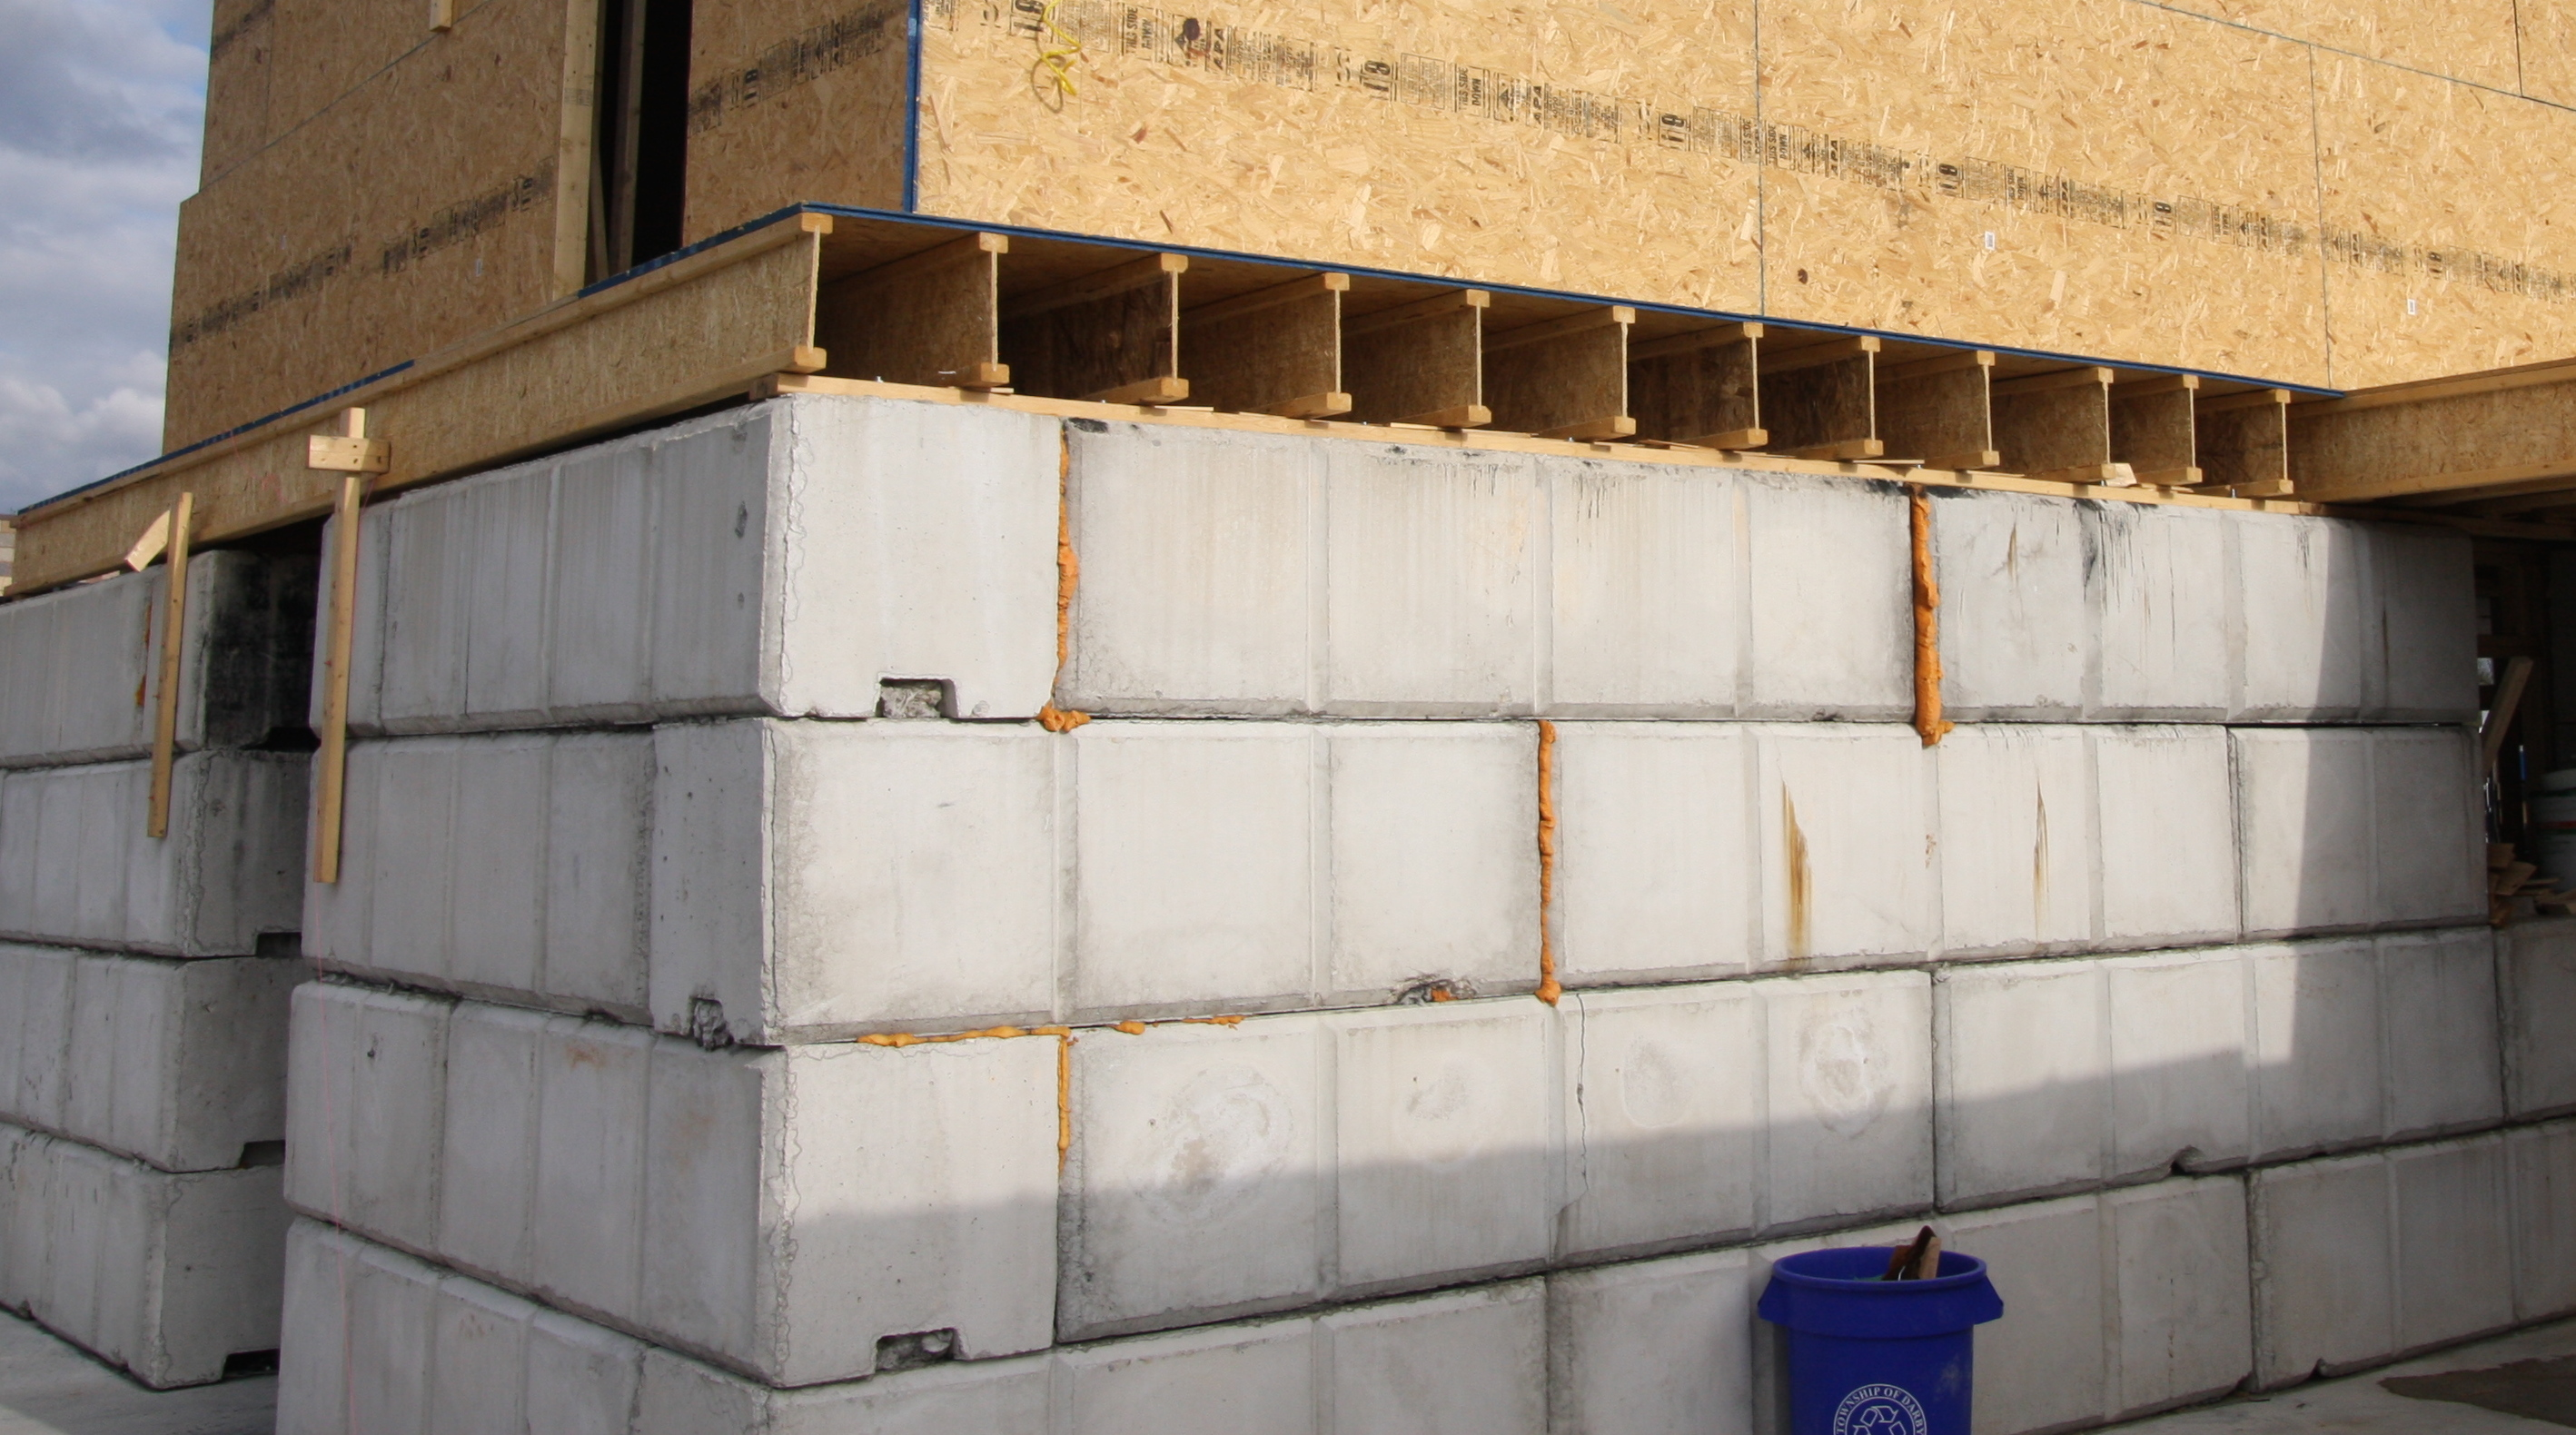
\includegraphics[width=6in]{Figures/Pictures/TJI_support}
	\caption[Ceiling support of the West Structure]{First floor ceiling support of the West Structure composed of wood truss joist I-beams. View is of the southeast corner of the structure.}
	\label{fig:TJI}
\end{figure}

\subsubsection*{\textit{Second Floor of West Structure}}
The second floor of the West Structure was built on the structure's first floor wood ceiling support. The two floors were connected by an interior stairwell. A door made of lauan plywood was located at the top of the stairwell. The walls on the second floor were of wood frame with 51~mm (2~in) by 102~mm (4~in) studs set to 400~mm (16~in) centers. Two layers of 16~mm (0.63~in) Type X gypsum board lined the interior side of the wood studs, and a layer of 13~mm (0.5~in) thick Durock cement board covered the gypsum board. The interior ceiling of the second story was covered by two layers of 13~mm (0.5~in) thick Durock cement board. The exterior sides of the outer walls on the second floor were protected by 11~mm (0.44~in) thick OSB and 8~mm (0.31~in) fiber cement lap siding.

\subsubsection*{\textit{Leakage}}
An air leakage measurement system~\cite{INFILTEC:leakage} from Infiltec, Inc. (model E3-A-DM4), was used to measure the amount of leakage associated with each structure. The amount of leakage in the East Structure was measured as 0.024~m$^2$. For the West Structure, the leakage was measured as 0.027~m$^2$ when the stairway door was fully closed, 0.054~m$^2$ when the stairway door was fully opened, and 0.048~m$^2$ when the stairway door was in the ``closed'' position (having a 152~mm (6~in) gap between the door and the frame) used during Tests~24 and 25.

\subsection{Layout}

Dimensioned floor plans of the East and West Structures are presented in Figures~\ref{fig:east_dimensioned_plan}~and~\ref{fig:west_dimensioned_plan}, respectively.

\begin{figure}[!h]
	\centering
	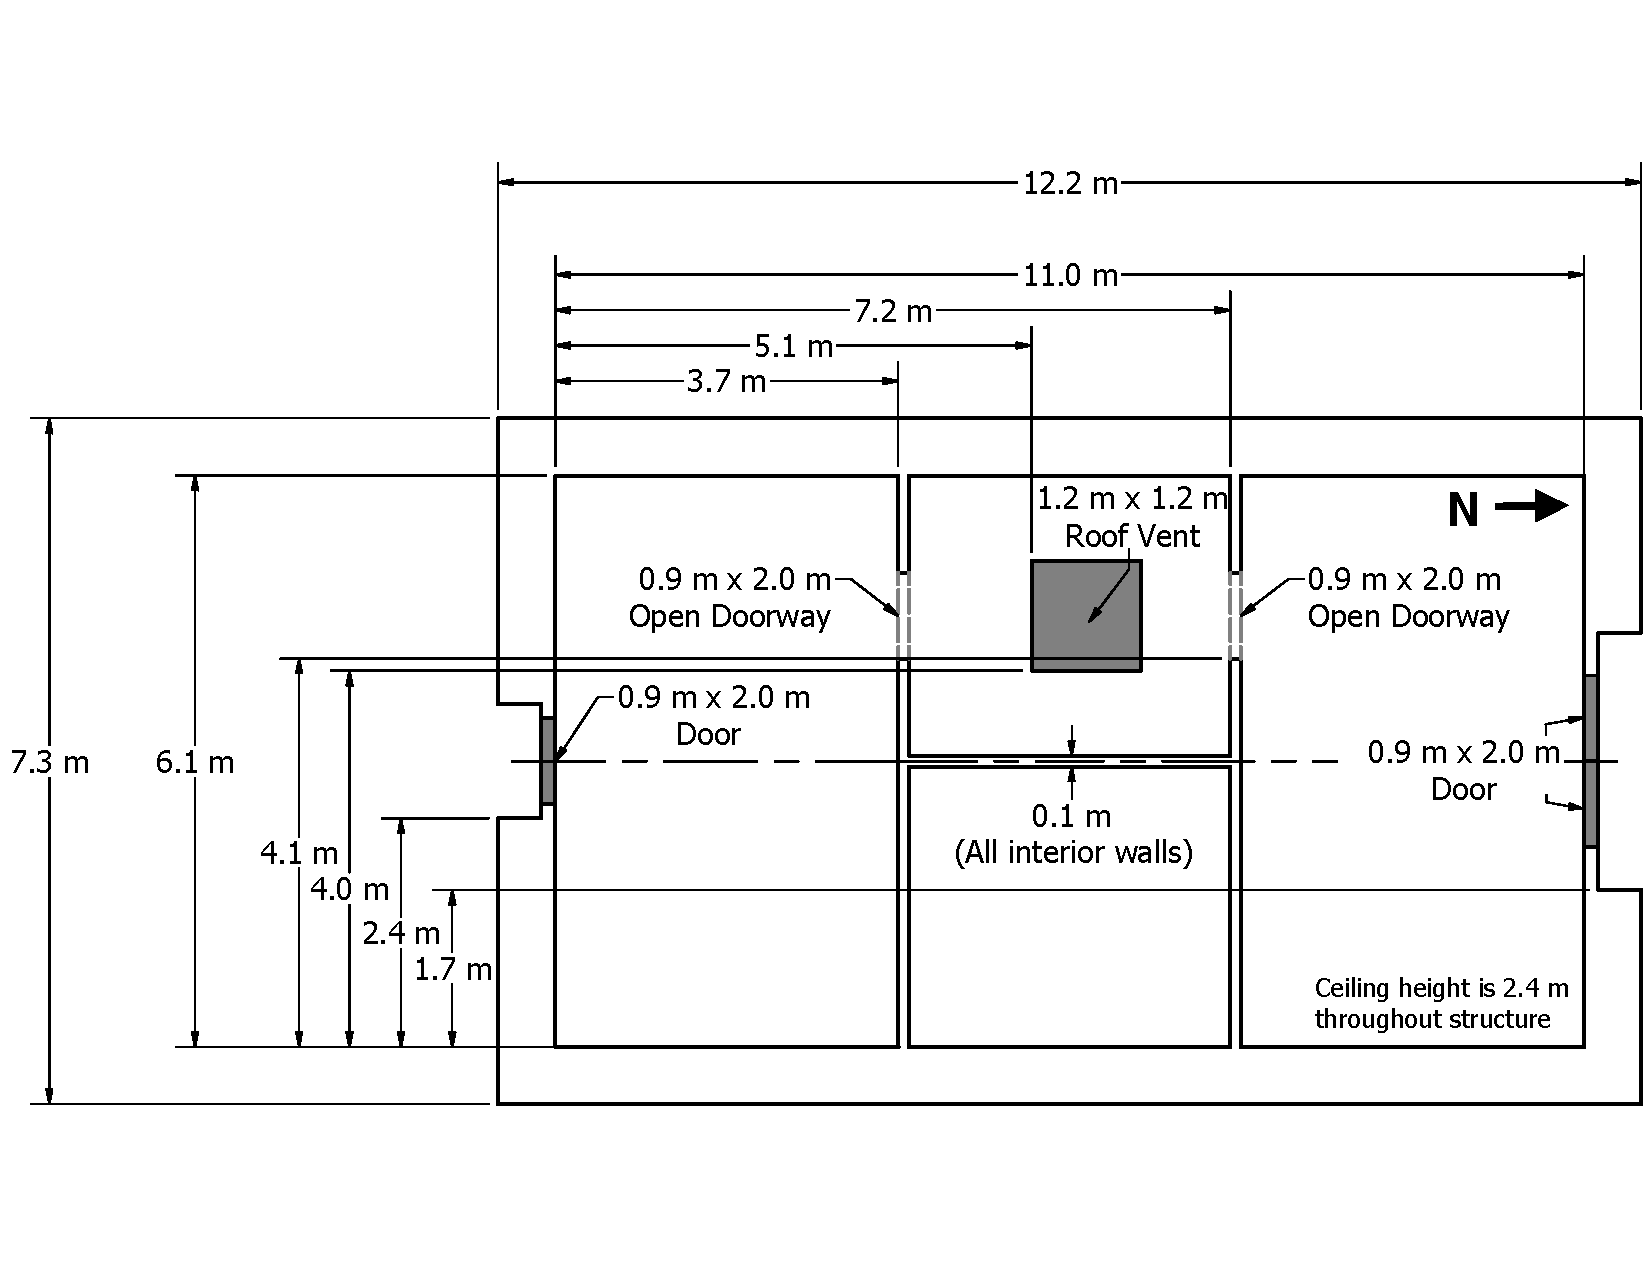
\includegraphics[width=\columnwidth]{Figures/Floor_Plans/East_Structure_Dimensioned_Full}
	\caption[Dimensioned floor plan of the East Structure]{Dimensioned floor plan of the East Structure. Structure dimensions are symmetric across horizontal centerline.}
	\label{fig:east_dimensioned_plan}
\end{figure}

\begin{figure}[!h]
	\centering
	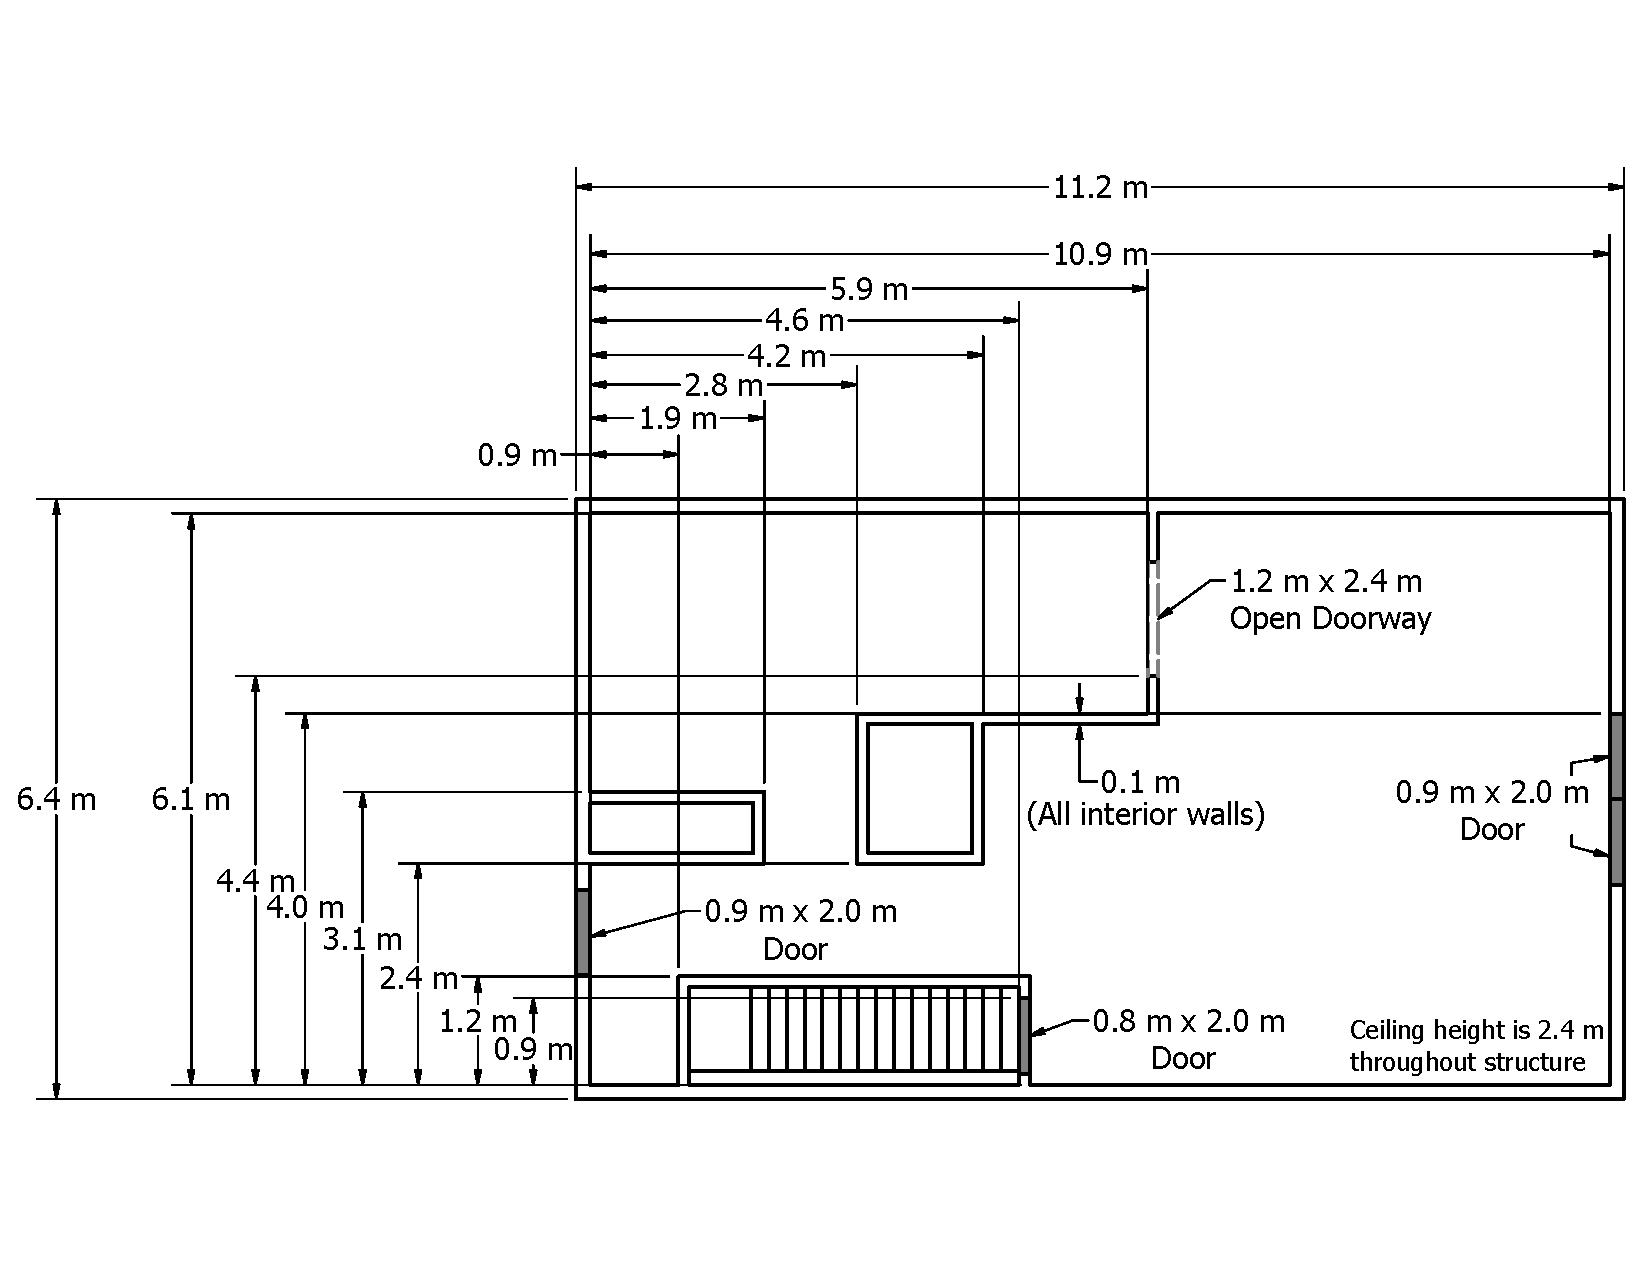
\includegraphics[width=\columnwidth]{Figures/Floor_Plans/West_Structure_2nd_Floor_Dimensioned_Full}
	\\~\\
	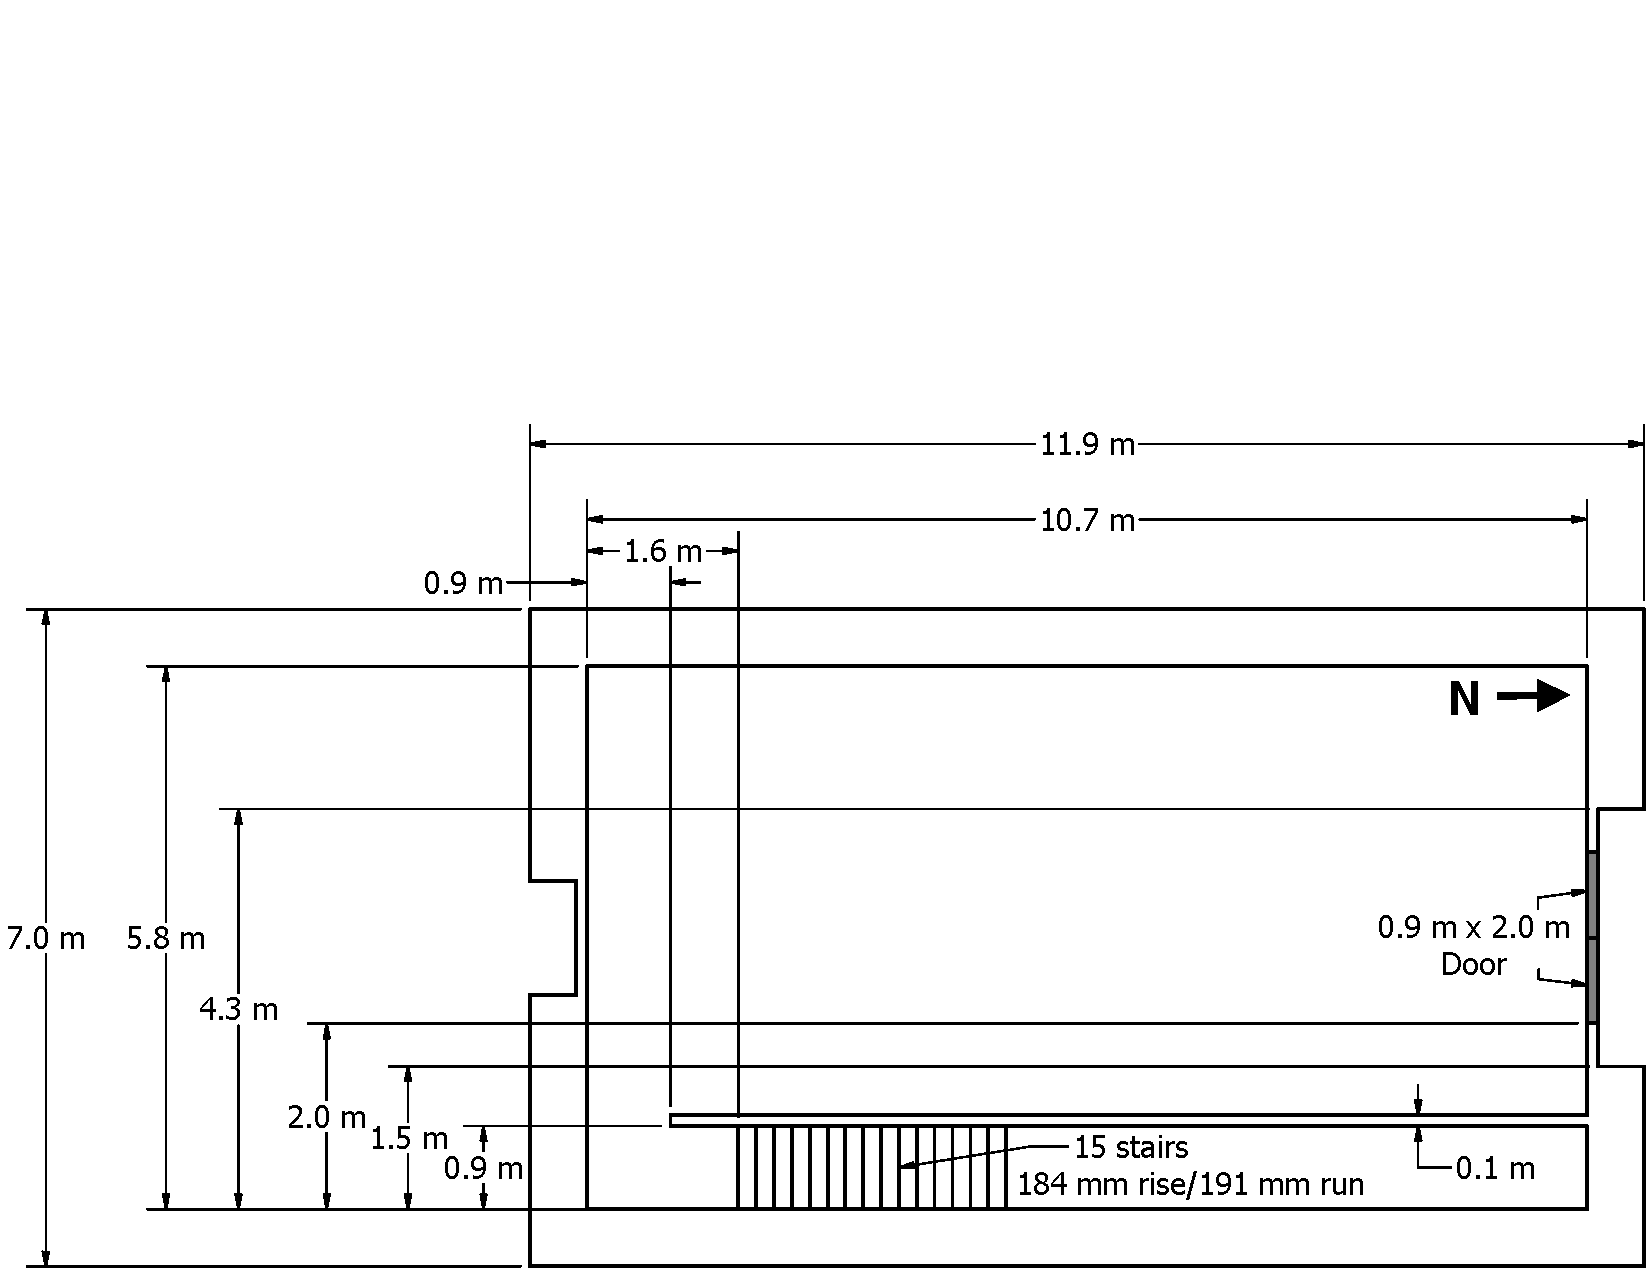
\includegraphics[width=\columnwidth]{Figures/Floor_Plans/West_Structure_1st_Floor_Dimensioned_Full}
	\caption[Dimensioned floor plans of the West Structure]{Dimensioned floor plan of the second floor (top) and first floor (bottom) of the West Structure.}
	\label{fig:west_dimensioned_plan}
\end{figure}

The exterior doors of both structures, the stairwell door in the West Structure, and the square roof vent with a depth of 320~mm (12.75~in) in the East Structure were opened and closed at certain instances during the experiments to change the ventilation patterns within the structures.

\clearpage
\section{Instrumentation}
\label{sec:intrumentation}
The structures were instrumented for temperature, gas velocity, heat flux, and gas concentration measurements. Gas temperatures in the burn rooms were measured with bare-bead, Chromel-Alumel (type K) thermocouples. Additional single thermocouples were installed in conjunction with bi-directional probes for gas velocity measurements. The single thermocouples were bare-bead, Chromel-Alumel (type K) thermocouples with a 1.0~mm (0.04~in) nominal diameter. The thermocouple wire was protected with a 3.2~mm (0.13~in) diameter inconel sheath. Water-cooled Schmidt-Boelter gauges were used to measure the total heat flux at different locations throughout the structures. Calibrated pumps pulled gas samples through a sample conditioning system to eliminate moisture in the sample. Then, the dry gas samples were piped to a series of gas analyzers and the gas concentrations of oxygen and carbon dioxide were measured. A legend is presented in Figure~\ref{fig:Instrumentation_Legend} to clarify the instrumentation schematic diagrams presented in the follow sections.

\begin{figure}[!h]
	\centering
	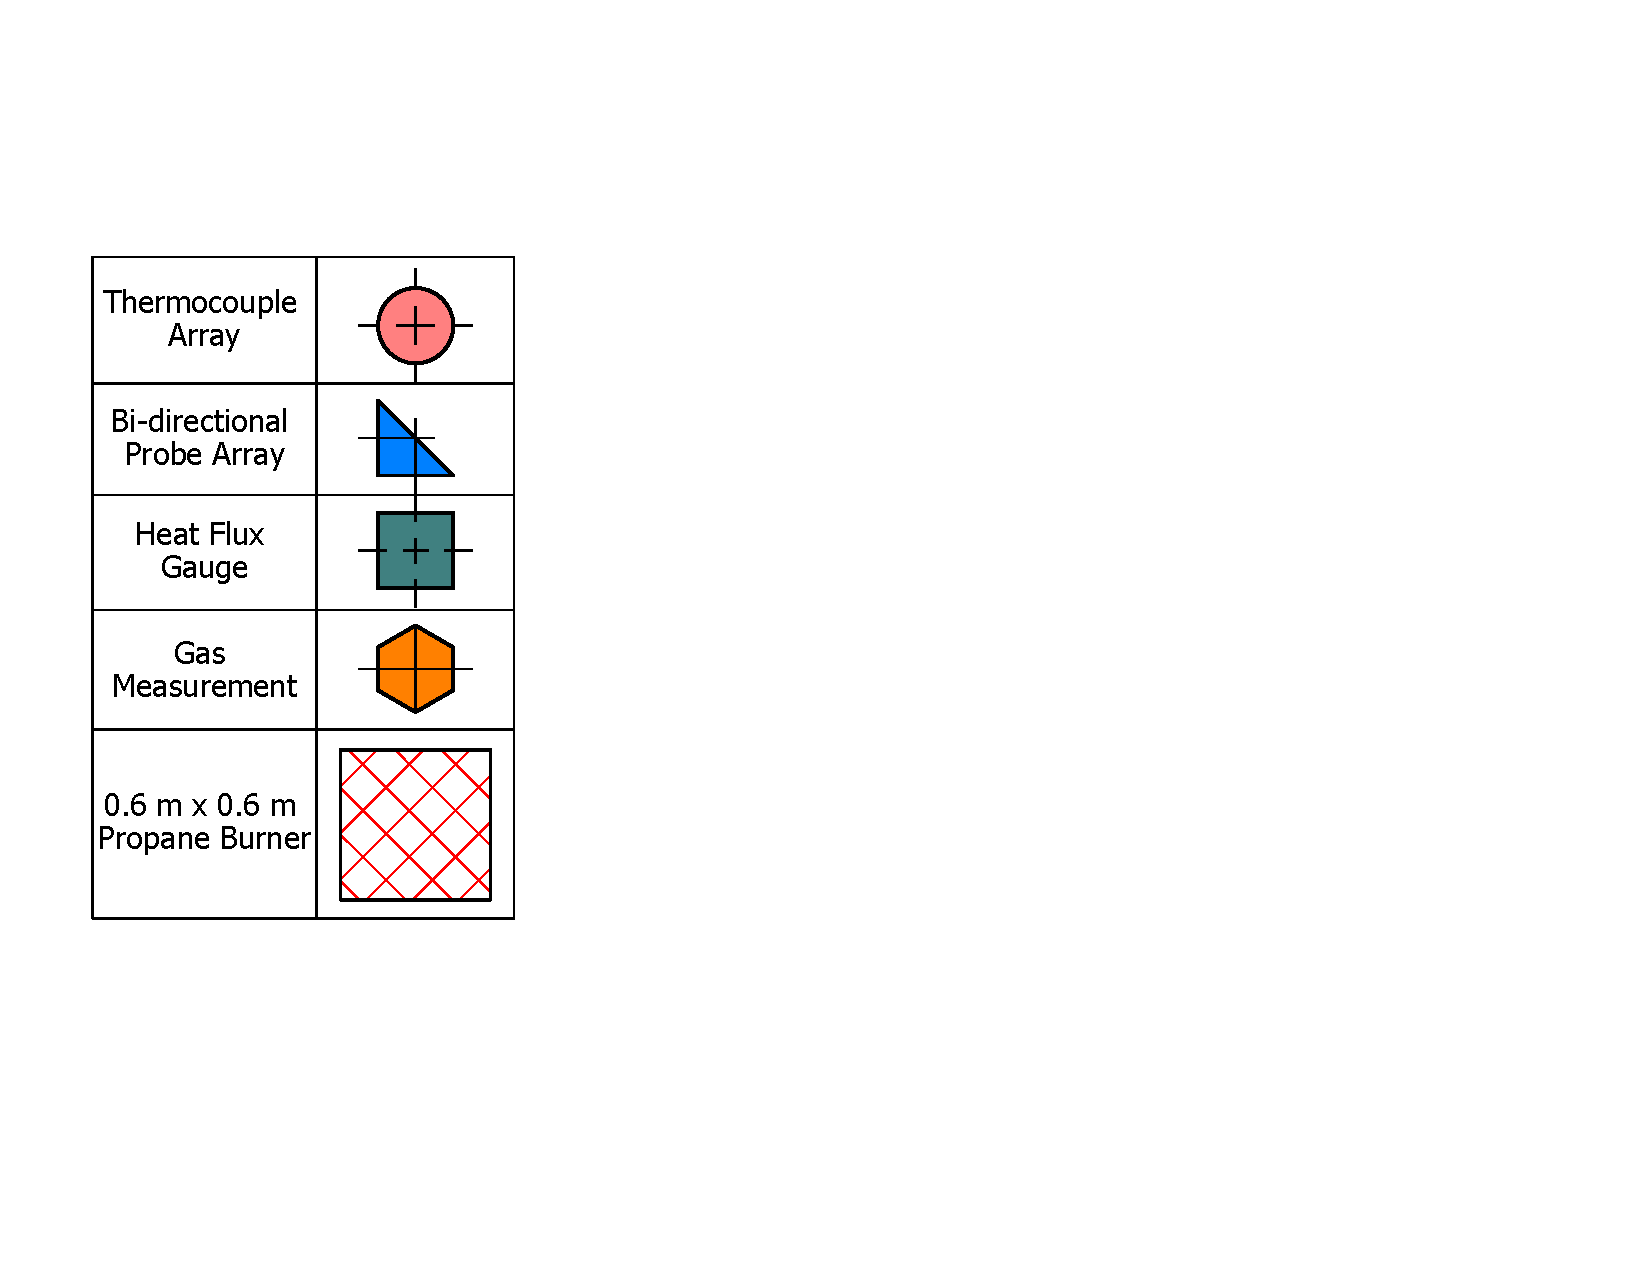
\includegraphics[width=0.25\columnwidth]{Figures/Floor_Plans/Instrumentation_Legend}
	% \begin{quote}
	\caption[Instrumentation legend]{Legend used for schematic diagrams of instrumentation locations.}
	% \end{quote}
	\label{fig:Instrumentation_Legend}
\end{figure}

Three diffusion flame burners, pictured in Figure~\ref{fig:burners}, were used as the fuel source for each experiment. Each burner had a square opening of side length 0.6~m (2~ft) located 0.14~m (5.5~in) above the floor and were positioned 0.6~m (2~ft) from the interior side of the south and west walls on the ground floor of each structure. Propane was flowed from a supply truck to the gas burners for all experiments. The flow of propane to each burner was controlled by a high-precision turn valve, and the total displaced gas volume was measured using a rotary gas meter.

\begin{figure}[!h]
	\centering
	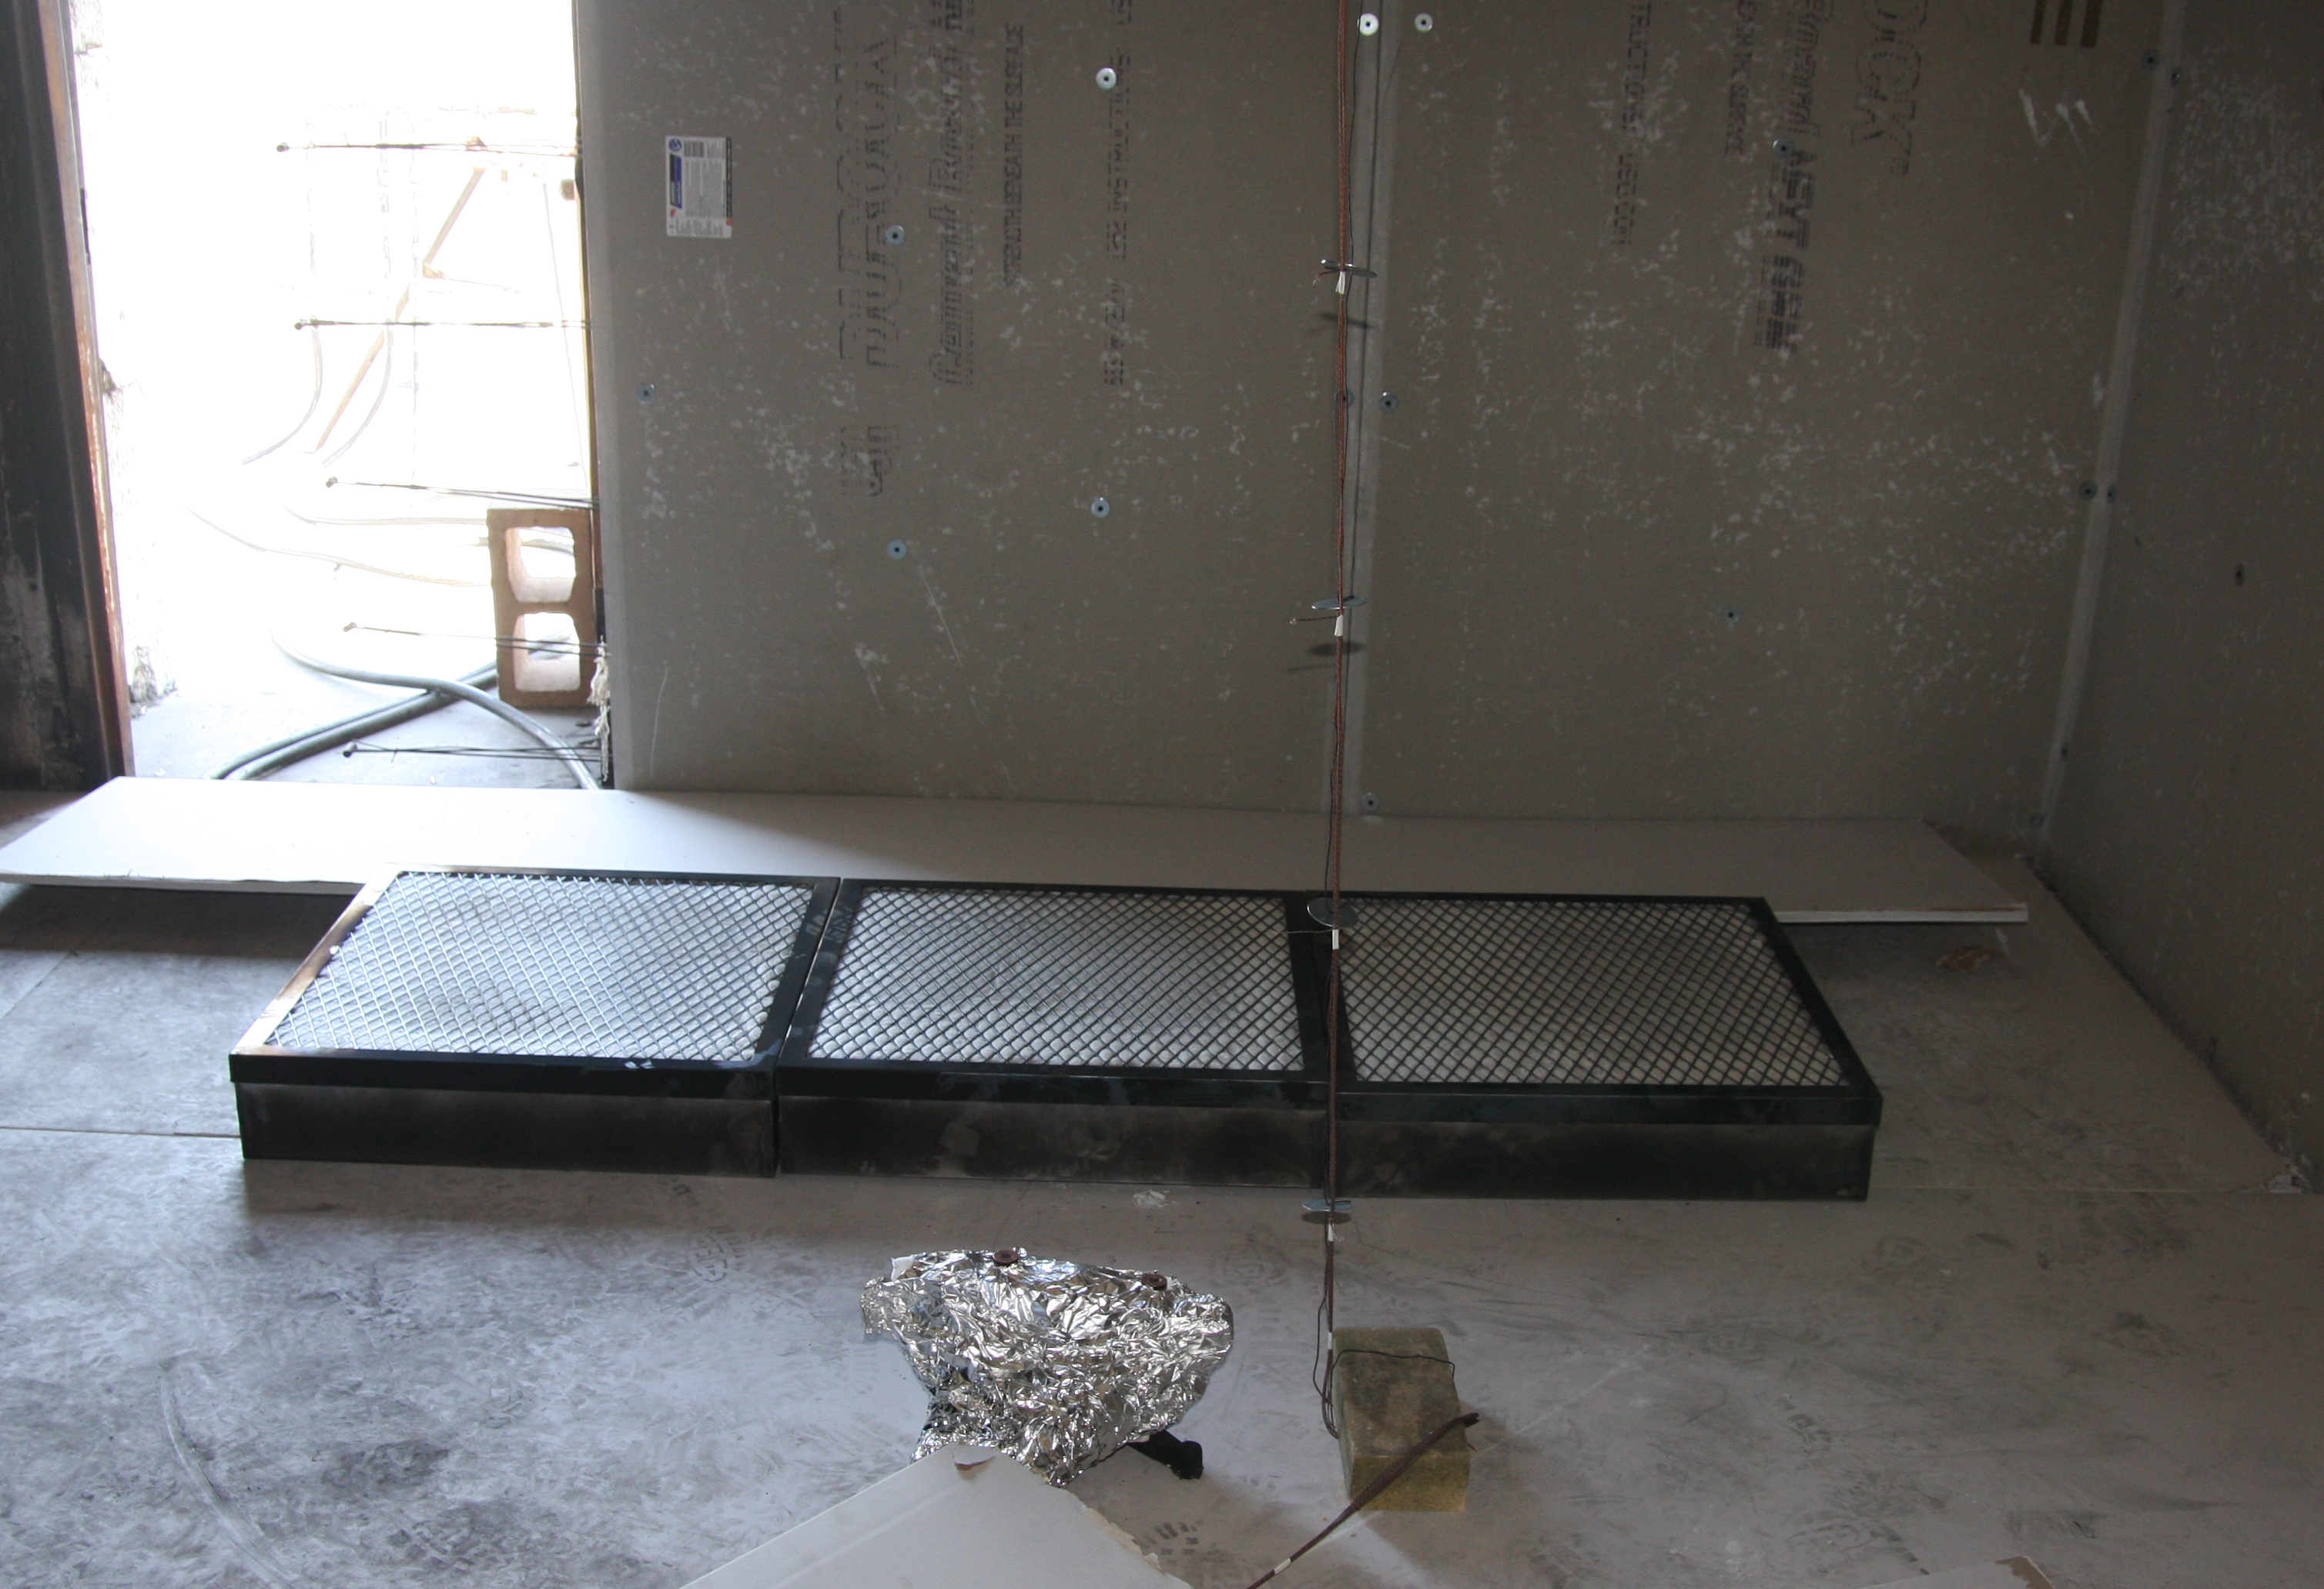
\includegraphics[width=0.9\columnwidth]{Figures/Pictures/burners}
	\caption[Three propane burners used as the fuel source.]{Three propane burners used as the fire source for the experiments located 0.6~m (2~ft) off the interior side of the south and west walls in the East Structure.}
	\label{fig:burners}
\end{figure}
\FloatBarrier

\subsection{East Structure}
The East Structure was instrumented with five bare-bead thermocouple arrays, four bi-directional probe plus solid thermocouple arrays, four total heat flux gauges, and two gas sample inlet pipes at the locations shown in Figure~\ref{fig:east_instrumentation}.

\begin{figure}[!h]
	\centering
	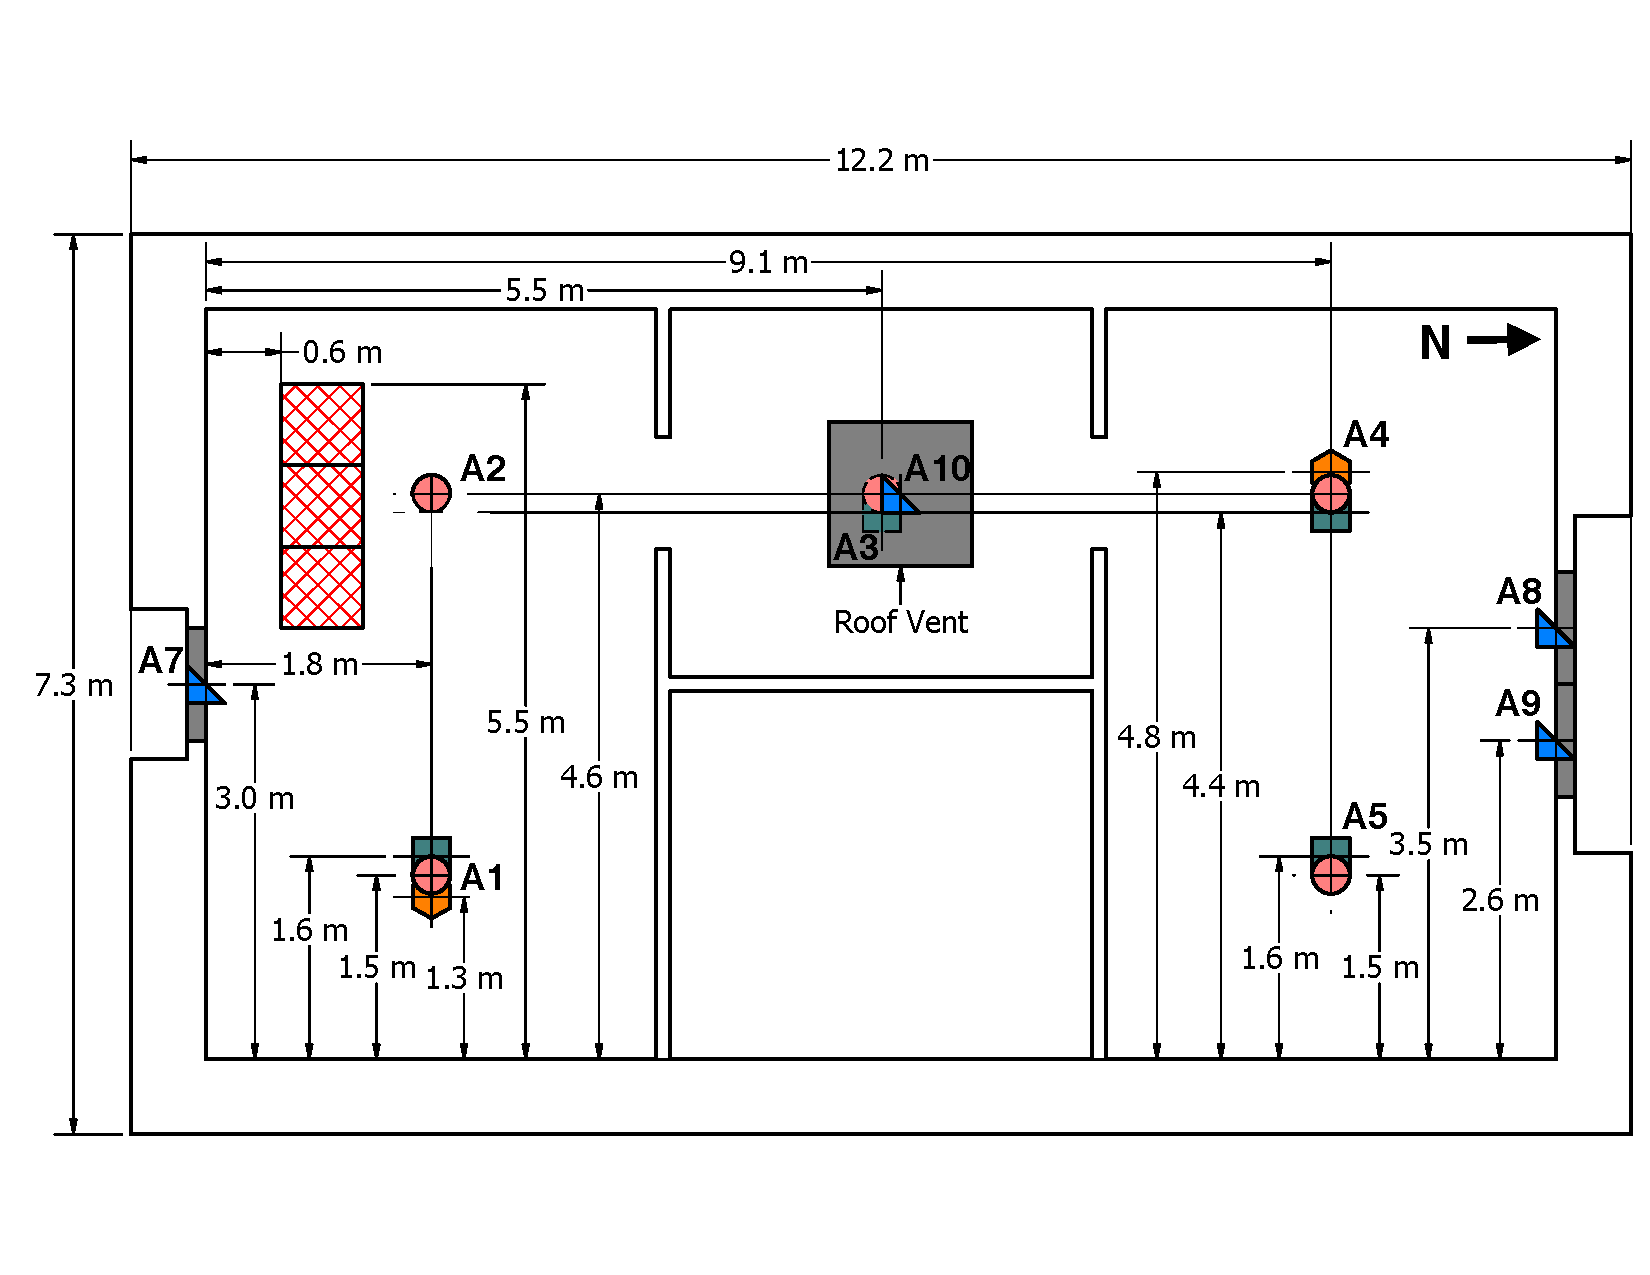
\includegraphics[width=\columnwidth]{Figures/Floor_Plans/East_Structure_Dimensioned_Instrumentation_New}
	\caption[Locations and labels of instrumentation in the East Structure]{Locations and labels of instrumentation in the East Structure.}
	\label{fig:east_instrumentation}
\end{figure}

Each bare-bead thermocouple array (A1, A2, A3, A4, and A5) was composed of eight vertically-aligned thermocouples spaced between the floor and ceiling. Three bi-directional probe and solid thermocouple arrays (A7, A8, and A9) were centered in the exterior doorways of the structure and contained eight probes as shown in Figure~\ref{fig:BDP_arrays}. The fourth bi-directional probe and solid thermocouple array (A10), also presented in Figure~\ref{fig:BDP_arrays}, was located at the opening of the roof vent, 320~mm (12.75~in) above the compartment ceiling. The array contained three probes centered between the east and west sides of the vent. The position of each probe and thermocouple pair relative to the south wall of the vent is listed in Table~\ref{table:east_channel_list} of Appendix~\ref{chap:channel_lists}. The total heat flux gauges (A1, A3, A4, and A5) were located near the floor and aimed to view the ceiling. Lastly, gas samples were pulled from the environment through 9.5~mm (0.38~in) diameter stainless steel tubing (A1 and A4). The height of each individual sensor in the sensor arrays is listed in Table~\ref{table:east_channel_list} of Appendix~\ref{chap:channel_lists}.

\begin{figure}[!h]
	\centering
	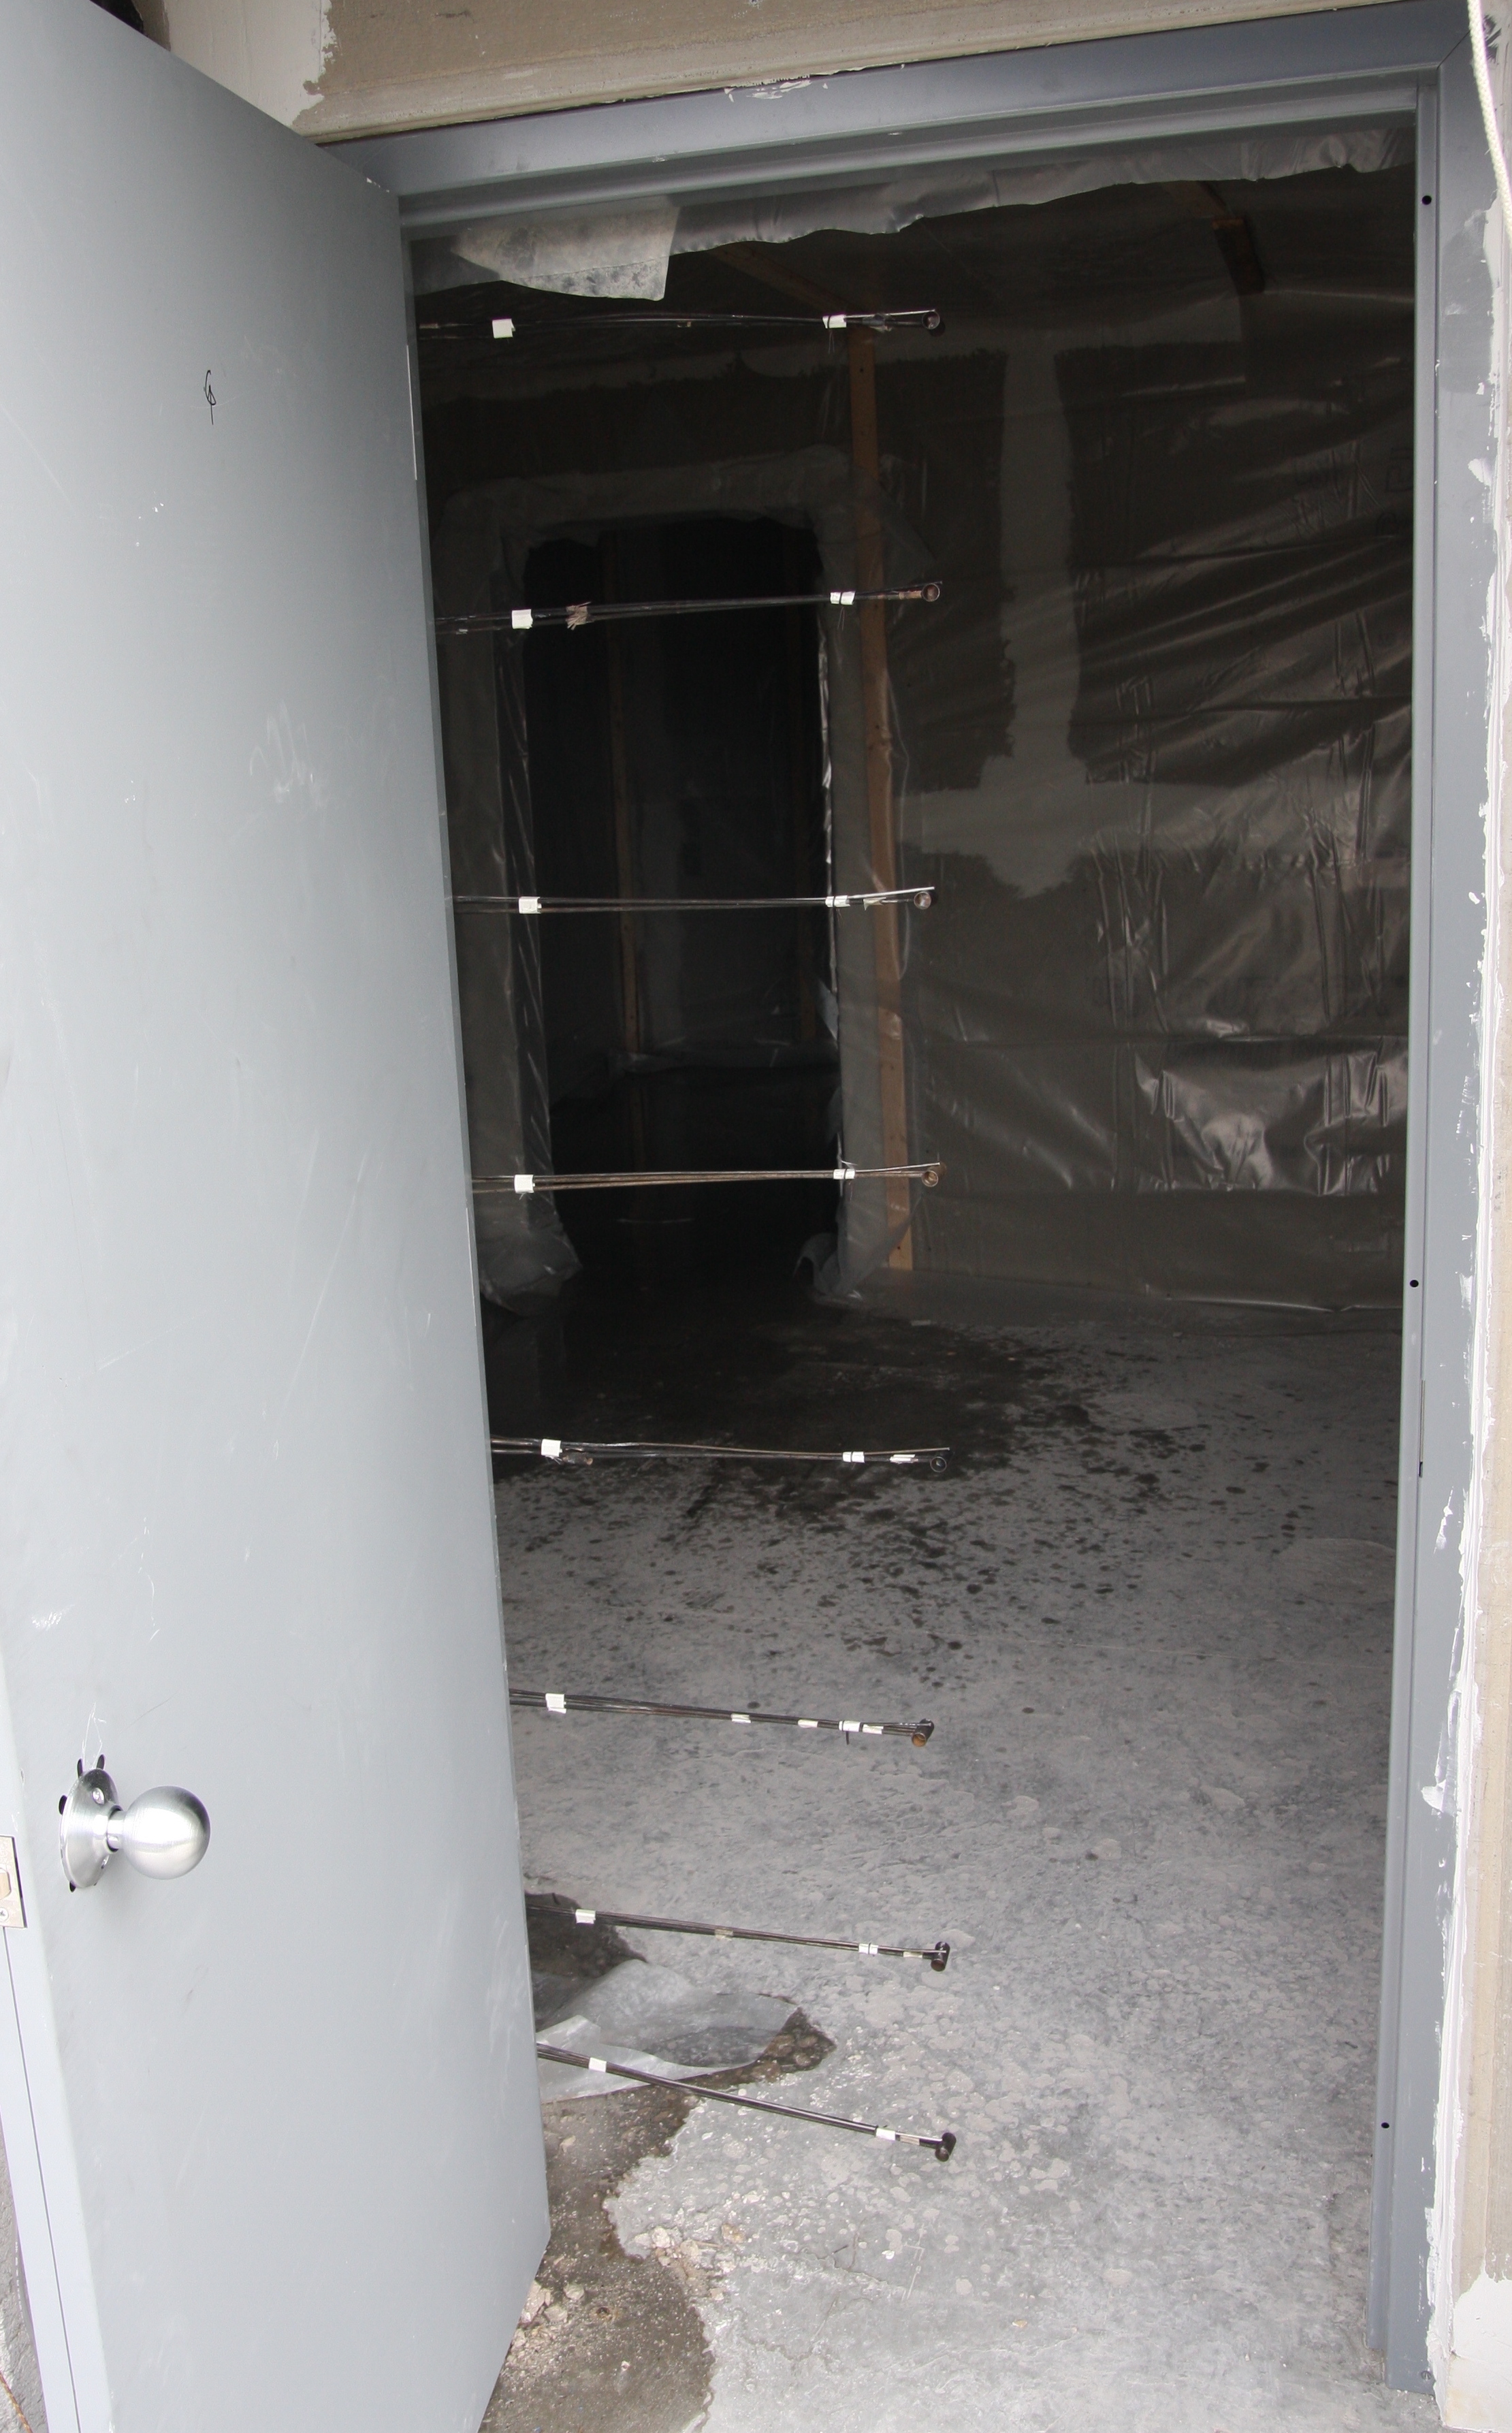
\includegraphics[width=0.35\columnwidth]{Figures/Pictures/doorway_BDPs}
	\\~\\
	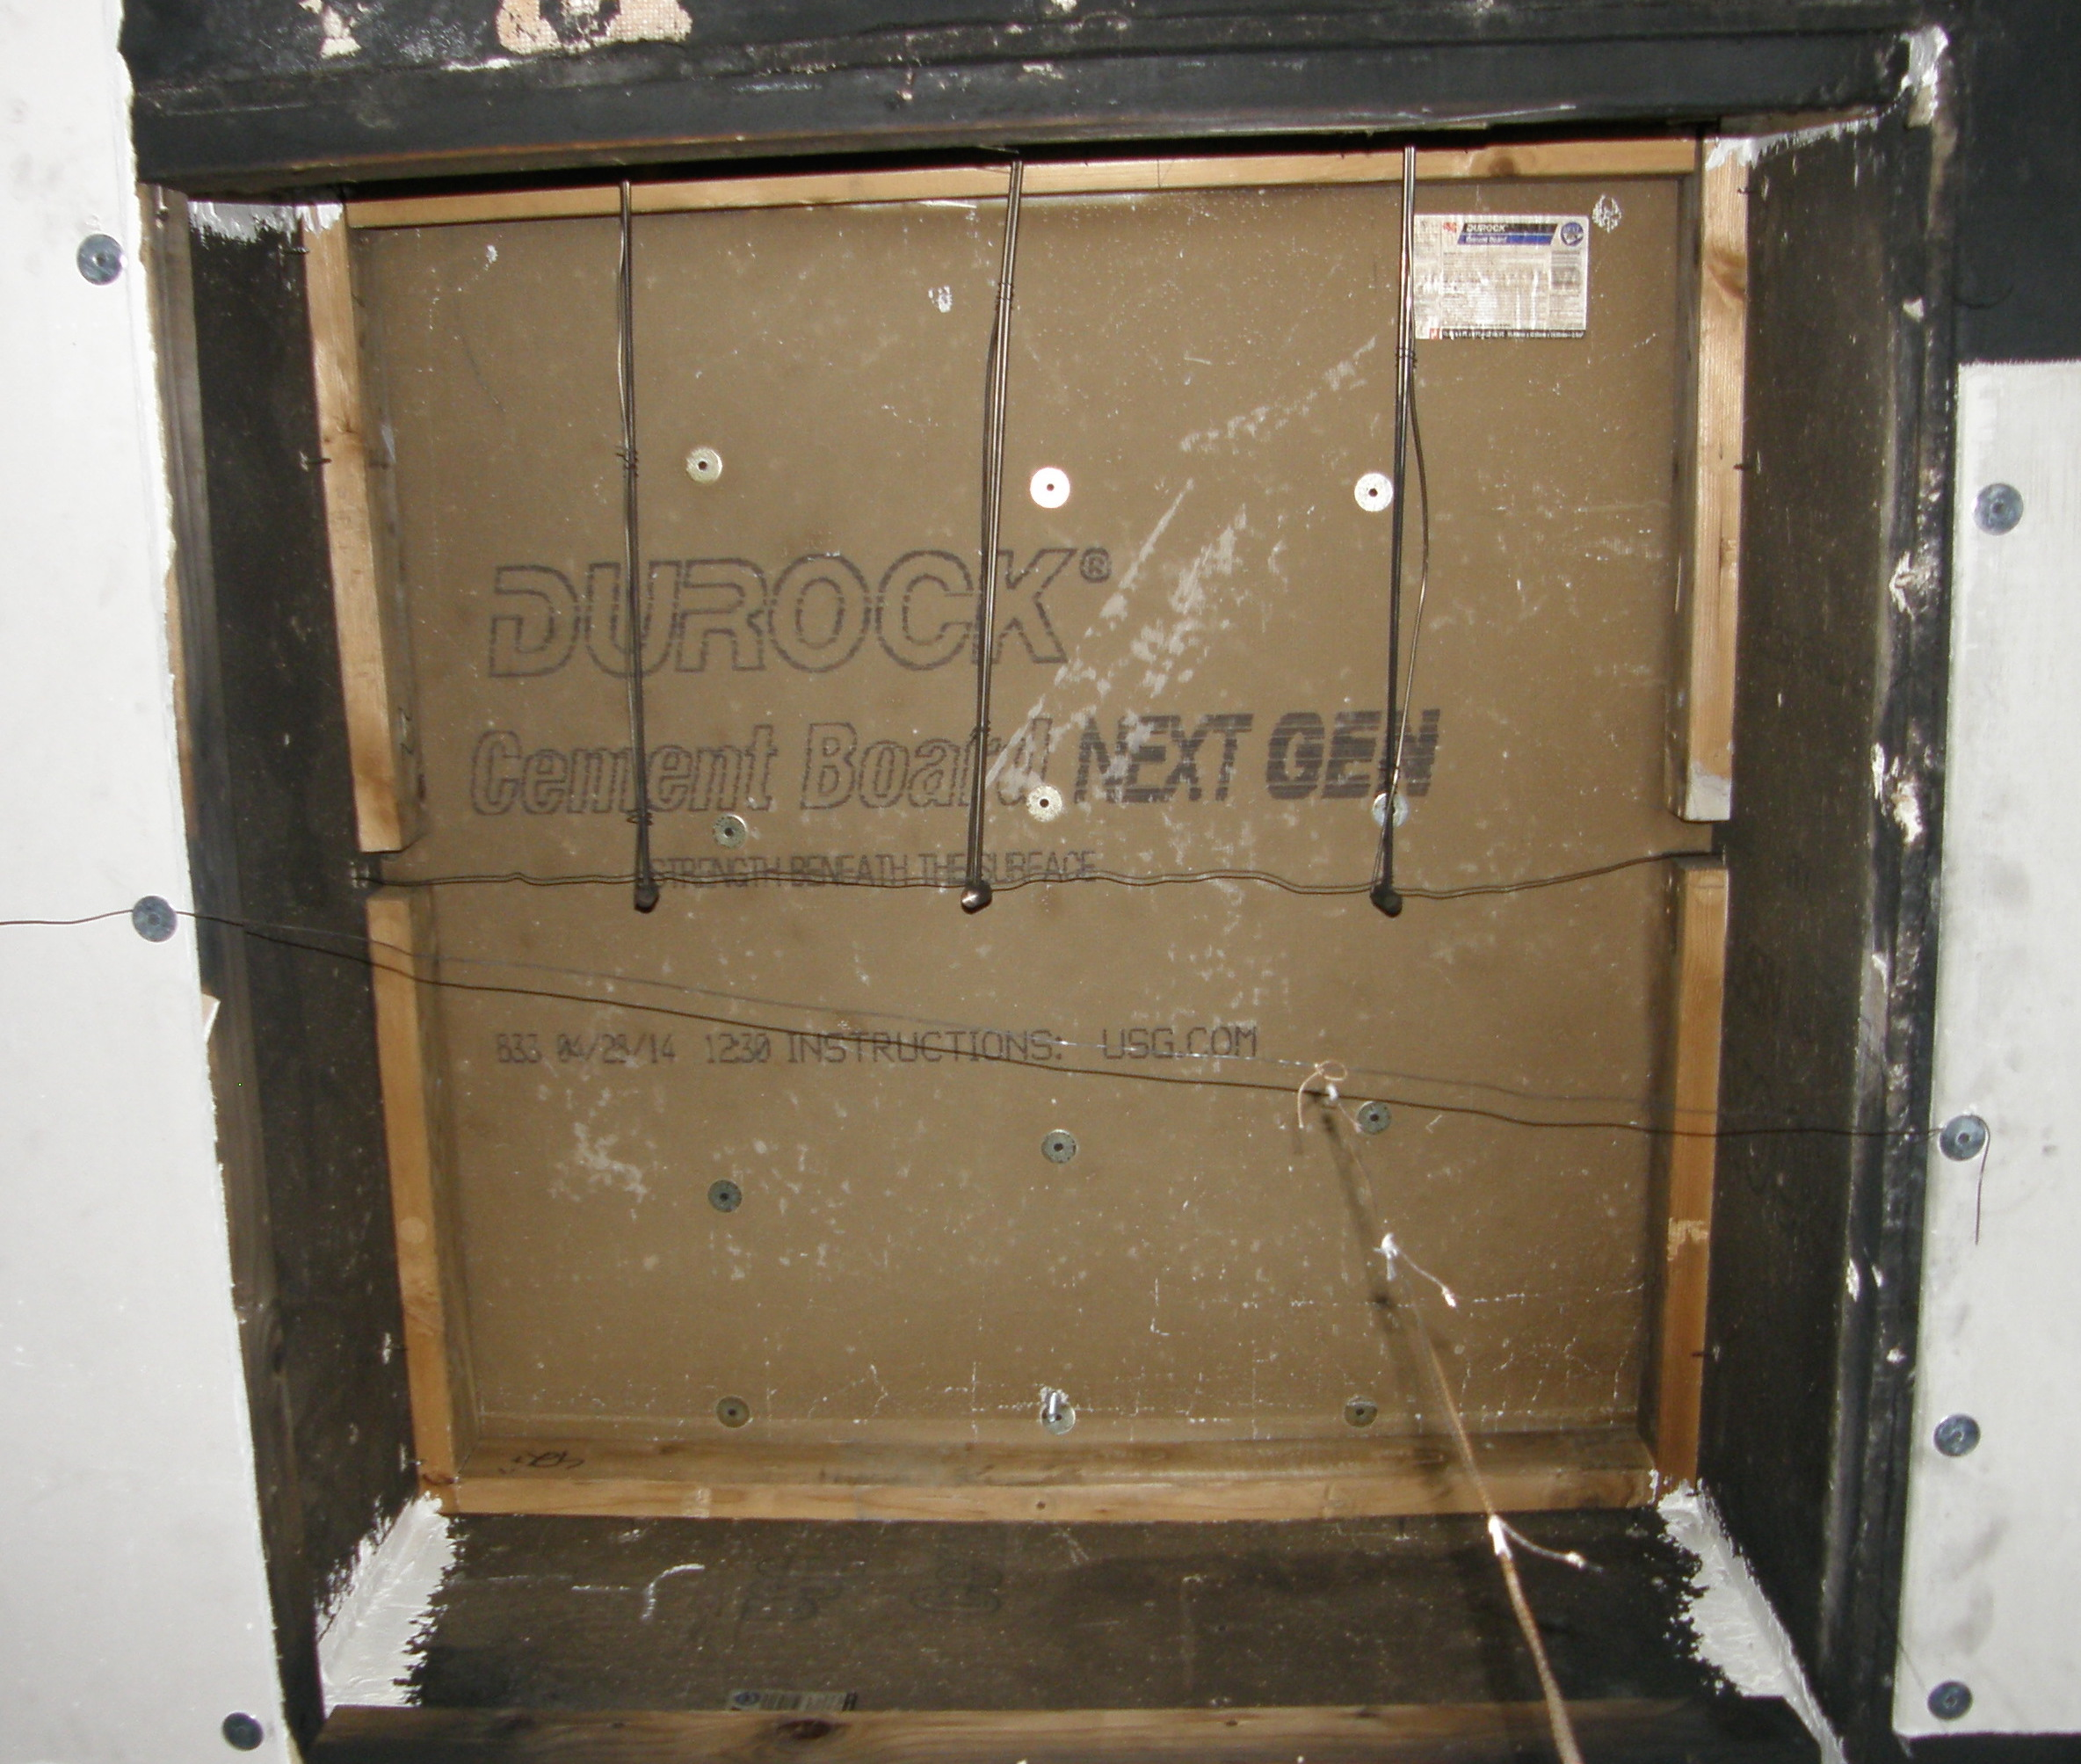
\includegraphics[width=0.55\columnwidth]{Figures/Pictures/roof_vent_BDPs}
	\caption[Bi-directional probe plus solid thermocouple arrays in East Structure]{Bi-directional probe plus solid thermocouple array at the south exterior doorway (top) and roof vent (bottom) of the East Structure.}
	\label{fig:BDP_arrays}
\end{figure}
\FloatBarrier
\subsection{West Structure}
The first floor of the West Structure was instrumented with three bare-bead thermocouple arrays (A1, A2, and A3), two bi-directional probe plus solid thermocouple arrays (A5 and A6), and one gas sample inlet pipe (A1). The second floor was equipped with three bare-bead thermocouple arrays (A7, A8, and A9), four bi-directional probe plus solid thermocouple arrays (A10, A11, A13, and A14), two total heat flux sensor pairs (A16 and A17), and one gas sample inlet pipe (A10). The location of the instrumentation in the West Structure is shown in Figure~\ref{fig:west_instrumentation}.

\begin{figure}[!ht]
	\centering
	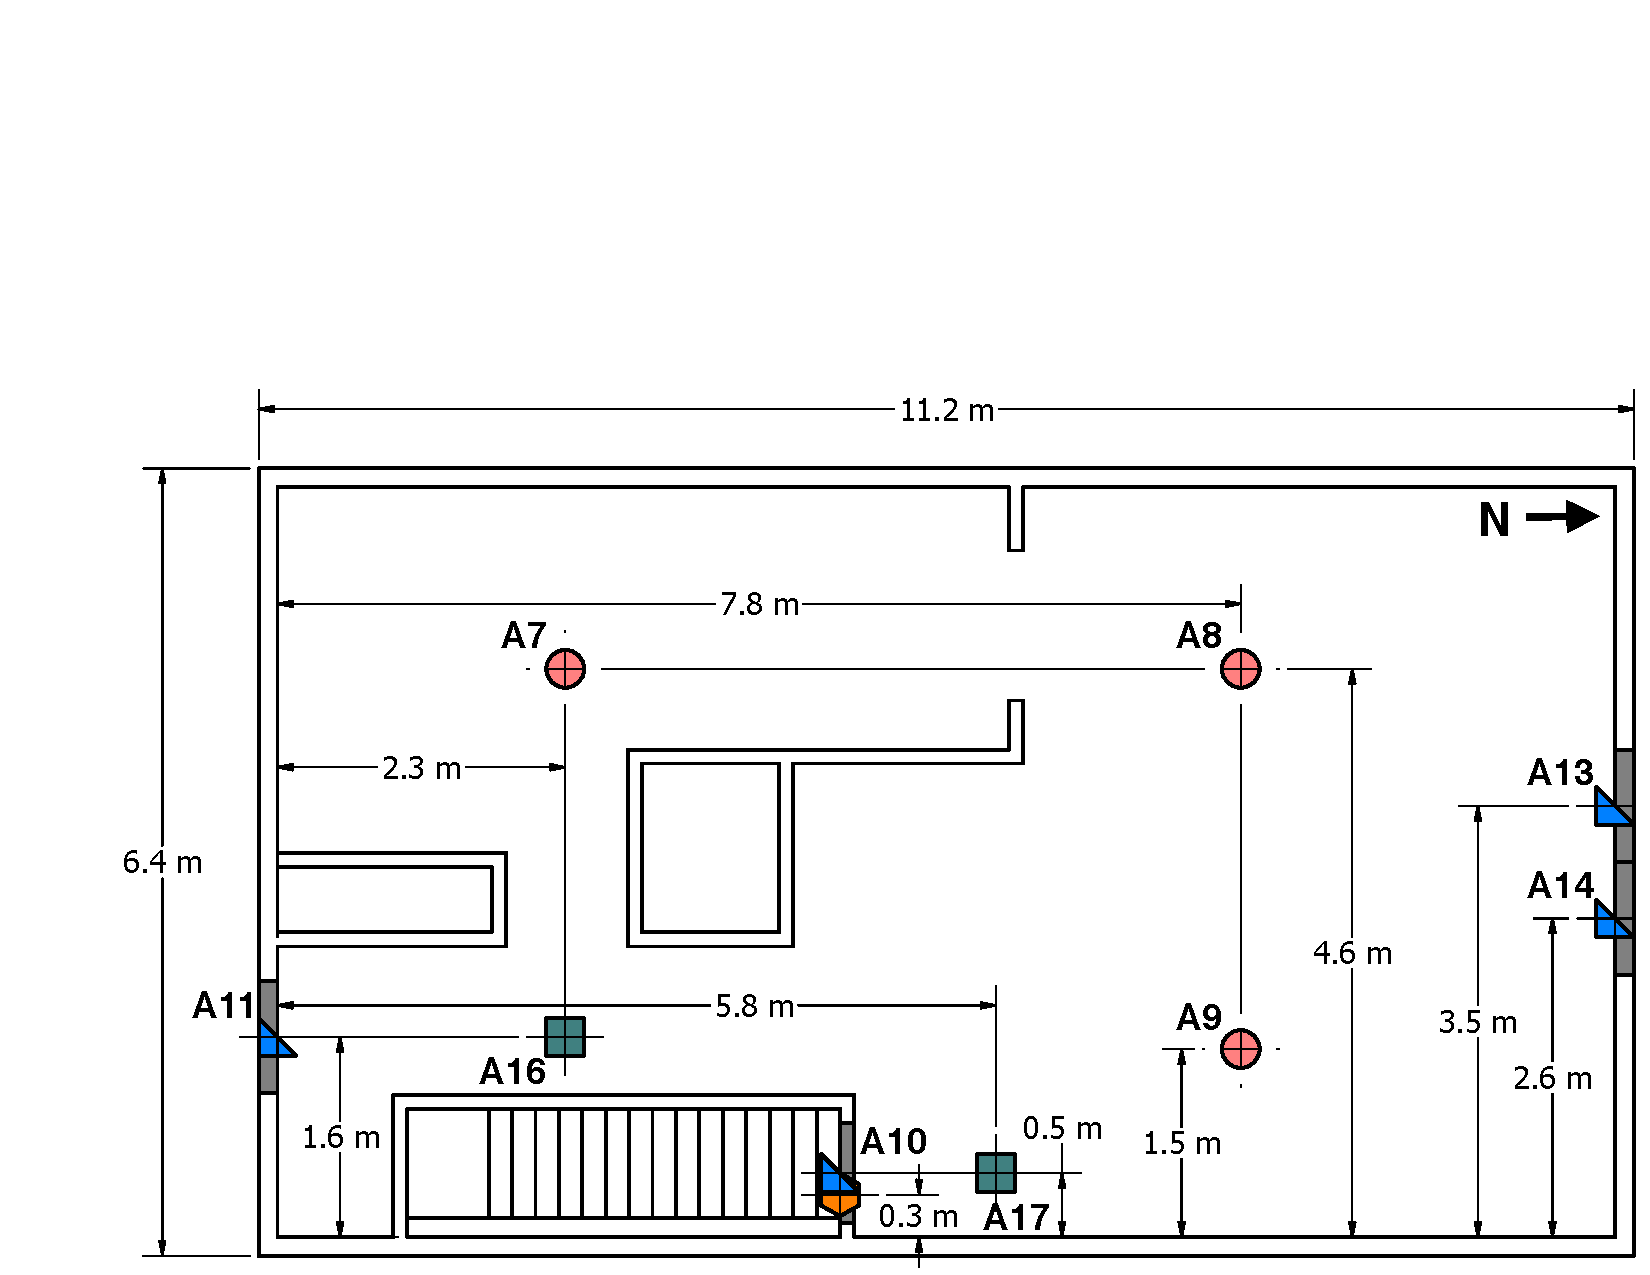
\includegraphics[width=0.94\columnwidth]{Figures/Floor_Plans/West_Structure_2nd_Floor_Dimensioned_Instrumentation}
	\\~\\
	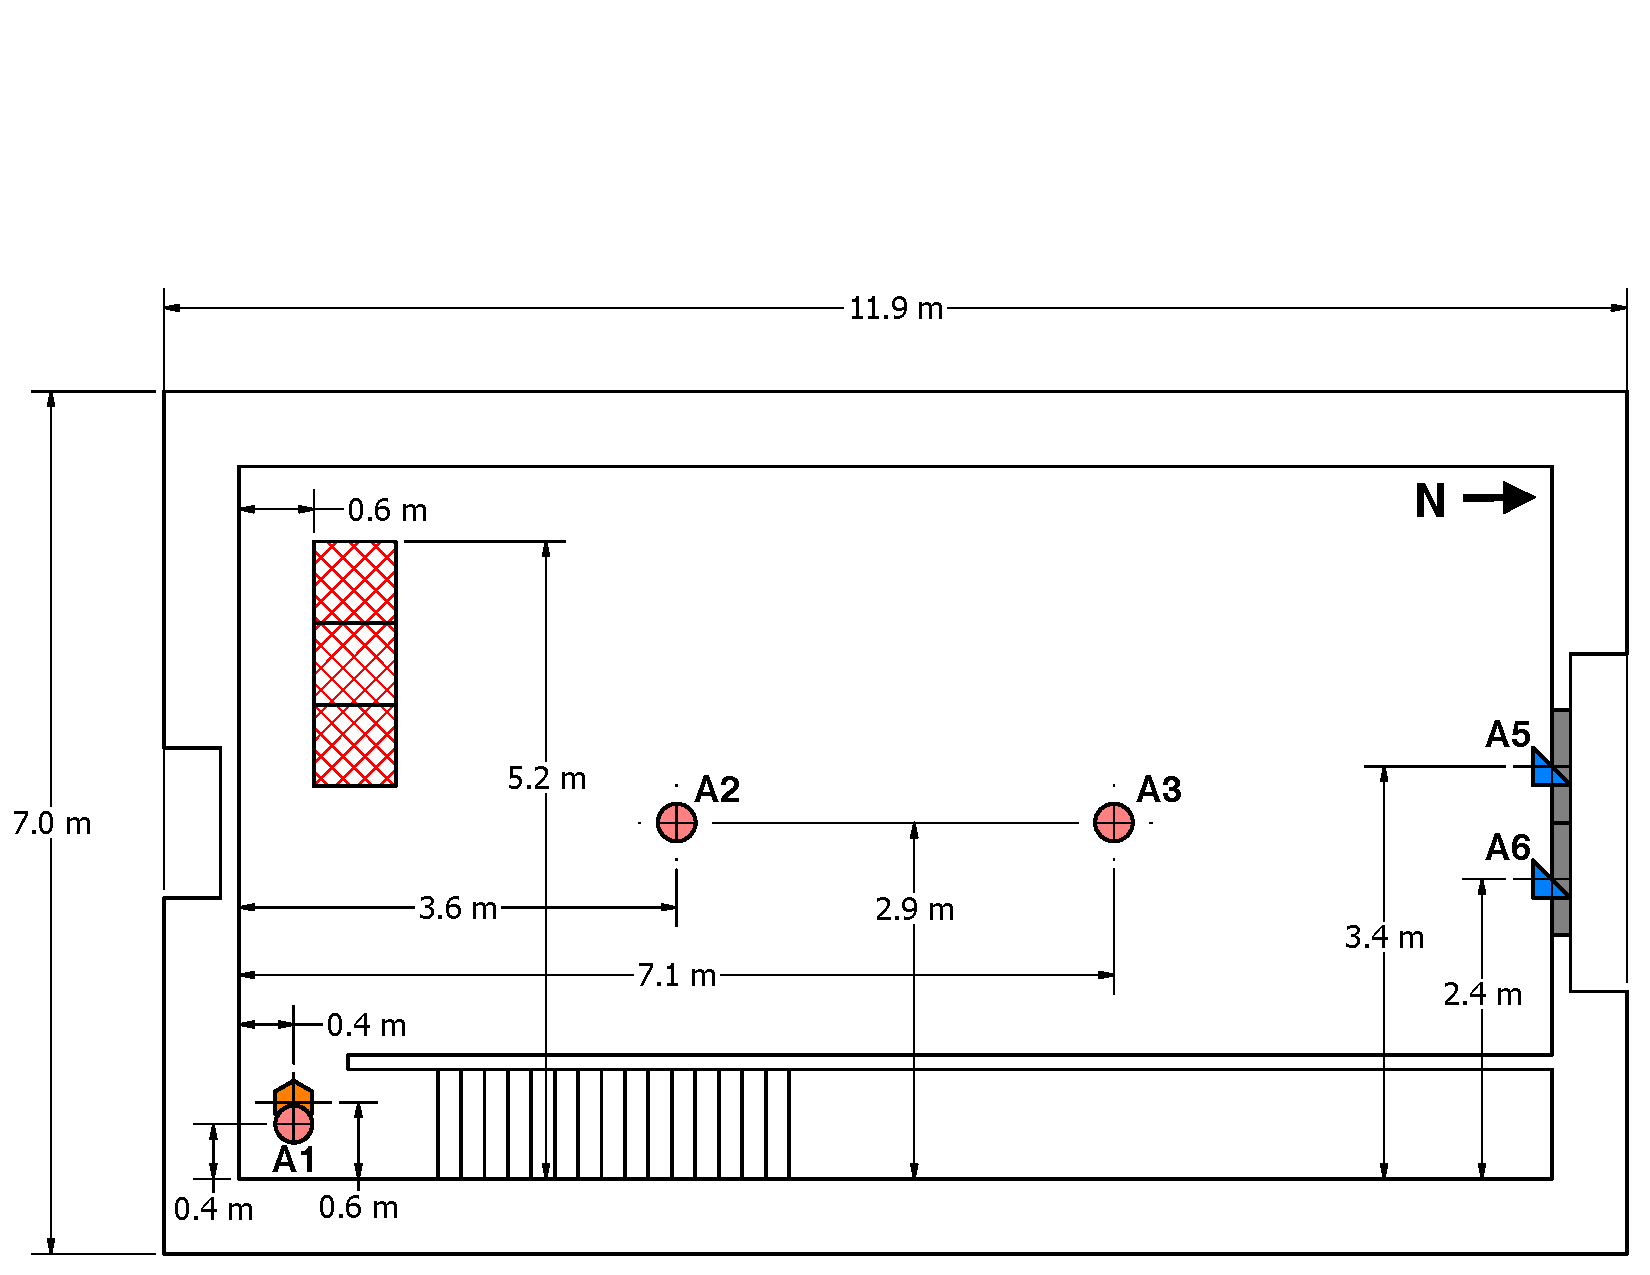
\includegraphics[width=\columnwidth]{Figures/Floor_Plans/West_Structure_1st_Floor_Dimensioned_Instrumentation}
	\caption[Locations and labels of instrumentation in the West Structure.]{Locations and labels of instrumentation in the second floor (top) and first floor (bottom) of the West Structure.}
	\label{fig:west_instrumentation}
\end{figure}

% \begin{figure}
% 	\centering
% 	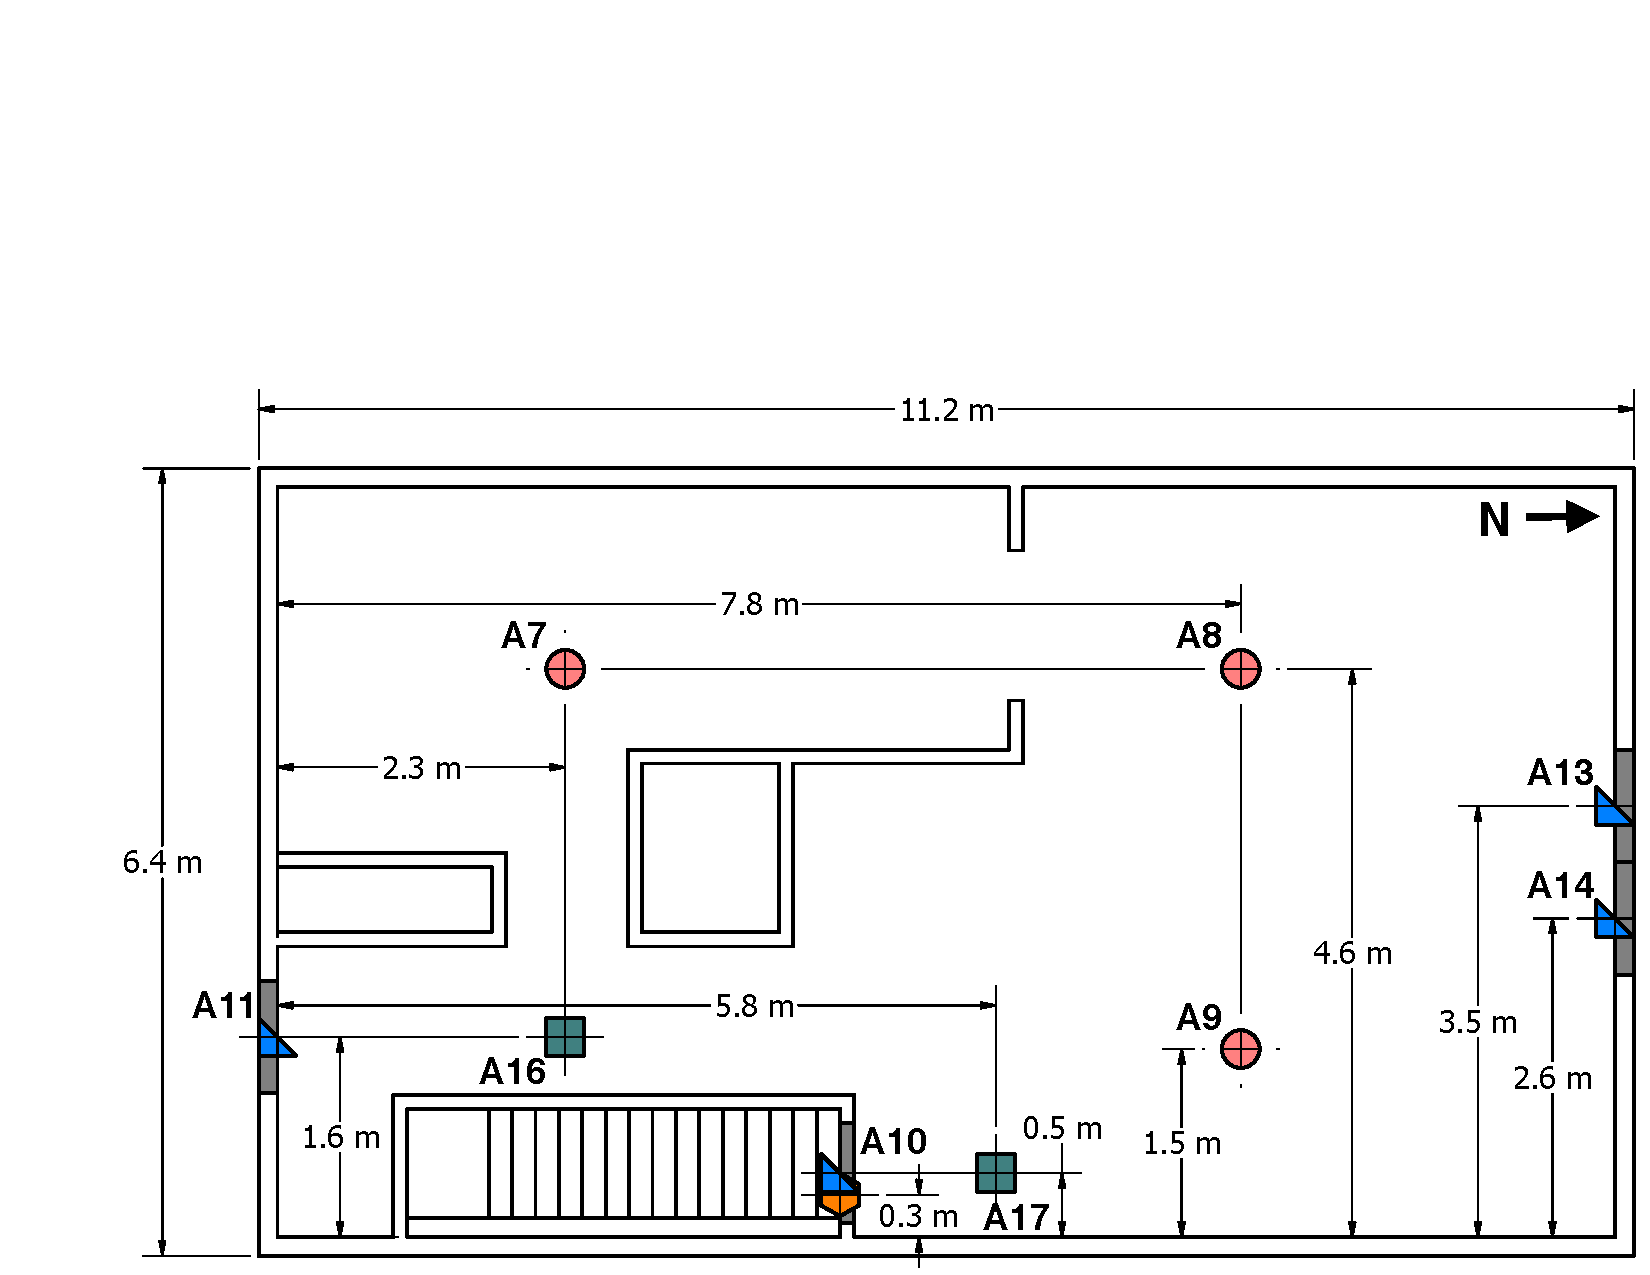
\includegraphics[width=0.94\columnwidth]{Figures/Floor_Plans/West_Structure_2nd_Floor_Dimensioned_Instrumentation}
% 	\\~\\
% 	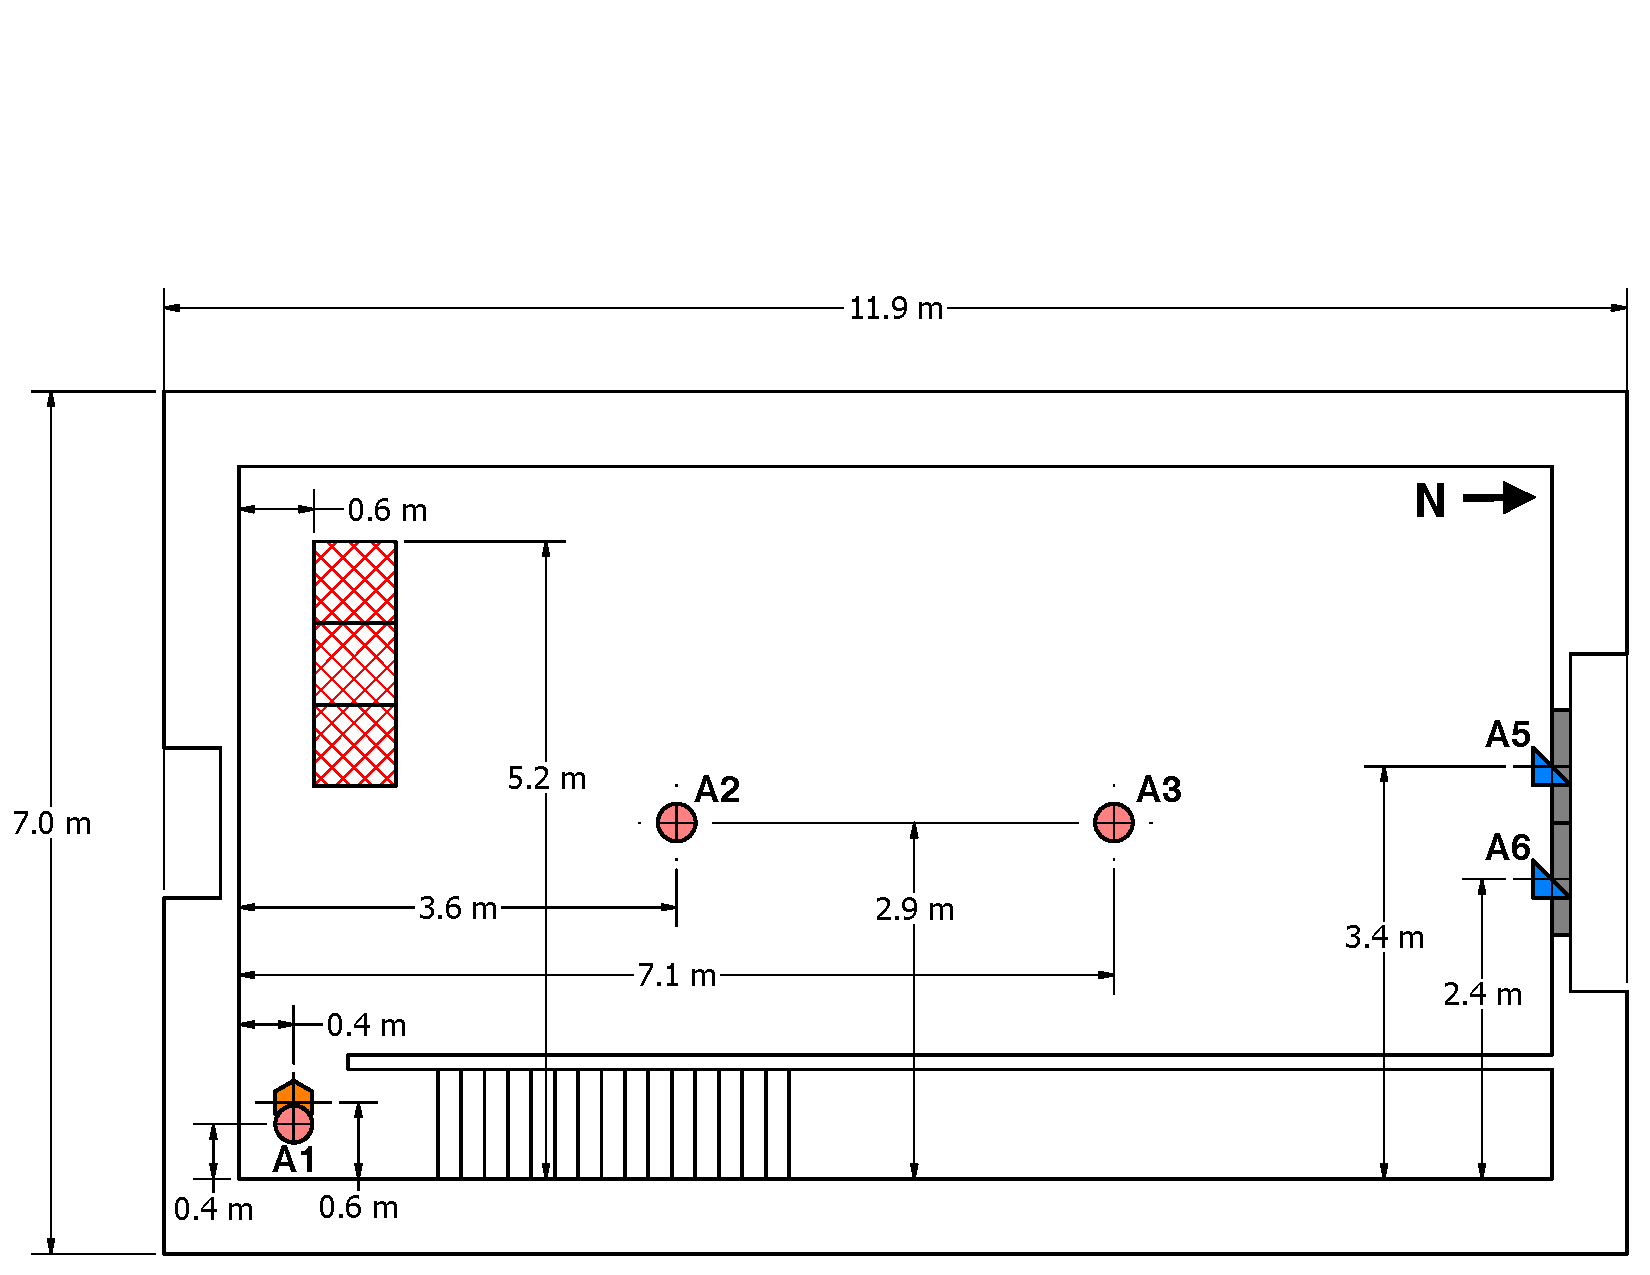
\includegraphics[width=\columnwidth]{Figures/Floor_Plans/West_Structure_1st_Floor_Dimensioned_Instrumentation}
% 	\caption[Locations and labels of instrumentation in the West Structure]{Locations and labels of instrumentation in the second floor (top) and first floor (bottom) of the West Structure.}
% 	\label{fig:west_instrumentation}
% \end{figure}

The thermocouple arrays and bi-directional probe plus solid thermocouple arrays contained eight sensors per array. Gas samples were pulled through 9.5~mm (0.38~in) diameter stainless steel tubing located 1.2~m (4~ft) above the floor. Each pair of total heat flux sensors was located 1.0~m (3.3~ft) above the floor. The pair at A16 contained one sensor facing the ceiling and another facing the north side of the room, and the pair at A17 contained one sensor facing the ceiling and another facing the stairway door. The height of each individual sensor in the sensor arrays is listed in the channel list found in Table~\ref{table:west_channel_list}.
\FloatBarrier

\subsection{Measurement Uncertainty}
This section lists the uncertainties in the reported length, mass, temperature, heat flux, gas species concentration, gas velocity, and heat release rate measurements. Uncertainty estimates are based either on manufacturer literature or analyses performed by others for similar measurement devices and techniques. In accordance with NIST guidelines~\cite{Taylor&Kuyatt:1994}, measurement accuracy is reported as an \textit{expanded uncertainty}, or 95~\% ($2\,\sigma$) confidence interval. Most manufacturer specifications express accuracy in terms of a \textit{standard  uncertainty}, or 68~\% ($1\,\sigma$) confidence interval.

\subsubsection*{\textit{Compartment Dimensions}}
Room dimensions and instrumentation location measurements were made with a hand held laser measurement device with a standard uncertainty of $\pm$6.0~mm (0.25~in) over a range of 0.6~m (2.0~ft) to 15~m (50.0~ft) according to the manufacturer~\cite{StanleyTools}. Steel measuring tapes with a resolution of $\pm$0.5~mm (0.02~in) were used to locate measurement devices. The steel measuring tapes were manufactured in compliance with NIST Manual 44~\cite{Butcher:2012}, which specifies a tolerance of $\pm$1.6~mm (0.06~in) for 9.1~m (30~ft) tapes and $\pm$6.4~mm (0.25~in) for 30.5~m (100~ft) tapes. These uncertainties are all well within the precision of the reported dimensions, which are typically rounded to the nearest 0.1~m.

\subsubsection*{\textit{Thermocouples}}
The standard uncertainty in the temperature of the thermocouple wire itself as stated by the wire manufacturer, OMEGA Engineering, Inc., is $\pm$2.2$~^{\circ}$C at $277~^{\circ}$C and increases to $\pm$9.5$~^{\circ}$C at $871~^{\circ}$C~\cite{Omega:2004}. The variation of the temperature in the environment surrounding the thermocouple is known to be much greater than that of the wire uncertainty. Expanded uncertainties as high as 20~\% for upper layer temperatures measured by a 1~mm bare-bead type K thermocouple have been reported by NIST researchers~\cite{Blevins:1999,Pitts:2003}. Small diameter thermocouples were used during these experiments to limit the impact of radiative heating and cooling. The estimated expanded uncertainty associated with the temperature measurements is $\pm$15~\%.

\subsubsection*{\textit{Heat Flux Gauges}}
Total heat flux measurements were made using water-cooled Schmidt-Boelter gauges. The manufacturer, MEDTHERM Corporation, reports a $\pm$3~\% calibration expanded uncertainty for these devices~\cite{Medtherm:2003}. Results from an international study on total heat flux gauge calibration and response demonstrated that the expanded uncertainty of a Schmidt-Boelter gauge is typically $\pm$8~\%~\cite{Pitts:2006}.

\subsubsection*{\textit{Gas Sampling}}
A gas sampling system from California Analytical Instruments, Inc. (model 602P) with a relative expanded uncertainty of $\pm$1~\% when compared to span gas volume fractions~\cite{Bundy:2007} was used to make gas concentration measurements. However, according to a study by Lock~et~al.~\cite{Lock:1}, the non-uniformity and movement of exhaust gases contribute to an estimated expanded uncertainty of $\pm$12~\%.

\subsubsection*{\textit{Bi-Directional Probes}}
Bi-directional probes with Setra 264 pressure transducers from Setra Systems, Inc. were used to measure gas velocity through doorways. An expanded uncertainty ranging from $\pm$14~\% to $\pm$22~\% for bi-directional probes of similar design was calculated by Bryant of NIST~\cite{Bryant:FSJ2009}.

\subsubsection*{\textit{Heat Release Rate}}
A positive displacement rotary gas meter was used to measure the volume flow rate of propane into the gas burners. The manufacturer, Romet Limited, reports a relative standard uncertainty of $\pm$2~\% for this type of meter (model RM-3000)~\cite{Romet:2014}. A volumetric flow rate was calculated from the gas meter volume readings and used in conjunction with the heat of combustion of propane to calculate the heat release rate of the fire for each experiment. The total expanded uncertainty for the heat release rate obtained from this method is estimated to be $\pm8$~\%.
%%%%%%%%%%%%%%%%%%%%%%%%%%%%%%%%%%%%%
% CHAPTER 3: Experimental Procedure %
%%%%%%%%%%%%%%%%%%%%%%%%%%%%%%%%%%%%%
%................................
% Notes about things to add/edit 
%................................
% >> Determine best way to present the Fig+Table combinations
% >> Add test matrix
% 		* Items: Test Name, Structure, Description 
% 		* Potential additions: ramp or instant? Multiple seqs? PPV? 
% 				Duration? Variation of parameters? Ambient Temp?
% 				Open Vents?
% >> Text alignment after double digit numbers in event time tables
%%%%%%%%%%%%%%%%%%%%%%%%%%%%%%%%%%%%%%%%%%%%%%%%%%%%%%%%%%%%%%%%%%%%%

\renewcommand{\thechapter}{3}

\chapter{Experimental Procedure}
\label{chap:exp_procedure}

A similar procedure was followed for all nine propane gas burner experiments described in this report. First, the three propane burners were ignited in sequential order. Next, various doors and vents were opened and closed to change the ventilation pattern in the structure. Then, the burners were turned off, extinguishing the fire. After the burners were extinguished, data continued to be collected while different doors and vents were opened to cool the interior of the structure. A positive pressure ventilation (PPV) fan was used during some tests to expedite the cooling of the structure. 

The nine propane gas burner tests were conducted in series with a variety of other experiments. In order to be consistent with the original test numbering, the gas burner experiments described in this report are referred to as Tests~2--6 and Tests~22--25. The experiments and their different parameters are summarized in Table~\ref{table:exp_summary} below.

\renewcommand{\baselinestretch}{1}
\begin{sidewaystable}[!ht]
\begin{center}
\caption{Summary of Propane Gas Burner Experiments.}
\begin{tabular}{ccccl}
\toprule
% \multirow{2}{*}{Test~\#}    
\textbf{Name}  	& 	\textbf{Structure} 	& 	\textbf{Duration of Fire} 	& 	\textbf{Heat Release Rate} 	& 	\multicolumn{1}{c}{\textbf{Ventilation}}	\\ 
				& 						& 		\textbf{(min:sec)} 		& 	\textbf{Rate (kW)}			& 													\\
\midrule
Test 2 			& 	East 				&  		16:01 					& 	N.R.$^*$ 					& 	Both double doors, south door, PPV after fire	\\
Test 3			& 	East 				&  		16:58 					&   N.R.$^*$   					& 	Both double doors, south door, PPV after fire					\\
Test 4			& 	East 				&  		16:59 					&  	N.R.$^*$ 					& 	Both double doors, south door, PPV after fire					\\
\multicolumn{5}{c}{} \\
Test 5 			& 	East 				&  		 9:36 					&  		1190 					& 	Roof vent, both double doors				 					\\
				& 						& 		10:15 					&  		1190 					& 	Roof vent, both double doors				 					\\
				& 						& 		 9:32 					&  		1190 					& 	Roof vent, both double doors				 					\\				
\multicolumn{5}{c}{} \\
Test 6			&	East 				&  		 5:27 					&  		1190 					& 	Roof vent, west double door					 	    			\\
				& 						& 		 5:03 					&  		1190 					& 	Roof vent, west double door					 	    			\\
				& 						& 		 5:12 					&  		1180 					& 	Roof vent, west double door					 	    			\\
\multicolumn{5}{c}{} \\
Test 22			&	West 				&  		16:58 					&  		1240 					& 	Both sets of double doors, 2nd floor south door, PPV fan 		\\
Test 23			&	West 				&  		16:58 					&  		1290 					& 	Both sets of double doors, PPV fan						 		\\
Test 24			&	West 				&  		16:58 					&  		1270 					&   West double door on both floors, 2nd floor south door, PPV fan 	\\
Test 25			&	West 				&  		16:58 					&  		1270 					& 	West double door on both floors, 2nd floor south door, PPV fan 	\\
\bottomrule
\multicolumn{5}{l}{$^*$\footnotesize{Not reported because propane flow rate was not accurately measured during tests}}
\end{tabular}
\end{center}
% $^1$ \footnotesize Not reported because propane flow rate could not be accurately measured during tests
\label{table:exp_summary}
\end{sidewaystable}
\clearpage
% FloatBarrier

\section{East Structure Tests}
Five different tests, Tests~2--6, were conducted in the East Structure. Table~\ref{table:HRR_Tests_5-6} lists the heat release rates for Tests~5 and 6. The time between the ignition of each gas burner for Tests~5 and 6 was on the order of seconds. As a result, a single heat release rate, one for all three burners ignited, is reported.

\renewcommand{\baselinestretch}{1}
% \begin{table}[h]
% \caption[Heat Release Rates for Tests~5 and 6.]{Heat Release Rates (kW) for Tests~5 and 6.}
% \begin{center}
% \begin{tabular}{|c|c|}
% \hline
%  % & \textbf{Heat Release Rate (kW)} \\
% \multirow{2}{*}{Test~\#}    & Heat Release Rate for \\ 
% 							& all Burners Ignited (kW) \\
% \hline \hline
% 5 -- Seq. 1		& 1190 \\
% 5 -- Seq. 2		& 1190 \\
% 5 -- Seq. 3		& 1190 \\
% 6 -- Seq. 1		& 1190 \\
% 6 -- Seq. 2		& 1190 \\
% 6 -- Seq. 3		& 1180 \\
% \hline
% \end{tabular}
% \end{center}
% \label{table:HRR_Tests_5-6}
% \end{table}

\begin{table}[!ht]
\caption[Heat Release Rates for Tests~5 and 6.]{Heat Release Rates for Tests~5 and 6.}
\begin{center}
\begin{tabular}{lc}
 \toprule
 & \textbf{Heat Release Rate (kW)} \\
\textbf{Test} & \textbf{All Burners On} \\
\midrule
Test 5 - Seq. 1		& 1190 \\
Test 5 - Seq. 2		& 1190 \\
Test 5 - Seq. 3		& 1190 \\
Test 6 - Seq. 1		& 1190 \\
Test 6 - Seq. 2		& 1190 \\
Test 6 - Seq. 3		& 1180 \\
\bottomrule
\end{tabular}
\end{center}
\label{table:HRR_Tests_5-6}
\end{table}
\FloatBarrier

\subsection{Tests 2--4}
Tests~2--4 followed a nearly identical order of events. Figure~\ref{fig:Tests_2-4_layout} includes a schematic floor plan and table of event times corresponding to the data files for each test. A 0.61~cm (2.0~ft) diameter PPV fan located 1.6~m (5.2~ft) away from the south exterior door was aimed at the center of the doorway and used after all burners were extinguished. During Tests~2--4, the south exterior door was not able to completely close due to an obstruction caused by the hoses used to transport the propane to the burners. So, when the south door was in the ``closed'' position, a 133~mm (5.25~in) opening was present between the door and its frame. For all other experiments, however, the south exterior door was not used and the doorway remained closed for the entirety of the test. To fully close the doorway during these tests, the hinged door was removed and replaced by a piece of gypsum board that completely covered the doorway.
\\
\begin{figure}[!ht]
\renewcommand{\baselinestretch}{1}
\begin{minipage}[b]{1.01\columnwidth}
\begin{center}
	% \begin{flushleft}
	\begin{tabular}{lccc}
	\multicolumn{4}{c}{\normalsize Event Times (sec) for Tests~2--4 Data Files} \\
	\toprule
	\multicolumn{1}{c}{\textbf{Event}} 	& \textbf{Test 2} & \textbf{Test 3} & \textbf{Test 4} \\
	\midrule
	~(1)~ Corner burner on 				& 	0		  	  &	 	0			&		0		  \\
	~(2)~ Middle burner on 				&   181			  &		181			&		179		  \\
	~(3)~ Center burner on 				&   361			  &	   	361			&	   	360		  \\
	~(4)~ West double door opened 		&   418			  &    	416			&	   	415		  \\
	~(5)~ East double door opened 		&   538			  &    	536			&	   	535		  \\
	~(6)~ South exterior door opened 	&   604			  &    	597			&	   	597		  \\
	~(7)~ Center burner off				&   720			  &    	778			&	   	778		  \\
	~(8)~ Middle burner off				&   840			  &    	898			&	   	897		  \\
	~(9)~ Corner burner off				&   961			  &    	1018		&	   	1019	  \\
	(10) PPV fan on 					& 	1256		  &    	1316		&  	   	1319	  \\
	(11) PPV fan off 					& 	1892 		  & 	N/A 		& 		1380	  \\
	(12) PPV fan on 					& 	N/A 		  & 	N/A 		& 		1487 	  \\
	\bottomrule
	\end{tabular}
	% \end{flushleft}
	% \begin{tabular}{|l|c|c|c|}
	% \multicolumn{4}{c}{Event Times (sec) for Tests~2--4 Data Files}
	% \vspace{5pt} \\
	% \hline
	% \multicolumn{1}{|c|}{Event}		    & Test 2 		  & Test 3 			& Test 4 \\
	% \hline \hline
	% ~(1)~ Corner burner on 				& 	0		  	  &	 	0			&		0		  \\
	% ~(2)~ Middle burner on 				&   181			  &		181			&		179		  \\
	% ~(3)~ Center burner on 				&   361			  &	   	361			&	   	360		  \\
	% ~(4)~ West double door opened 		&   418			  &    	416			&	   	415		  \\
	% ~(5)~ East double door opened 		&   538			  &    	536			&	   	535		  \\
	% ~(6)~ South exterior door opened 	&   604			  &    	597			&	   	597		  \\
	% ~(7)~ Center burner off				&   720			  &    	778			&	   	778		  \\
	% ~(8)~ Middle burner off				&   840			  &    	898			&	   	897		  \\
	% ~(9)~ Corner burner off				&   961			  &    	1018		&	   	1019	  \\
	% (10) PPV fan on 					& 	1256		  &    	1316		&  	   	1319	  \\
	% (11) PPV fan off 					& 	1892 		  & 	N/A 		& 		1380	  \\
	% (12) PPV fan on 					& 	N/A 		  & 	N/A 		& 		1487 	  \\
	% \hline
	% \end{tabular}
\end{center}
\end{minipage}
\begin{minipage}[b]{0.9\columnwidth}
	\vspace{20pt}
	\centering
	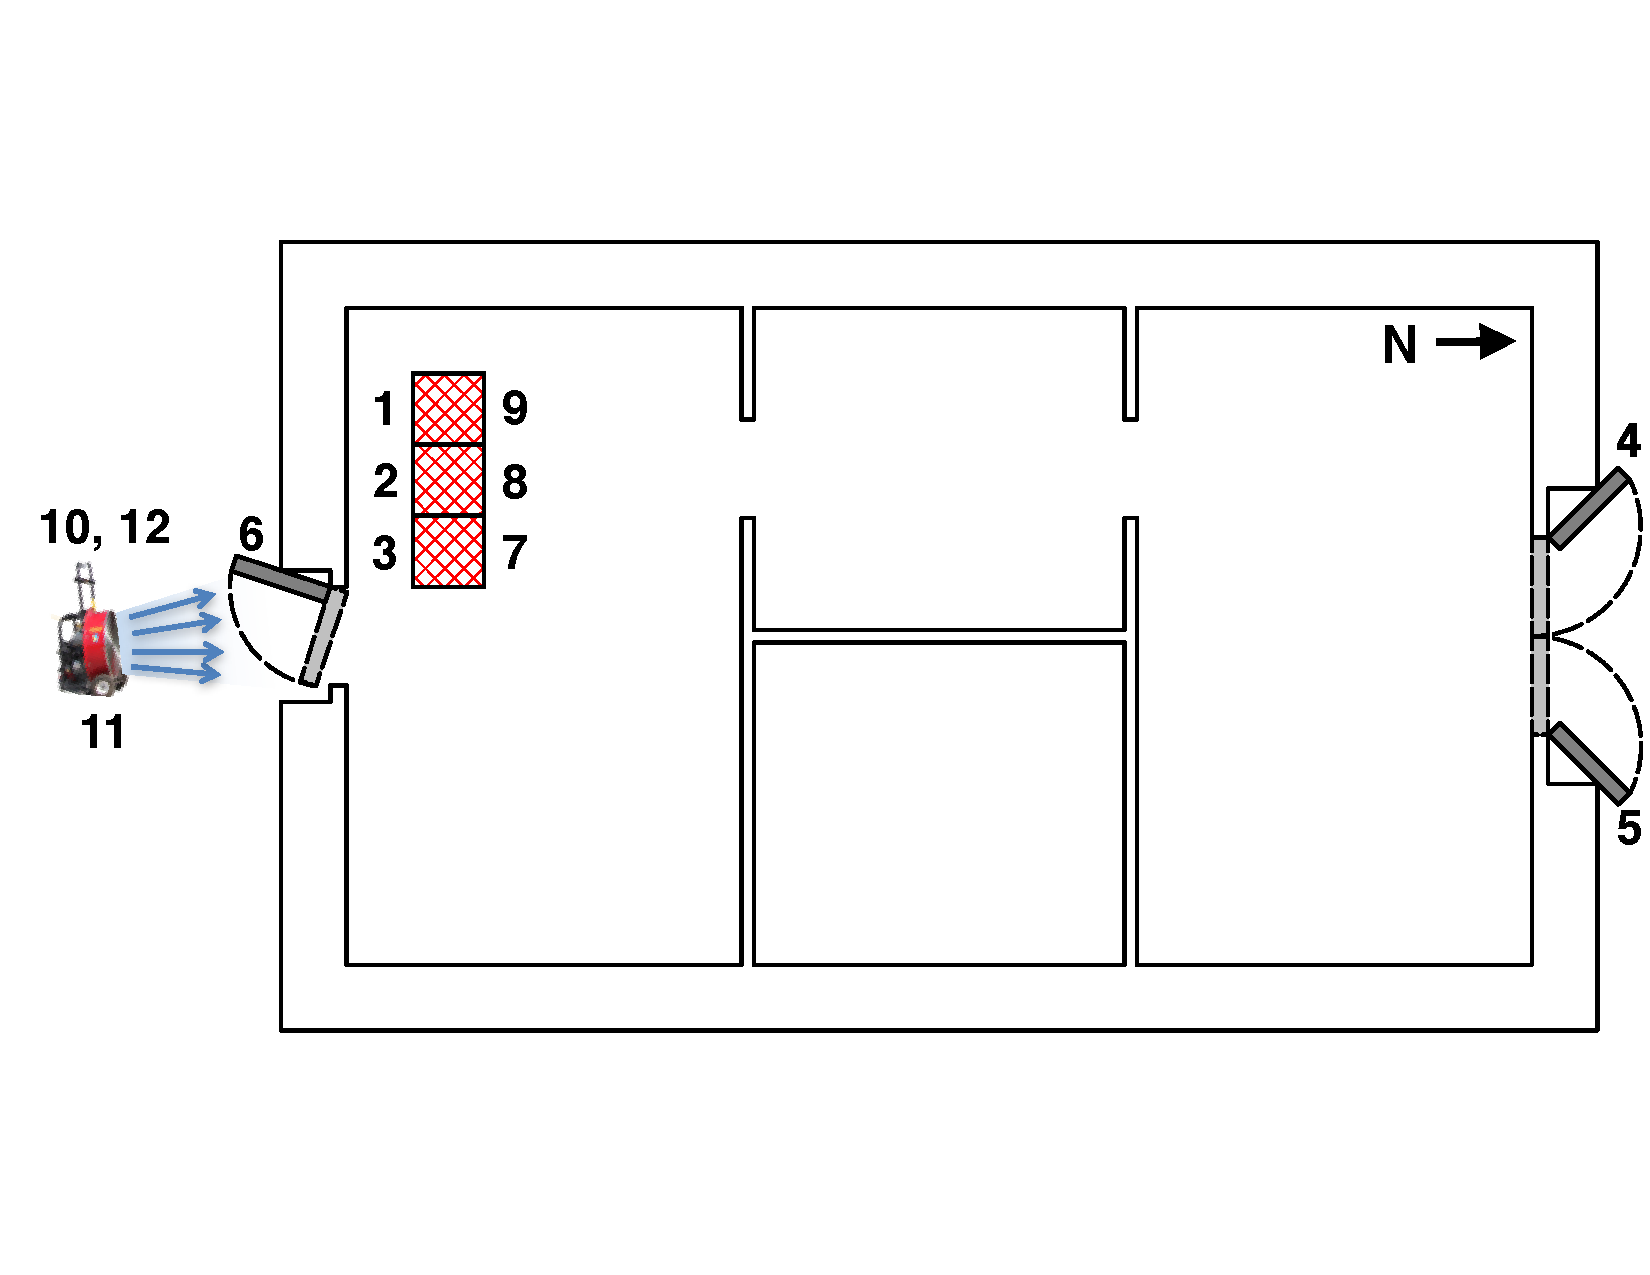
\includegraphics[width=\columnwidth]{Figures/Floor_Plans/East_Structure_Test_4}
\end{minipage}
\renewcommand{\baselinestretch}{1}
\caption{Tests~2--4 layout and event times.}
\label{fig:Tests_2-4_layout}
\end{figure}
\FloatBarrier

\subsection{Tests 5 \& 6}
The procedures for Tests~5 and 6 are outlined in Figures~\ref{fig:east_test_5} and \ref{fig:east_test_6}, respectively. Both tests involved repeating a specific set of events three times in a row. To avoid listing the identical actions three separate times in the ``event'' column of the tables, each repetition of events is denoted as a ``sequence'' (abbreviated as ``seq.''), and each table contains three columns of times --- one for each sequence.
\\
% \begin{figure}[!ht]
% \begin{minipage}[b]{0.8\columnwidth}
% 	\begin{flushleft}
% 	\begin{tabular}{lccc}
% 	\multicolumn{4}{c}{\normalsize Event Times (s) for Test~5 Data File} \\
% 	\toprule
% 	\multicolumn{1}{c}{\textbf{Event}} 	& \textbf{Seq. 1} & \textbf{Seq. 2} & \textbf{Seq. 3} \\
% 	\midrule
% 	~(1)~ All burners on 				& 	0			  &	   1225			&	   2425		\\
% 	~(2)~ Roof vent opened 				&   154			  &    1345			&	   2545		\\
% 	~(3)~ West double door opened 		&	175			  &	   1432	 		&	   2632 	\\
% 	~(4)~ East double door opened 		&   361			  &    1524			&	   2730		\\
% 	~(5)~ Roof vent closed		 		&   445			  &    1723			&	   2852		\\
% 	~(6)~ All burners off 				&   576			  &    1840			&	   2997		\\
% 	~(7)~ Roof vent opened				& 	720 		  &	   1890			&	   3086		\\
% 	~(8)~ East double door closed		& 	1148 		  &	   2311			&	   N/A		\\
% 	~(9)~ West double door closed		& 	1164 		  &	   2330			&	   N/A		\\
% 	(10) Roof vent closed		 		&   1179		  &    2387			&	   N/A		\\
% 	\bottomrule
% 	\end{tabular}
% 	\end{flushleft}
% \end{minipage}
% \begin{minipage}[b]{0.9\columnwidth}
% 	\vspace{15pt}
% 	\centering
% 	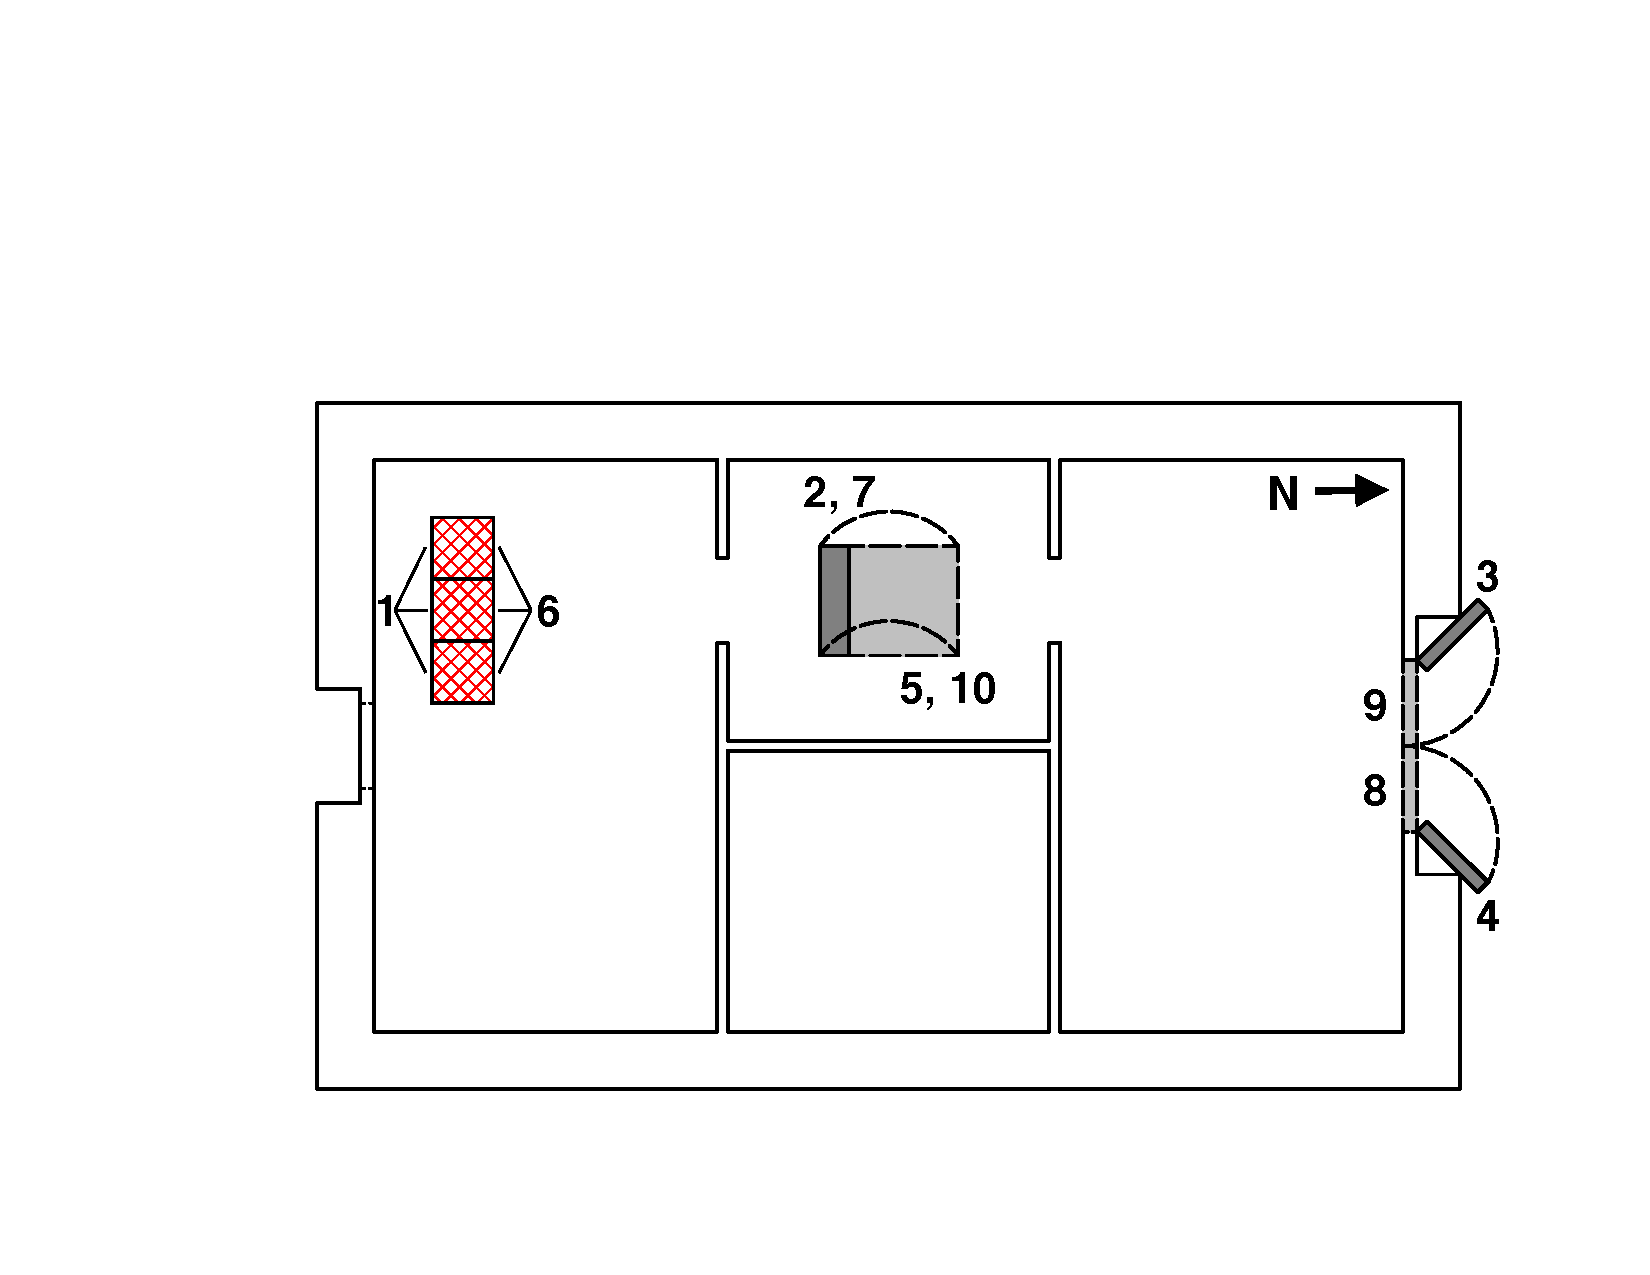
\includegraphics[width=0.86\columnwidth]{Figures/Floor_Plans/East_Structure_Test_5}
% \end{minipage}
% \caption{Test~5 layout and event times.}
% \label{fig:east_test_5}
% \end{figure}
% \clearpage

\begin{figure}[!ht]
\renewcommand{\baselinestretch}{1}
\begin{minipage}[b]{0.96\columnwidth}
\begin{center}
	\begin{tabular}{lccc}
	\multicolumn{4}{c}{\normalsize Event Times (sec) for Test~5 Data File} \\
	\toprule
	\multicolumn{1}{c}{\textbf{Event}} 	& \textbf{Seq. 1} & \textbf{Seq. 2} & \textbf{Seq. 3} \\
	\midrule
	~(1)~ All burners on 				& 	0			  &	   1225			&	   2425		\\
	~(2)~ Roof vent opened 				&   154			  &    1345			&	   2545		\\
	~(3)~ West double door opened 		&	175			  &	   1432	 		&	   2632 	\\
	~(4)~ East double door opened 		&   361			  &    1524			&	   2730		\\
	~(5)~ Roof vent closed		 		&   445			  &    1723			&	   2852		\\
	~(6)~ All burners off 				&   576			  &    1840			&	   2997		\\
	~(7)~ Roof vent opened				& 	720 		  &	   1890			&	   3086		\\
	~(8)~ East double door closed		& 	1148 		  &	   2311			&	   N/A		\\
	~(9)~ West double door closed		& 	1164 		  &	   2330			&	   N/A		\\
	(10) Roof vent closed		 		&   1179		  &    2387			&	   N/A		\\
	\bottomrule
	\end{tabular}
	% \begin{tabular}{|l|c|c|c|}
	% \multicolumn{4}{c}{Event Times (sec) for Test~5 Data File}
	% \vspace{5pt} \\
	% \hline
	% \multicolumn{1}{|c|}{Event}		    & Seq. 1 		  & Seq. 2 			& 	Seq. 3 \\
	% \hline \hline
	% ~(1)~ All burners on 				& 	0			  &	   1225			&	   2425		\\
	% ~(2)~ Roof vent opened 				&   154			  &    1345			&	   2545		\\
	% ~(3)~ West double door opened 		&	175			  &	   1432	 		&	   2632 	\\
	% ~(4)~ East double door opened 		&   361			  &    1524			&	   2730		\\
	% ~(5)~ Roof vent closed		 		&   445			  &    1723			&	   2852		\\
	% ~(6)~ All burners off 				&   576			  &    1840			&	   2997		\\
	% ~(7)~ Roof vent opened				& 	720 		  &	   1890			&	   3086		\\
	% ~(8)~ East double door closed		& 	1148 		  &	   2311			&	   N/A		\\
	% ~(9)~ West double door closed		& 	1164 		  &	   2330			&	   N/A		\\
	% (10)~ Roof vent closed		 		&   1179		  &    2387			&	   N/A		\\
	% \hline
	% \end{tabular}
\end{center}
\end{minipage}
\begin{minipage}[b]{\columnwidth}
	\vspace{20pt}
	\centering
	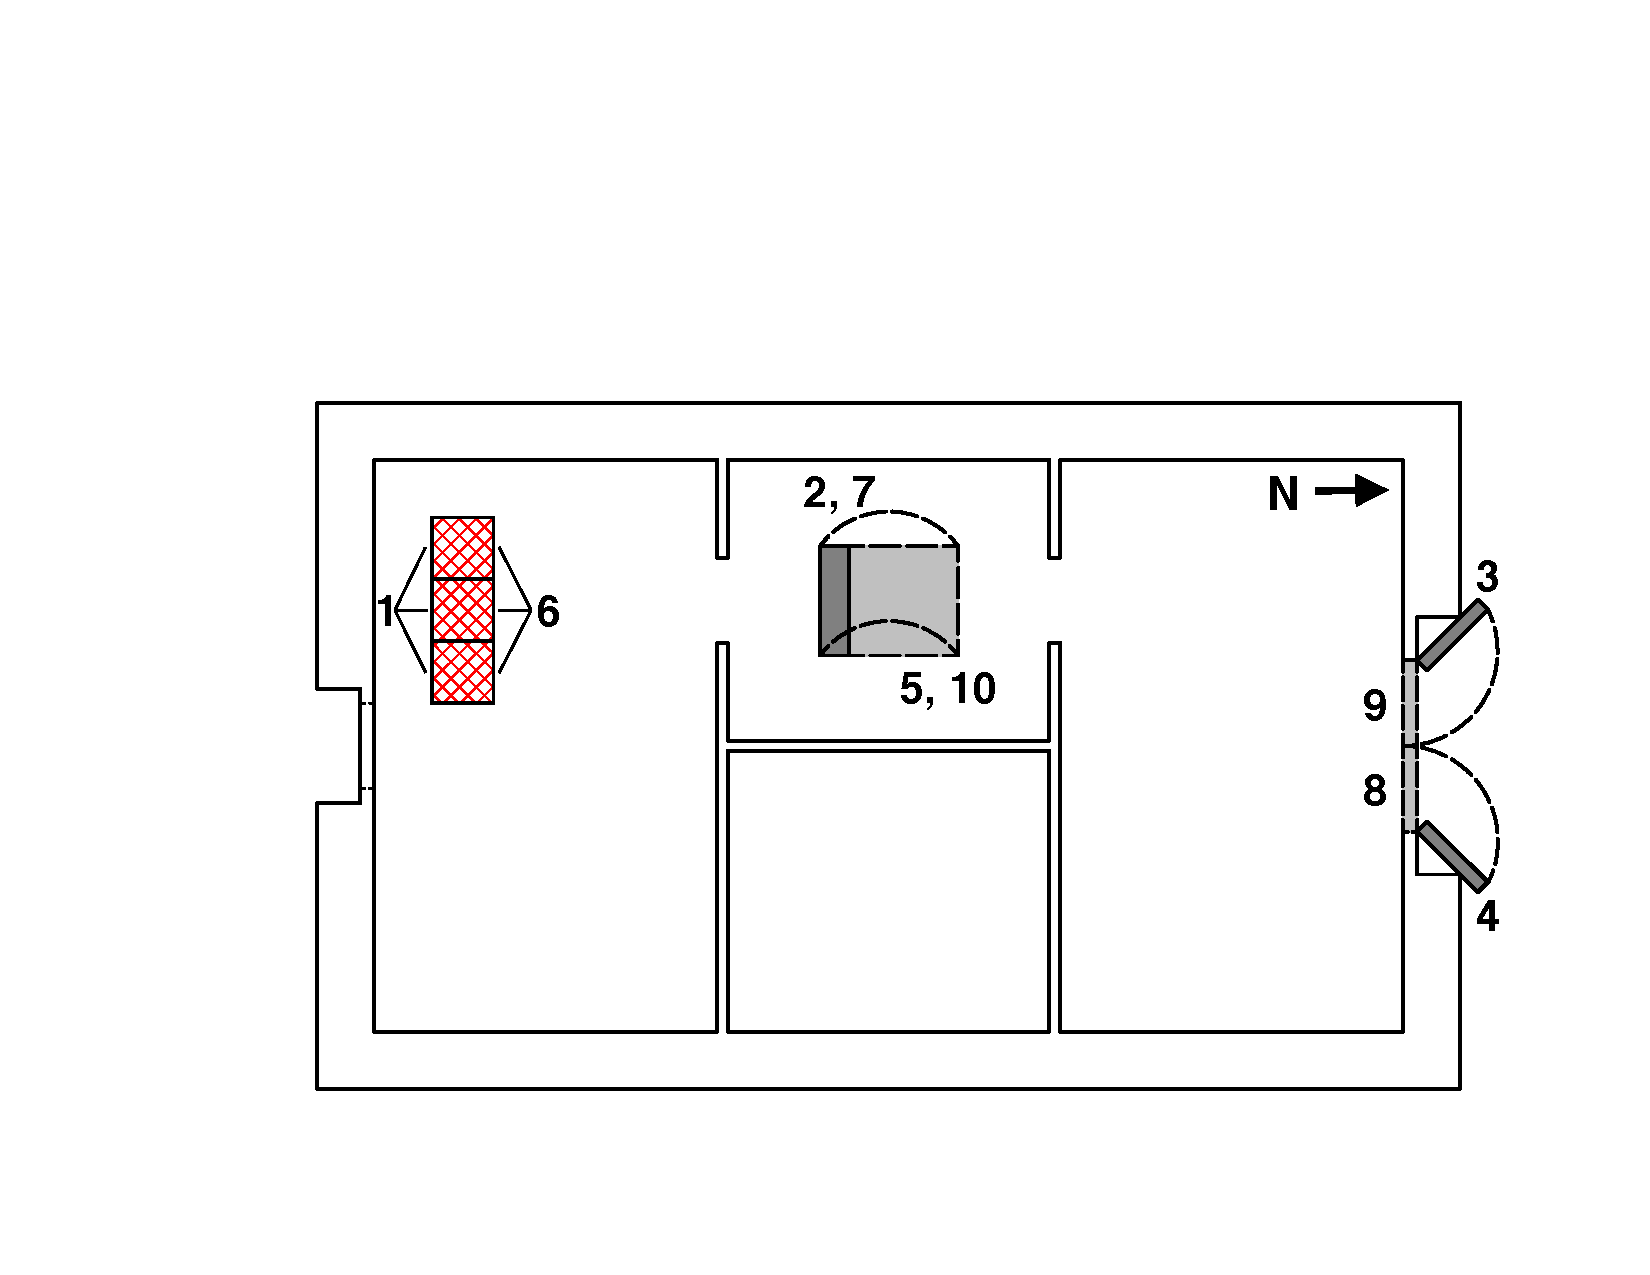
\includegraphics[width=0.76\columnwidth]{Figures/Floor_Plans/East_Structure_Test_5}
\end{minipage}
\renewcommand{\baselinestretch}{1}
\caption{Test~5 layout and event times.}
\label{fig:east_test_5}
\end{figure}
\FloatBarrier

% \begin{figure}[!ht]
% \begin{minipage}[b]{0.8\columnwidth}
% 	\begin{flushleft}
% 	\begin{tabular}{lccc}
% 	\multicolumn{4}{c}{\normalsize Event Times (s) for Test~6 Data File} \\
% 	\toprule
% 	\multicolumn{1}{c}{\textbf{Event}} 	& \textbf{Seq. 1}	& \textbf{Seq. 2} 	& \textbf{Seq. 3} 	\\
% 	\midrule
% 	~(1)~ All burners on 				&	0				&	565				&	1075			\\
% 	~(2)~ West double door opened 		&	116				&   685				&	1195			\\
% 	~(3)~ Roof vent opened 		    	&	207				&	747 			& 	1287 			\\
% 	~(4)~ All burners off 				&	327				&   868				&	1387			\\
% 	~(5)~ East double door opened		&	369				&   911				&	1446			\\
% 	~(6)~ Roof vent closed 				&	494				&   1040			&	N/A				\\
% 	~(7)~ East double door closed		&	522 			&	1012			&	N/A 			\\
% 	~(8)~ West double door closed		&	538 			&	1025			&	N/A				\\
% 	\bottomrule
% 	\end{tabular}
% 	\end{flushleft}
% \end{minipage}
% \begin{minipage}[b]{0.86\columnwidth}
% 	\vspace{15pt}
% 	\centering
% 	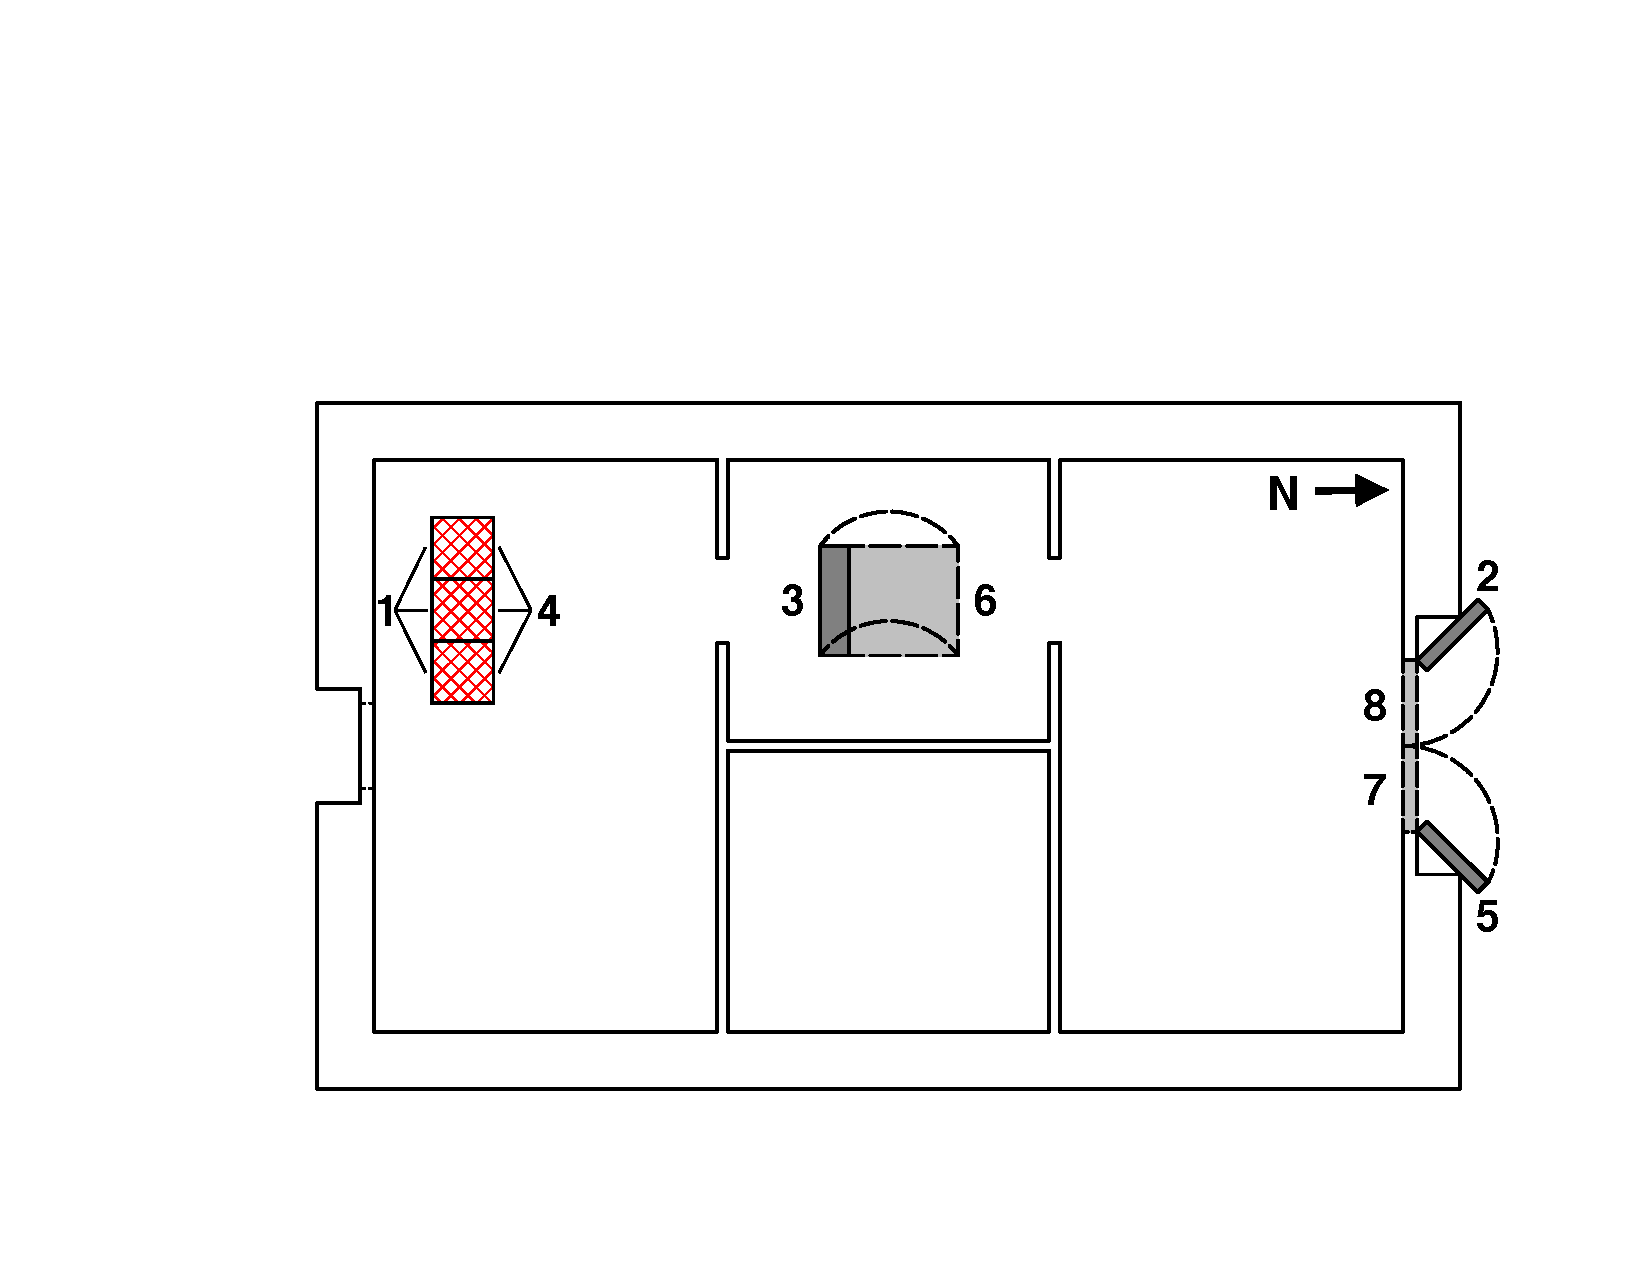
\includegraphics[width=\columnwidth]{Figures/Floor_Plans/East_Structure_Test_6}
% \end{minipage}
% \caption{Test~6 layout and event times.}
% \label{fig:east_test_6}
% \end{figure}
% \clearpage
% \renewcommand{\baselinestretch}{2}

\begin{figure}[!ht]
\renewcommand{\baselinestretch}{1}
\begin{minipage}[b]{0.98\columnwidth}
\begin{center}
	\begin{tabular}{lccc}
	\multicolumn{4}{c}{\normalsize Event Times (sec) for Test~6 Data File} \\
	\toprule
	\multicolumn{1}{c}{\textbf{Event}} 	& \textbf{Seq. 1}	& \textbf{Seq. 2} 	& \textbf{Seq. 3} 	\\
	\midrule
	~(1)~ All burners on 				&	0				&	565				&	1075			\\
	~(2)~ West double door opened 		&	116				&   685				&	1195			\\
	~(3)~ Roof vent opened 		    	&	207				&	747 			& 	1287 			\\
	~(4)~ All burners off 				&	327				&   868				&	1387			\\
	~(5)~ East double door opened		&	369				&   911				&	1446			\\
	~(6)~ Roof vent closed 				&	494				&   1040			&	N/A				\\
	~(7)~ East double door closed		&	522 			&	1012			&	N/A 			\\
	~(8)~ West double door closed		&	538 			&	1025			&	N/A				\\
	\bottomrule
	\end{tabular}
	% \begin{tabular}{|l|c|c|c|}
	% \multicolumn{4}{c}{Event Times (sec) for Test~6 Data File}
	% \vspace{5pt} \\
	% \hline
	% \multicolumn{1}{|c|}{Event}		    & Seq. 1 		  	& Seq. 2 			& 	Seq. 3 			\\
	% \hline \hline
	% ~(1)~ All burners on 				&	0				&	565				&	1075			\\
	% ~(2)~ West double door opened 		&	116				&   685				&	1195			\\
	% ~(3)~ Roof vent opened 		    	&	207				&	747 			& 	1287 			\\
	% ~(4)~ All burners off 				&	327				&   868				&	1387			\\
	% ~(5)~ East double door opened		&	369				&   911				&	1446			\\
	% ~(6)~ Roof vent closed 				&	494				&   1040			&	N/A				\\
	% ~(7)~ East double door closed		&	522 			&	1012			&	N/A 			\\
	% ~(8)~ West double door closed		&	538 			&	1025			&	N/A				\\
	% \hline
	% \end{tabular}
\end{center}
\end{minipage}
\begin{minipage}[b]{\columnwidth}
	\vspace{20pt}
	\centering
	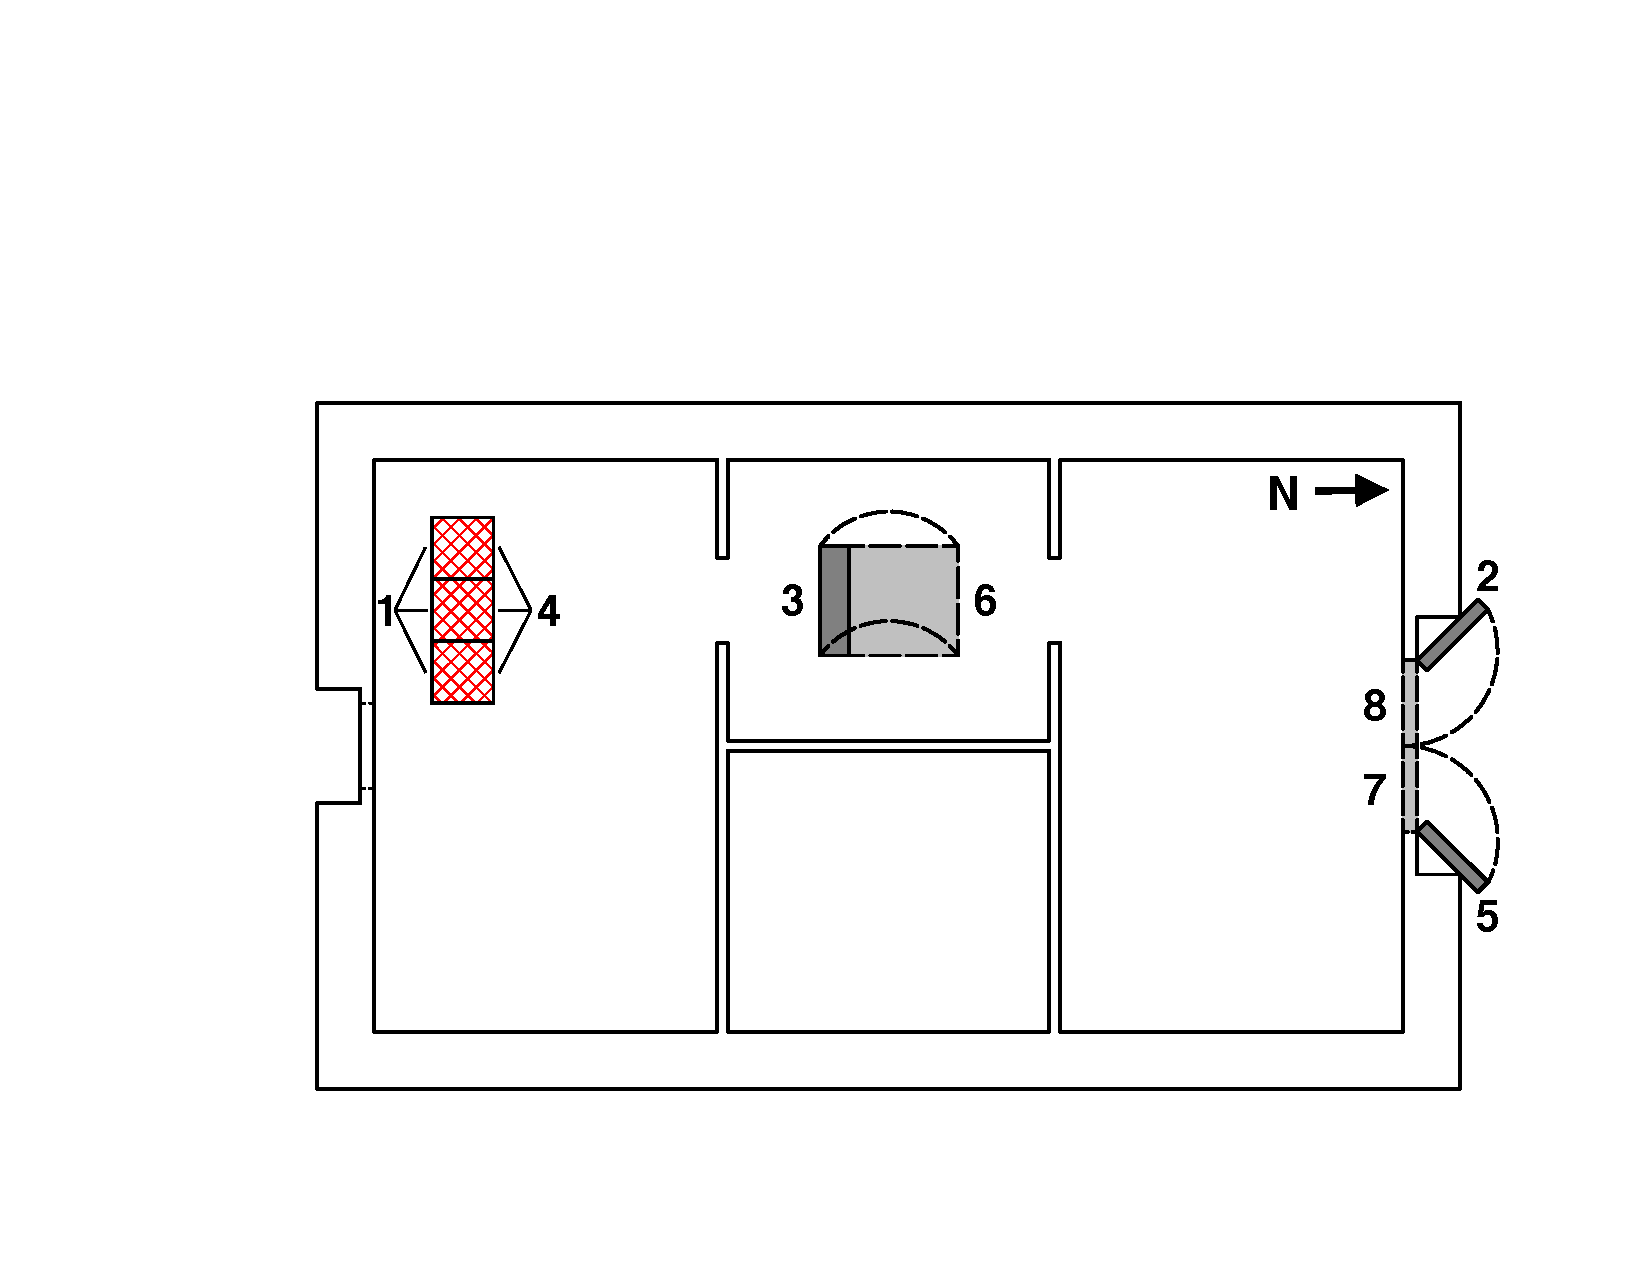
\includegraphics[width=0.8\columnwidth]{Figures/Floor_Plans/East_Structure_Test_6}
\end{minipage}
\renewcommand{\baselinestretch}{1}
\caption{Test~6 layout and event times.}
\label{fig:east_test_6}
\end{figure}
\FloatBarrier

\section{West Structure Tests}

Four of the gas burner experiments, Tests~22--25, were conducted in the West Structure. Table~\ref{table:HRR_Tests_22-25} lists the calculated heat release rate for each test. Similar to Tests~5 and 6, Tests~22--25 had a duration on the order of seconds between the ignition of each burner, so only the heat release rate for all three burners is reported.

\renewcommand{\baselinestretch}{1}
% \begin{table}[h]
% \caption[Heat Release Rates for Tests~22--25.]{Heat Release Rates (kW) for Tests~22--25.}
% \begin{center}
% \begin{tabular}{|c|c|}
% \hline
%  % & \textbf{Heat Release Rate (kW)} \\
% \multirow{2}{*}{Test~\#}    & Heat Release Rate for \\ 
% 							& All Burners Ignited (kW) \\
% \hline \hline
% 22				&     	1240 	  \\
% 23				&     	1290 	  \\
% 24				& 	    1270 	  \\
% 25				&     	1270 	  \\
% \hline
% \end{tabular}
% \end{center}
% \label{table:HRR_Tests_22-25}
% \end{table}
% \renewcommand{\baselinestretch}{2}
\begin{table}[!ht]
\caption{Heat Release Rates for Tests~22--25.}
\begin{center}
\begin{tabular}{lc}
 \toprule
					& 	\textbf{Heat Release Rate (kW)}	\\
\textbf{Test}		& 	\textbf{All Burners On} \\
 \midrule
Test 22				&     	1240 	  \\
Test 23				&     	1290 	  \\
Test 24				& 	    1270 	  \\
Test 25				&     	1270 	  \\
\bottomrule
\end{tabular}
\end{center}
\label{table:HRR_Tests_22-25}
\end{table}
% \renewcommand{\baselinestretch}{2}
\FloatBarrier
\subsection{Tests~22 \& 23}

Tests~22 and 23 followed nearly identical procedures. The starting configuration for Test~22 had the second-story, south exterior door in the opened position, while the starting configuration for Test~23 had the same door in the closed position. Figure~\ref{fig:west_test_22} includes a floor plan schematic and table of event times corresponding to the data files for Tests~22 and 23. A 0.61~m (2.0~ft) diameter PPV fan located 2.3~m (7.5~ft) away from the first level double doors and aimed at the center of the two doors was used towards the end of both tests.
% \begin{figure}[!ht]
% \begin{minipage}[b]{0.8\columnwidth}
% 	\begin{flushleft}
% 	\begin{tabular}{lcc}
% 	\multicolumn{3}{c}{Event Times (s) for Tests~22--23 Data Files} \\
% 	\toprule
% 	\multicolumn{1}{c}{\textbf{Event}} 			& \textbf{Test 22}	& \textbf{Test 23} \\
% 	\midrule
% 	~(1)~  All burners on 						&   0	  			&	 0			\\
% 	~(2)~  2nd floor west double door opened 	&   194		  		&    130		\\
% 	~(3)~  1st floor west double door opened 	&	314		  		&    252 	 	\\
% 	~(4)~  1st floor east double door opened 	&   450			  	&    371		\\
% 	~(5)~  2nd floor south exterior door closed &   511		  		&    N/A		\\
% 	~(6)~  2nd floor east double door opened	&   585			  	&    498		\\
% 	~(7)~  PPV fan on 							&   652			  	&    612		\\
% 	~(8)~  PPV fan off              			&   798			  	&    761		\\
% 	~(9)~  All burners off 						&   829			  	&    794		\\
% 	(10)   2nd floor south exterior door opened &   899			  	&    849		\\
% 	(11)   PPV fan on 	 						&   1065		  	&    940		\\
% 	(12)   2nd floor south exterior door closed &   1176		  	&    N/A		\\
% 	\bottomrule
% 	\end{tabular}
% 	\end{flushleft}
% \end{minipage}
% \begin{minipage}[b]{0.9\columnwidth}
% 	\vspace{15pt}
% 	\centering
% 	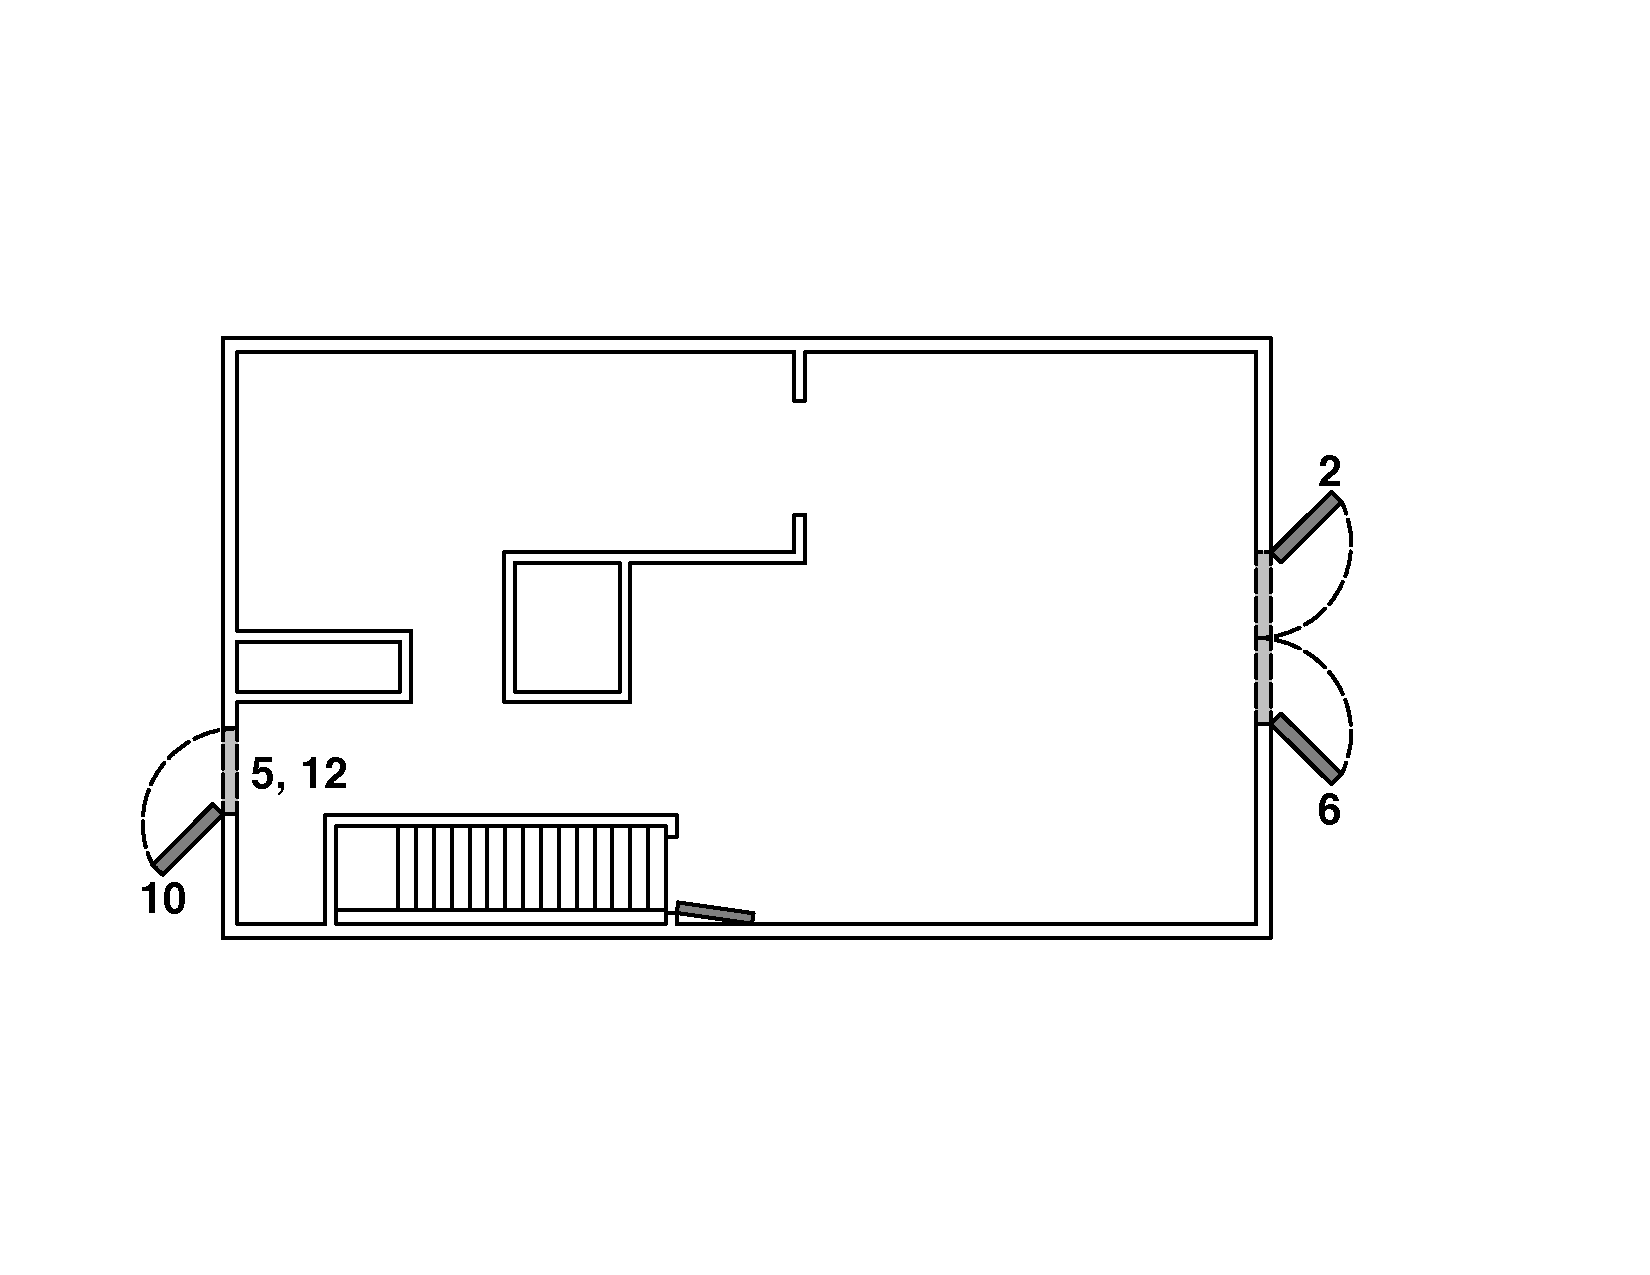
\includegraphics[width=\columnwidth]{Figures/Floor_Plans/West_Structure_2nd_Floor_Test_22}
% 	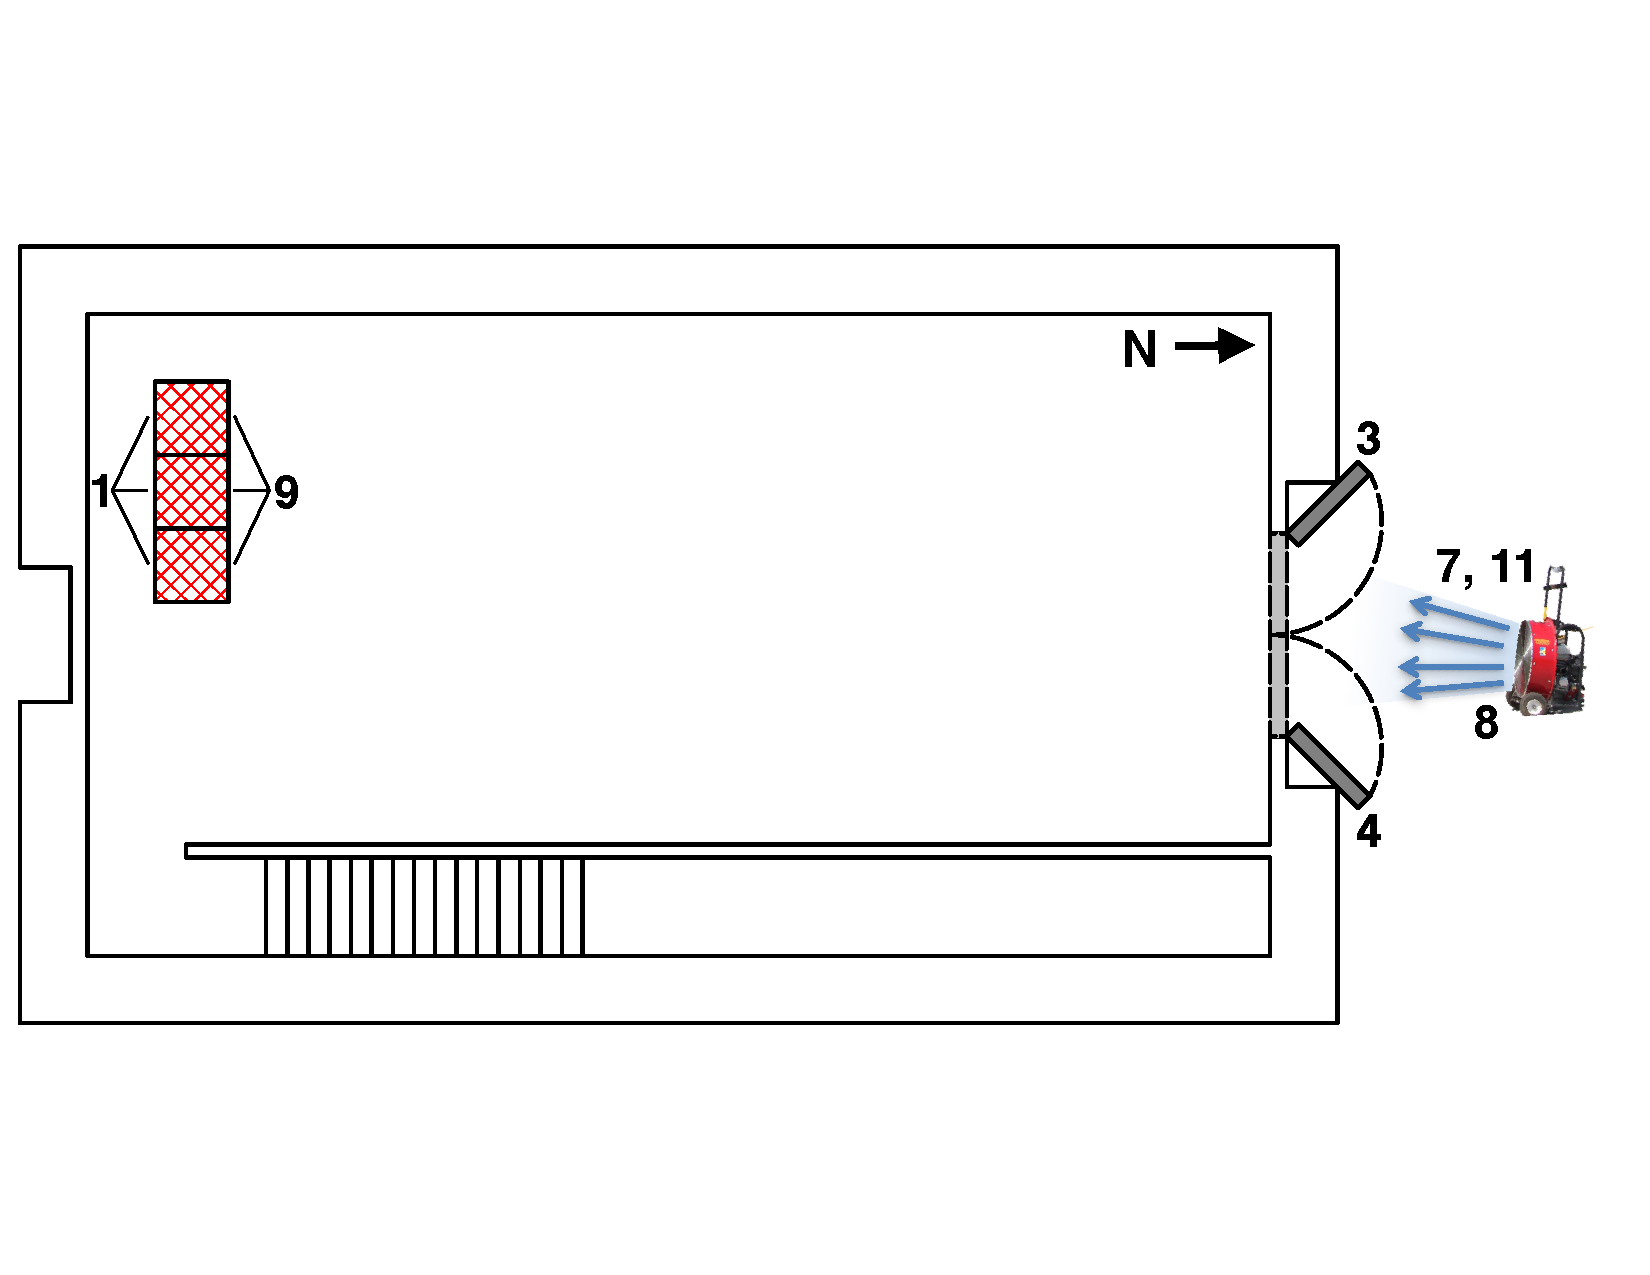
\includegraphics[width=0.95\columnwidth]{Figures/Floor_Plans/West_Structure_1st_Floor_Test_22}
% \end{minipage}
% \caption{Tests 22--23 layout and event times.}
% \label{fig:west_test_22}
% \end{figure}

\begin{figure}[!ht]
\renewcommand{\baselinestretch}{1}
\begin{minipage}[b]{0.88\columnwidth}
\begin{center}
	\begin{tabular}{lcc}
	\multicolumn{3}{c}{Event Times (sec) for Tests~22--23 Data Files} \\
	\toprule
	\multicolumn{1}{c}{\textbf{Event}} 			& \textbf{Test 22}	& \textbf{Test 23} \\
	\midrule
	~(1)~  All burners on 						&   0	  			&	 0			\\
	~(2)~  2nd floor west double door opened 	&   194		  		&    130		\\
	~(3)~  1st floor west double door opened 	&	314		  		&    252 	 	\\
	~(4)~  1st floor east double door opened 	&   450			  	&    371		\\
	~(5)~  2nd floor south exterior door closed &   511		  		&    N/A		\\
	~(6)~  2nd floor east double door opened	&   585			  	&    498		\\
	~(7)~  PPV fan on 							&   652			  	&    612		\\
	~(8)~  PPV fan off              			&   798			  	&    761		\\
	~(9)~  All burners off 						&   829			  	&    794		\\
	(10)   2nd floor south exterior door opened &   899			  	&    849		\\
	(11)   PPV fan on 	 						&   1065		  	&    940		\\
	(12)   2nd floor south exterior door closed &   1176		  	&    N/A		\\
	\bottomrule
	\end{tabular}
	% \begin{tabular}{|l|c|c|}
	% \multicolumn{3}{c}{Event Times (sec) for Tests~22--23 Data Files}
	% \vspace{5pt} \\
	% \hline
	% \multicolumn{1}{|c|}{Event}		    		& Test 22		  	& Test 23		\\
	% \hline \hline
	% ~(1)~  All burners on 						&   0	  			&	 0			\\
	% ~(2)~  2nd floor west double door opened 	&   194		  		&    130		\\
	% ~(3)~  1st floor west double door opened 	&	314		  		&    252 	 	\\
	% ~(4)~  1st floor east double door opened 	&   450			  	&    371		\\
	% ~(5)~  2nd floor south exterior door closed &   511		  		&    N/A		\\
	% ~(6)~  2nd floor east double door opened	&   585			  	&    498		\\
	% ~(7)~  PPV fan on 							&   652			  	&    612		\\
	% ~(8)~  PPV fan off              			&   798			  	&    761		\\
	% ~(9)~  All burners off 						&   829			  	&    794		\\
	% (10)   2nd floor south exterior door opened &   899			  	&    849		\\
	% (11)   PPV fan on 	 						&   1065		  	&    940		\\
	% (12)   2nd floor south exterior door closed &   1176		  	&    N/A		\\
	% \hline
	% \end{tabular}
\end{center}
\end{minipage}
\begin{minipage}[b]{\columnwidth}
	\vspace{15pt}
	\centering
	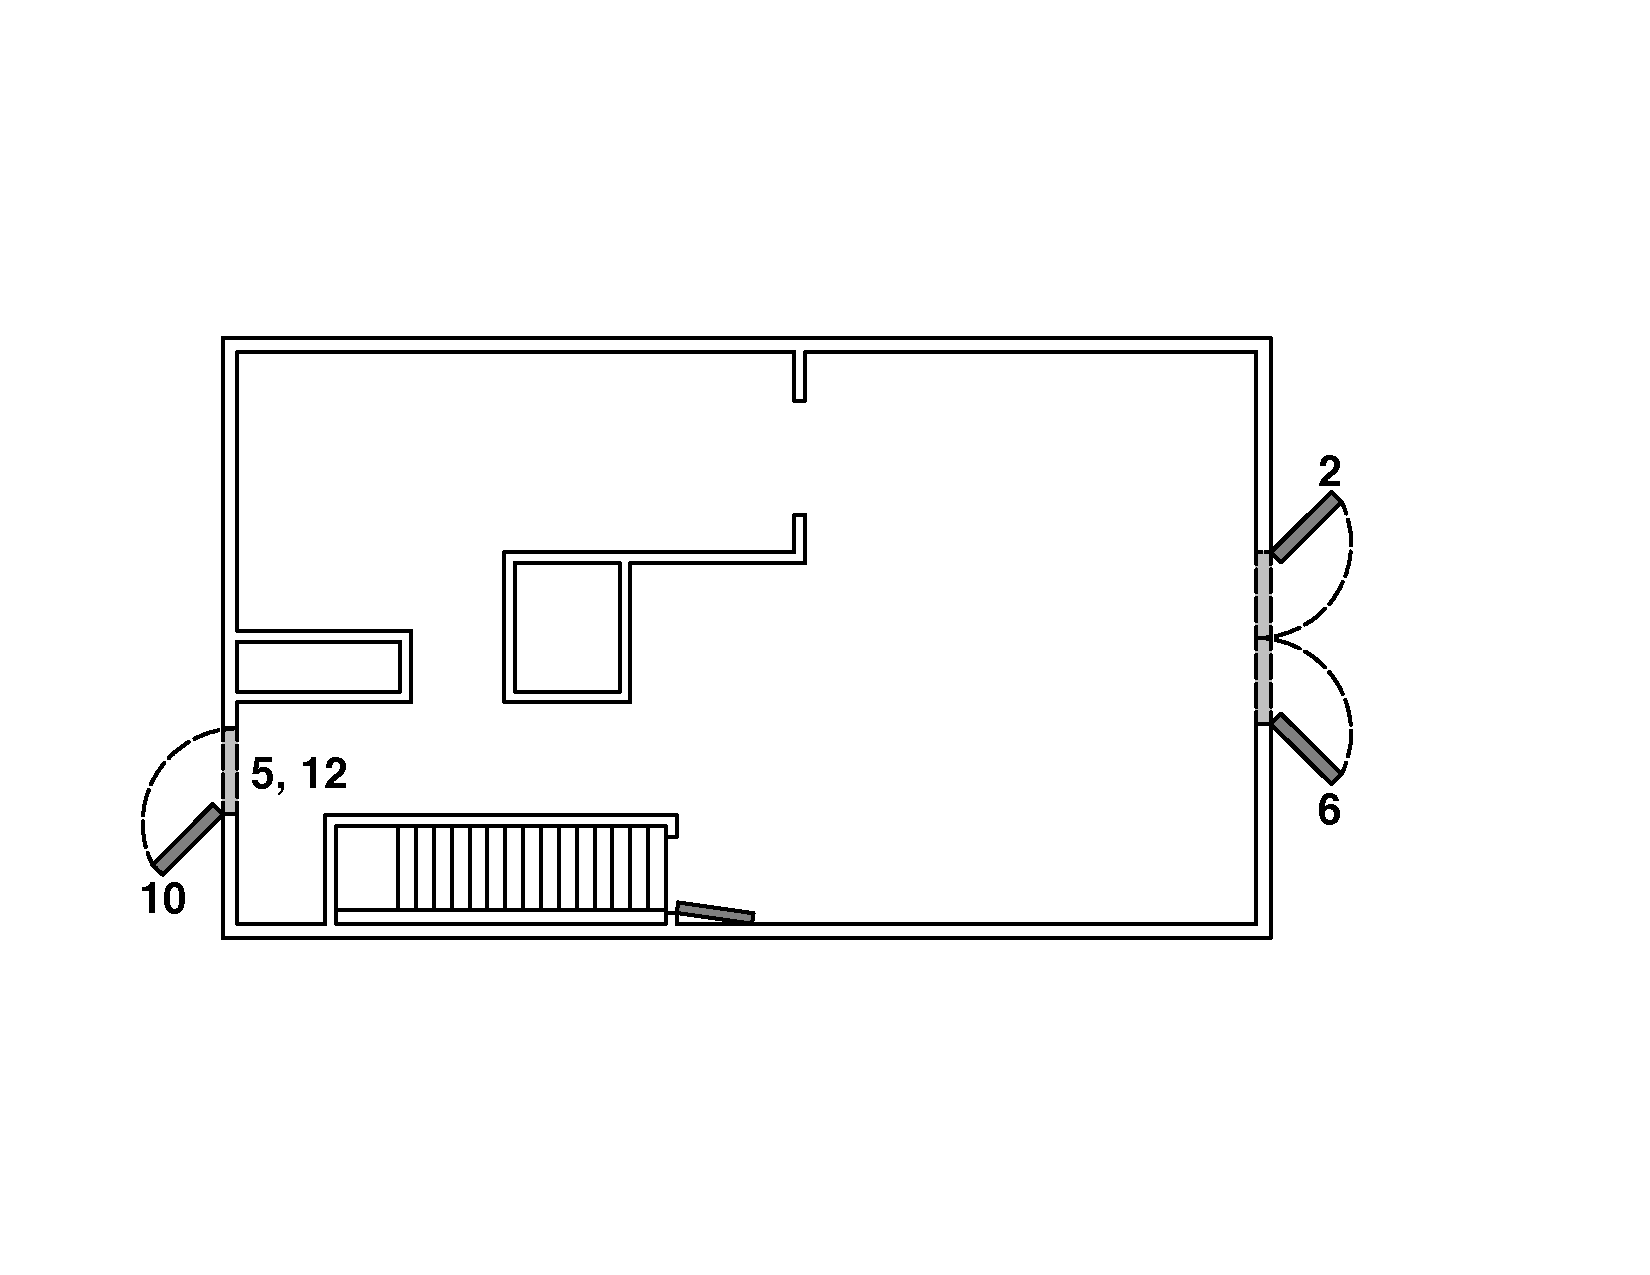
\includegraphics[width=\columnwidth]{Figures/Floor_Plans/West_Structure_2nd_Floor_Test_22}
	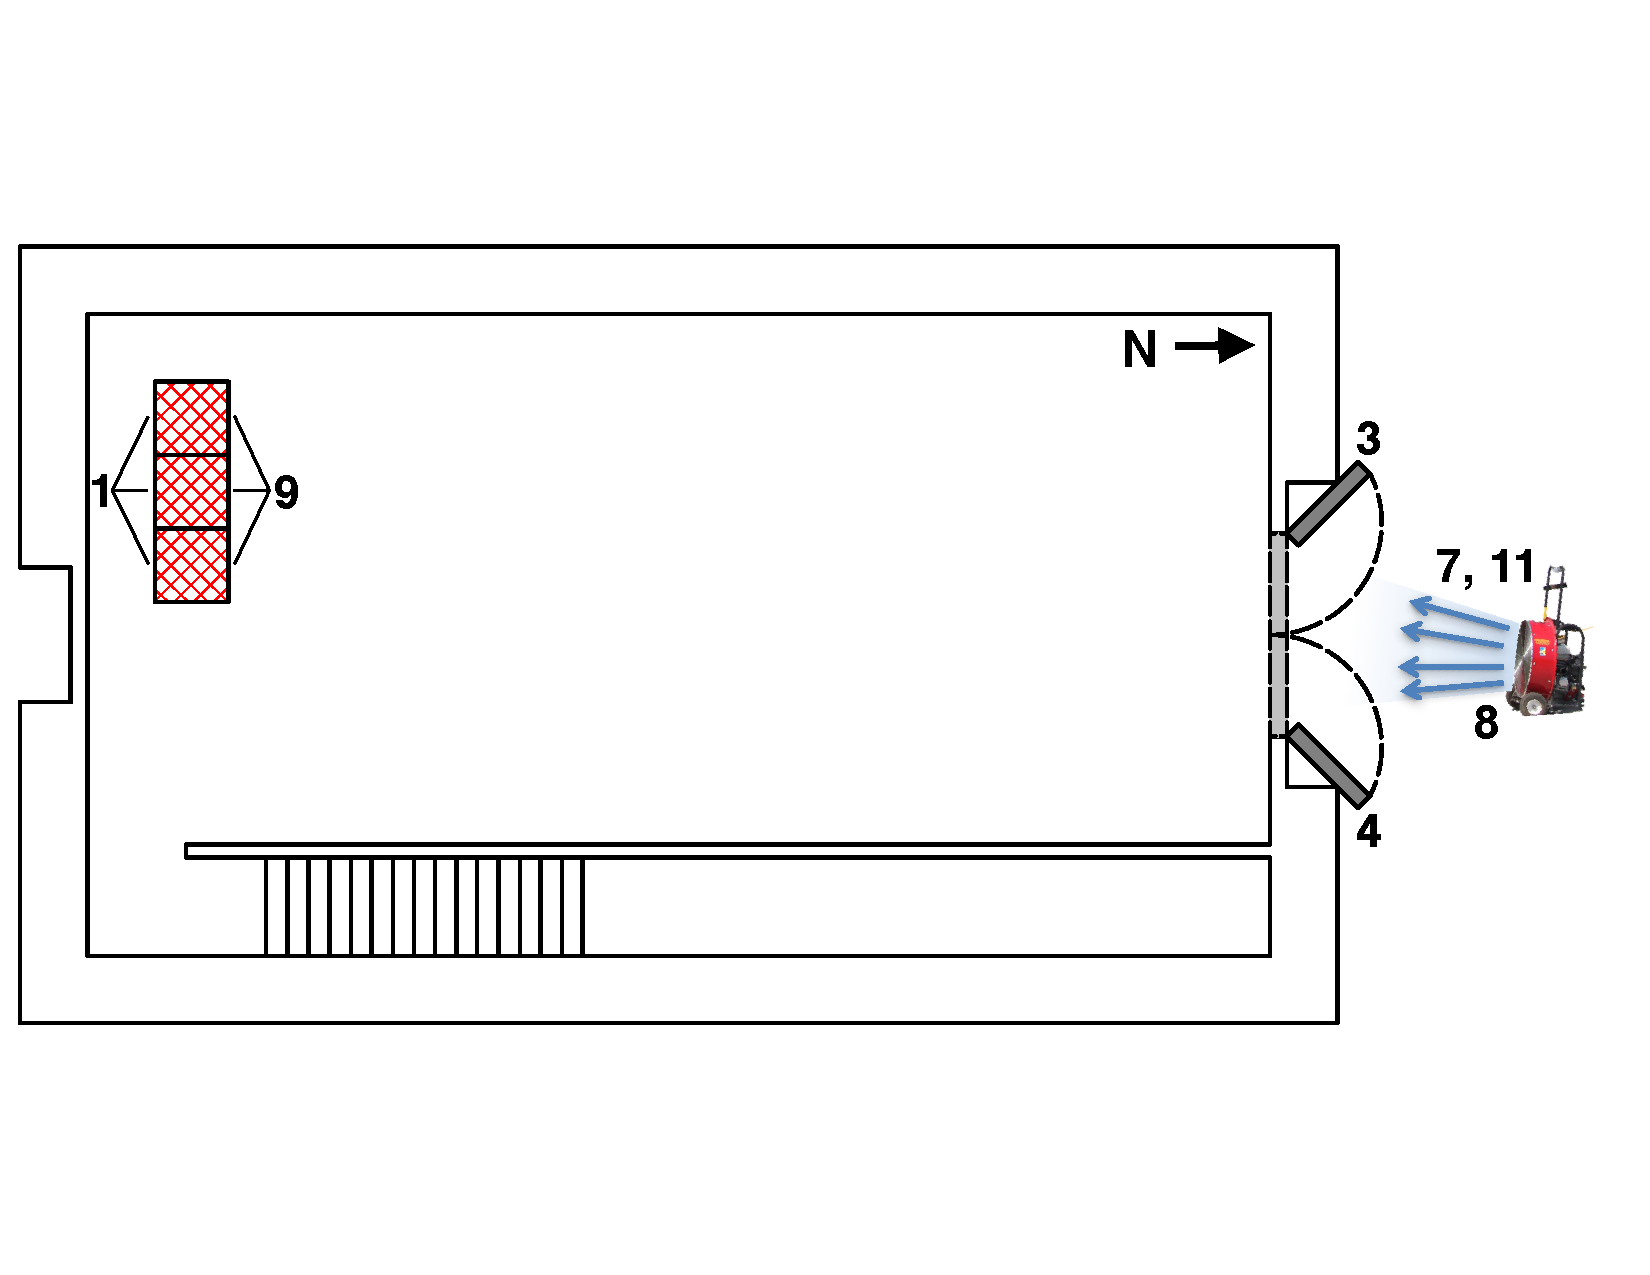
\includegraphics[width=0.95\columnwidth]{Figures/Floor_Plans/West_Structure_1st_Floor_Test_22}
\end{minipage}
\renewcommand{\baselinestretch}{1}
\caption{Tests 22--23 layout and event times.}
\label{fig:west_test_22}
\end{figure}
\FloatBarrier

\subsection{Tests~24 \& 25}

As with Tests~22 and 23, Tests~24 and 25 followed a nearly identical procedure. The starting configuration for Test~24 had the south exterior door on the second level in the opened position, while the starting configuration for Test~25 had the same door in the closed position. During both tests, the stairwell door was unable to completely close. When it was in the ``closed'' position at the beginning of each test, there was a 152~mm (6.0~in) gap between the door and its frame. Figure~\ref{fig:west_test_24} includes a floor plan schematic and table of event times corresponding to the data files for Tests~24 and 25. A 0.61~m (2.0~ft) diameter PPV fan located 2.3~m (7.5~ft) away from the first level double doors and aimed at the center of the west double door was used towards the end of both tests.

% \begin{figure}[!ht]
% \begin{minipage}[b]{0.8\columnwidth}
% 	\begin{flushleft}
% 	\begin{tabular}{lcc}
% 	\multicolumn{3}{c}{Event Times (s) for Tests 24--25 Data Files} \\
% 	\toprule
% 	\multicolumn{1}{c}{\textbf{Event}} 			& \textbf{Test 24}	& \textbf{Test 25} \\
% 	\midrule
% 	~(1)~ All burners on 						&   0		  		&	 0			\\
% 	~(2)~ Interior stairwell door opened 		&   144		  		&    112		\\
% 	~(3)~ 1st floor west double door opened 	&	265		  		&    244 	 	\\
% 	~(4)~ 2nd floor west double door opened 	&   383			  	&    353		\\
% 	~(5)~ 2nd floor south exterior door closed	&   452			  	&    N/A		\\
% 	~(6)~ 2nd floor south exterior door opened	&   502			  	&    474		\\
% 	~(7)~ PPV fan on 							&   624			  	&    594 		\\
% 	~(8)~ All burners off 						&   746 		  	&    721		\\
% 	~(9)~ 2nd floor east double door opened 	&   877			  	&    N/A		\\
% 	(10)  1st floor east double door opened		& 	N/A 			& 	 836		\\
% 	\bottomrule
% 	\end{tabular}
% 	\end{flushleft}
% \end{minipage}
% \begin{minipage}[b]{0.9\columnwidth}
% 	\vspace{15pt}
% 	\centering
% 	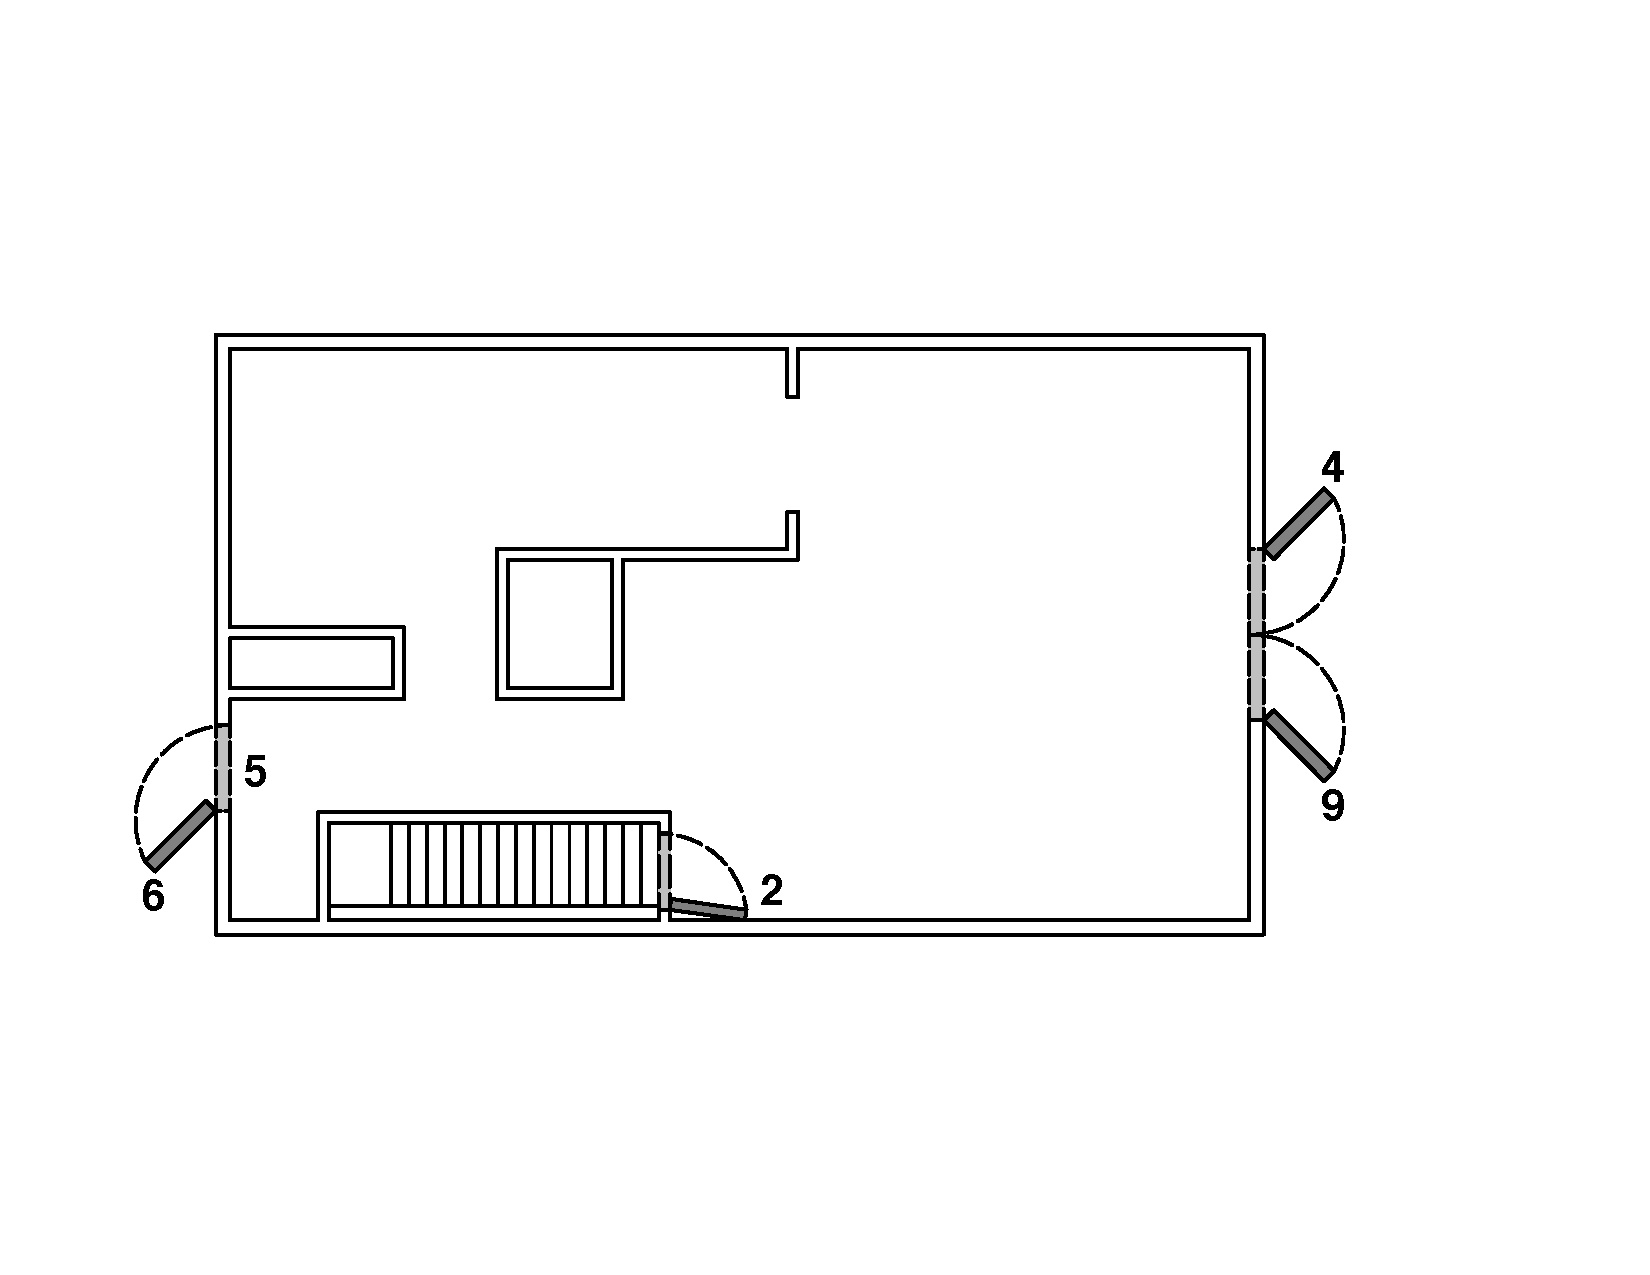
\includegraphics[width=\columnwidth]{Figures/Floor_Plans/West_Structure_2nd_Floor_Test_24}
% 	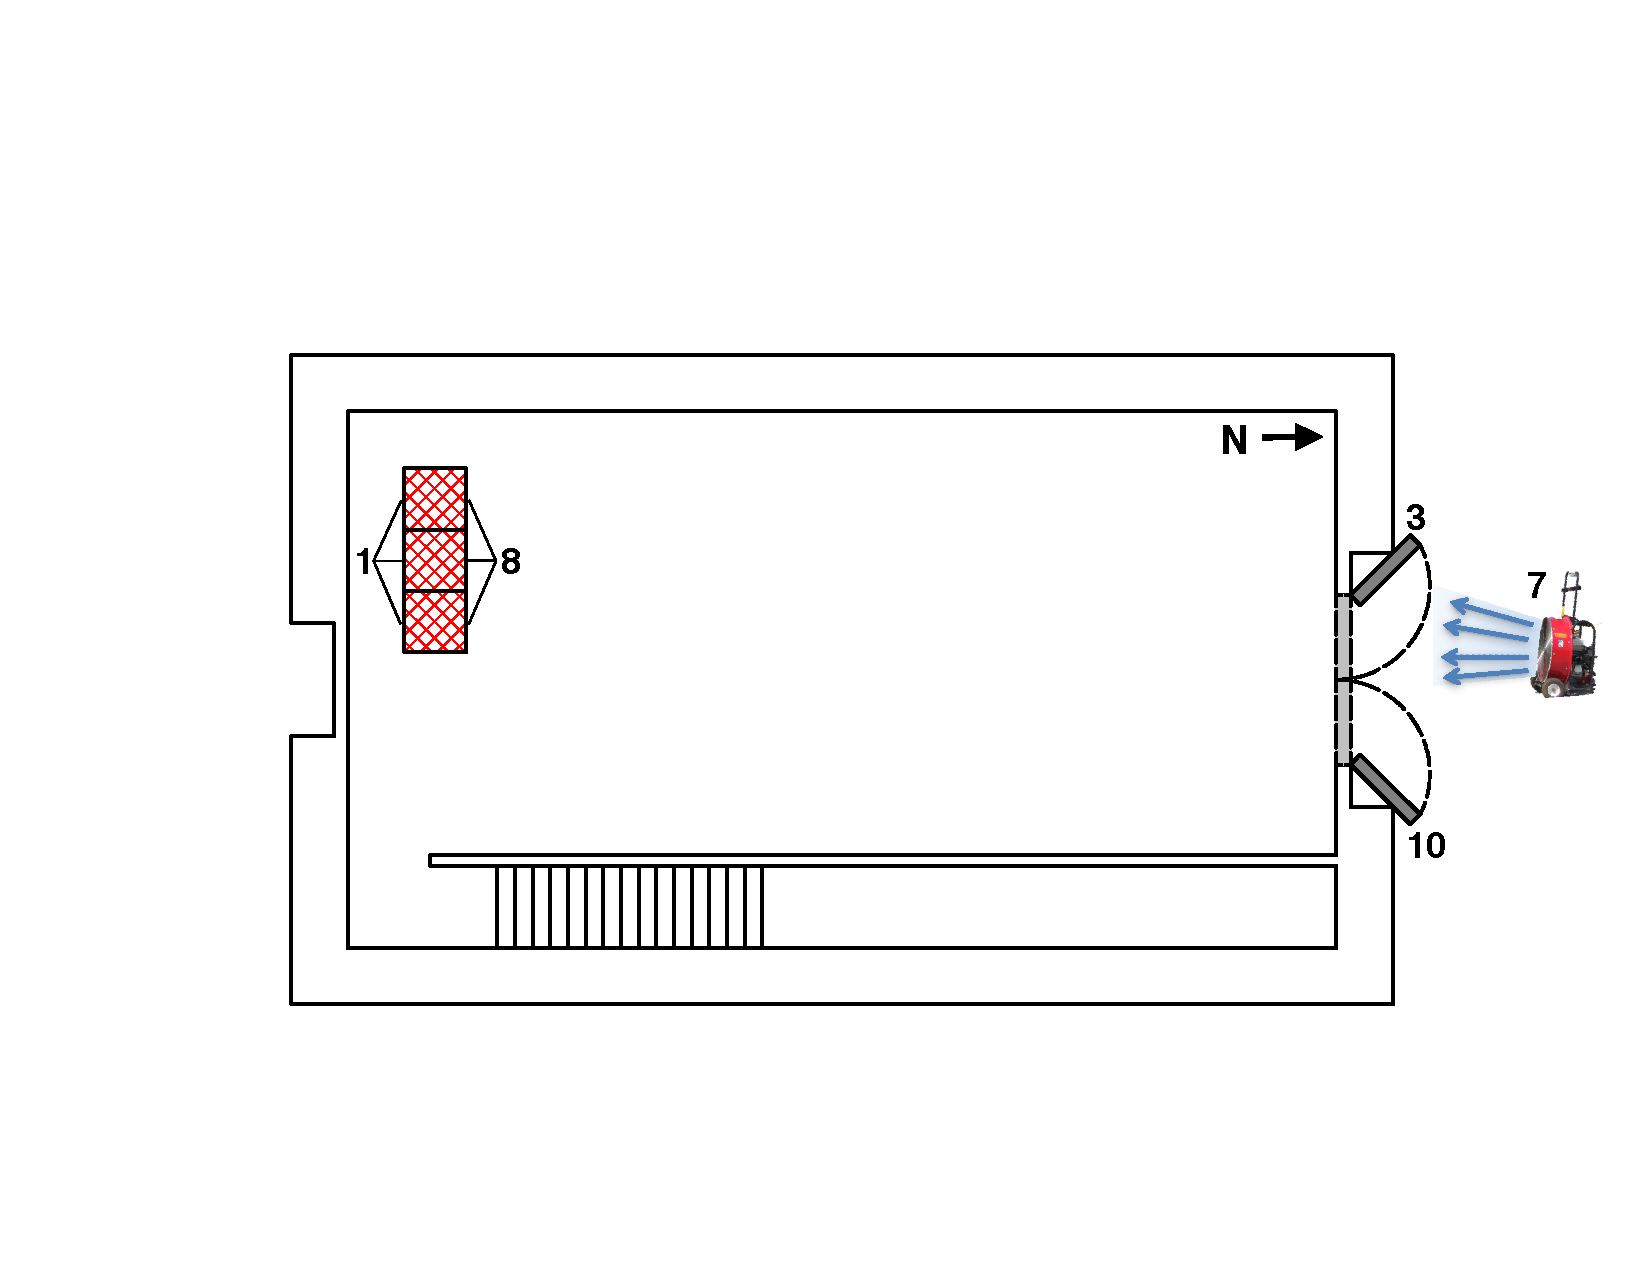
\includegraphics[width=0.95\columnwidth]{Figures/Floor_Plans/West_Structure_1st_Floor_Test_24}
% \end{minipage}
% \caption{Tests 24--25 layout and event times.}
% \label{fig:west_test_24}
% \end{figure}
% \clearpage

\begin{figure}[!ht]
\renewcommand{\baselinestretch}{1}
\begin{minipage}[b]{0.88\columnwidth}
\begin{center}
	% \begin{tabular}{|l|c|c|}
	% \multicolumn{3}{c}{Event Times (sec) for Tests~24--25 Data Files}
	% \vspace{5pt} \\
	% \hline
	% \multicolumn{1}{|c|}{Event}		    		& Test 24		  	& Test 25		\\
	% \hline \hline
	% ~(1)~ All burners on 						&   0		  		&	 0			\\
	% ~(2)~ Interior stairwell door opened 		&   144		  		&    112		\\
	% ~(3)~ 1st floor west double door opened 	&	265		  		&    244 	 	\\
	% ~(4)~ 2nd floor west double door opened 	&   383			  	&    353		\\
	% ~(5)~ 2nd floor south exterior door closed	&   452			  	&    N/A		\\
	% ~(6)~ 2nd floor south exterior door opened	&   502			  	&    474		\\
	% ~(7)~ PPV fan on 							&   624			  	&    594 		\\
	% ~(8)~ All burners off 						&   746 		  	&    721		\\
	% ~(9)~ 2nd floor east double door opened 	&   877			  	&    N/A		\\
	% (10)  1st floor east double door opened		& 	N/A 			& 	 836		\\
	% \hline
	% \end{tabular}
	\begin{tabular}{lcc}
	\multicolumn{3}{c}{Event Times (sec) for Tests 24--25 Data Files} \\
	\toprule
	\multicolumn{1}{c}{\textbf{Event}} 			& \textbf{Test 24}	& \textbf{Test 25} \\
	\midrule
	~(1)~ All burners on 						&   0		  		&	 0			\\
	~(2)~ Interior stairwell door opened 		&   144		  		&    112		\\
	~(3)~ 1st floor west double door opened 	&	265		  		&    244 	 	\\
	~(4)~ 2nd floor west double door opened 	&   383			  	&    353		\\
	~(5)~ 2nd floor south exterior door closed	&   452			  	&    N/A		\\
	~(6)~ 2nd floor south exterior door opened	&   502			  	&    474		\\
	~(7)~ PPV fan on 							&   624			  	&    594 		\\
	~(8)~ All burners off 						&   746 		  	&    721		\\
	~(9)~ 2nd floor east double door opened 	&   877			  	&    N/A		\\
	(10)  1st floor east double door opened		& 	N/A 			& 	 836		\\
	\bottomrule
	\end{tabular}
\end{center}
\end{minipage}
\begin{minipage}[b]{\columnwidth}
	\vspace{15pt}
	\centering
	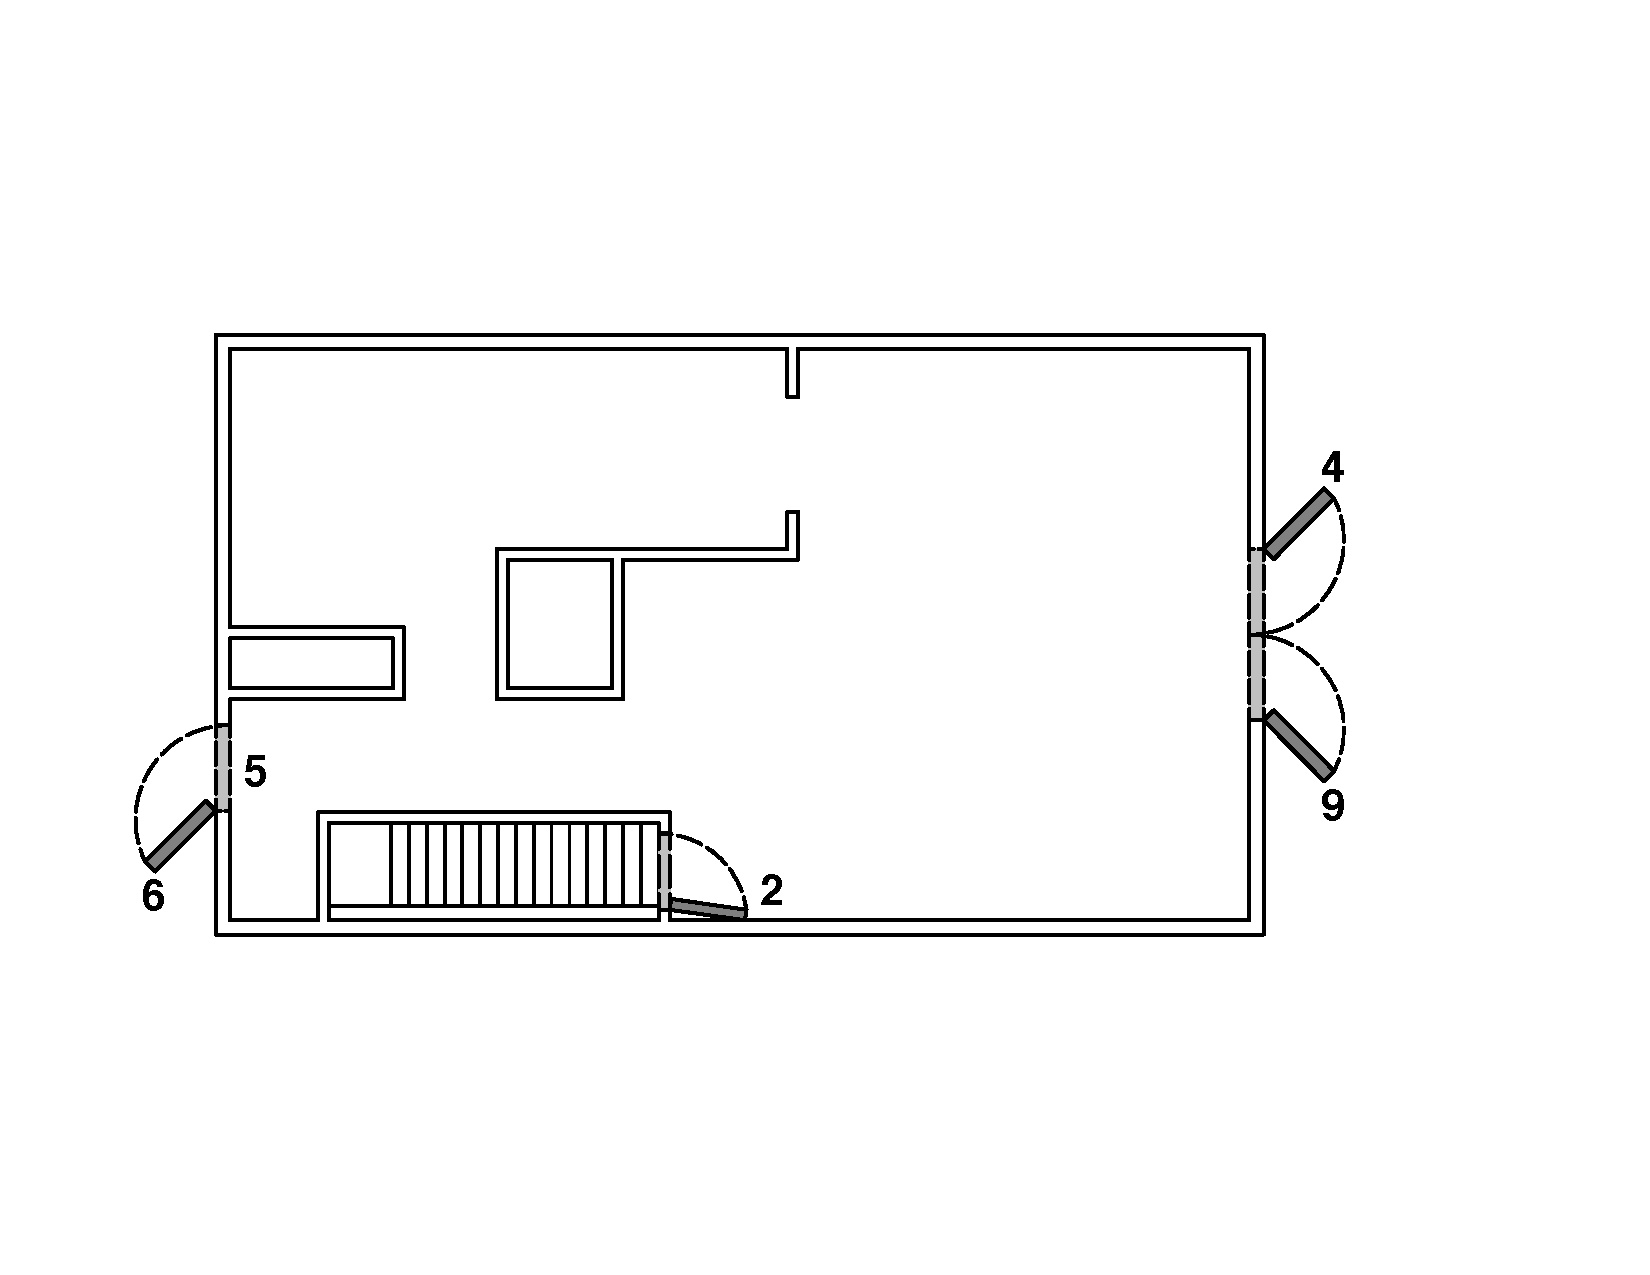
\includegraphics[width=\columnwidth]{Figures/Floor_Plans/West_Structure_2nd_Floor_Test_24}
	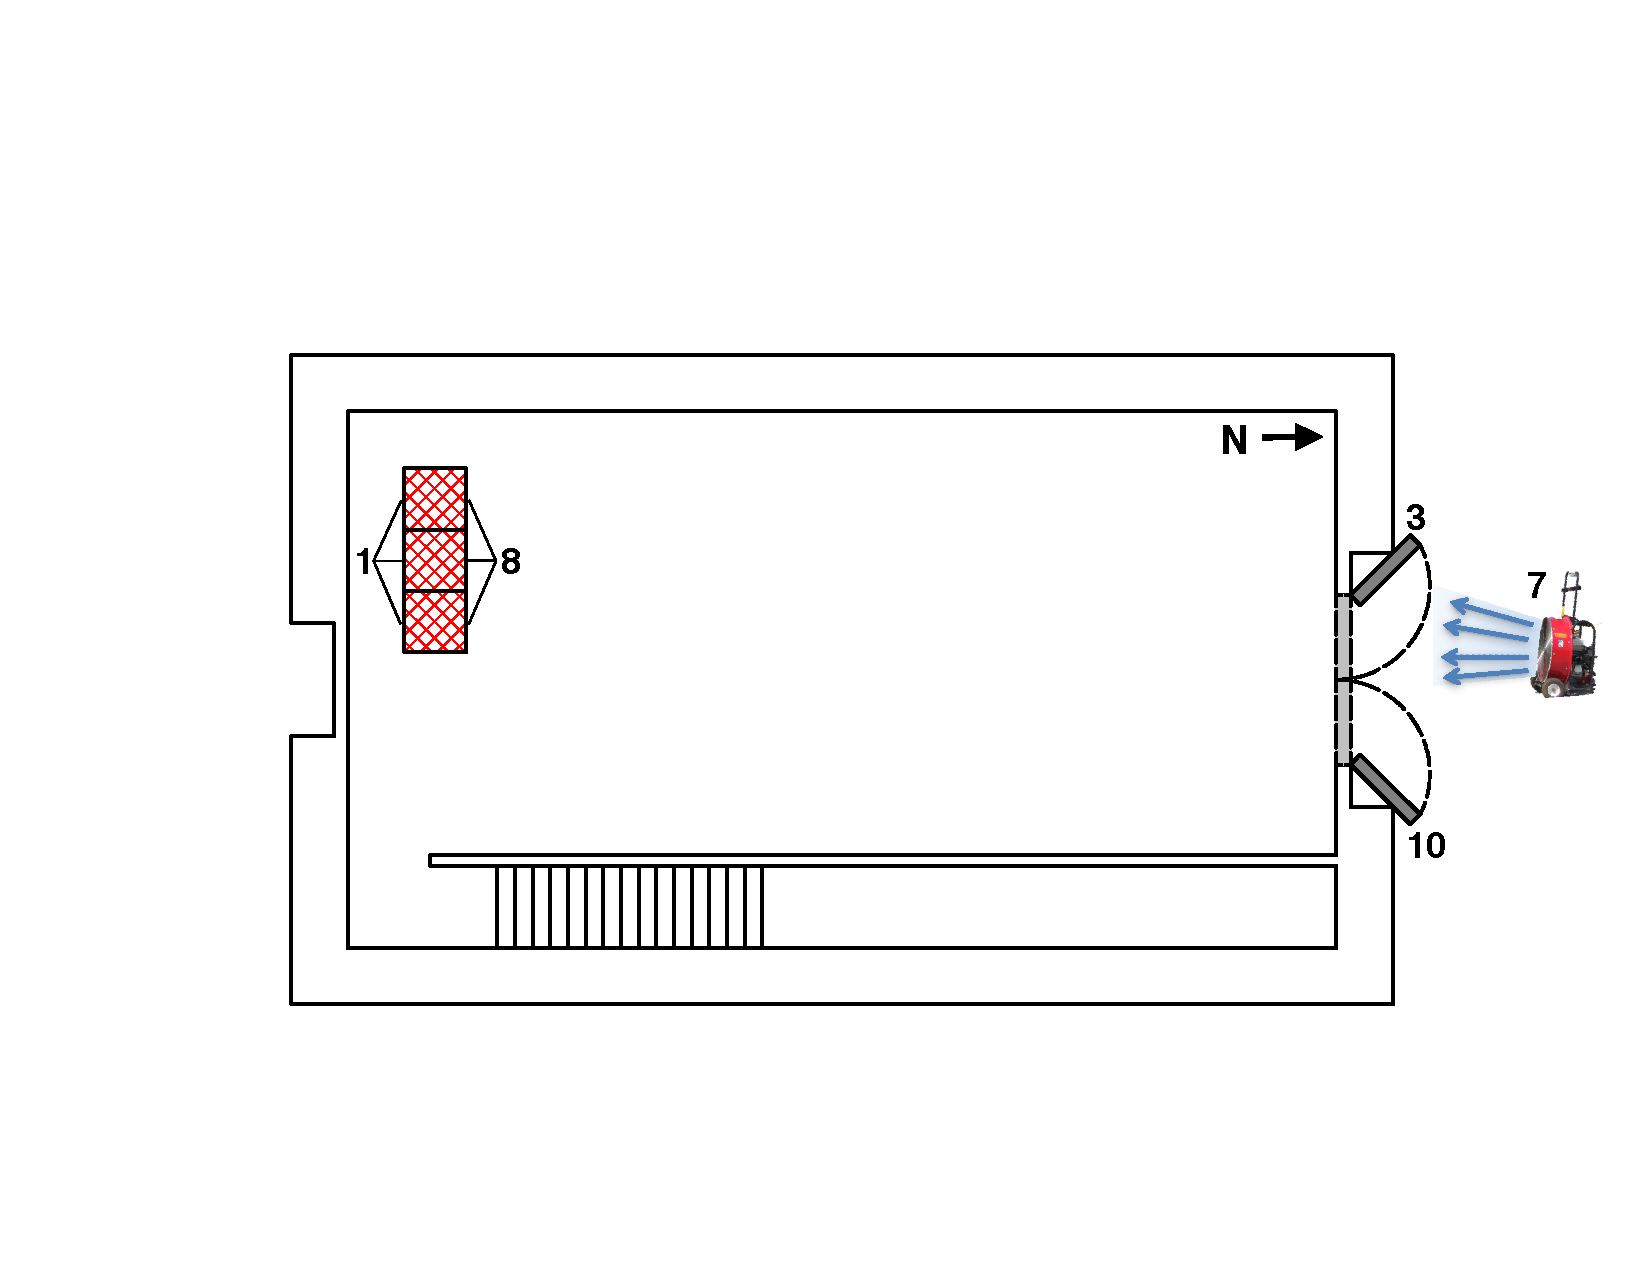
\includegraphics[width=0.95\columnwidth]{Figures/Floor_Plans/West_Structure_1st_Floor_Test_24}
\end{minipage}
\renewcommand{\baselinestretch}{1}
\caption{Tests 24--25 layout and event times.}
\label{fig:west_test_24}
\end{figure}
\renewcommand{\baselinestretch}{2}
\FloatBarrier

%%%%%%%%%%%%%%%%%%%%%%%%%%%%%%%%
% CHAPTER 4: Model Description %
%%%%%%%%%%%%%%%%%%%%%%%%%%%%%%%%
%................................
% Notes about things to add/edit 
%................................
% >> Think about using MQH with known HRR and comparing accuracy
% >> Read through FDS guides to search for anything to add to chapter intro
% >> Generate smokeview models and save for fig? 
% >> Add Refs to Material table
% >> Justification for TMPFRONT = 500?
% >> MQH Input values
% >> DESCRIBE PREDEFINED PROPERTIES of Propane and CO2
% >> ELABORATE gas phase combustion/N2 background species SEE [pg 180 of user guide]
%%%%%%%%%%%%%%%%%%%%%%%%%%%%%%%%%%%%%%%%%%%%%%%%%%%%%%%%%%%%%%%%%%%%%

\renewcommand{\thechapter}{4}
\label{chap:model_descr}

\chapter{Numerical Model Description}
% Brief summary of FDS
Fire Dynamics Simulator (version 6.5.3)~\cite{FDS_Users_Guide}, a CFD model of thermally-driven fluid flow that is developed and maintained by NIST, was used to model the burner experiments described in Chapter~\ref{chap:exp_procedure}. FDS numerically solves a form of the Navier-Stokes equations for low-speed ($Ma < 0.3$), fire-driven flows with an emphasis on smoke and heat transport from fires. The FDS Technical Reference Guide~\cite{FDS_Tech_Guide} provides a complete description of the model, including the formulation of the equations and numerical algorithm utilized by the software. FDS is mathematically verified~\cite{FDS_Verification_Guide} and validated against a continually growing database of experimental data from different fire scenarios~\cite{FDS_Validation_Guide}. 

% Computational domain description
FDS performs calculations within a computational domain that is composed of rectilinear volumes called meshes. Each mesh is divided into three-dimensional rectangular computational cells. Using the laws of mass, momentum, and energy conservation, FDS calculates the gas density, velocity, temperature, pressure, and species concentration within each grid cell and determines the generation and movement of fire gases within the domain. In general, the number of cells within each mesh (i.e., the grid cell size) determines the resolution of the mesh: the smaller the size of the cells, the higher the resolution of the simulation. However, increasing the resolution of a simulation increases the need for more computational resources and produces a longer simulation run time. Thus, it's critical to determine a proper grid cell size for the meshes within an FDS computational domain based on available resources and desired level of model fidelity. In order to select an appropriate cell size for the simulations of the gas burner experiments, a mesh sensitivity analysis, described in Section~\ref{subsec:mesh}, was performed.  

% List of other prescribed inputs
In addition to defining the meshes and cells within the computational domain, other types of input data must be known and considered to properly formulate a fire model. Key input parameters that were specified within the FDS input files and additional characteristics of the model setup are described throughout the sections of this chapter.

\section{Computational Domain}
The computational domain for the East Structure simulations was set to span 14~m in the $x$ direction, 8~m in the $y$ direction, and 3~m in the $z$ direction, and the computational domain for the West Structure simulations spanned 14~m in the $x$ direction, 8~m in the $y$ direction, and 5.4~m in the $z$ direction. Each structure was centered between the $x$ and $y$ boundaries of its respective domain, and the ground of the first floor was set at $z=0$~m. The structures were modeled based on the dimensions shown in the floor plan drawings presented in Figures~\ref{fig:east_dimensioned_plan} and \ref{fig:west_dimensioned_plan} of Chapter~\ref{chap:exp_setup}. 

The entire computational domain for each simulation was divided into eight different meshes to utilize the Message-Passing Interface (MPI) feature of FDS that allows multiple computers, or multiple cores on one computer, to run a multi-mesh FDS job with each mesh as its own process. All simulations were executed by utilizing MPI parallel processing on a multi-processor Linux machine.

\subsection{Numerical Mesh}
\label{subsec:mesh}
According to the FDS User Guide, a measure of how well the flow field is resolved for a simulation involving buoyant plumes is provided by the result of the expression $D^*/\delta x$, known as the resolution index (RI), in which $D^*$ is the characteristic fire diameter defined as
\begin{equation}
\label{eq:Dstar}
	D^* = \left( \frac{\dot{Q}}{\rho_\infty c_p T_\infty \sqrt{g}}\right)^{2/5}
\end{equation}
where $\dot{Q}$ is the total heat release rate of the fire (kW), $\delta x$ is the nominal size of each grid cell (m), $\rho_\infty$ is the density (kg/m$^3$) of the surrounding gas (air), $c_p$ is the specific heat (kJ/(kg$\cdot$K)) surrounding air, $T_\infty$ is the temperature (K) surrounding air, and $g$ is gravity (m/s$^2$). 

To determine the grid cell size to prescribe the meshes within the model simulations, a mesh sensitivity study was performed for the Test~4 simulation in the East Structure and the Test~25 simulation in the West Structure. Tests~4 and 25 were selected for the analysis because they have shorter durations compared to other East Structure and West Structure experiments. Three different grid cell sizes corresponding to the coarse, medium, and fine meshes were used in the mesh sensitivity study: 14~cm, 10~cm, and 5~cm for the East Structure and 7~cm for the West Structure, respectively. These corresponded to RI values ranging from 5--7 for the coarse grid, 8--11 for the medium grid, and 15--20 for the fine grid. Previous FDS validation work from the U.S. Nuclear Regulatory Commission suggests that RI values from 4 to 16 generated adequate results in terms of engineering calculations~\cite{NUREG_1824}.

The characteristic fire diameter (and thus, the RI values) were similar for all nine FDS simulations, so the results from the mesh sensitivity analysis of one simulation was used to determine and justify the grid cell size for all burner experiment simulations conducted within the same structure. From the analysis, it was determined that a cell size of 10~cm (medium mesh) was appropriate for all nine simulations. This cell size results in a domain with 336,000 computational grid cells for the East Structure and a domain with 604,800 computational grid cells for the West Structure. The results of the sensitivity study are presented and discussed in Section~\ref{sec:mesh_studies} of Chapter~\ref{chap:results_disc}.

As previously mentioned, the computational domain was divided into eight equally sized meshes. The first mesh was defined by the \verb|MESH| namelist group and was assigned a \verb|MULT_ID| quantity corresponding to a multiplier utility defined by the \verb|MULT| namelist group. For example, the mesh in the Test~2 input file was defined by the following
\begin{quote}
\begin{verbatim}
&MESH IJK=35,40,30, XB=-1.5,2.0,-0.8,3.2,0.0,3.0, 
     MULT_ID='mesh' / 
\end{verbatim}
\end{quote}
with the assigned \verb|MULT_ID| defined as 
\begin{quote}
\begin{verbatim}
&MULT ID='mesh', DX=3.5, DY=4.0, I_UPPER=3, J_UPPER=1 /
\end{verbatim}
\end{quote}
This creates an array of eight meshes with identical \verb|z1| and \verb|z2| bounds from \verb|0.0| to \verb|3.0| and \verb|x1, x2, y1, y2| bounds that vary according to the following:
\begin{equation*}
\begin{split}
	x1' &= -1.5+3.5i \textrm{~~for~} 0 \leq i \leq 3 \\
	x2' &= 2.0+3.5i \textrm{~~~~for~} 0 \leq i \leq 3 \\
	y1' &= -0.8+4j \textrm{~~for~} 0 \leq j \leq 1 \\
	y2' &= 3.2+4j \textrm{~~~~for~} 0 \leq j \leq 1 \\
\end{split}
\end{equation*}
where $i$ and $j$ are integers.

\section{Source Fire Characterization}
% Burner/fire definition details "held at a constant temperature of 500~$^\circ$C"
Each propane burner in the simulations was modeled as having steel sides and a 0.6~m~x~0.6~m surface located 0.1~m above the ground with a specified mass flux (kg/(m$^2$s)) of propane in the positive $z$ direction corresponding to the burner's heat release rate. In order to provide an example of the exact lines that were included in the input files to define the burners and propane fires in this manner, the following lines defined the surfaces with specified propane mass fluxes corresponding to the heat release rate of each burner in the Test~2 FDS input file: 
\begin{quote}
\begin{verbatim}
&SURF ID='BURNER 1', MASS_FLUX(1)=0.0264, SPEC_ID(1)='PROPANE', 
    COLOR='RED', RAMP_MF(1)='burner1', TMP_FRONT=500. /
&SURF ID='BURNER 2', MASS_FLUX(1)=0.0246, SPEC_ID(1)='PROPANE', 
    COLOR='RED', RAMP_MF(1)='burner2', TMP_FRONT=500. /
&SURF ID='BURNER 3', MASS_FLUX(1)=0.0060, SPEC_ID(1)='PROPANE', 
    COLOR='RED', RAMP_MF(1)='burner3', TMP_FRONT=500. /
\end{verbatim}
\end{quote}

Additionally, the following lines were used in the Test~2 input file to define each gas burner as having steel sides and a top surface with the specified propane mass flux from above:
\begin{quote}
\begin{verbatim}
&OBST XB= 0.60, 1.20, 4.90, 5.50, 0.00, 0.10, 
    SURF_IDS='BURNER 1','STEEL PLATE','STEEL PLATE' /
&OBST XB= 0.60, 1.20, 4.30, 4.90, 0.00, 0.10, 
    SURF_IDS='BURNER 2','STEEL PLATE','STEEL PLATE' /
&OBST XB= 0.60, 1.20, 3.70, 4.30, 0.00, 0.10, 
    SURF_IDS='BURNER 3','STEEL PLATE','STEEL PLATE' /
&OBST XB= 0.60, 0.60, 3.70, 5.50, 0.10, 0.20, 
    SURF_ID='STEEL PLATE' /
&OBST XB= 1.20, 1.20, 3.70, 5.50, 0.10, 0.20, 
    SURF_ID='STEEL PLATE' /
&OBST XB= 0.60, 1.20, 3.70, 3.70, 0.10, 0.20, 
    SURF_ID='STEEL PLATE' /
&OBST XB= 0.60, 1.20, 5.50, 5.50, 0.10, 0.20, 
    SURF_ID='STEEL PLATE' /
\end{verbatim}
\end{quote}

The heat release rates listed in Table~\ref{table:exp_summary} from Chapter~\ref{chap:exp_procedure} were used to determine the values of propane mass flux to prescribe to the burners defined in the FDS input files for Tests~5--6 and Tests~22--25. The propane mass flux, $\dot{m}_{C_3H_8}''$, was calculated using the equation
\begin{equation}
  \dot{m}_{C_3H_8}''=\frac{\dot{Q}}{A\Delta h_c}
\end{equation}
% density_C3H8 = 1.82   # [kg/m^3]; at 300 K 
% delH_C3H8 = 46334.6   # [kJ/kg]
%                 Mass flux [kg/m^2-s]
% Test      Burner 1          Burner 2          Burner 3
% 2         0.0264            0.0246            0.006
% 3         0.0312            0.0252            0.0102
% 4         0.0330            0.0252            0.0096
% in which $\dot{Q}$ is the burner heat release rate; $A$ is the area of the top surface of the burner, 0.36~m$^2$ for all burners; and $\Delta h_c$ is the effective heat of combustion of the fuel (propane), which was taken to be 46334.6~kJ/kg [REF?].
in which $\dot{Q}$ is the burner heat release rate, $A$ is the area of the top surface of the burner, and $\Delta h_c$ is the effective heat of combustion of the fuel (propane).

As mentioned in Chapter~\ref{chap:exp_procedure}, the rate of propane flow to the burners was not able to be accurately measured during Tests~2--4. Instead, the heat release rates prescribed to the simulations of Tests~2--4 during the periods in which one, two, and three burners were ignited were estimated using the hot gas layer (HGL) temperature of the fire room during each period in conjunction with the following correlation derived by McCaffrey, Quintiere, and Harkleroad (MQH correlation) for compartment fires~\cite{McCaffery:1}: 
\begin{equation}
\label{eq:MQH}
\begin{split}
  T_g &= 6.85 \left( \frac{\dot{Q}^2}{A_0 \sqrt{H_0} h_k A_T}\right)^{1/3}+T_{\infty} \\
  &\Rightarrow~\dot{Q} = \left[A_0  \sqrt{H_0} h_k A_T \left( \frac{T_g-T_{\infty}}{6.85}\right)^3\right]^{1/2}
\end{split}
\end{equation}
where $\dot{Q}$ is the heat release rate of the fire (kW), $A_0$ is the area of the compartment opening (m$^2$), $H_0$ is the height of the compartment opening (m), $h_k$ is the effective heat transfer coefficient (kW/(m$^2$K)), $A_T$ is the total area of the compartment enclosing surfaces (m$^2$), $T_g$ is the temperature of the upper gas layer (K), and $T_{\infty}$ is the ambient temperature (K). The HGL temperatures of the fire room were calculated using the experimental data from the thermocouple arrays in the fire room (A1 and A2). The exact methodology of obtaining the hot gas layer temperature from the thermocouple data is outlined in Chapter~\ref{chap:results_disc}. 

% calculated as $\sqrt{k\rho c/t}$ $A_0$ as the area of the open doorway in the fire room, 1.8~m$^2$; $H_0$ as the doorway height, 2.0~m; 
Using Equation~\ref{eq:MQH}, the heat release rates for the periods with one, two, and three burners ignited were estimated and used to determine the propane mass flux value of each burner surface in the FDS input files for Tests~2--4. Table~\ref{table:test_over} lists the heat release rates obtained from this method, rounded to the nearest 10~kW.

\begin{table}[!ht]
% \renewcommand{\baselinestretch}{1}
\caption[Tests~2--4 Estimated Heat Release Rates Using MQH Correlation.]{Tests~2--4 Heat Release Rates (kW) Estimated using the Average Hot Gas Layer Temperature and MQH Correlation.}
\begin{center}
\begin{tabular}{cccc}
\toprule
\textbf{Test~\#} & \textbf{1 Burner Ignited} & \textbf{2 Burners Ignited} & \textbf{3 Burners Ignited}  \\
\midrule
2 & 440 & 850 & 950 \\
3 & 520 & 940 & 1110 \\
4 & 550 & 970 & 1130 \\
\hline
\end{tabular}
\end{center}
\label{table:test_over}
\end{table}
% \renewcommand{\baselinestretch}{2}
% Details about combustion reactions
The reaction mechanisms for combustion in all simulations were modeled using the default mixing-controlled, simple chemistry model (reaction rate is infinite and limited only by species concentrations) and were specified via the following code:
\begin{quote}
\begin{verbatim}
&REAC ID = 'R1'
      FUEL = 'PROPANE'
      SPEC_ID_NU='PROPANE','OXYGEN','CARBON MONOXIDE',
        'WATER VAPOR','SOOT'
      NU= -1,-3.456,2.912,4.0,0.088 
\end{verbatim}
\end{quote}
\noindent which corresponds to the following single-step reaction mechanism for propane:
\begin{center}
\ce{C3H8 + 3.456O2 -> 2.912CO + 4H2O + 0.088C}
\end{center}
Additionally, the production of carbon dioxide was tracked via
\begin{quote}
\begin{verbatim}
&REAC ID = 'R2'
      FUEL = 'CARBON MONOXIDE'
      SPEC_ID_NU='CARBON MONOXIDE','OXYGEN','CARBON DIOXIDE'
      NU= -1,-0.5,1
      RADIATIVE_FRACTION=0.30   
\end{verbatim}
\end{quote}
and nitrogen was set as the background species. Note, FDS has built-in properties for a number of different fuels, including \verb|PROPANE| and \verb|CARBON MONOXIDE|. Therefore, it was not necessary to explicitly list thermophysical properties for the prescribed fuels. Finally, because of the presence of multiple chemical reactions, gas phase combustion was eliminated by setting \verb|SUPPRESSION=.FALSE.| on the \verb|MISC| line.

\FloatBarrier
\section{Additional Input Parameters}
In addition to those already presented in the previous sections, a variety of other parameters were specified within the simulation input files. These include the ambient temperature, timing information, thermophysical properties of materials that weren't already predefined by FDS, leakage associated with the structure, and the different devices to model the various types of instrumentation used during the physical experiments.

% Ambient T
The ambient temperature was explicitly set in each input file based on the average temperature throughout the test structure before ignition, which was obtained by averaging the temperatures measured by the thermocouple arrays throughout the structure at the start of the test. The average ambient temperatures ranged from 35~$^\circ$C to 62~$^\circ$C. The variation in ambient temperatures is a result of the fact that some of the burner tests were conducted shortly after another fire experiment in the same structure, so significant residual heat from the first test was present within the structure at the start of the next test.

% Timing information
The timing information specified within the FDS input files consisted of the simulation run time and event times listed in the tables presented with Figures~\ref{fig:Tests_2-4_layout}--\ref{fig:west_test_24} in Chapter~\ref{chap:exp_procedure}. The vents were modeled by first defining a hole via the \verb|HOLE| namelist group at the location of the vent, setting an obstruction via the \verb|OBST| namelist group to cover the hole at the start of the simulation, and assigning a control to the obstruction using the \verb|CTRL| namelist group. The control was set to a timer defined by the \verb|DEVC| namelist group and used a ramp function defined by the \verb|RAMP| namelist group to change the \verb|PERMIT_HOLE| value for the obstruction from \verb|.FALSE.| to \verb|.TRUE.| at the time of the vent opening. For example, the following lines were included within the Test~2 FDS input file to initially define the north side, east double door as closed and then opened at 538~s:
\begin{quote}
\begin{verbatim}
&HOLE XB=10.99,11.11, 2.10, 3.00, 0.00, 2.00 
     / Cut-out for North-East Door
&OBST XB=11.00,11.10, 2.10, 3.00, 0.00, 2.00, SURF_ID='DOOR', 
     PERMIT_HOLE=.FALSE., CTRL_ID='east controller' 
     / North-East Door
&CTRL ID='east controller', FUNCTION_TYPE='CUSTOM', 
     INPUT_ID='east timer', RAMP_ID='east cycle' /
&DEVC ID='east timer', QUANTITY='TIME', XYZ=0,0,0 /
&RAMP ID='east cycle', T=   0., F= 1 /
&RAMP ID='east cycle', T= 537., F= 1 /
&RAMP ID='east cycle', T= 538., F=-1 /
\end{verbatim}
\end{quote}

% Defined Materials
Four materials were explicitly defined via the \verb|MATL| namelist group to assign to different surfaces within the simulation input files. The specific heat, thermal conductivity, and density of each material was defined by assigning appropriate values to the \verb|SPECIFIC_HEAT| (kJ/(kg$\cdot$K)), \verb|CONDUCTIVITY| (W/(m$\cdot$K)), and \verb|DENSITY| (kg/m$^3$) parameters within the corresponding \verb|MATL| namelist group. For example, concrete was defined by the lines
\begin{quote}
\begin{verbatim}
 &MATL ID            = 'CONCRETE'                                              
        CONDUCTIVITY  = 1.75        
        SPECIFIC_HEAT = 1.04       
        DENSITY       = 2200. /
\end{verbatim}
\end{quote}
A complete list of the explicitly defined materials and their properties are listed in Table~\ref{table:material_props}.
\begin{table}[!ht]
\cprotect\caption{Various Materials Defined Within Each FDS Input File and the Corresponding \verb|MATL| Namelist Group Parameter Values.}
\begin{center}
\begin{tabular}{ccccc}
\toprule
\textbf{Material}  &  \multirow{2}{*}{\textbf{Reference}} & \verb|SPECIFIC_HEAT|	        &  \verb|CONDUCTIVITY| 	      & \verb|DENSITY| 	\\
\verb|ID|		       &                                      &   \textbf{(kJ/(kg$\cdot$K))} 	& 	\textbf{(W/(m$\cdot$K))} 	&  \textbf{(kg/m$^3$)} 		\\
\midrule
Steel 			       & 	     \cite{Gross:Props}             &	        0.48   		            &  		 62.0	 		              & 	 7850  			\\
Gypsum 			       & 	     \cite{Gross:Props}             &	        0.90                  &  		 0.16	 		              & 	  770  			\\
Concrete 		       & 	     \cite{Gross:Props}             &	        1.04   		            &  		 1.75	 		              & 	 2200  			\\
Fiber Cement 	     &       \cite{Durock:specs}            &		      1.0     		          &  		 0.15	 		              & 	 1300  			\\
\bottomrule
\end{tabular}
\end{center}
\label{table:material_props}
\end{table}
\FloatBarrier
The materials in Table~\ref{table:material_props} were explicitly specified within the FDS input files to ensure that the solid boundary surfaces throughout the model were properly defined as described in Chapter~\ref{chap:exp_setup}. For example, based on the description of the exterior walls from Chapter~\ref{chap:exp_setup}:  
\begin{quote}
``The first floor of each structure had outer walls composed of interlocking concrete blocks measuring 0.6~m (2.0~ft) wide\ldots Two layers of 16~mm (0.63~in) Type X gypsum board lined the steel studs, and a layer of 13~mm (0.5~in) thick Durock cement board covered the gypsum board.''
\end{quote}
the surface of the exterior walls were defined in the FDS input file by the following lines:
\begin{quote}
\begin{verbatim}
&SURF ID            = 'EXTERIOR WALL'
      DEFAULT       = .TRUE.
      RGB           = 150,150,150
      MATL_ID       = 'FIBER CEMENT','GYPSUM','CONCRETE'
      THICKNESS     = 0.013,0.03,0.610 /
\end{verbatim}
\end{quote}

% Leakage
To account for the structure leakage described in Chapter~\ref{chap:exp_setup}, the pressure zone leakage approach outlined by the FDS User Guide~\cite{FDS_Users_Guide} in which a leakage flow is computed via the program's HVAC model to capture bulk leakage through structure walls was used. This approach involves defining a pressure zone using the \verb|ZONE| namelist group and assigning a leakage area via the \verb|LEAK_AREA| quantity of the zone.

% Instrumentation and other devices
Various instrumentation devices can be modeled within FDS through the \verb|DEVC| namelist group. Different devices were specified in the FDS input files at the sensor locations described in Chapter~\ref{chap:exp_setup}. The \verb|QUANTITY| parameter within the \verb|DEVC| namelist group was set based on the type of sensor being modeled. Table~\ref{table:FDS_sensor_info} lists each type of sensor that was modeled, its corresponding \verb|QUANTITY| parameter, and the combined uncertainty associated with the \verb|QUANTITY| parameter as given by the FDS Validation Guide.  

\begin{table}[!ht]
\cprotect\caption{Instrumentation Specified within FDS Input File and Corresponding \verb|DEVC| Namelist Group Properties.}
\begin{center}
\begin{tabular}{ccc}
\toprule
\textbf{Instrumentation} & \textbf{Assigned}           & \textbf{Combined}       \\
\textbf{Type}                     & \verb|QUANTITY|             & \textbf{Uncertainty}        \\
\midrule
Thermocouple            & \verb|'THERMOCOUPLE'|       &     7~\%     \\
Gas Concentration       & \verb|'VOLUME FRACTION'|    &     8~\%     \\
BDP                     & \verb|'VELOCITY'|           &     8~\%     \\
Heat Flux Gauge         & \verb|'GAUGE HEAT FLUX'|    &     11~\%     \\
% Radiometer              & \verb|'RADIOMETER'|         &     11~\%     \\
\bottomrule
\end{tabular}
\end{center}
\label{table:FDS_sensor_info}
\end{table}
\FloatBarrier
% Finally, to model the PPV fan that was used after the burners were extinguished in Tests~2--4 and during Tests~22--25, an obstruction was created at the fan location and a surface was assigned to the front of the fan with a specified velocity normal to the side of the structure that was controlled by a timer and ramp, similar to the vent openings.  


%%%%%%%%%%%%%%%%%%%%%%%%%%%%%%%%%%%
% CHAPTER 5: Results + Discussion %
%%%%%%%%%%%%%%%%%%%%%%%%%%%%%%%%%%%
%................................
% Notes about things to add/edit 
%................................
% >> Add plots of gas data stochiometric stuff+
% >> Evaluate comparison of HF and Velocity data and decide if it should be included
% >> Average velocity along entire door?{}
% >> Flame height via video footage?
% >> Linear plots of parameters vs. each other
%%%%%%%%%%%%%%%%%%%%%%%%%%%%%%%%%%%%%%%%%%%%%%%%%%%%%%%%%%%%%%%%%%%%%
\renewcommand{\thechapter}{5}

\chapter{Results and Discussion}
\label{chap:results_disc}
Three different types of figures are presented in this chapter to assist with the discussion of the results. One type is presented with the discussion of the mesh sensitivity study results that were used to select an appropriate grid cell size for the simulations. The other two types are presented throughout the comparison of the predicted data output by the FDS simulations to the corresponding experimental data. 

\section{Mesh Sensitivity Studies}
\label{sec:mesh_studies}
Figures~\ref{fig:east_O2_sensitivity}--\ref{fig:west_cjet_sensitivity} show the oxygen volume fractions and ceiling jet temperatures output by FDS simulations of Test~4 and Test~25 using the coarse, medium, and fine grid sizes across the computational domain.
\begin{figure}[!h]
	\centering
	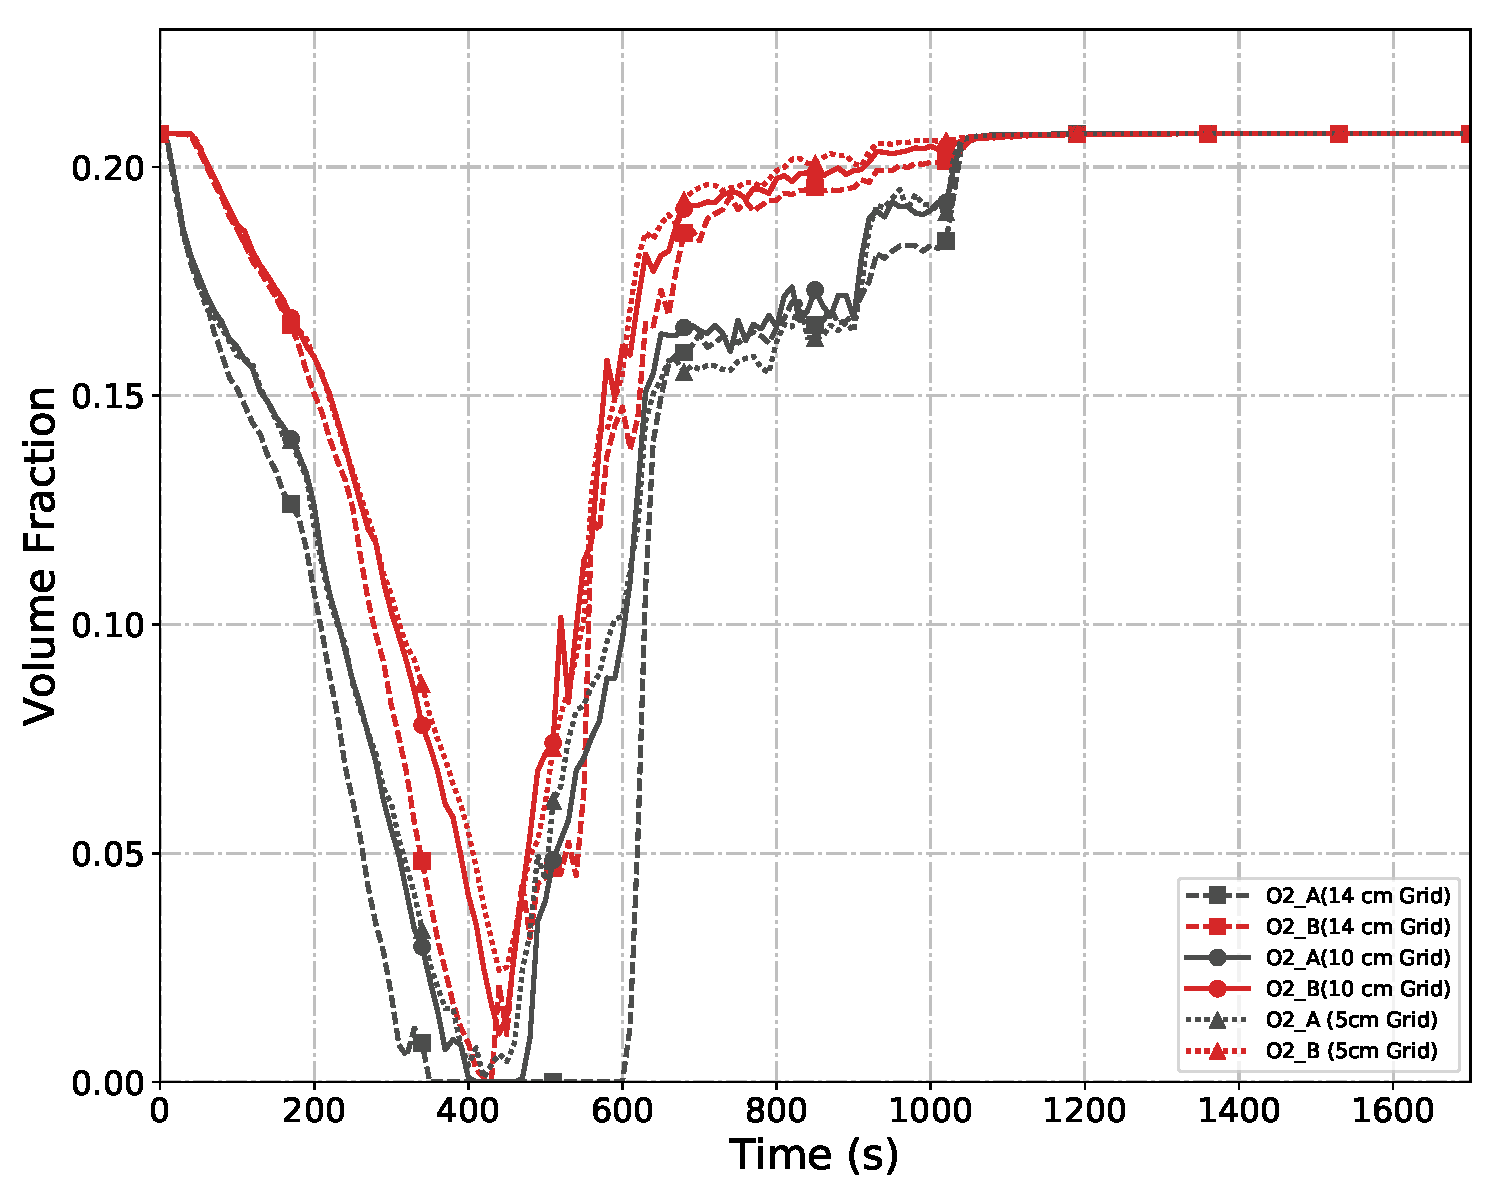
\includegraphics[width=\columnwidth]{Figures/Plots/Grid_Sensitivity/Gas_Concentration/Test_04_O2}
	\caption[$O_2$ concentrations for East Structure simulation with different grid cell sizes.]{$O_2$ concentrations output by the FDS simulation of Test~4 in the East Structure using three different grid cell sizes.}
	\label{fig:east_O2_sensitivity}
\end{figure}

\begin{figure}[!h]
	\centering
	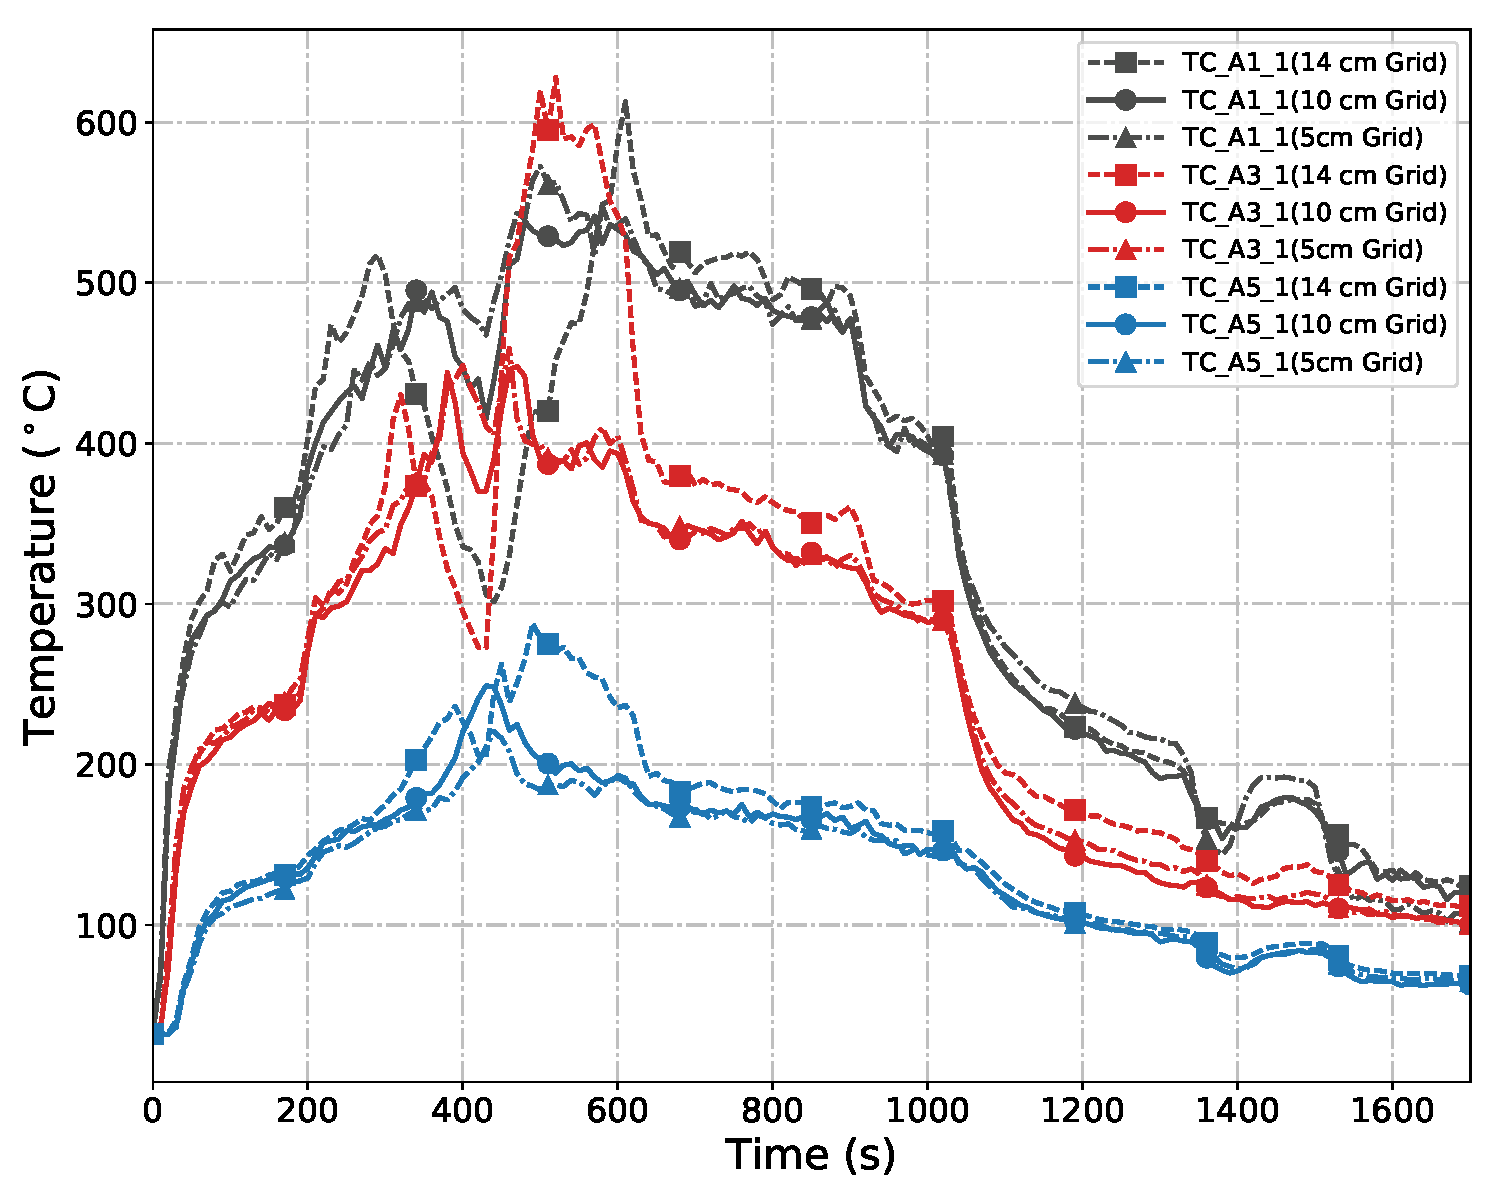
\includegraphics[width=0.87\columnwidth]{Figures/Plots/Grid_Sensitivity/Temperature/Test_04_cjet_1}
	\\~\\
	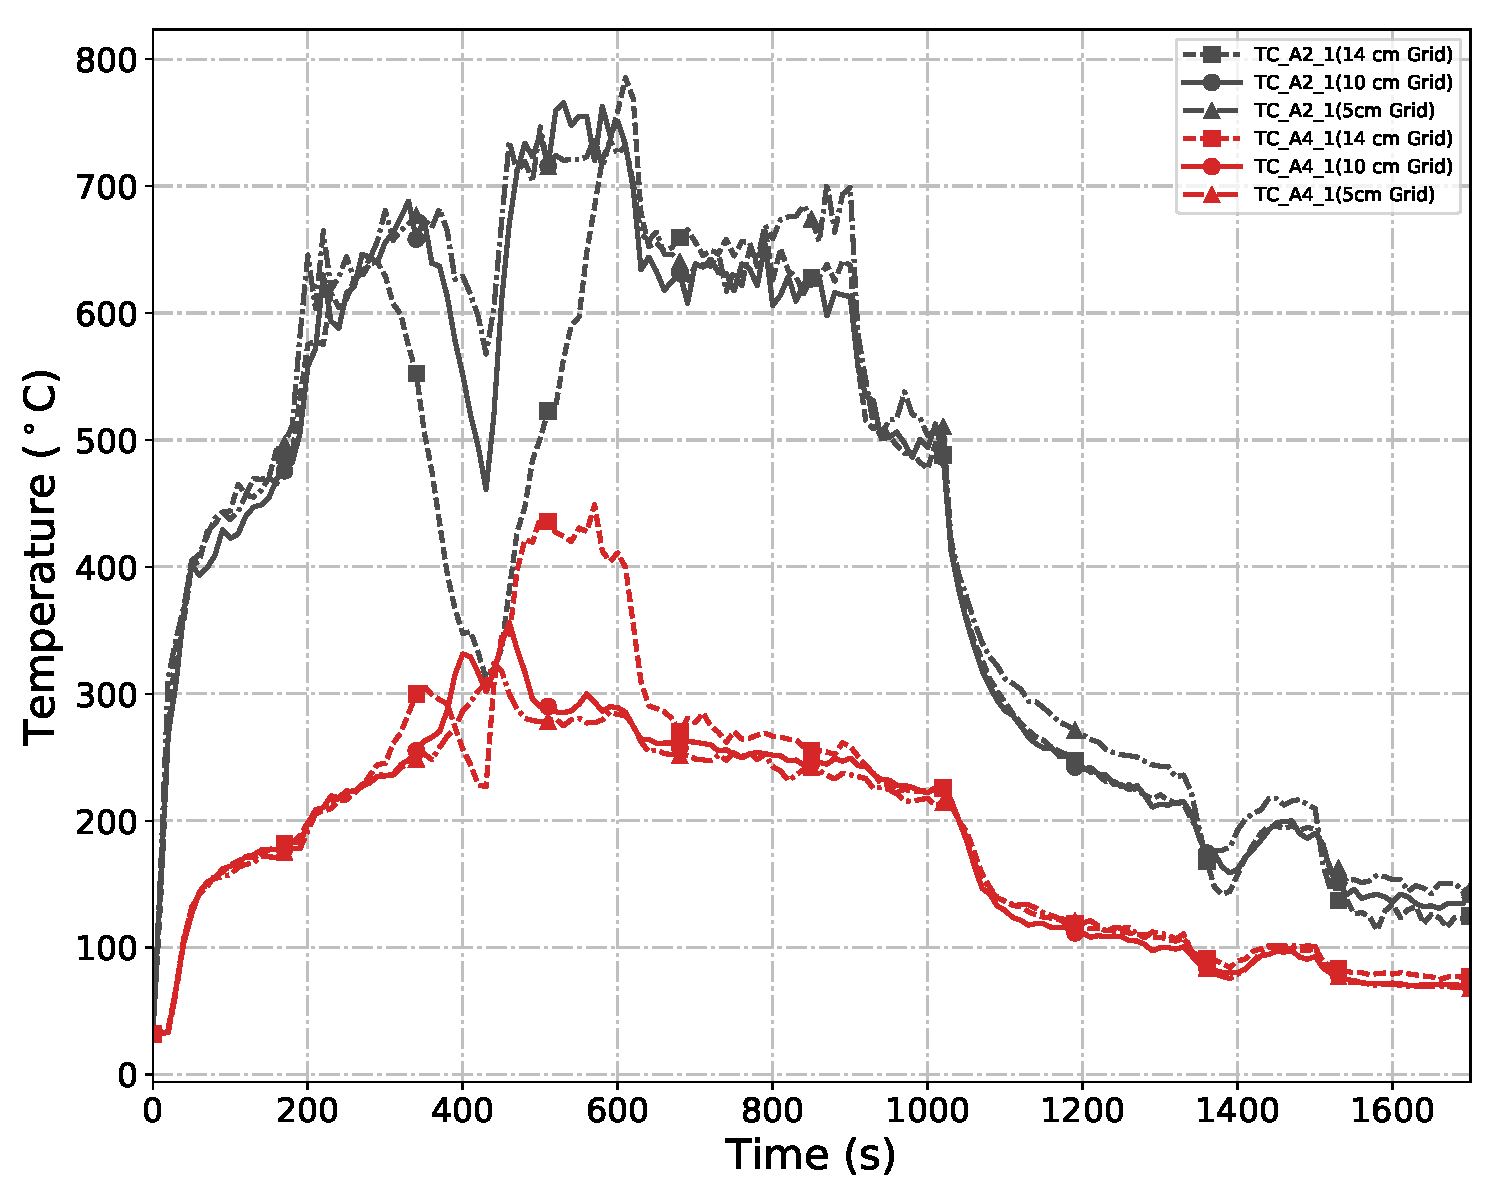
\includegraphics[width=0.87\columnwidth]{Figures/Plots/Grid_Sensitivity/Temperature/Test_04_cjet_2}
	\caption[Ceiling jet temperatures for East Structure simulation with different grid cell sizes.]{Ceiling jet temperatures output by the FDS simulation of Test~4 in the East Structure using three different grid cell sizes.}
	\label{fig:east_cjet_sensitivity}
\end{figure}

\begin{figure}[!h]
	\centering
	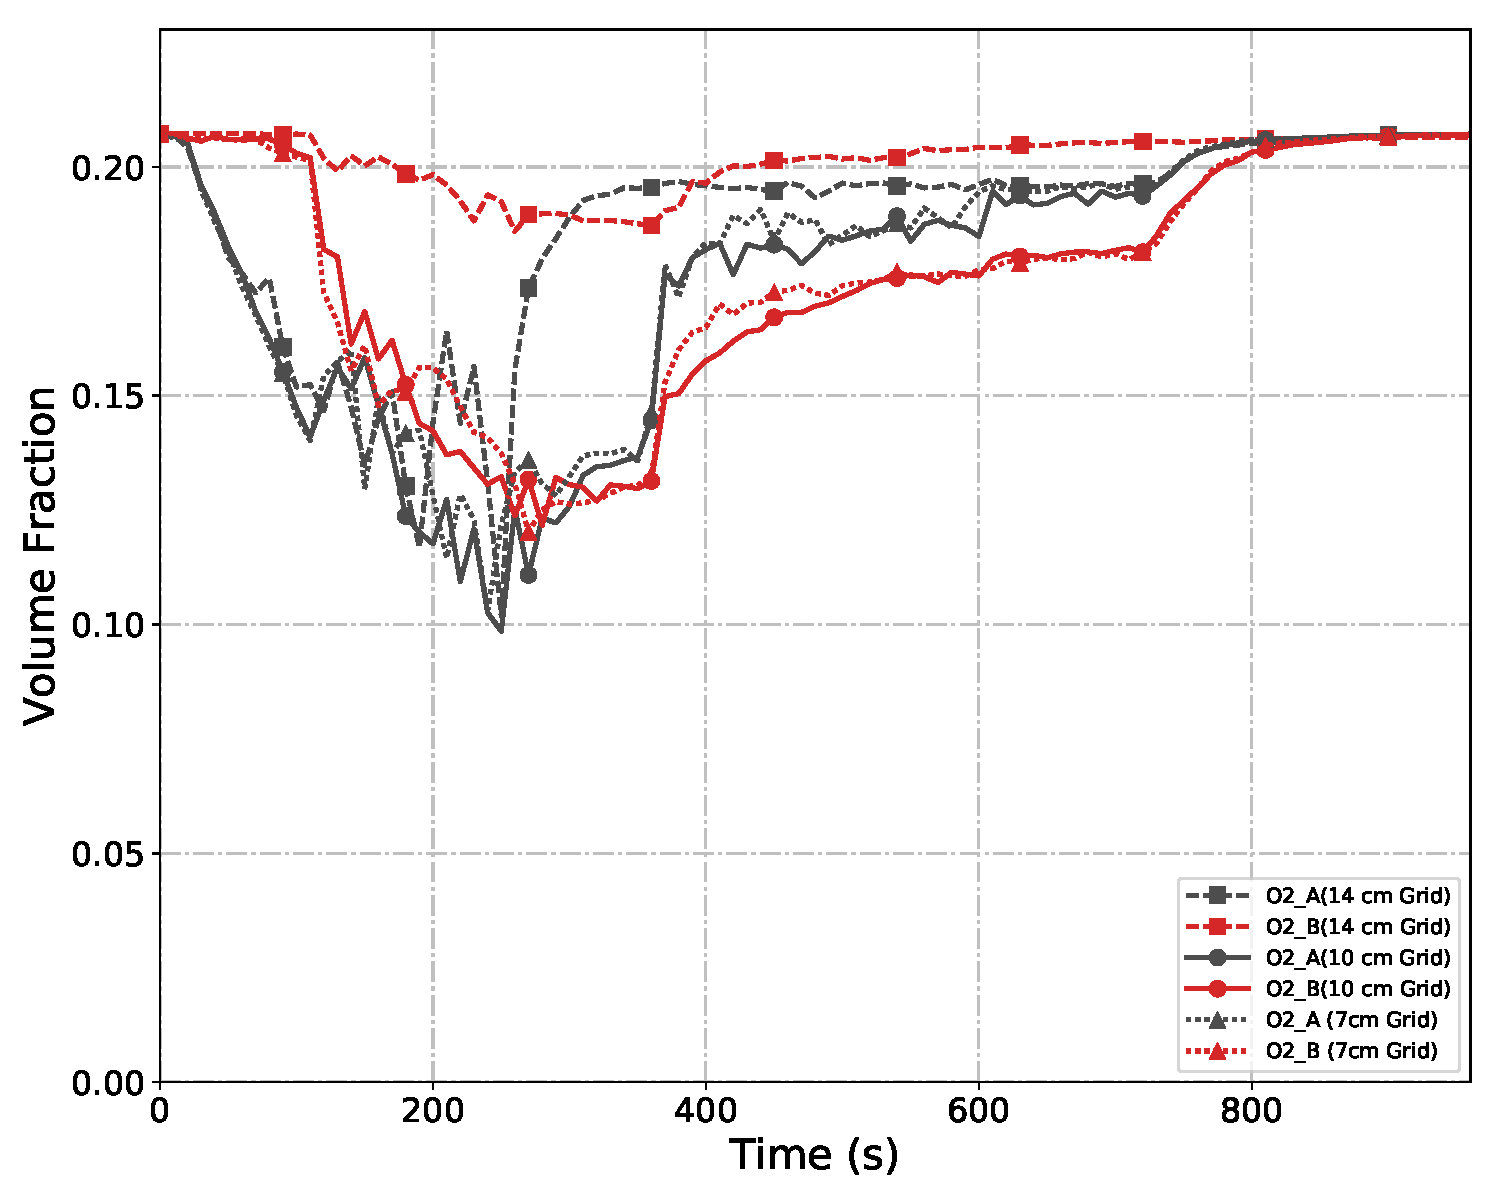
\includegraphics[width=\columnwidth]{Figures/Plots/Grid_Sensitivity/Gas_Concentration/Test_25_O2}
	\caption[$O_2$ concentrations for West Structure simulation with different grid cell sizes.]{$O_2$ concentrations output by the FDS simulation of Test~25 in the West Structure using three different grid cell sizes.}
	\label{fig:west_O2_sensitivity}
\end{figure}

\begin{figure}[!h]
	\centering
	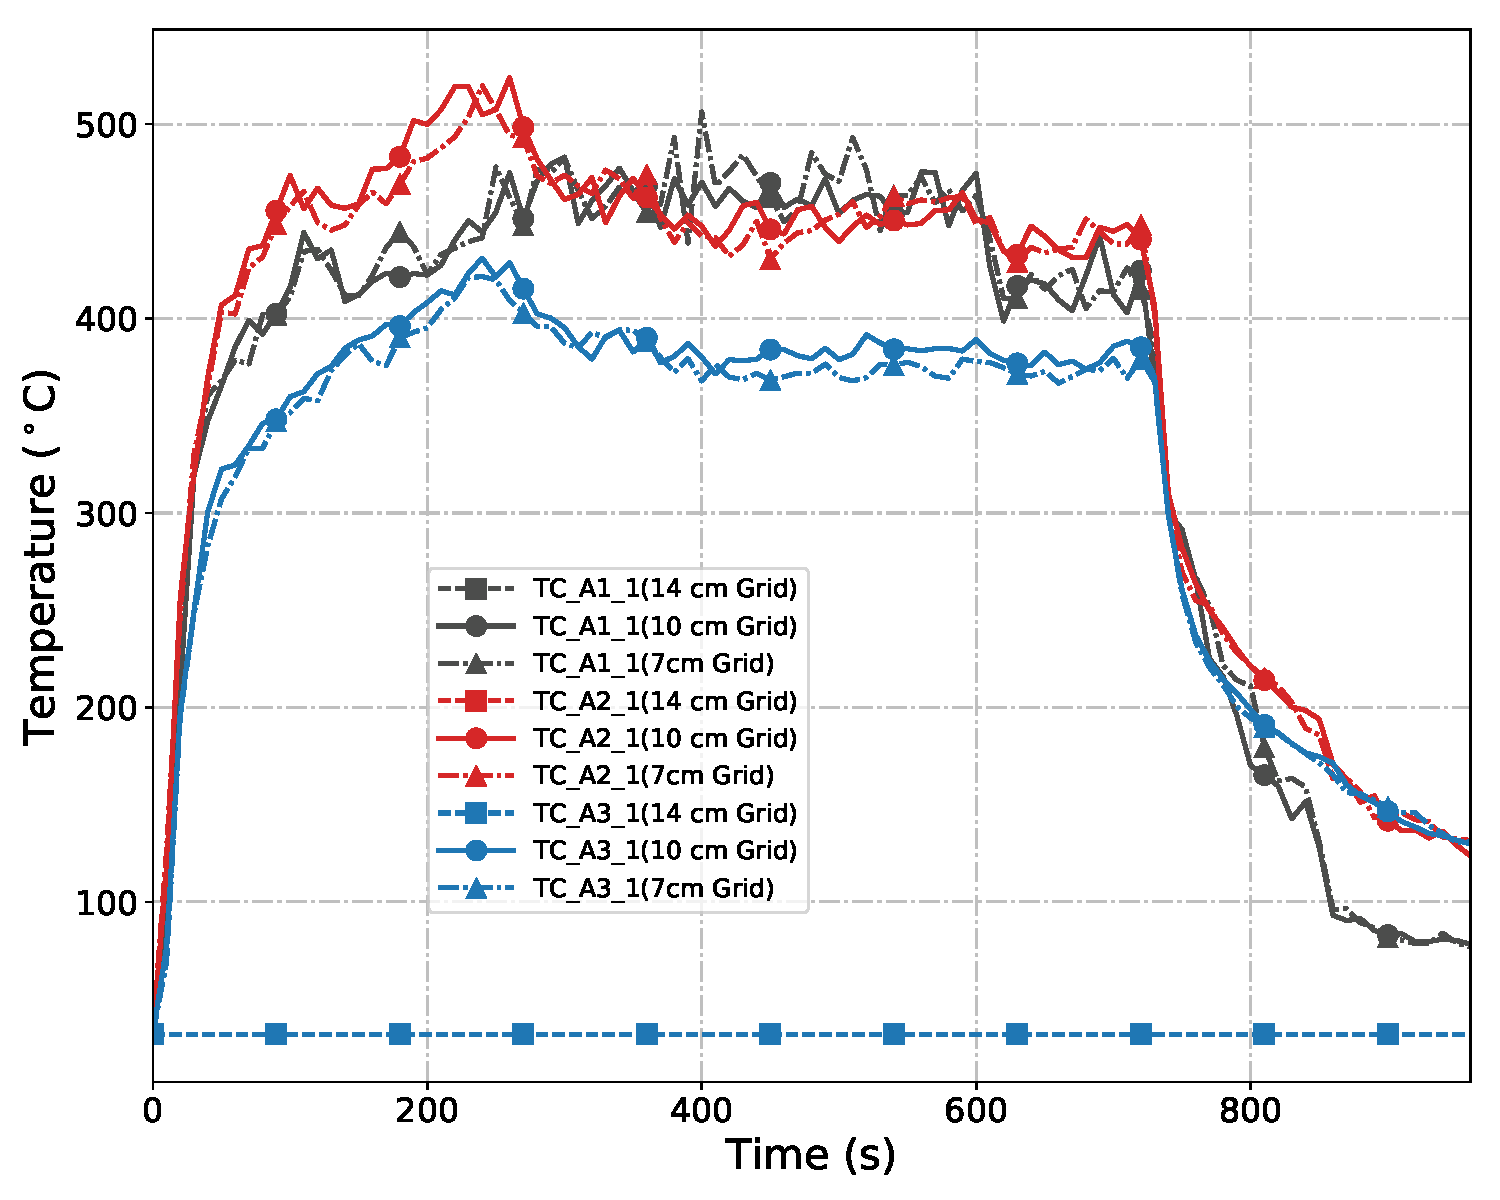
\includegraphics[width=0.87\columnwidth]{Figures/Plots/Grid_Sensitivity/Temperature/Test_25_cjet_1}
	\\~\\
	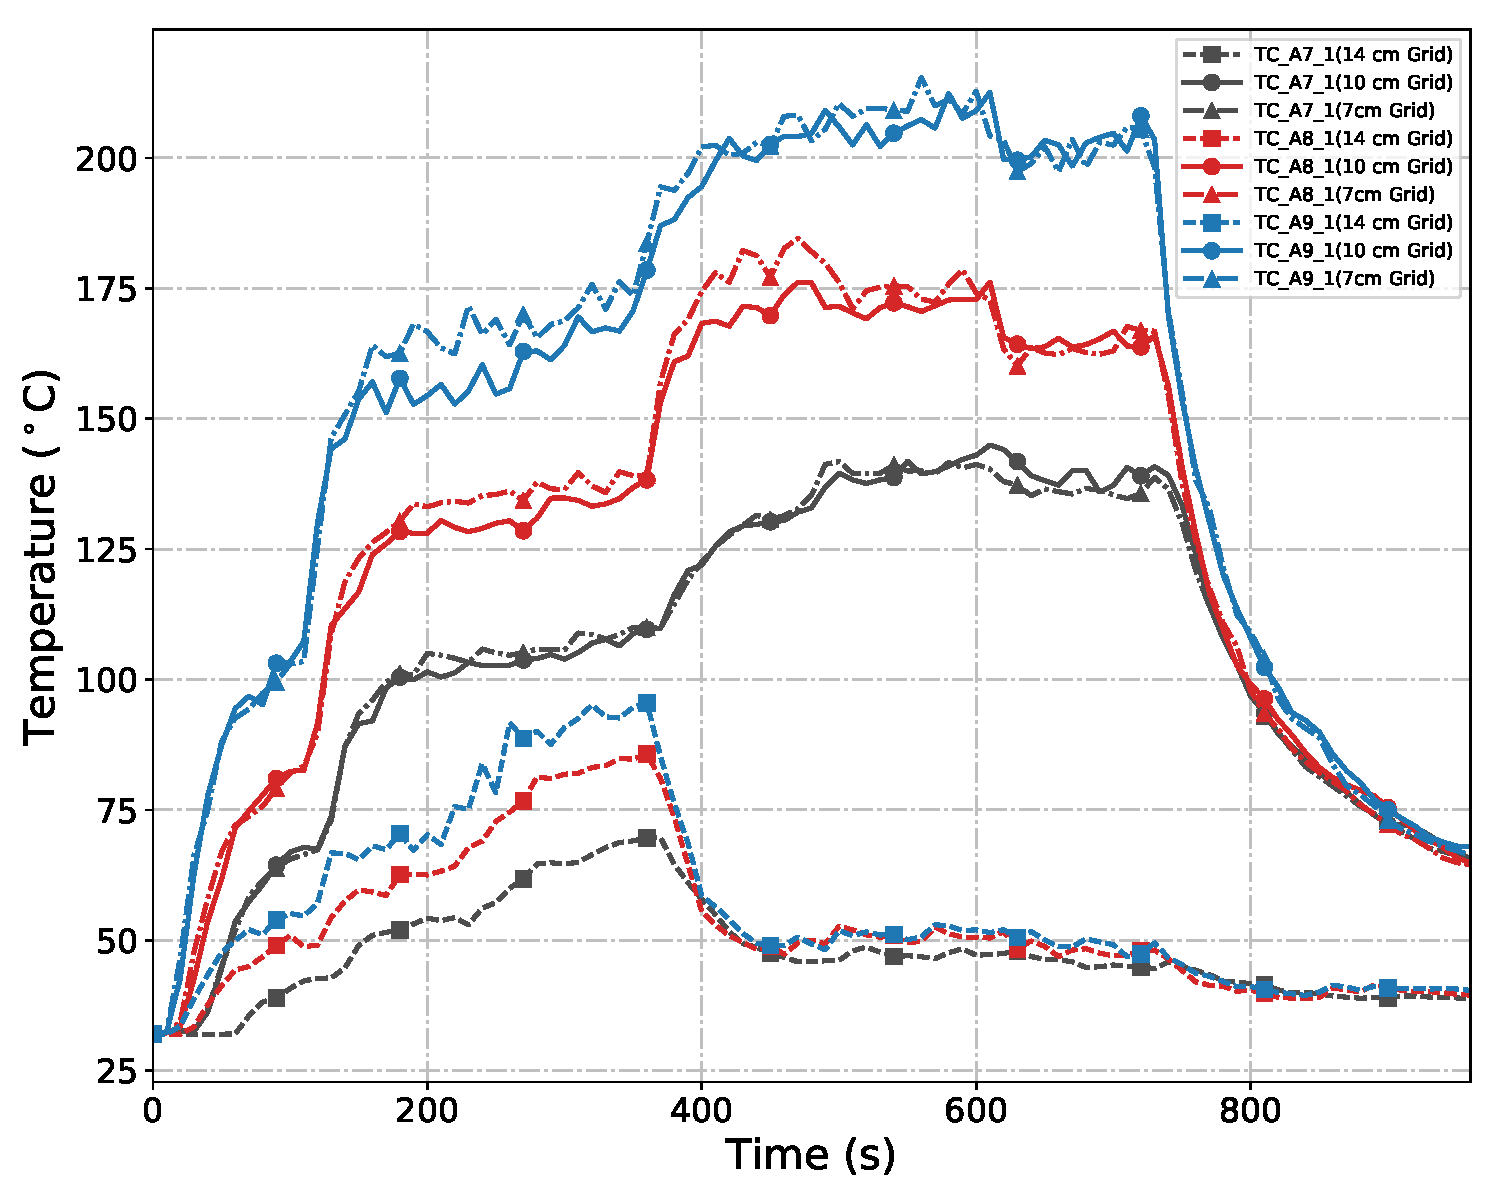
\includegraphics[width=0.87\columnwidth]{Figures/Plots/Grid_Sensitivity/Temperature/Test_25_cjet_2}
	\caption[Ceiling jet temperatures for West Structure simulation with different grid cell sizes.]{Ceiling jet temperatures output by the FDS simulation of Test~25 in the West Structure using three different grid cell sizes.}
	\label{fig:west_cjet_sensitivity}
\end{figure}

\FloatBarrier

The plots presented above show that significant differences occur at various times between the model data produced using the coarse grid and the same model data produced using the medium and fine grid resolutions. For example, looking at Figure~\ref{fig:west_O2_sensitivity}, the oxygen volume fraction data on the first floor of the West Structure output by the coarse grid deviates significantly from the data produced by medium and fine grid sizes around 300 seconds. Furthermore, the oxygen volume fraction data on the second floor output using the coarse grid drops to a minimum of approximately 0.18 during the portion of the simulation in which the burners are ignited, while the volume fraction data output using the medium and fine grids drop to a similar minimum that is around 0.13. 

Looking at the oxygen volume fraction and ceiling jet temperature data output by the East Structure simulation, Figures~\ref{fig:east_O2_sensitivity} and \ref{fig:east_cjet_sensitivity}, respectively, for different mesh resolutions, the data from the coarse grid exhibits more agreement with the medium and fine grid data than the West Structure simulation data plots. However, significant differences still arise between the coarse grid data and the simulation data produced by the medium and fine resolutions, such as the larger decline in ceiling jet temperature seen around 400~seconds.   

% Notice in Figure~\ref{fig:west_cjet_sensitivity}, the 14~cm grid was not refined enough to define the thermocouple locations at 0.03~m below the ceiling. 
Due to the large discrepancies between the coarse grid data and the data produced by the other two mesh resolutions, the coarse grid was considered too coarse for all simulations of the burner experiments. However, there doesn't appear to be any significant differences between the simulation data produced by the medium mesh resolution and the simulation data produced by the fine mesh resolution. As a result, the medium grid cell size of 10~cm was selected for all nine FDS simulations.

\section{FDS Model Data Compared to Experimental Data}
In the following subsections, the temperature, gas species concentration, gas velocity, and heat flux measurements predicted by the FDS simulations are compared to the corresponding sensor data measured during the propane burner experiments. Two different types of graphs are included to aid in the comparison of the model data and experimental data. The first type is similar to the mesh sensitivity study figures in that it shows the simulation data and experimental data (time-averaged over 10~seconds) plotted over the duration of an experiment for a specific data type at a specific location(s). Only one plot is presented for each discussed data quantity; the remaining figures of the discussed data types plotted over the duration each experiment for the different measurement locations are included in Appendix~\ref{chap:exp_FDS_plots}.

The second type of figure presented with each data quantity discussion summarizes the model uncertainty in predicting the specific data quantity. The summary graphs are similar to those presented in the FDS Validation Guide~\cite{FDS_Validation_Guide} --- each is a log/log scatter plot in which the $x$ value of each point is based on a set of measured, experimental data and the $y$ value of each point is based on the equivalent set of predicted data from the FDS simulation. No data from Tests~2--4 were used to generate the summary scatter plots because the heat release rates prescribed to the FDS simulations of the tests were determined through the use of a correlation (MQH) based on the experimental temperature data instead of through a direct physical measurement, such as the flow rate of propane to the burners used to determine the prescribed heat release rates for the other six simulations. The procedure used to generate the scatter plots and statistical data is briefly outlined below. Full details of the analysis are described in detail in by McGrattan and Toman in Ref.~\cite{McGrattan:Metrologia}.

Taking $M_i$ and $E_i$ to represent the change in the value of a quantity from its ambient at a specific time based on the data output by the FDS simulation and measured by instrumentation during the experiment, respectively, the mean and standard deviation of the distribution can be estimated by first calculating
\begin{equation} 
	\overline{\ln(M/E)}=\frac{1}{n} \sum_{i=1}^n \ln\left( \frac{M_i}{E_i} \right)
\end{equation}
Note, the natural logarithm function is used so that the variance of the random variable can be expressed in terms of the relative uncertainty. The assumption that $\ln(M/E)$ is normally distributed has been tested for each data type of interest by the developers of FDS, and the results are shown in the FDS Validation Guide. The standard deviation of the logarithm of a normally distributed random variable is approximately equal to the standard deviation divided by its mean, the relative standard deviation. The least squares estimate of the standard deviation of the combined distribution is defined as:
\begin{equation}
\label{eq:least_sqrs}
	\widetilde{\sigma}_m^2 + \widetilde{\sigma}_E^2 \approx \frac{1}{n-1}\sum_{i=1}^n \left[ \ln(M_i/E_i) - \overline{\ln(M/E)} \right]^2
\end{equation}
Using the pair of measured and predicted values with the known $\widetilde{\sigma}_E$, the expression on the right can be evaluated. Eq.~\ref{eq:least_sqrs} imposes a constraint on the experimental uncertainty value, $\widetilde{\sigma}_E$, and in combination with a second constraint that $\widetilde{\sigma}_M$ cannot be less than $\widetilde{\sigma}_E$ because it's impossible to show that the model is more accurate than the measurements against which it's compared, the following is produced:
\begin{equation}
	\widetilde{\sigma}_E^2 \leq \frac{1}{2}\textrm{Var}(\ln(M/E))
\end{equation}
Using the mean of the distribution, an estimate of a bias factor, $\delta$, which expresses the tendency of the model to over or under-predict the measured quantity, can be found:
\begin{equation}
	\delta \approx \exp\left( \overline{\ln(M/E)}+\frac{\widetilde{\sigma}_M^2}{2}-\frac{\widetilde{\sigma}_E^2}{2} \right)
\end{equation}

The values of $\delta$, $\sigma_M$, and $\sigma_E$ are reported with each log/log plot in the following sections. For each plot, the solid red line and solid black line represent the expected values for $M$ and $E$, respectively, and the dashed lines represent $\pm \sigma$, or standard deviations, of the data corresponding to the line color. Each plotted gray point represents an average value of the specific data quantity across a 30 second test period in which one or more gas burners were ignited and only natural ventilation was present throughout the structure (i.e., no PPV fan was turned on). All the points are based on computed values over the applicable time periods of Tests~5--6 and Tests~22--25. Table~\ref{table:stats_compare} in the final section of this chapter summarizes the statistical values calculated for each data type and is presented with a brief discussion of how the values compare to the same statistical values listed in the FDS Validation Guide.

\subsection{Temperature}

\subsubsection*{\textit{Hot Gas Layer}}
A quantity that is commonly estimated for compartment fire scenarios is the location of the interface between the hot, smoke-laden upper layer and cooler, lower layer. Some fire models, such as two-zone models, calculate this value directly, along with the average temperature of the hot gas (upper) layer and lower layer. Being that it's a CFD model, FDS computes a continuous profile of temperature and as such, does not directly calculate the interface location or the average temperature of each layer. However, numerous techniques exist to estimate the layer height and average temperatures from a continuous vertical profile of temperature. The temperatures measured by the thermocouples in the vertical arrays throughout the experimental structures were used to define a vertical profile of temperature, $T(z)$, in which $z$ is the height above the floor ($z=0$ at the floor and $z=H$ at the room's ceiling). Then, the vertical temperature profile was used to estimate the hot gas layer (HGL) temperature by a method developed by Janssens and Tran~\cite{Janssens:JFS1992}. Taking $T_u$ as the upper layer temperature, $T_l$ as the lower layer temperature, and $z_{int}$ as the HGL interface height, the method is outlined below, starting with the calculation of the quantities $I_1$ and $I_2$
\begin{equation*}
	I_1 = \int^H_0 T(z)dz = (H-z_{int})T_u+z_{int}T_l
\end{equation*}
\begin{equation*}
	I_2 = \int^H_0 \frac{1}{T(z)}dz = (H-z_{int})\frac{1}{T_u}+z_{int}\frac{1}{T_l}
\end{equation*}
$I_1$ and $I_2$ are then used to solve for $z_{int}$ as follows:
\begin{equation}
	z_{int}=\frac{T_l(I_1I_2-H^2)}{I_1+I_2 T_l^2-2T_l H}
\end{equation}
where $T_l$ is the temperature in the lowest mesh cell (or thermocouple) and $T_u$ is the average upper layer temperature defined by
\begin{equation}
	(H-z_{int})T_u=\int^H_{z_{int}} T(z)dz
\end{equation}

Figure~\ref{fig:HGL_data} contains the HGL temperature derived from experimental data plotted with the HGL temperature derived from the FDS simulation data over the duration of Test~22. The log/log scatter plot comparing the HGL temperatures obtained from the predicted temperature data and the HGL temperatures obtained from the measured experimental data for the applicable time periods from all the tests is presented in Figure~\ref{fig:loglog_HGL}.

\begin{figure}[!h]
	\centering
	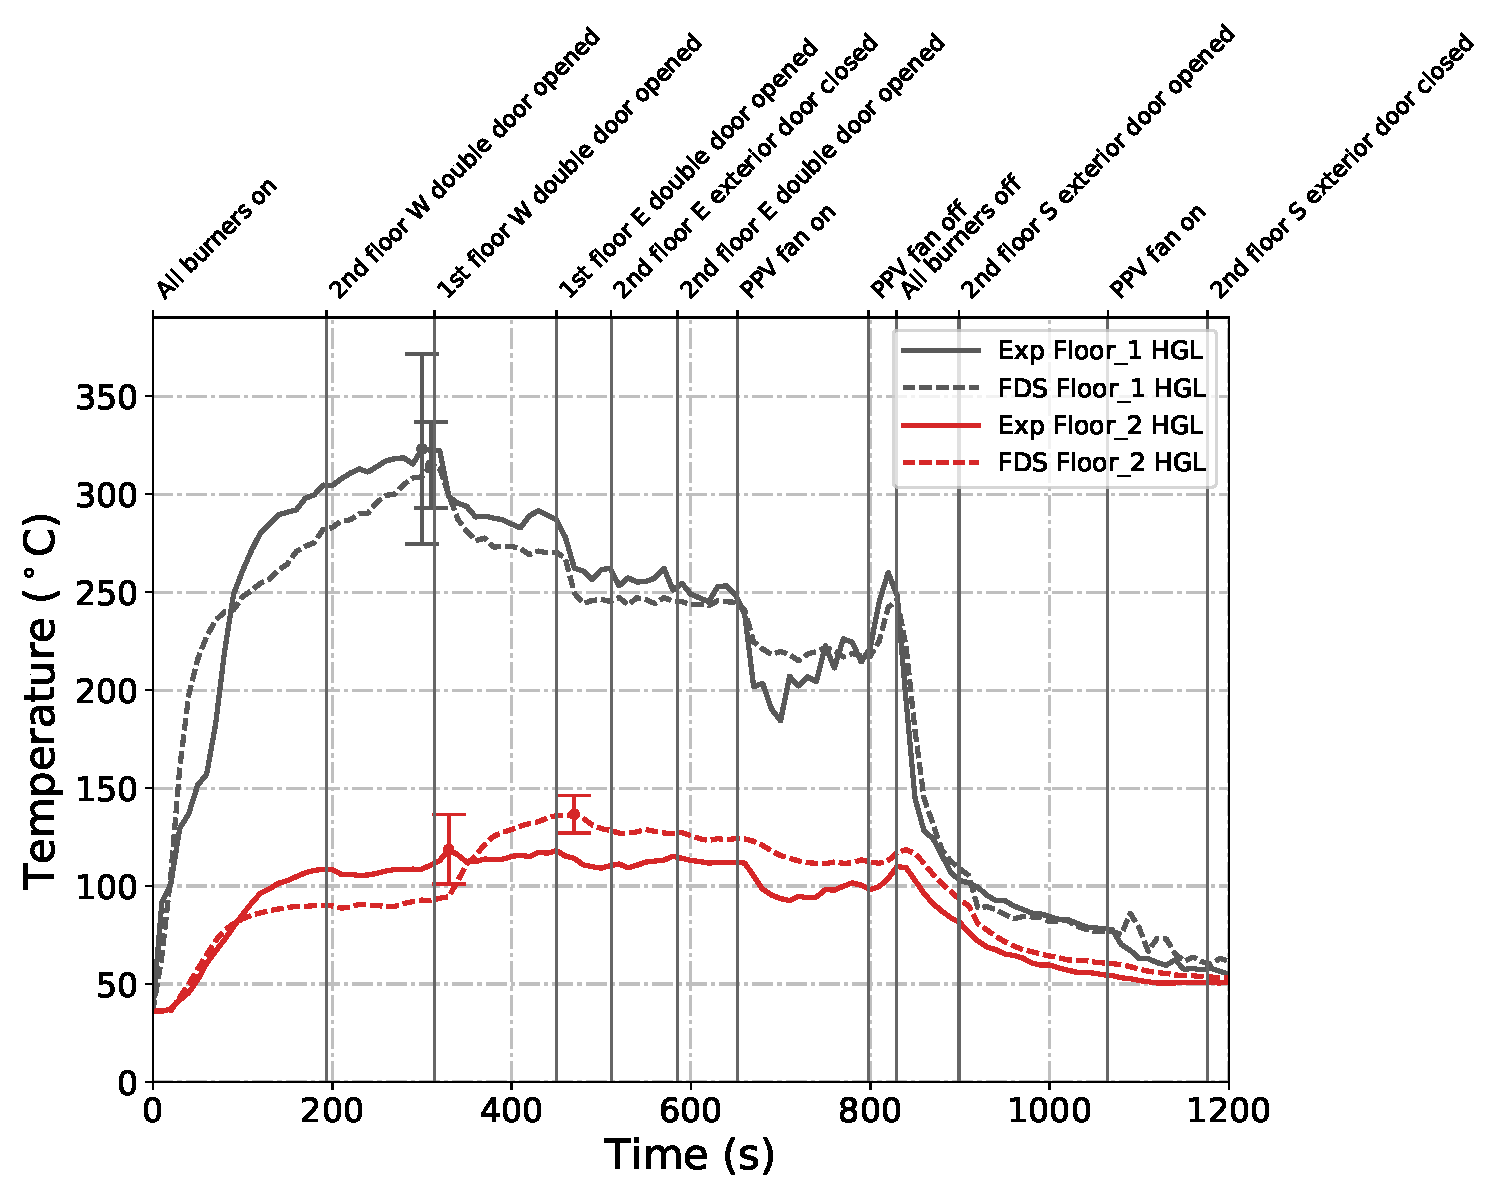
\includegraphics[width=\columnwidth]{Figures/Plots/Validation/Temperature/Test_22_HGL}
	\caption[Plots of measured and predicted hot gas layer temperatures during Test~22.]{Plots of measured and predicted hot gas layer temperatures on the first and second floors of the West Structure during Test~22.}
	\label{fig:HGL_data}
\end{figure}

\begin{figure}[!h]
	\centering
	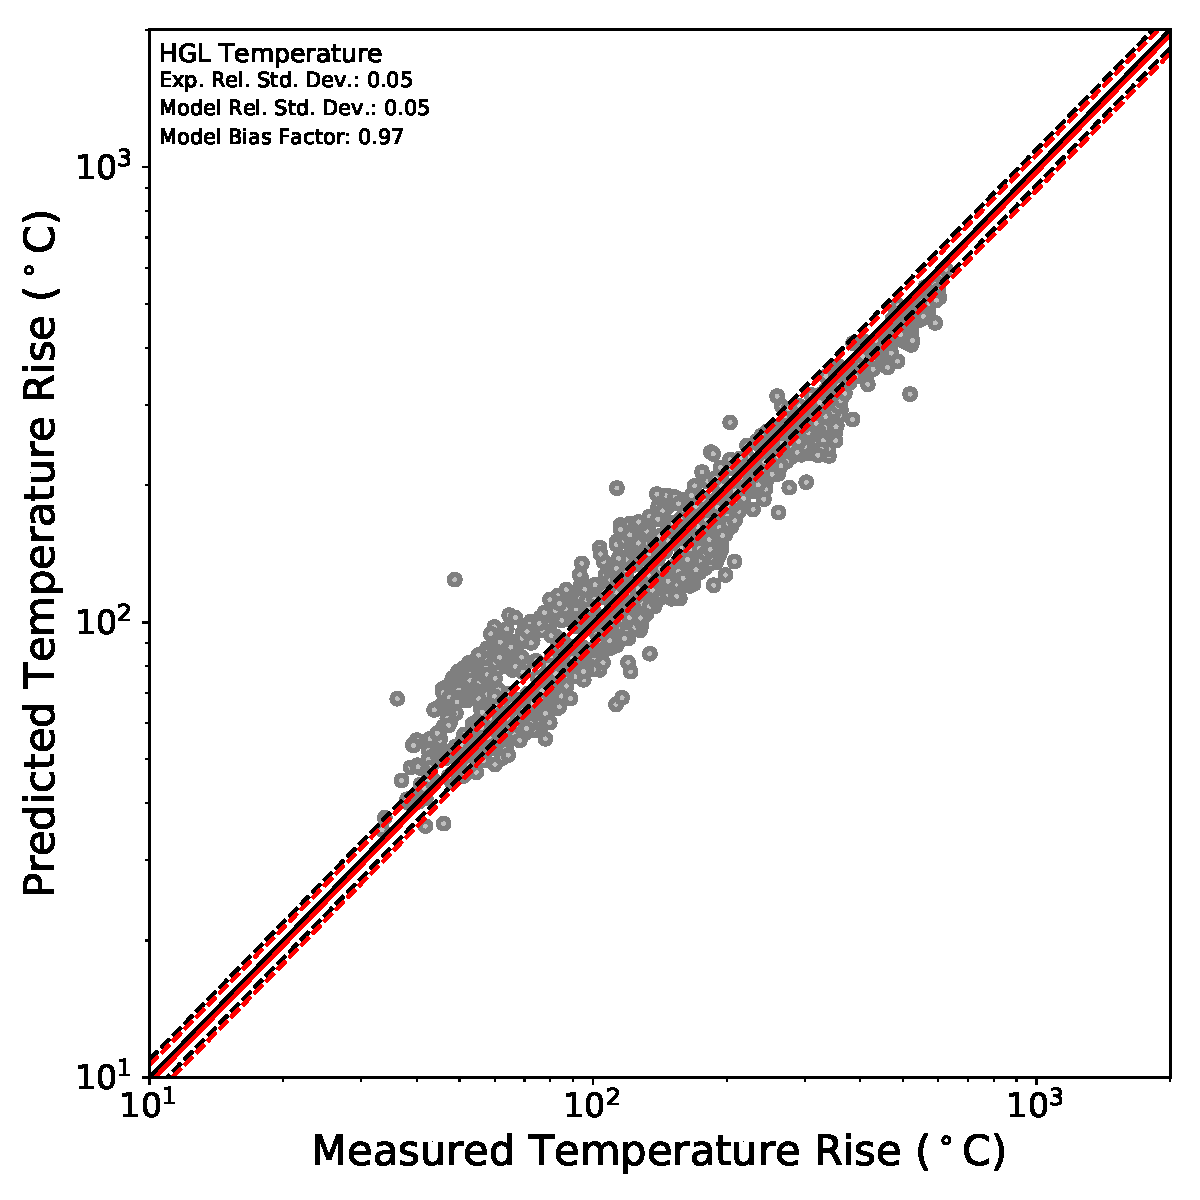
\includegraphics[width=\columnwidth]{Figures/Plots/Validation/Temperature/loglog_HGL}
	\caption{Summary of measured and predicted hot gas layer temperatures.}
	\label{fig:loglog_HGL}
\end{figure}

\FloatBarrier
\subsubsection*{\textit{Ceiling Jet}}
The temperature near the ceiling, often referred to as the ceiling jet temperature, can be used to evaluate a model's ability to predict the activation times of sprinklers, smoke detectors, and other fire protection devices at ceiling height. The ``ceiling jet'' temperature discussed in this report refers to the temperature measured by the top thermocouple (closest to the ceiling) of the various thermocouple arrays located throughout the experimental structures. Figure~\ref{fig:cjet_data} shows the ceiling jet temperatures measured by the top thermocouple plotted with the ceiling jet temperatures predicted by the FDS model over the duration of Test~4. Figure~\ref{fig:loglog_cjets} contains the log/log scatter plot of the ceiling jet temperatures predicted by the FDS simulations compared to the corresponding measured ceiling jet temperatures for all applicable time periods in Tests~5--6 and Tests~22--25.
\begin{figure}[!h]
	\centering
	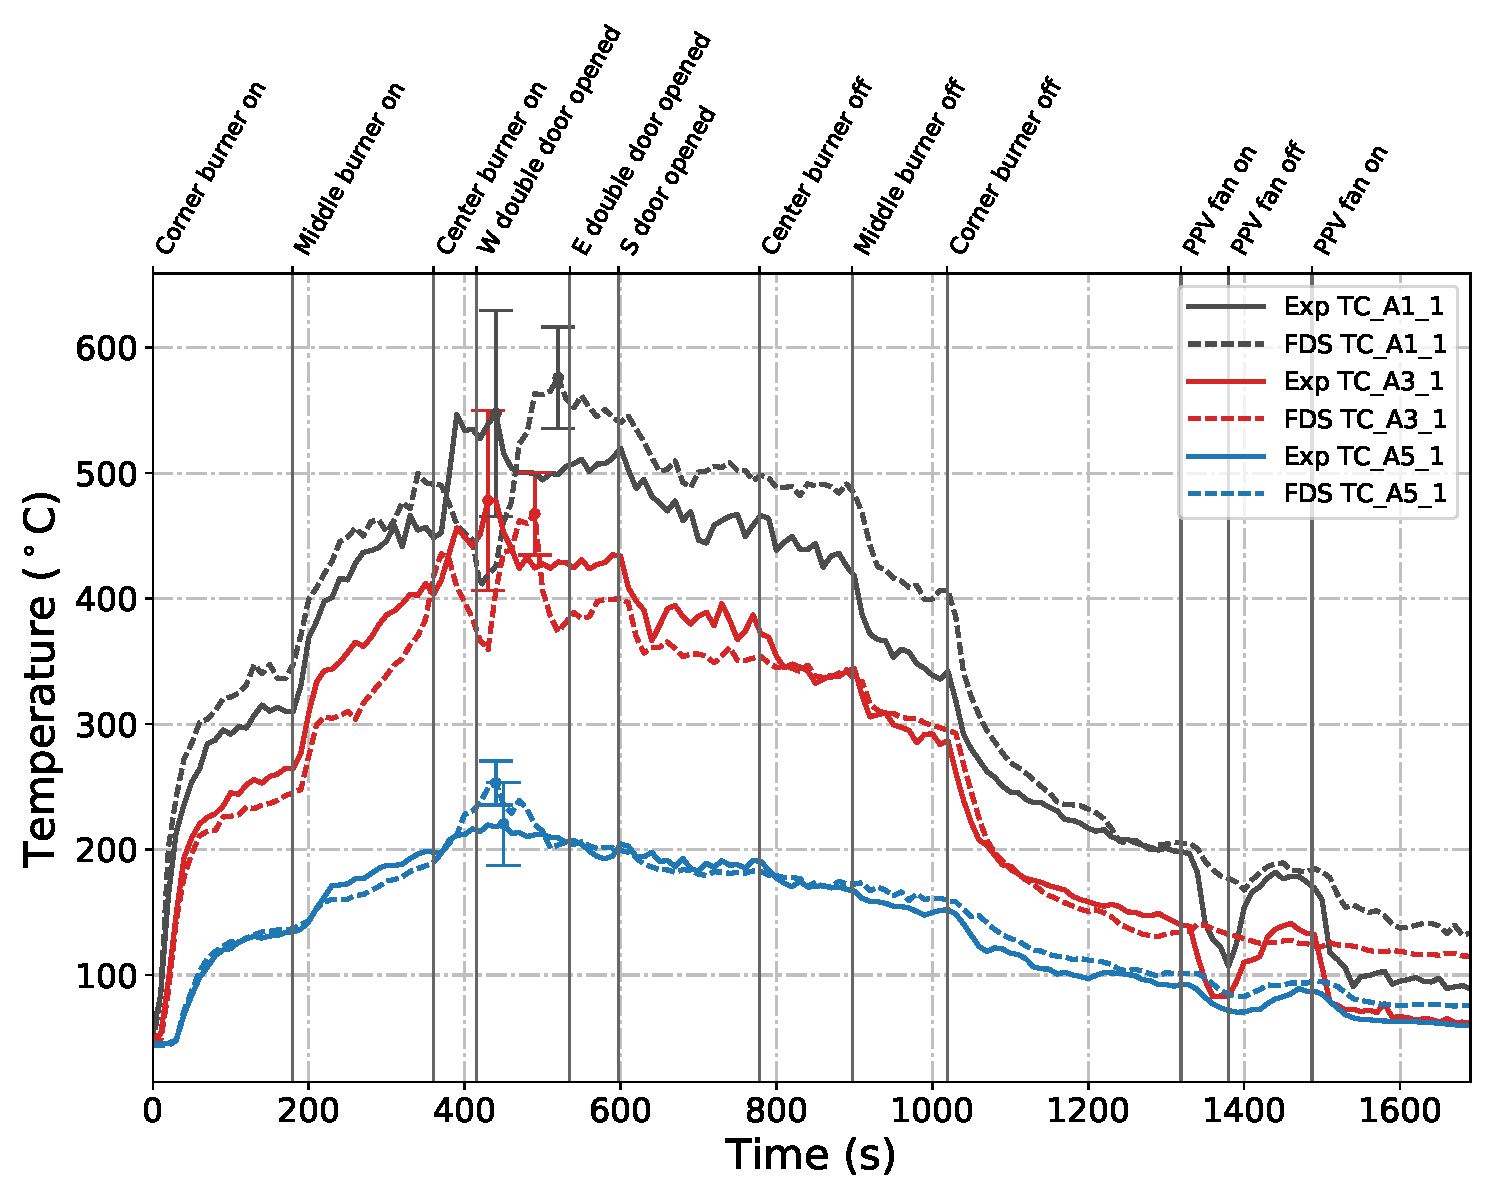
\includegraphics[width=\columnwidth]{Figures/Plots/Validation/Temperature/Test_4_cjet_1}
	\caption[Plots of measured and predicted ceiling jet temperatures during Test~4.]{Plots of measured and predicted ceiling jet temperatures during Test~4 obtained from thermocouple arrays A1, A3, and A5 located in the fire room, middle room, and north room, respectively, in the East Structure.}
	\label{fig:cjet_data}
\end{figure}

\begin{figure}[!h]
	\centering
	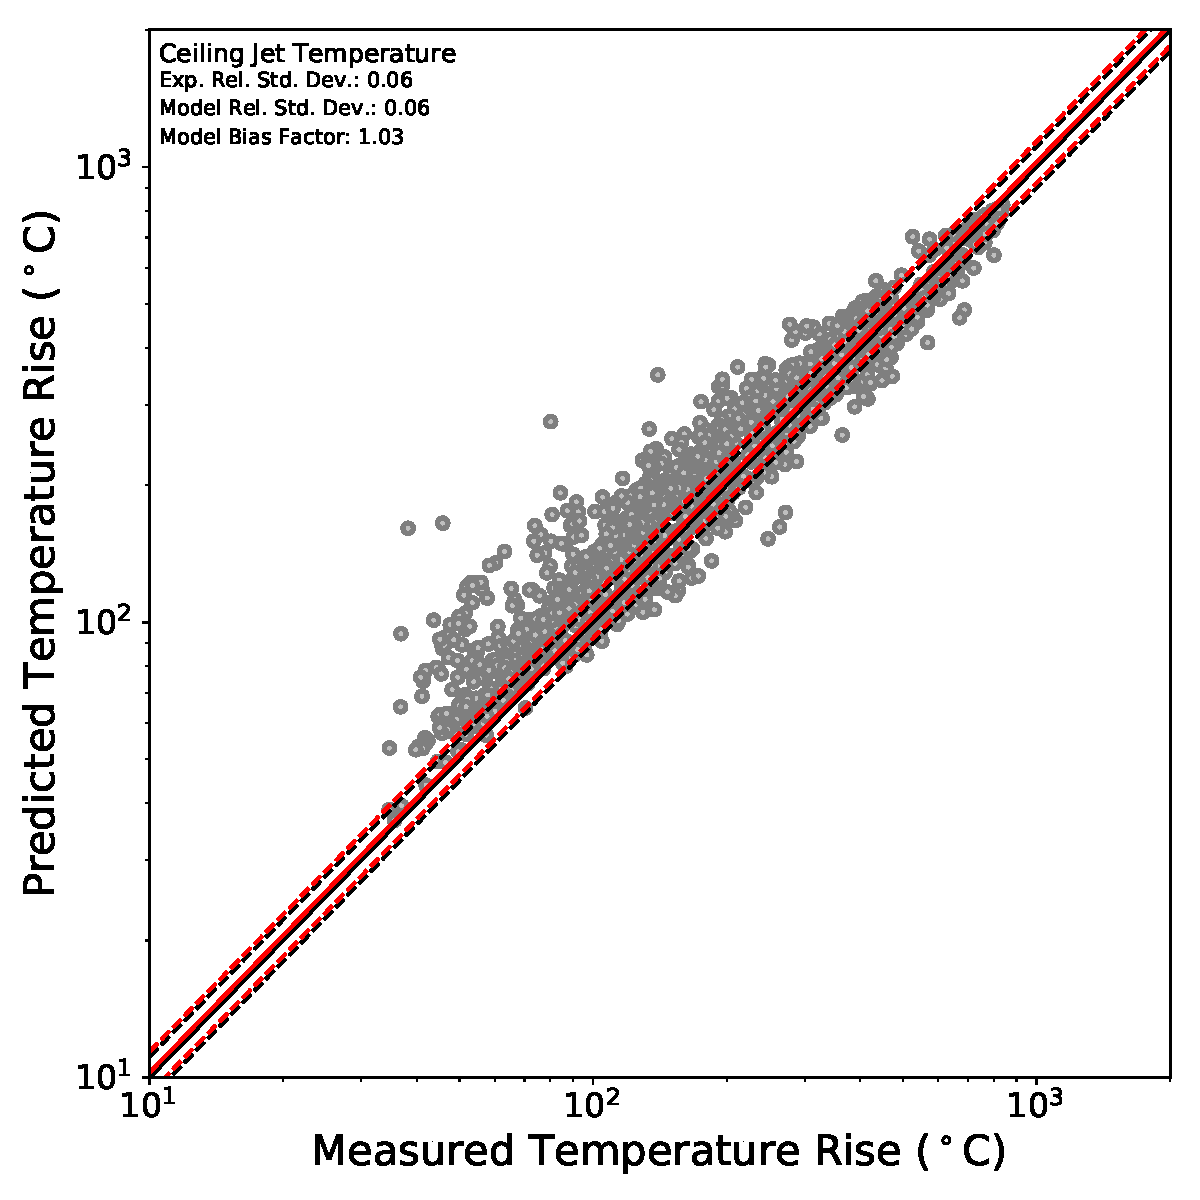
\includegraphics[width=\columnwidth]{Figures/Plots/Validation/Temperature/loglog_cjetTCs}
	\caption{Summary of measured and predicted ceiling jet temperatures.}
	\label{fig:loglog_cjets}
\end{figure}

\clearpage
\subsubsection*{\textit{Thermocouple Arrays}}
In addition to the HGL and ceiling jet temperatures, the measured and predicted temperatures at each individual thermocouple in the various thermocouple arrays were compared. Two figures of the temperatures over the duration of each test were generated for each thermocouple array: one of the ``upper'' temperatures corresponding to the temperatures from the four thermocouples closest to the ceiling and another of the ``lower'' temperatures corresponding to the other four thermocouples, the four closest to the floor. Figure~\ref{fig:TCarray_data} contains the measured and predicted upper temperatures from array A1 over the duration of Test~24 and Figure~\ref{fig:loglog_TC_arrays} shows the log/log scatter plot of the temperatures measured at the different thermocouple locations within the thermocouple arrays compared to the temperatures at the same locations predicted by the FDS simulations for Tests~5--6 and Tests~22--25.
\begin{figure}[!h]
	\centering
	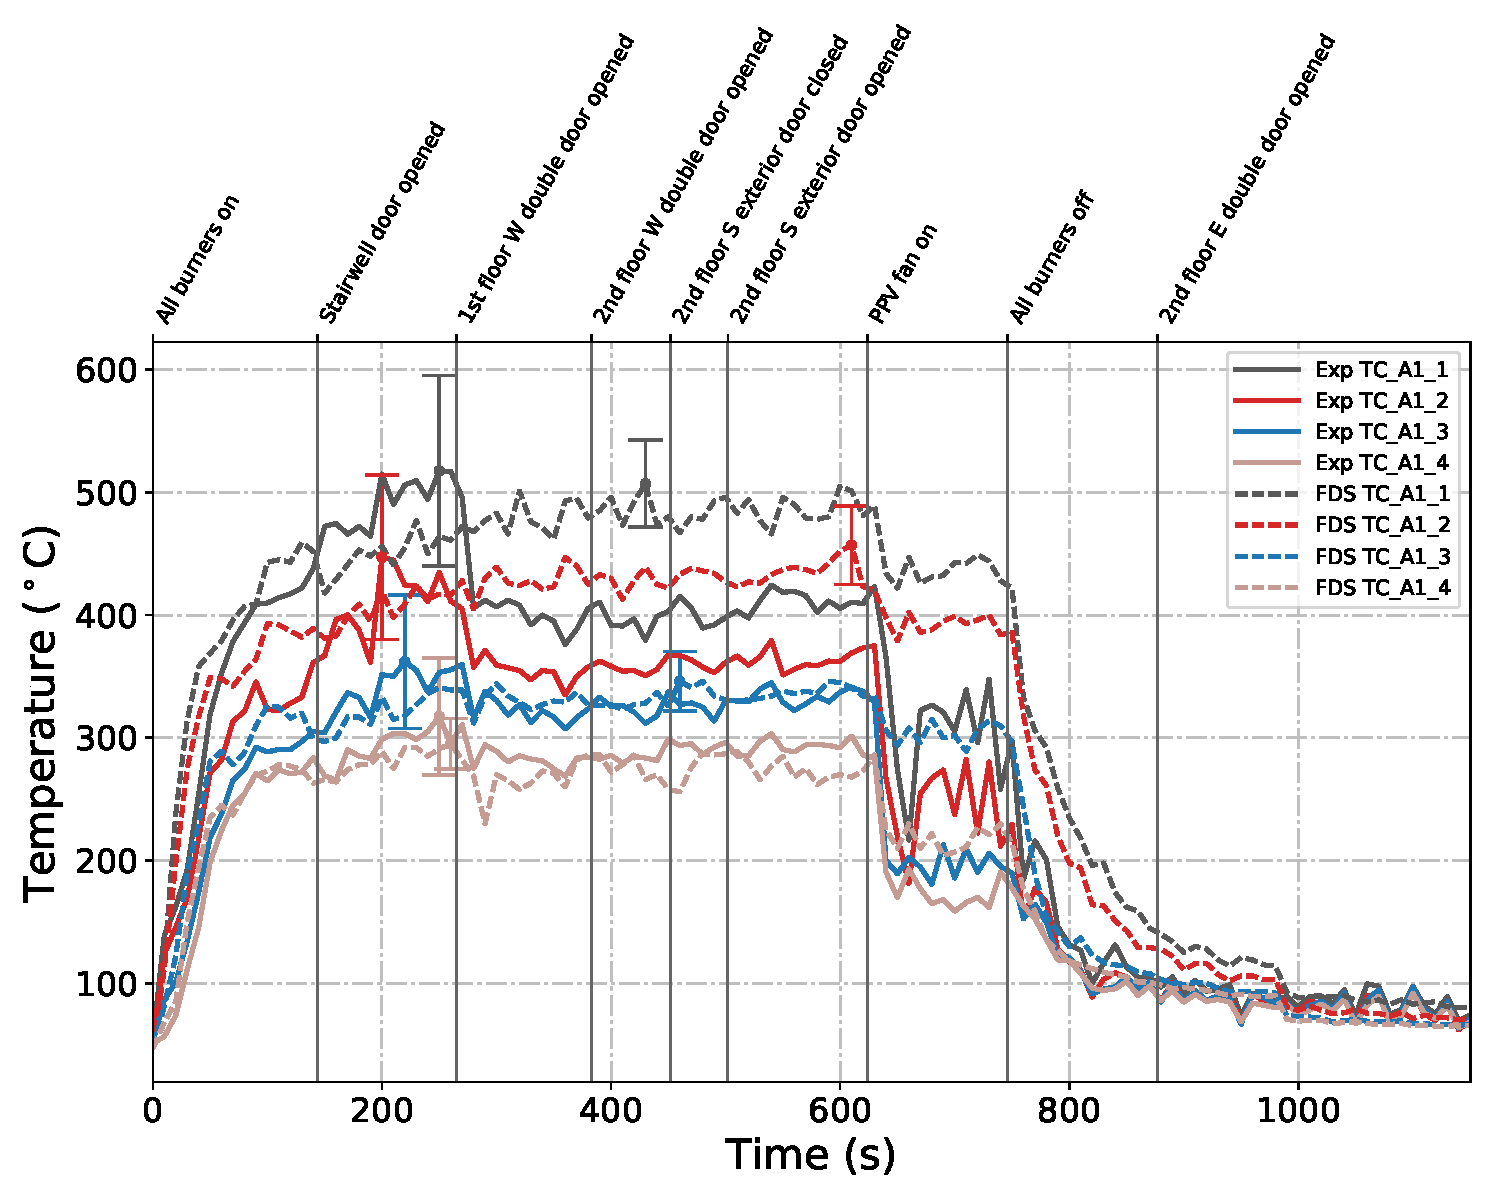
\includegraphics[width=\columnwidth]{Figures/Plots/Validation/Temperature/Test_24_TC_A1_upper}
	\caption[Plot of the measured and predicted upper temperatures from array A1 during Test~24.]{Plots of measured and predicted ``upper'' temperatures from array A1 during Test~24 in the West Structure.}
	\label{fig:TCarray_data}
\end{figure}

\begin{figure}[!h]
	\centering
	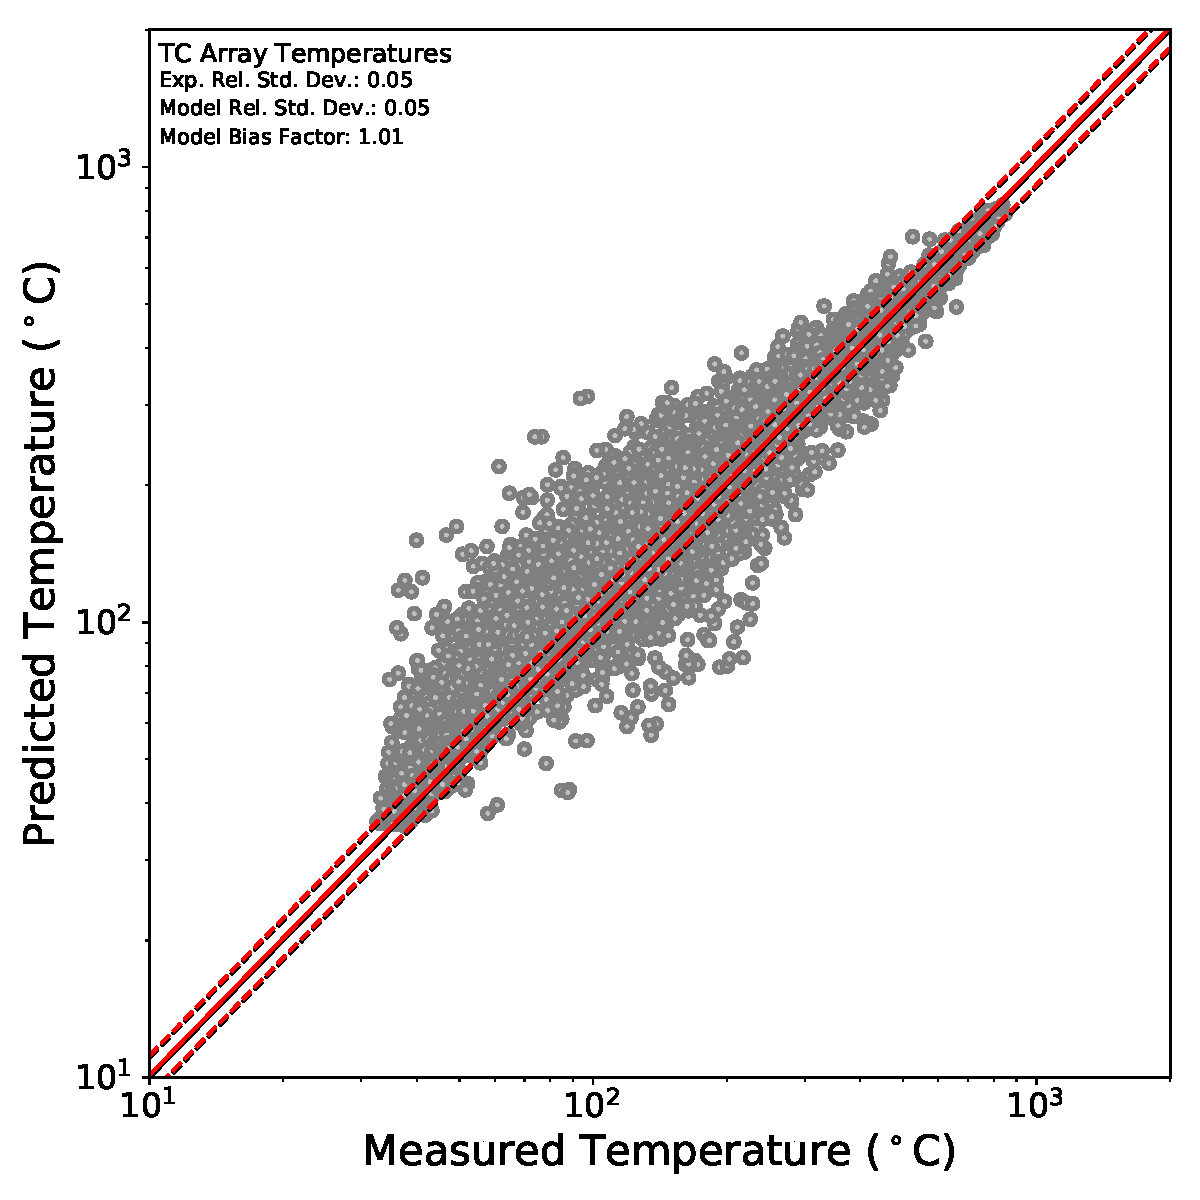
\includegraphics[width=\columnwidth]{Figures/Plots/Validation/Temperature/loglog_TC_arrays}
	\caption{Summary of measured and predicted temperatures at the individual thermocouple locations within the different thermocouple arrays.}
	\label{fig:loglog_TC_arrays}
\end{figure}

\clearpage
\subsection{Gas Species Concentration}
\subsubsection*{\textit{$O_2$} Concentration}
The measured and predicted oxygen concentrations in the fire room and north room of the East Structure are plotted over the duration of Test~3 below in Figure~\ref{fig:Test3_O2}. Additionally, the summary log/log scatter plot of the predicted oxygen concentrations compared to the corresponding measured oxygen concentrations for the applicable time periods during Tests~5--6 and Tests~22--25 is shown in Figure~\ref{fig:loglog_O2}.
\begin{figure}[!h]
	\centering
	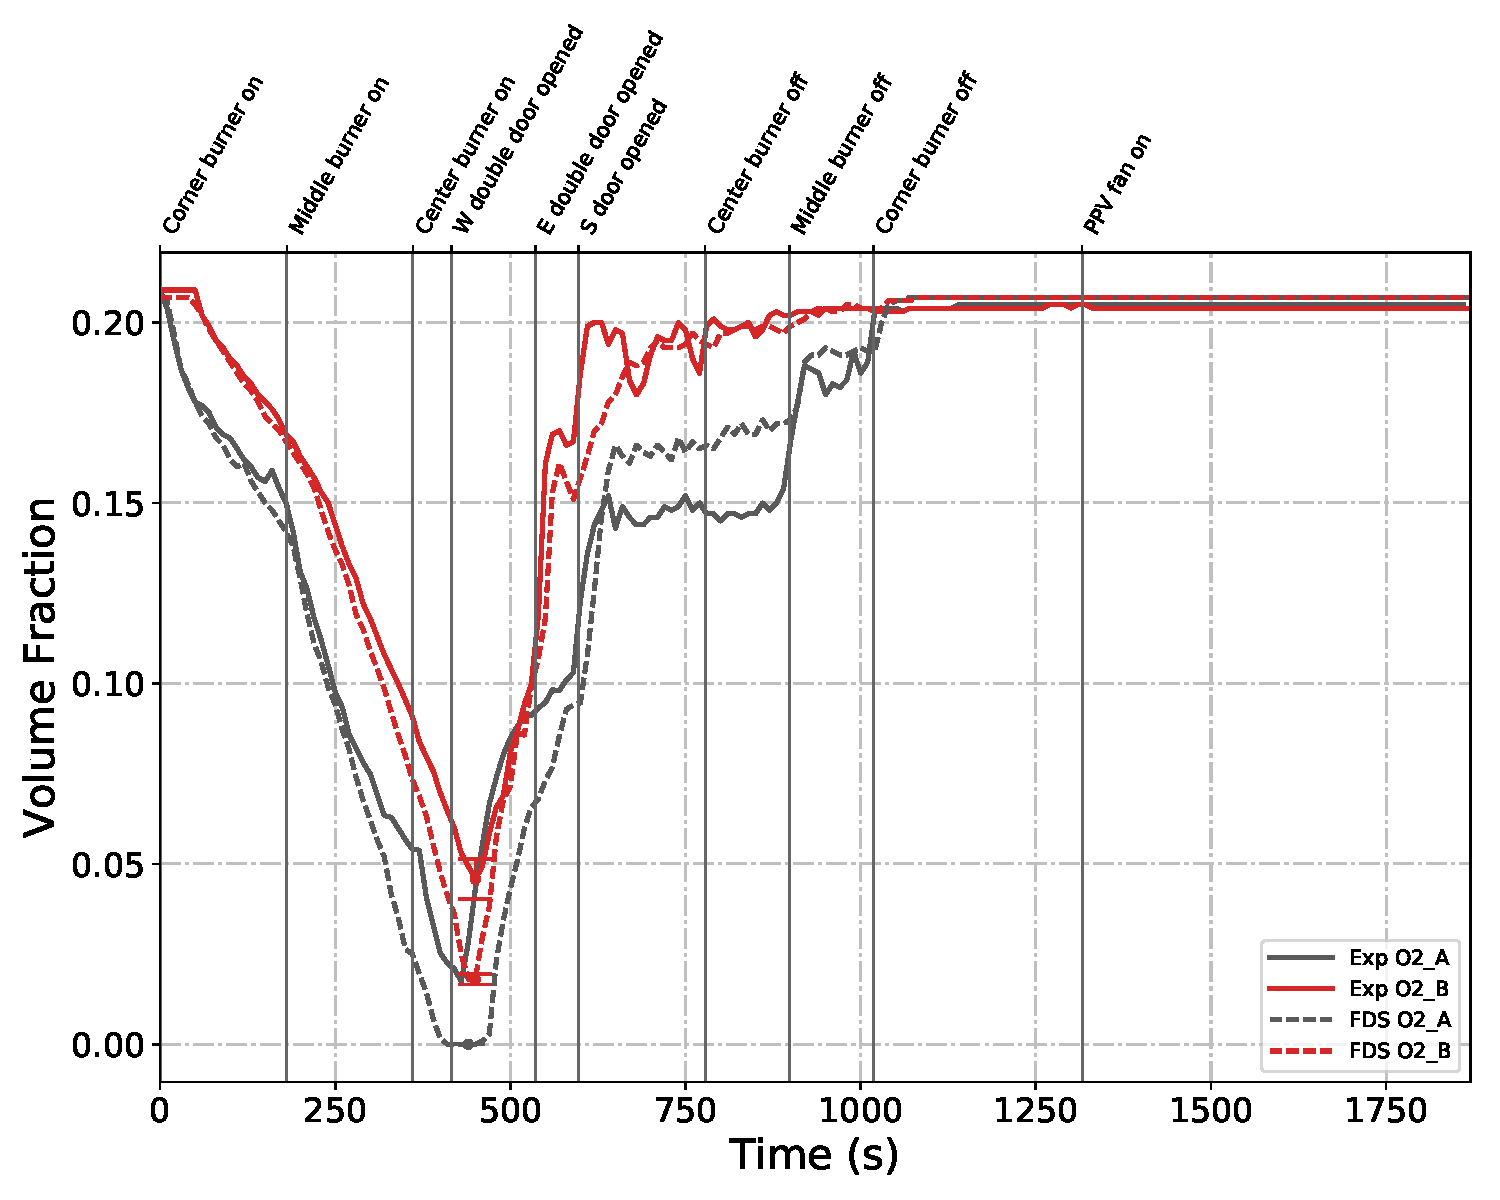
\includegraphics[width=\columnwidth]{Figures/Plots/Validation/Gas_Concentration/Test_3_O2}
	\caption[Plots of measured and predicted $O_2$ concentration during Test~3.]{Plots of measured and predicted $O_2$ concentrations in the fire room (black plots) and north room (red plots) of the East Structure during Test~3.}
	\label{fig:Test3_O2}
\end{figure}

\begin{figure}[!h]
	\centering
	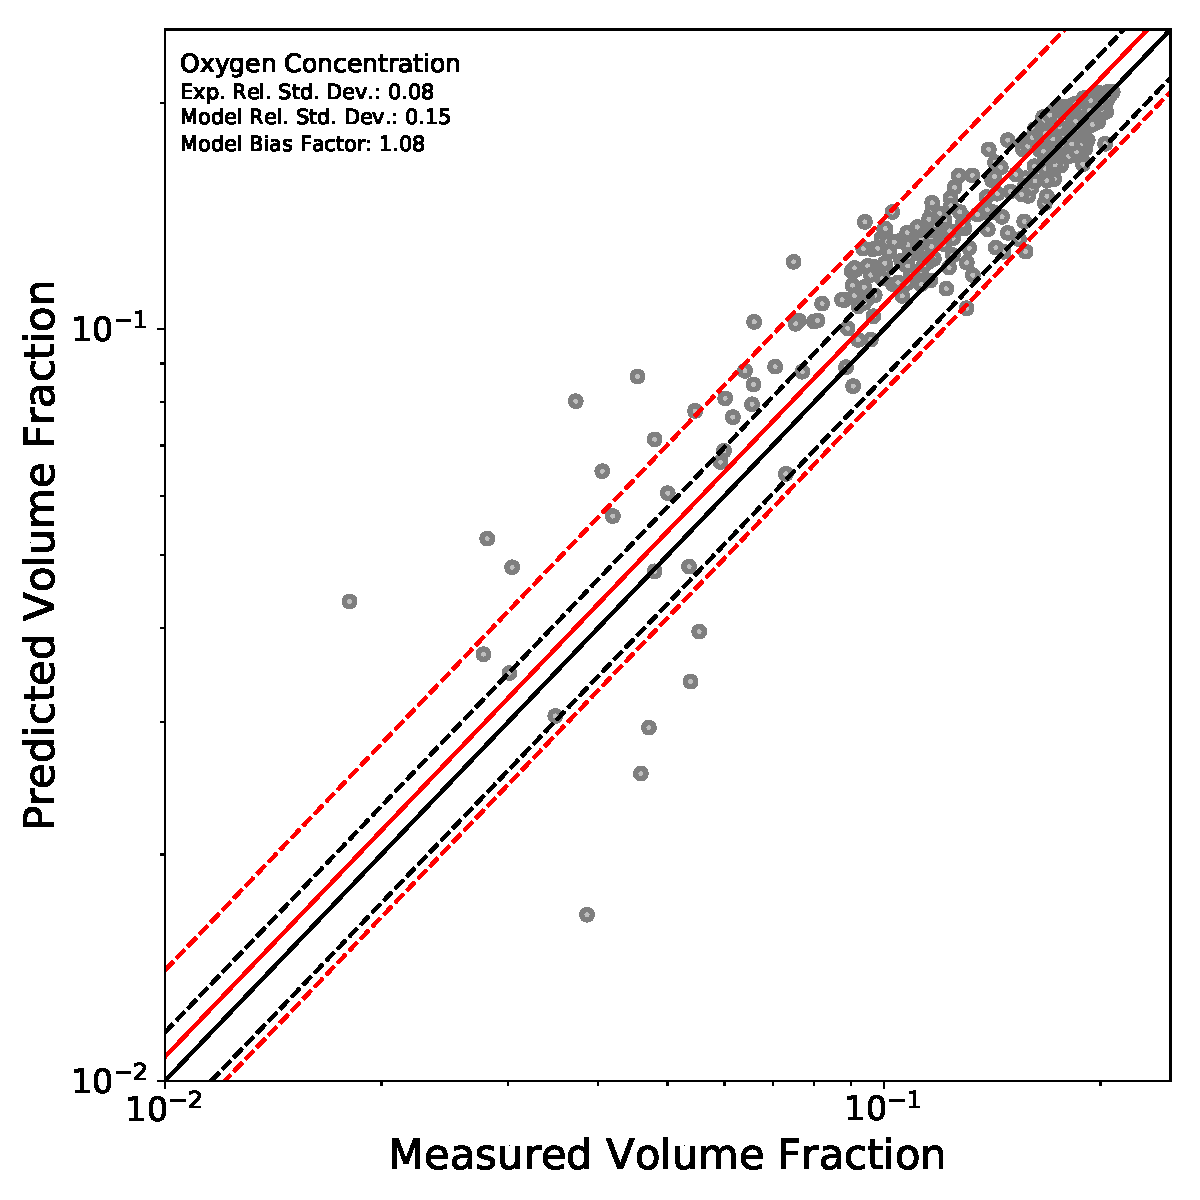
\includegraphics[width=\columnwidth]{Figures/Plots/Validation/Gas_Concentration/loglog_O2}
	\caption{Summary of measured and predicted $O_2$ concentrations.}
	\label{fig:loglog_O2}
\end{figure}

\clearpage
\subsubsection*{\textit{$CO_2$} Concentration}
The measured and predicted carbon dioxide concentrations in the fire room and north room of the East Structure are plotted over the duration of Test~3 below in Figure~\ref{fig:Test3_CO2}. The system used to measure the carbon dioxide concentrations could only measure carbon dioxide concentrations up to a maximum of 0.10. Thus, data pairs from the applicable time ranges of Tests~5--6 and Tests~22--25 for which the measured $CO_2$ volume fraction was 0.10 were not used to create the summary log/log scatter plot of the predicted $CO_2$ concentrations compared to the corresponding measured concentrations shown in Figure~\ref{fig:loglog_CO2} below.

\begin{figure}[!h]
	\centering
	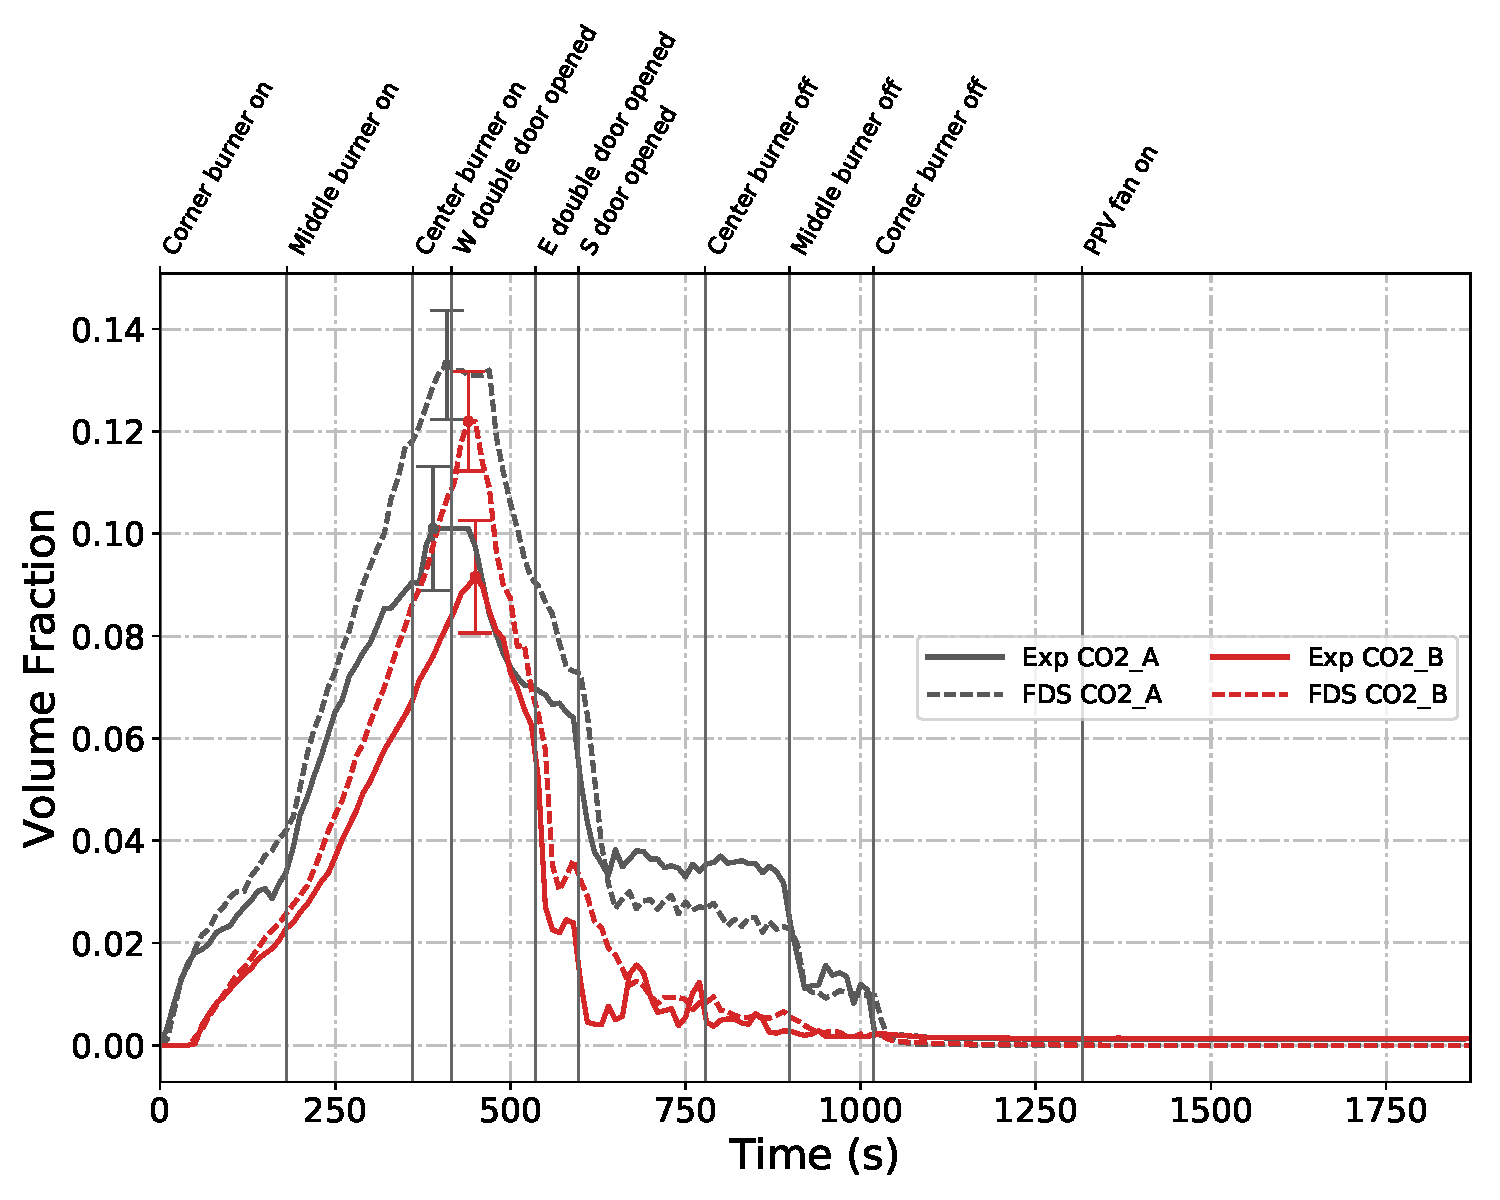
\includegraphics[width=\columnwidth]{Figures/Plots/Validation/Gas_Concentration/Test_3_CO2}
	\caption[Plots of measured and predicted $CO_2$ concentration during Test~3.]{Plots of measured and predicted $CO_2$ concentration in the fire room (black plots) and north room (red plots) of the East Structure during Test~3.}
	\label{fig:Test3_CO2}
\end{figure}

\begin{figure}[!h]
	\centering
	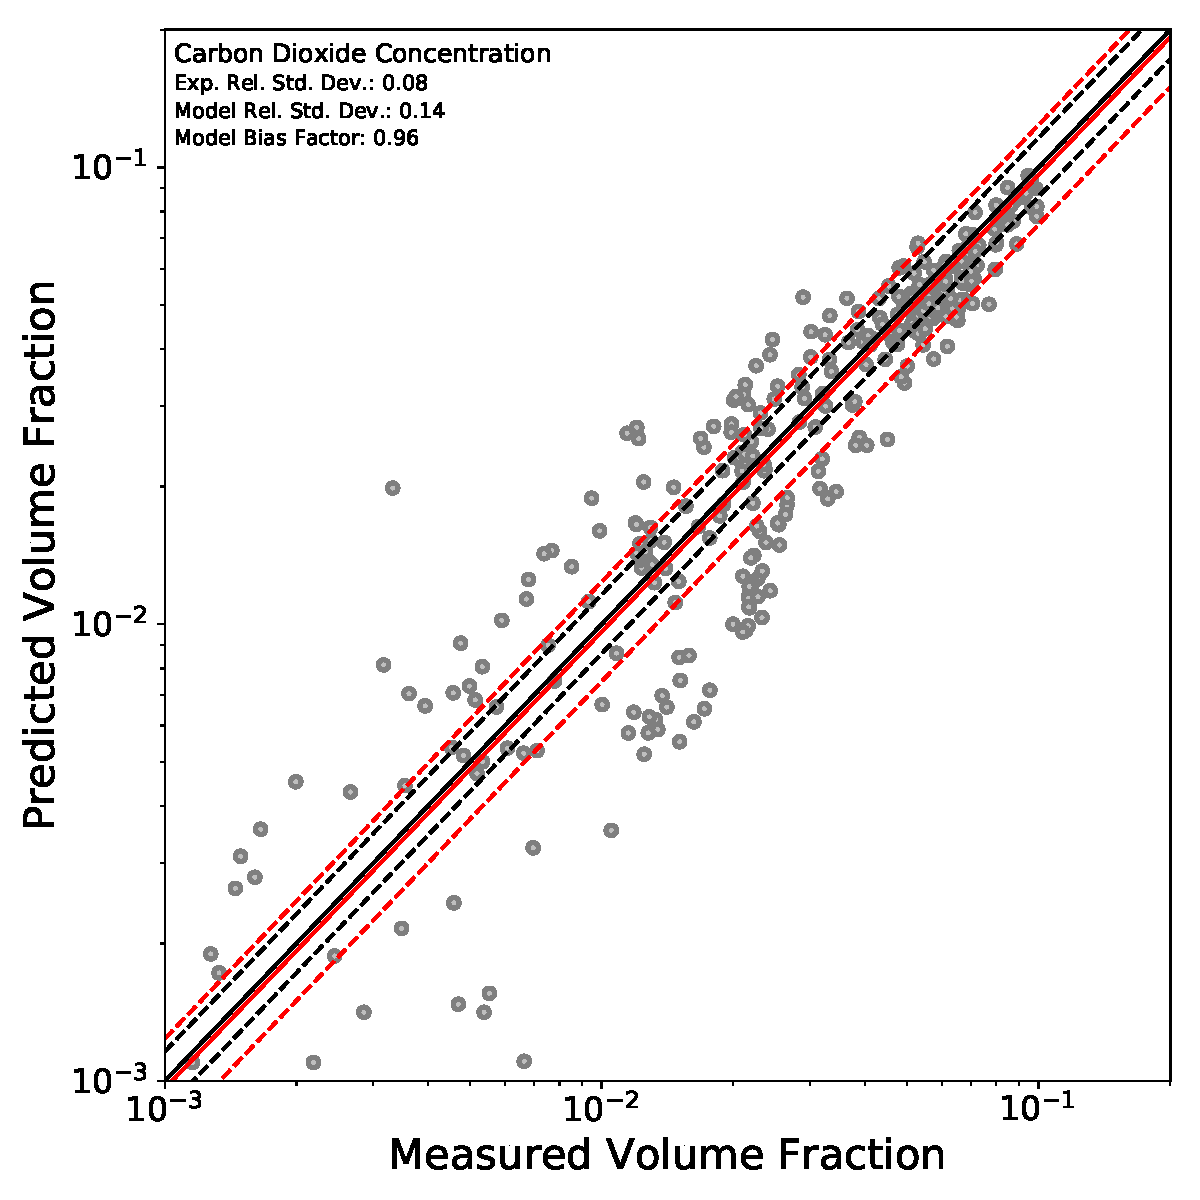
\includegraphics[width=\columnwidth]{Figures/Plots/Validation/Gas_Concentration/loglog_CO2}
	\caption{Summary of measured and predicted $CO_2$ concentrations.}
	\label{fig:loglog_CO2}
\end{figure}

\clearpage
\subsection{Gas Velocity}
Because the gas burner experiments were conducted outdoors, they were subject to environmental conditions, such as wind. To minimize the effect such environmental conditions could have on the analysis of the results, the only gas velocity measurements that are compared to predicted data are those that were indoors, or well-protected from the exterior. 

The only set of BDPs in the East Structure that was well-protected from the effects of environmental conditions was the set at the roof vent, array A10. Tests~5 and 6 were the only East Structure tests that incorporated the roof vent as a ventilation opening. Figure~\ref{fig:Test5_BDPs} presented below contains the gas velocity data measured at each individual probe in array A10 and the predicted gas velocity data at the same locations plotted over the duration of Test~5.

There was also only one well-protected set of BDPs in the West Structure: the array of eight probes located at the stairway door, array A10. Because the array contained eight measurement locations, plots of the gas velocity data at A10 for each West Structure test were divided between two figures: one of the data from the ``upper'' BDPs corresponding to the four probes closest to the top of the doorway and another of the data from the ``lower'' BDPs corresponding to the other four probes, the four closest to the floor. 

At the start of Tests~5 and 6, the roof vent was closed and then opened as an event later during the test. Similarly, for Tests~24 and 25, the stairway door was initially closed and opened later in the test as an event. For Tests~22 and 23, the stairwell door was opened for the entire duration of the experiment. The data used to produce Figure~\ref{fig:loglog_BDPs}, the log/log scatter plot of the predicted and measured gas velocity data, were limited to the data from the applicable time periods in which airflow through the vent opening at A10 was unrestricted (i.e., when the roof vent or stairway door was opened).   

\begin{figure}[!h]
	\centering
	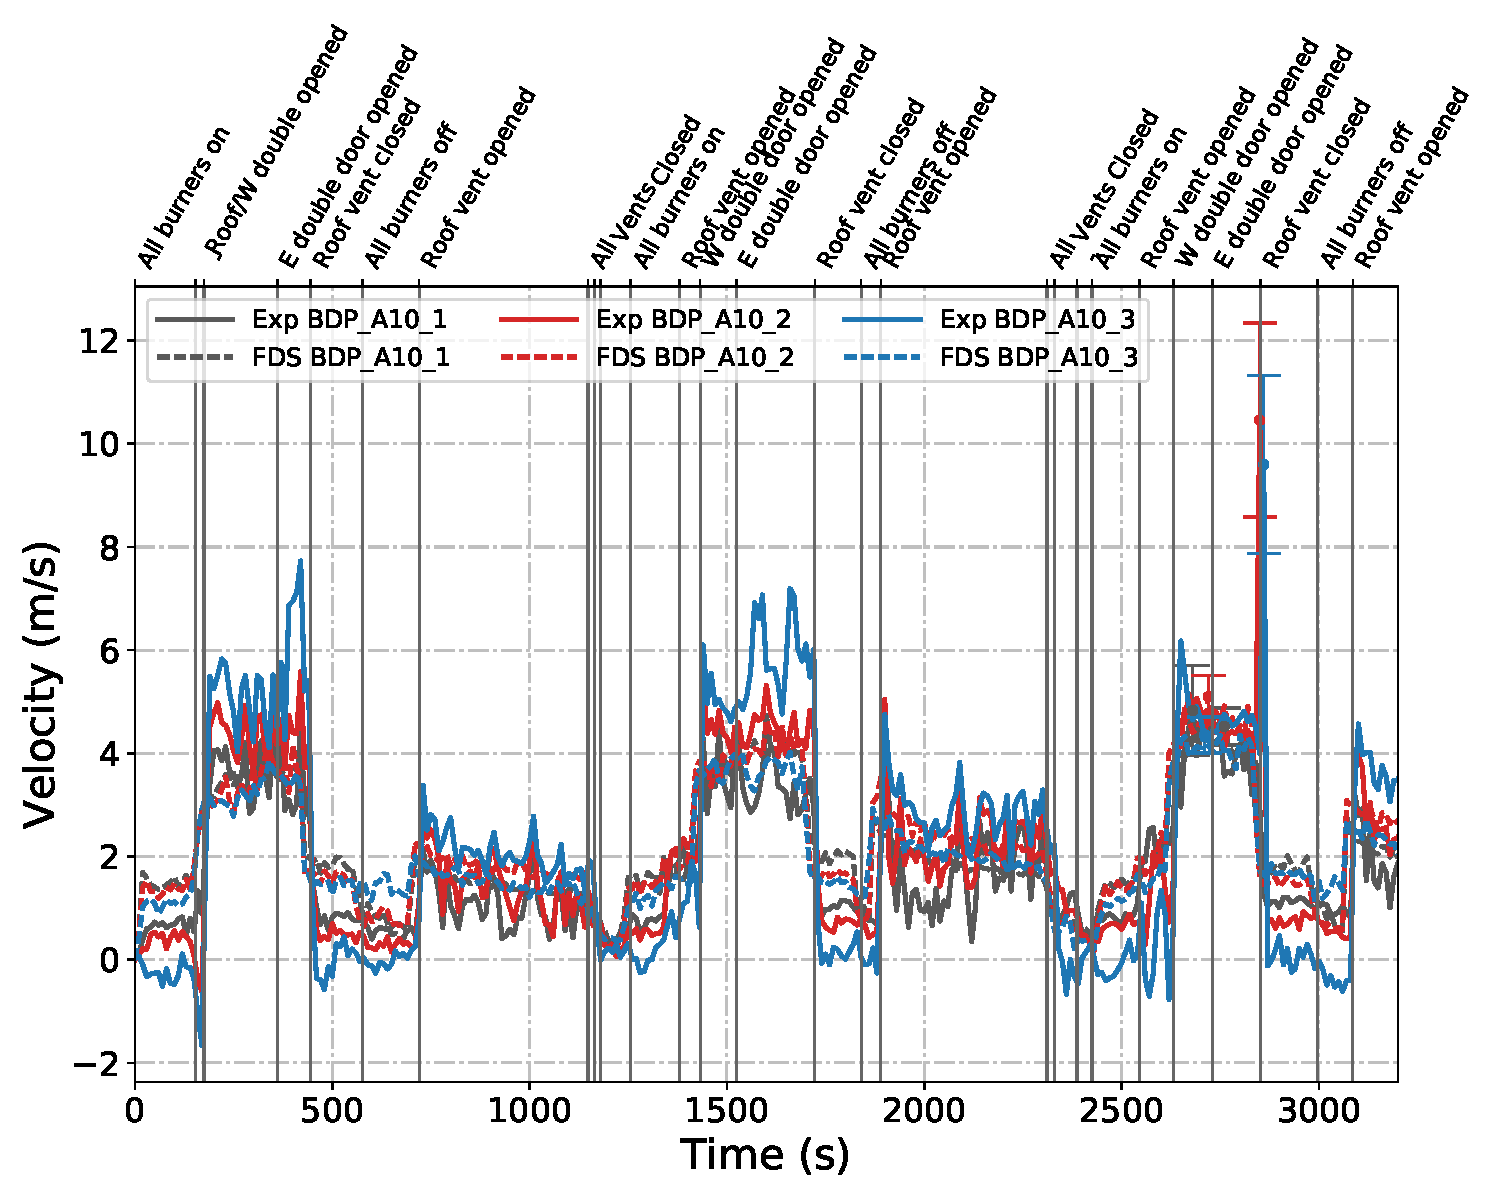
\includegraphics[width=\columnwidth]{Figures/Plots/Validation/Velocity/Test_5_BDP_A10}
	\caption[Plots of measured and predicted gas velocity data at BDP locations in A10 during Test~5.]{Plots of measured and predicted gas velocity data at the BDP locations in array A10 at the East Structure roof vent during Test~5.}
	\label{fig:Test5_BDPs}
\end{figure}

\begin{figure}[!h]
	\centering
	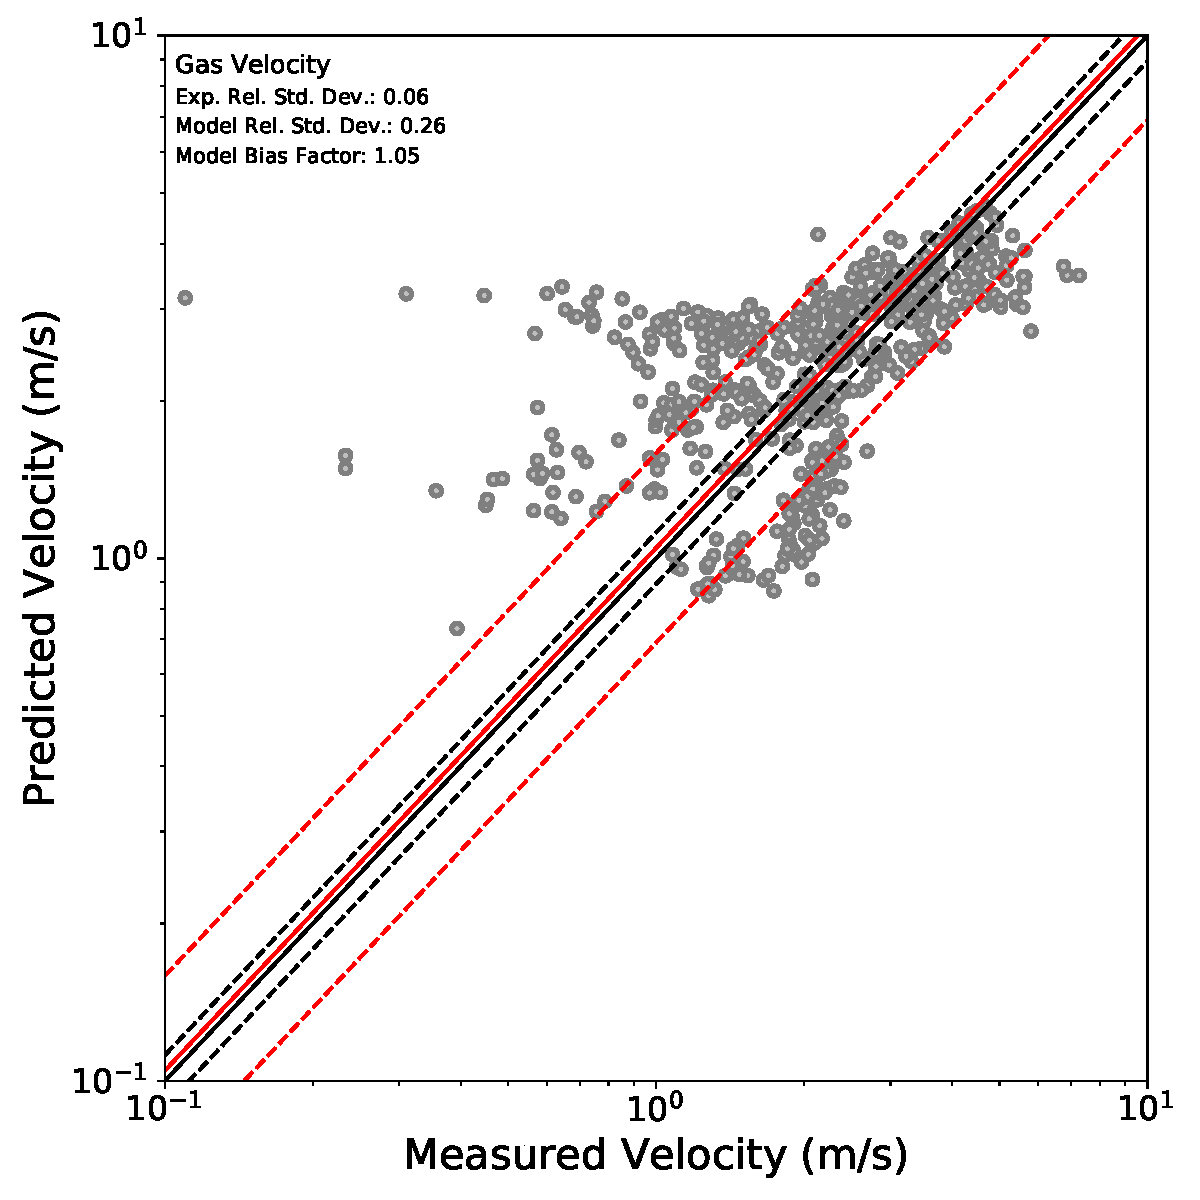
\includegraphics[width=\columnwidth]{Figures/Plots/Validation/Velocity/loglog_BDPs}
	\caption{Summary of measured and predicted gas velocity measurements.}
	\label{fig:loglog_BDPs}
\end{figure}

\clearpage
\subsection{Total Heat Flux}
The heat flux measured by the total heat flux gauges near the stairway door and near the south door on the second floor of the West Structure are plotted with the predicted heat flux data at the same locations over the duration of Test~23 in Figure~\ref{fig:Test23_HFs} below. The log/log scatter plot generated from the predicted heat flux data and measured heat flux data at the various measurement locations corresponding to the applicable time periods during Tests 5--6 and Tests~22--25 is shown in Figure~\ref{fig:loglog_HFs}.  

\begin{figure}[!h]
	\centering
	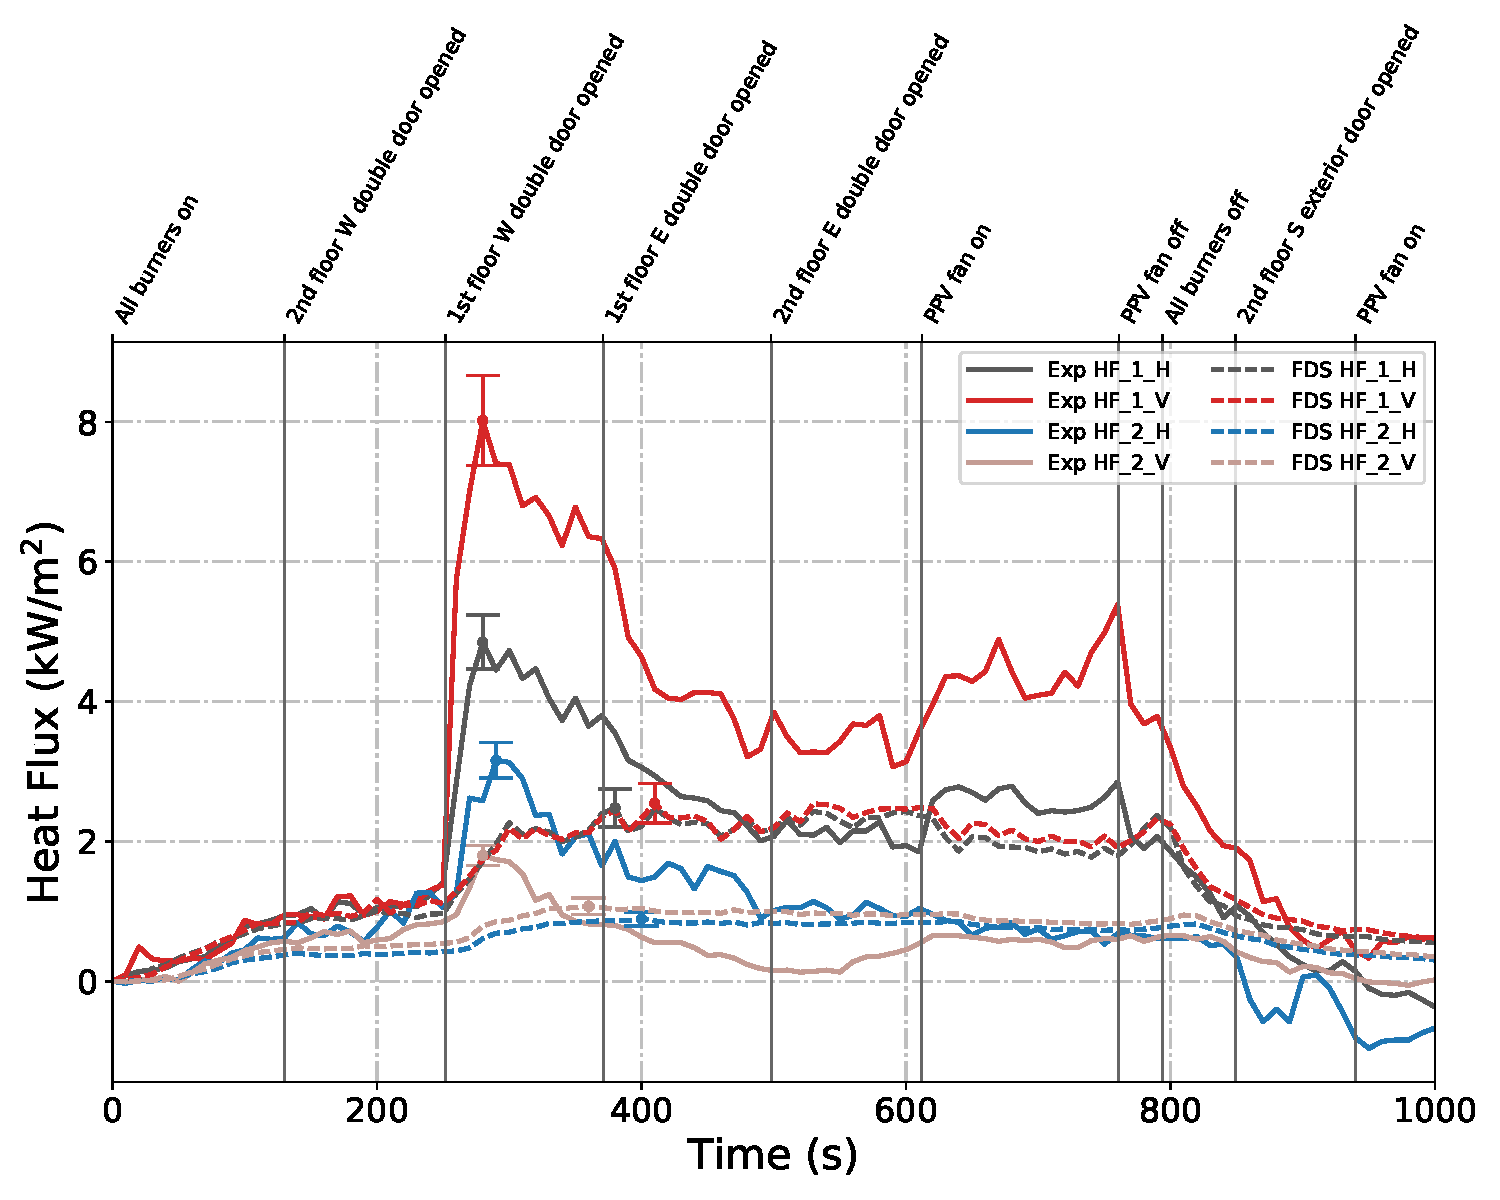
\includegraphics[width=\columnwidth]{Figures/Plots/Validation/Heat_Flux/Test_23_HFs}
	\caption[Plots of measured and predicted heat flux data during Test~23.]{Plots of measured and predicted heat flux data at the locations near the stairway door and near the south door on the second floor of the West Structure during Test~23.}
	\label{fig:Test23_HFs}
\end{figure}

\begin{figure}[!h]
	\centering
	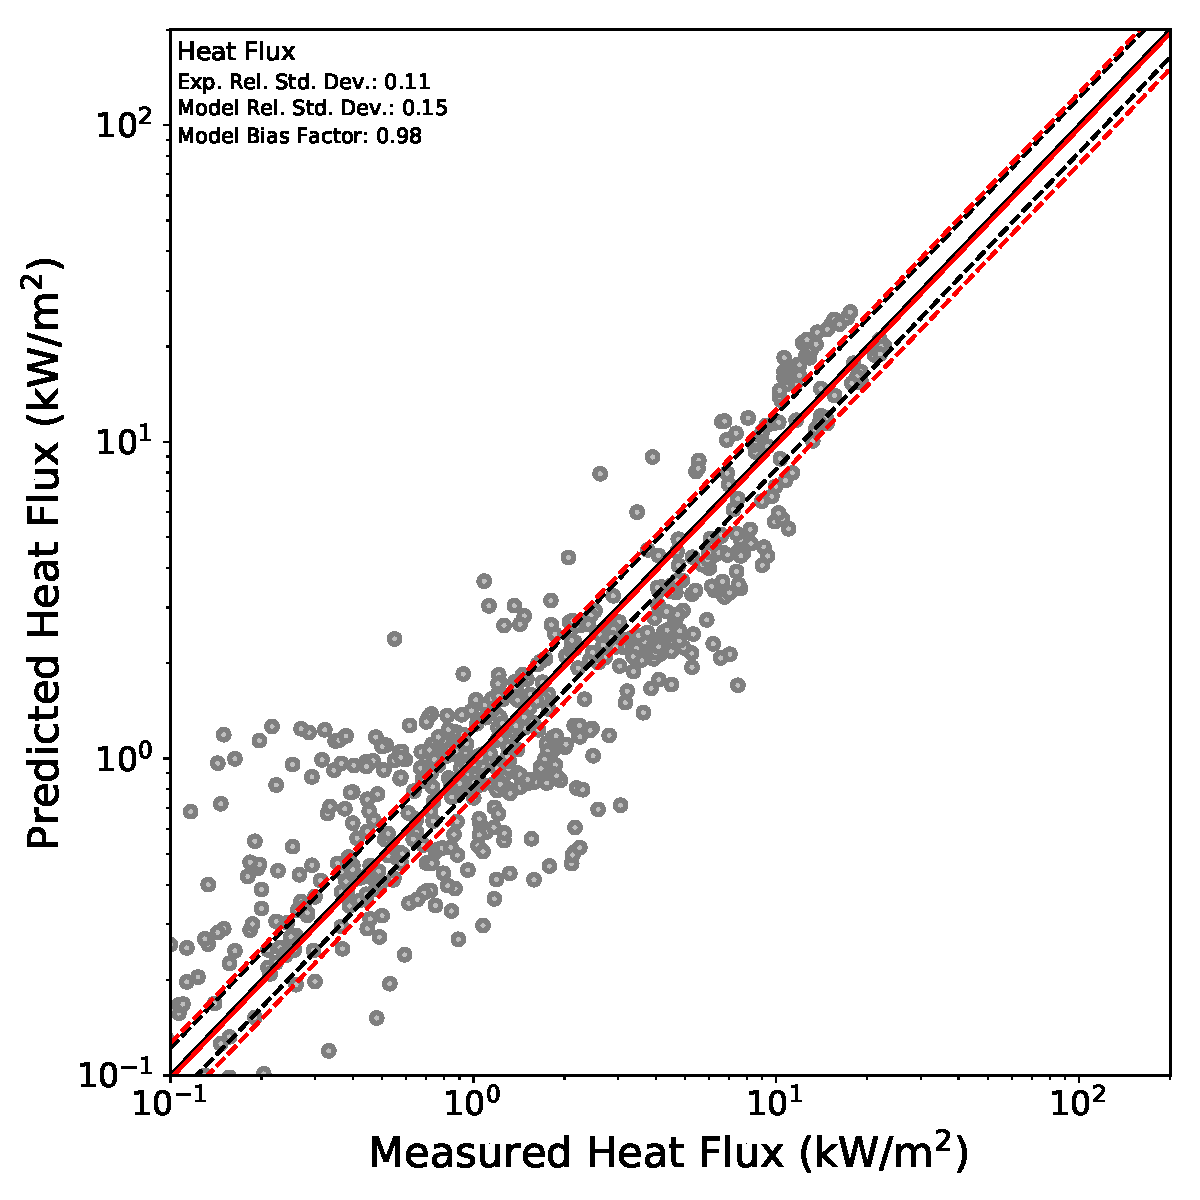
\includegraphics[width=\columnwidth]{Figures/Plots/Validation/Heat_Flux/loglog_HFs}
	\caption{Summary of measured and predicted heat flux measurements.}
	\label{fig:loglog_HFs}
\end{figure}

\clearpage
\subsection{Summary}
Table~\ref{table:stats_compare} compares the model bias factor ($\delta$), the experimental relative standard deviation ($\sigma_E$), and model relative standard deviation ($\sigma_M$) calculated using data from the previously-specified time periods during the six applicable tests for each data quantity discussed above to the values of the same parameters calculated using all the FDS validation data for the same data quantity as stated within the FDS Validation Guide.

\begin{table}[!ht]
\caption[Calculated $\delta$, $\sigma_E$, and $\sigma_M$ Values Compared to the Parameter Values Stated in FDS Validation Guide.]{Model Bias Factor ($\delta$) and Relative Standard Deviation of Experimental Data ($\sigma_E$) and Model Data ($\sigma_M$) Calculated Using the Applicable Predicted and Measured Propane Gas Burner Data Compared to Values of Same Parameters as Provided by the FDS Validation Guide.}
\begin{center}
\begin{tabular}{lcccccccc}
\toprule
					& & \multicolumn{3}{c}{\textbf{\underline{Calculated}}} & & \multicolumn{3}{c}{\textbf{\underline{FDS Validation}}}   \\
\textbf{Quantity} 	& & \multicolumn{3}{c}{\textbf{\underline{Values}}} 	& & \multicolumn{3}{c}{\textbf{\underline{Guide}}} \\
				 	& & $\delta$ 	&  $\sigma_E$ 	& 	$\sigma_M$ 			& & $\delta$ 	&  $\sigma_E$ 	& 	$\sigma_M$ 		\\	
\midrule
Hot Gas Layer 		& & \multirow{2}{*}{0.97} & \multirow{2}{*}{0.05} & \multirow{2}{*}{0.05} & & \multirow{2}{*}{1.04} & \multirow{2}{*}{0.07} & \multirow{2}{*}{0.07} 	\\
Temperature 		& &					   	  & 					  & 					  & &						& 					   &						\\
\multicolumn{9}{c}{} \\
Ceiling Jet 		& & \multirow{2}{*}{1.03} & \multirow{2}{*}{0.06} & \multirow{2}{*}{0.06} & & \multirow{2}{*}{1.04} & \multirow{2}{*}{0.07} & \multirow{2}{*}{0.13} 	\\
Temperature 		& & 					  & 					  & 					  & &						& 					   &						\\
\multicolumn{9}{c}{} \\
Oxygen 				& & \multirow{2}{*}{1.08}  & \multirow{2}{*}{0.08} & \multirow{2}{*}{0.15} & & \multirow{2}{*}{0.99} & \multirow{2}{*}{0.08} & \multirow{2}{*}{0.14} 	\\
Concentration 		& & 					   & 					  & 					   & & 						& 					   &						\\
\multicolumn{9}{c}{} \\
Carbon Dioxide 		& & \multirow{2}{*}{0.96}  & \multirow{2}{*}{0.08} & \multirow{2}{*}{0.14} & & \multirow{2}{*}{1.00} & \multirow{2}{*}{0.08} & \multirow{2}{*}{0.12} 	\\
Concentration 		& & 					   & 					  & 					   & & 						& 					   &						\\
\multicolumn{9}{c}{} \\
Gas Velocity 		& & 1.05  & 0.06 & 0.26 & & 0.99 & 0.08 & 0.09 	\\
\multicolumn{9}{c}{} \\
Heat Flux 			& & 0.98  & 0.11 & 0.15 & & 0.98 & 0.11 & 0.24 	\\
\bottomrule
\end{tabular}
\end{center}
\label{table:stats_compare}
\end{table}
\FloatBarrier

Overall, the agreement between the FDS simulation data and experimental data for the considered gas burner experiments is consistent with the statistical values given by the FDS Validation Guide. For the HGL temperature, ceiling jet temperature, and heat flux, the model bias calculated for the gas burner simulations is equal to or better than (closer to the ideal value of 1) the overall model bias values given by the FDS Validation Guide. Additionally, the relative standard deviations of the experimental data and model data for these three quantities are equal to or less than (better than) the corresponding values for the same data types listed in the validation guide. 

The $\delta$, $\sigma_E$, and $\sigma_M$ values produced by the gas burner model and experimental data for both the $O_2$ and $CO_2$ gas concentrations were very close to the values documented in the FDS Validation Guide. The $\sigma_E$ values are equal in both comparisons and the $\sigma_M$ values are greater in magnitude by only 0.01 and 0.02 compared to the validation guide values for oxygen and carbon dioxide concentration, respectively. Finally, based on the data from gas burner simulations, the oxygen concentration model bias is worse (further from the ideal value of 1) by 7~\% and carbon dioxide concentration model bias is worse by 4~\% compared to the documented values in the FDS Validation Guide.

The most significant difference between the documented values and values from the gas burner models occur in the gas velocity comparison, in which $\sigma_M$ was calculated as being greater than the $\sigma_M$ from the validation guide by a value 0.18. This discrepancy may exist for a few of reasons. First, gas velocity was one of the quantities with the highest uncertainty associated with the experimental measurements. Also, as previously mentioned, the experiments were conducted outdoors, so environmental conditions may have affected the measurements, even though only data from BDPs that were fully inside the structures were considered in an attempt to limit such effect. All the data used to calculate the $\delta$, $\sigma_E$, and $\sigma_M$ values in the validation guide correspond to experiments that were  conducted in an indoor laboratory setting, which could explain the significantly smaller model relative standard deviation. Finally, due to the nature of the fire environment at the time of the measurements, it's possible that turbulent flow was occurring through the vents (especially the roof vent in Tests~5 and 6) at the time of the measurements. CFD models that use Large-Eddy Simulation (LES), the default mode of operation for FDS, tend to be limited more in terms of accurately measuring turbulent flow than compared to measurements during other conditions.

%%%%%%%%%%%%%%%%%%%%%%%%%
% CHAPTER 6: Conclusion %
%%%%%%%%%%%%%%%%%%%%%%%%%

\renewcommand{\thechapter}{6}

\chapter{Conclusion}

Nine full-scale fire tests were conducted in two residential-sized structures. Five of the experiments occurred in a single-story structure with three different rooms, and the other four experiments were performed in a two-story structure with the ground level having an open floor plan and the second level having two rooms and a hallway. The fire source for each experiment was provided by a set of three diffusion flame burners with propane as the fuel. Various doors and vents were opened and closed during each test to change ventilation within the structure. Local measurements of temperature, gas velocity, heat flux, and gas concentrations were collected at various locations throughout the structure during the experiments. 

The dimensions of each structure were carefully measured, and their construction materials were well-defined. The locations of the experimental instrumentation were also measured and the times of different experimental events were recorded. Additionally, the total volume of propane delivered to the burners was measured by a rotary gas meter and was used to calculate the heat release rate of the fire during each test. Using this information as input data, simulations of the experiments were created and executed using the CFD program Fire Dynamics Simulator developed by NIST. The simulation results were compared to the experimental data from the experiments.

The agreement between the FDS simulation data and experimental data for the gas burner experiments is consistent with the statistical values given by the FDS Validation Guide. For the quantities of hot gas layer temperature, ceiling jet temperature, and heat flux, the model bias value was equal to or better than (closer to the ideal value of 1) the overall model bias values given by the FDS Validation Guide. Similarly, the relative standard deviations of the experimental data and model data were equal to or less than (more accurate) the corresponding values for the same data types listed in the validation guide. The model bias and experimental and model relative standard deviations produced for both the $O_2$ and $CO_2$ gas concentrations were very close to or better than the values documented in the FDS Validation Guide. The most significant discrepancy between the documented values and values from the gas burner models was seen in the gas velocity comparison. The difference could be a result of the fact that the tests were conducted outdoors, that the instrumentation used to measure gas velocity had a relatively large uncertainty range, and/or the limitations of LES models like FDS to model turbulent gas flow at a fine resolution.

Overall, the comparison of the simulation data to the experimental data suggests that the accuracy of the FDS models of the gas burner experiments in residential-scale structures is sufficient and comparable to the accuracy of other FDS models of different fire scenarios described in the FDS Validation Guide.


%%
%% This is file `supertabular.sty',
%% generated with the docstrip utility.
%%
%% The original source files were:
%%
%% supertabular.dtx  (with options: `package')
%% Copyright (C) 1989-2004 Johannes Braams. All rights reserved.
%% 
%% This file was generated from file(s) of the supertabular package.
%% -----------------------------------------------------------------
%% 
%% It may be distributed and/or modified under the
%% conditions of the LaTeX Project Public License, either version 1.3
%% of this license or (at your option) any later version.
%% The latest version of this license is in
%%   http://www.latex-project.org/lppl.txt
%% and version 1.3 or later is part of all distributions of LaTeX
%% version 2003/12/01 or later.
%% 
%% This work has the LPPL maintenance status "maintained".
%% 
%% The Current Maintainer of this work is Johannes Braams.
%% 
%% This file may only be distributed together with a copy of the
%% supertabular package. You may however distribute the supertabular package
%% without such generated files.
%% 
%% The list of all files belonging to the supertabular package is
%% given in the file `manifest.txt.
%% 
%% The list of derived (unpacked) files belonging to the distribution
%% and covered by LPPL is defined by the unpacking scripts (with
%% extension .ins) which are part of the distribution.
%% Sourcefile `supertabular.dtx'.
%%
%% Copyright (C) 1988 by Theo Jurriens
%% Copyright (C) 1990-2004 by Johannes Braams texniek at braams.cistron.nl
%%                            Kersengaarde 33
%%                            2723 BP Zoetermeer NL
%%                       all rights reserved.
%%
%%
\NeedsTeXFormat{LaTeX2e}
\ProvidesPackage{supertabular}
              [2004/02/20 v4.1e the supertabular environment]
\newcount\c@tracingst
\DeclareOption{errorshow}{\c@tracingst\z@}
\DeclareOption{pageshow}{\c@tracingst\tw@}
\DeclareOption{debugshow}{\c@tracingst5\relax}
\ProcessOptions
\newif\if@topcaption \@topcaptiontrue
\def\topcaption{\@topcaptiontrue\tablecaption}
\def\bottomcaption{\@topcaptionfalse\tablecaption}
\long\def\tablecaption{%
  \refstepcounter{table}\@dblarg{\@xtablecaption}}
\long\def\@xtablecaption[#1]#2{%
  \long\gdef\@process@tablecaption{\ST@caption{table}[#1]{#2}}}
\global\let\@process@tablecaption\relax
\newif\ifST@star
\newif\ifST@mp
\newdimen\ST@wd
\newskip\ST@rightskip
\newskip\ST@leftskip
\newskip\ST@parfillskip
\long\def\ST@caption#1[#2]#3{\par%
  \addcontentsline{\csname ext@#1\endcsname}{#1}%
                  {\protect\numberline{%
                      \csname the#1\endcsname}{\ignorespaces #2}}
  \begingroup
    \@parboxrestore
    \normalsize
    \if@topcaption \vskip -10\p@ \fi
    \@makecaption{\csname fnum@#1\endcsname}{\ignorespaces #3}\par
    \if@topcaption \vskip 10\p@ \fi
  \endgroup}
\newcommand\tablehead[1]{%
  \gdef\@tablehead{%
  \noalign{%
      \global\let\@savcr=\\
      \global\let\\=\org@tabularcr}%
    #1%
    \noalign{\global\let\\=\@savcr}}}
\tablehead{}
\newcommand\tablefirsthead[1]{\gdef\@table@first@head{#1}}
\newcommand\tabletail[1]{%
  \gdef\@tabletail{%
    \noalign{%
      \global\let\@savcr=\\
      \global\let\\=\org@tabularcr}%
    #1%
    \noalign{\global\let\\=\@savcr}}}
\tabletail{}
\newcommand\tablelasttail[1]{\gdef\@table@last@tail{#1}}
\newcommand\sttraceon{\c@tracingst5\relax}
\newcommand\sttraceoff{\c@tracingst\z@}
\newcommand\ST@trace[2]{%
  \ifnum\c@tracingst>#1\relax
    \GenericWarning
      {(supertabular)\@spaces\@spaces}
      {Package supertabular: #2}%
  \fi
  }
\newdimen\ST@pageleft
\newcommand*\shrinkheight[1]{%
  \noalign{\global\advance\ST@pageleft-#1\relax}}
\newcommand*\setSTheight[1]{%
  \noalign{\global\ST@pageleft=#1\relax}}
\newdimen\ST@headht
\newdimen\ST@tailht
\newdimen\ST@pagesofar
\newdimen\ST@pboxht
\newdimen\ST@lineht
\newdimen\ST@stretchht
\newdimen\ST@prevht
\newdimen\ST@toadd
\newdimen\ST@dimen
\newbox\ST@pbox
\def\ST@tabularcr{%
  {\ifnum0=`}\fi
  \@ifstar{\ST@xtabularcr}{\ST@xtabularcr}}
\def\ST@xtabularcr{%
  \@ifnextchar[%]
    {\ST@argtabularcr}%
    {\ifnum0=`{\fi}\cr\ST@cr}}
\def\ST@argtabularcr[#1]{%
  \ifnum0=`{\fi}%
  \ifdim #1>\z@
    \unskip\ST@xargarraycr{#1}
  \else
    \ST@yargarraycr{#1}%
  \fi}
\def\ST@xargarraycr#1{%
  \@tempdima #1\advance\@tempdima \dp \@arstrutbox
  \vrule \@height\z@ \@depth\@tempdima \@width\z@ \cr
  \noalign{\global\ST@toadd=#1}\ST@cr}
\def\ST@yargarraycr#1{%
  \cr\noalign{\vskip #1\global\ST@toadd=#1}\ST@cr}
\def\ST@startpbox#1{%
  \setbox\ST@pbox\vtop\bgroup\hsize#1\@arrayparboxrestore}
\def\ST@astartpbox#1{%
  \bgroup\hsize#1%
  \setbox\ST@pbox\vtop\bgroup\hsize#1\@arrayparboxrestore}
\def\ST@endpbox{%
  \@finalstrut\@arstrutbox\par\egroup
  \ST@dimen=\ht\ST@pbox
  \advance\ST@dimen by \dp\ST@pbox
  \ifnum\ST@pboxht<\ST@dimen
    \global\ST@pboxht=\ST@dimen
  \fi
  \ST@dimen=\z@
  \box\ST@pbox\hfil}
\def\ST@aendpbox{%
  \@finalstrut\@arstrutbox\par\egroup
  \ST@dimen=\ht\ST@pbox
  \advance\ST@dimen by \dp\ST@pbox
  \ifnum\ST@pboxht<\ST@dimen
    \global\ST@pboxht=\ST@dimen
  \fi
  \ST@dimen=\z@
  \unvbox\ST@pbox\egroup\hfil}
\def\estimate@lineht{%
  \ST@lineht=\arraystretch \baslineskp
  \global\advance\ST@lineht by 1\p@
  \ST@stretchht\ST@lineht\advance\ST@stretchht-\baslineskp
  \ifdim\ST@stretchht<\z@\ST@stretchht\z@\fi
  \ST@trace\tw@{Average line height: \the\ST@lineht}%
  \ST@trace\tw@{Stretched line height: \the\ST@stretchht}%
  }
\def\@calfirstpageht{%
  \ST@trace\tw@{Calculating height of tabular on first page}%
  \global\ST@pagesofar\pagetotal
  \global\ST@pageleft\@colroom
  \ST@trace\tw@{Height of text = \the\pagetotal; \MessageBreak
                Height of page = \the\ST@pageleft}%
  \if@twocolumn
    \ST@trace\tw@{two column mode}%
    \if@firstcolumn
     \ST@trace\tw@{First column}%
      \ifnum\ST@pagesofar > \ST@pageleft
        \global\ST@pageleft=2\ST@pageleft
        \ifnum\ST@pagesofar > \ST@pageleft
          \newpage\@calnextpageht
          \ST@trace\tw@{starting new page}%
        \else
          \ST@trace\tw@{Second column}%
          \global\advance\ST@pageleft -\ST@pagesofar
          \global\advance\ST@pageleft -\@colroom
        \fi
      \else
        \global\advance\ST@pageleft by -\ST@pagesofar
        \global\ST@pagesofar\z@
      \fi
    \else
      \ST@trace\tw@{Second column}
      \ifnum\ST@pagesofar > \ST@pageleft
        \ST@trace\tw@{starting new page}%
        \newpage\@calnextpageht
      \else
        \global\advance\ST@pageleft by -\ST@pagesofar
        \global\ST@pagesofar\z@
      \fi
    \fi
  \else
    \ST@trace\tw@{one column mode}%
    \ifnum\ST@pagesofar > \ST@pageleft
      \ST@trace\tw@{starting new page}%
      \newpage\@calnextpageht
    \else
      \global\advance\ST@pageleft by -\ST@pagesofar
      \global\ST@pagesofar\z@
    \fi
  \fi
  \ST@trace\tw@{Available height: \the\ST@pageleft}%
  \ifx\@@tablehead\@empty
    \ST@headht=\z@
  \else
    \setbox\@tempboxa=\vbox{\@arrayparboxrestore
      \ST@restore
      \expandafter\tabular\expandafter{\ST@tableformat}%
      \@@tablehead\endtabular}%
    \ST@headht=\ht\@tempboxa\advance\ST@headht\dp\@tempboxa
  \fi
  \ST@trace\tw@{Height of head: \the\ST@headht}%
  \ifx\@tabletail\@empty
    \ST@tailht=\z@
  \else
    \setbox\@tempboxa=\vbox{\@arrayparboxrestore
      \ST@restore
      \expandafter\tabular\expandafter{\ST@tableformat}
        \@tabletail\endtabular}
    \ST@tailht=\ht\@tempboxa\advance\ST@tailht\dp\@tempboxa
  \fi
  \advance\ST@tailht by \ST@lineht
  \ST@trace\tw@{Height of tail: \the\ST@tailht}%
  \ST@trace\tw@{Maximum height of tabular: \the\ST@pageleft}%
  \@tempdima\ST@headht
  \advance\@tempdima\ST@lineht
  \advance\@tempdima\ST@tailht
  \ST@trace\tw@{Minimum height of tabular: \the\@tempdima}%
  \ifnum\@tempdima>\ST@pageleft
    \ST@trace\tw@{starting new page}%
    \newpage\@calnextpageht
  \fi
}
\def\@calnextpageht{%
  \ST@trace\tw@{Calculating height of tabular on next page}%
  \global\ST@pageleft\@colroom
  \global\ST@pagesofar=\z@
  \ST@trace\tw@{Maximum height of tabular: \the\ST@pageleft}%
  }
\def\x@supertabular{%
  \let\org@tabular\tabular
  \let\tabular\inner@tabular
  \expandafter\let
    \csname org@tabular*\expandafter\endcsname
    \csname tabular*\endcsname
  \expandafter\let\csname tabular*\expandafter\endcsname
    \csname inner@tabular*\endcsname
  \if@topcaption \@process@tablecaption \fi
  \global\let\@oldcr=\\
  \def\baslineskp{\baselineskip}%
  \ifx\undefined\@classix
    \let\org@tabularcr\@tabularcr
    \let\@tabularcr\ST@tabularcr
    \let\org@startpbox=\@startpbox
    \let\org@endpbox=\@endpbox
    \let\@@startpbox=\ST@startpbox
    \let\@@endpbox=\ST@endpbox
  \else
    \let\org@tabularcr\@arraycr
    \let\@arraycr\ST@tabularcr
    \let\org@startpbox=\@startpbox
    \let\org@endpbox=\@endpbox
    \let\@startpbox=\ST@astartpbox
    \let\@endpbox=\ST@aendpbox
  \fi
  \ifx\@table@first@head\undefined
    \let\@@tablehead=\@tablehead
  \else
    \let\@@tablehead=\@table@first@head
  \fi
  \let\ST@skippage\ST@skipfirstpart
  \estimate@lineht
  \@calfirstpageht
  \noindent
  }
\def\supertabular{%
  \@ifnextchar[{\@supertabular}%]
               {\@supertabular[]}}
\def\@supertabular[#1]#2{%
  \def\ST@tableformat{#2}%
  \ST@trace\tw@{Starting a new supertabular}%
  \global\ST@starfalse
  \global\ST@mpfalse
  \x@supertabular
  \expandafter\org@tabular\expandafter{\ST@tableformat}%
  \@@tablehead}
\@namedef{supertabular*}#1{%
  \@ifnextchar[{\@nameuse{@supertabular*}{#1}}%
               {\@nameuse{@supertabular*}{#1}[]}%]
  }
\@namedef{@supertabular*}#1[#2]#3{%
  \ST@trace\tw@{Starting a new supertabular*}%
  \def\ST@tableformat{#3}%
  \ST@wd=#1\relax
  \global\ST@startrue
  \global\ST@mpfalse
  \x@supertabular
  \expandafter\csname org@tabular*\expandafter\endcsname
  \expandafter{\expandafter\ST@wd\expandafter}%
  \expandafter{\ST@tableformat}%
  \@@tablehead}%
\def\mpsupertabular{%
  \@ifnextchar[{\@mpsupertabular}%]
               {\@mpsupertabular[]}}
\def\@mpsupertabular[#1]#2{%
  \def\ST@tableformat{#2}%
  \ST@trace\tw@{Starting a new mpsupertabular}%
  \global\ST@starfalse
  \global\ST@mptrue
  \ST@rightskip \rightskip
  \ST@leftskip \leftskip
  \ST@parfillskip \parfillskip
  \x@supertabular
  \minipage{\columnwidth}%
  \parfillskip\ST@parfillskip
  \rightskip \ST@rightskip
  \leftskip \ST@leftskip
  \noindent\expandafter\org@tabular\expandafter{\ST@tableformat}%
  \@@tablehead}
\@namedef{mpsupertabular*}#1{%
  \@ifnextchar[{\@nameuse{@mpsupertabular*}{#1}}%
               {\@nameuse{@mpsupertabular*}{#1}[]}%]
  }
\@namedef{@mpsupertabular*}#1[#2]#3{%
  \ST@trace\tw@{Starting a new mpsupertabular*}%
  \def\ST@tableformat{#3}%
  \ST@wd=#1\relax
  \global\ST@startrue
  \global\ST@mptrue
  \ST@rightskip \rightskip
  \ST@leftskip \leftskip
  \ST@parfillskip \parfillskip
  \x@supertabular
  \minipage{\columnwidth}%
  \parfillskip\ST@parfillskip
  \rightskip \ST@rightskip
  \leftskip \ST@leftskip
  \noindent\expandafter\csname org@tabular*\expandafter\endcsname
  \expandafter{\expandafter\ST@wd\expandafter}%
  \expandafter{\ST@tableformat}%
  \@@tablehead}%
\def\endsupertabular{%
  \ifx\@table@last@tail\undefined
    \@tabletail
  \else
    \@table@last@tail
  \fi
  \csname endtabular\ifST@star*\fi\endcsname
  \ST@restore
  \if@topcaption
  \else
    \@process@tablecaption
    \@topcaptiontrue
  \fi
  \global\let\\\@oldcr
  \global\let\@process@tablecaption\relax
  \ST@trace\tw@{Ended a supertabular\ifST@star*\fi}%
  }
\expandafter\let\csname endsupertabular*\endcsname\endsupertabular
\def\endmpsupertabular{%
  \ifx\@table@last@tail\undefined
    \@tabletail
  \else
    \@table@last@tail
  \fi
  \csname endtabular\ifST@star*\fi\endcsname
  \endminipage
  \ST@restore
  \if@topcaption
  \else
    \@process@tablecaption
    \@topcaptiontrue
  \fi
  \global\let\\\@oldcr
  \global\let\@process@tablecaption\relax
  \ST@trace\tw@{Ended a mpsupertabular\ifST@star*\fi}%
  }
\expandafter\let\csname endmpsupertabular*\endcsname\endmpsupertabular
\def\ST@restore{%
  \ifx\undefined\@classix
    \let\@tabularcr\org@tabularcr
  \else
    \let\@arraycr\org@tabularcr
  \fi
  \let\@startpbox\org@startpbox
  \let\@endpbox\org@endpbox
  }
\def\inner@tabular{%
  \ST@restore
  \let\\\@oldcr
  \noindent
  \org@tabular}
\@namedef{inner@tabular*}{%
  \ST@restore
  \let\\\@oldcr
  \noindent
  \csname org@tabular*\endcsname}
\def\ST@cr{%
  \noalign{%
    \ifnum\ST@pboxht<\ST@lineht
      \global\advance\ST@pageleft -\ST@lineht
      \global\ST@prevht\ST@lineht
    \else
     \ST@trace\thr@@{Added par box with height \the\ST@pboxht}%
      \global\advance\ST@pageleft -\ST@pboxht
      \global\advance\ST@pageleft -0.1\ST@pboxht
      \global\advance\ST@pageleft -\ST@stretchht
      \global\ST@prevht\ST@pboxht
      \global\ST@pboxht\z@
    \fi
    \global\advance\ST@pageleft -\ST@toadd
    \global\ST@toadd=\z@
    \ST@trace\thr@@{Space left for tabular: \the\ST@pageleft}%
  }
  \noalign{\global\let\ST@next\@empty}%
  \ifnum\ST@pageleft<\z@
    \ST@skippage
  \else
    \noalign{\global\@tempdima\ST@tailht
      \global\advance\@tempdima\ST@prevht
    \ifST@mp
      \ifvoid\@mpfootins\else
        \global\advance\@tempdima\ht\@mpfootins
        \global\advance\@tempdima 3pt
      \fi
    \fi}
    \ifnum\ST@pageleft<\@tempdima
      \ST@newpage
    \fi
  \fi
  \ST@next}
\def\ST@skipfirstpart{%
  \noalign{%
    \ST@trace\tw@{Tabular too high, moving to next page}%
    \global\advance\ST@pageleft\pagetotal
    \global\ST@pagesofar\z@
    \newpage
    \global\let\ST@skippage\ST@newpage
    }}
\def\ST@newpage{%
  \noalign{\ST@trace\tw@{Starting new page, writing tail}}%
  \@tabletail
  \ifST@star
    \csname endtabular*\endcsname
  \else
    \endtabular
  \fi
  \ifST@mp
    \endminipage
  \fi
  \global\let\ST@skippage\ST@newpage
  \newpage\@calnextpageht
  \let\ST@next\@tablehead
  \ST@trace\tw@{writing head}%
  \ifST@mp
    \noindent\minipage{\columnwidth}%
    \parfillskip\ST@parfillskip
    \rightskip \ST@rightskip
    \leftskip \ST@leftskip
  \fi
  \noindent
  \ifST@star
    \expandafter\csname org@tabular*\expandafter\endcsname
    \expandafter{\expandafter\ST@wd\expandafter}%
    \expandafter{\ST@tableformat}%
  \else
    \expandafter\org@tabular\expandafter{\ST@tableformat}%
  \fi}
\endinput
%%
%% End of file `supertabular.sty'.

\titleformat{\chapter}
      {\normalfont\large}{Appendix \thechapter:}{1em}{}
\appendix
\renewcommand{\thechapter}{A}
\renewcommand{\chaptername}{Appendix}

\chapter{Channel Lists}
\label{chap:channel_lists}

\section{East Structure}

\renewcommand{\baselinestretch}{1}
\small\normalsize
\begin{longtable}[c]{c|lll}
\caption[East Structure Channel List]{East Structure Channel List}
\label{table:east_channel_list}\\
\toprule
\begin{tabular}{c} \textbf{Device} \\ \textbf{Location} \end{tabular} &
\begin{tabular}{c} \textbf{Channel} \\ \textbf{Name} \end{tabular}  &
\textbf{Channel Location} &
\textbf{Measurement Type} \\
\midrule
\endfirsthead
\caption[]{East Structure Channel List (continued)} \\
\toprule
\begin{tabular}{c} \textbf{Device} \\ \textbf{Location} \end{tabular} &
\begin{tabular}{c} \textbf{Channel} \\ \textbf{Name} \end{tabular}  &
\textbf{Channel Location} &
\textbf{Measurement Type} \\
\midrule
\endhead
\multirow{13}{*}{\large\textbf{A1}}
 & TC\_A1\_1  & 0.03~m below ceiling & Temperature \\
 & TC\_A1\_2  & 0.30~m below ceiling & Temperature \\
 & TC\_A1\_3  & 0.61~m below ceiling & Temperature \\
 & TC\_A1\_4  & 0.91~m below ceiling & Temperature \\
 & TC\_A1\_5  & 1.22~m below ceiling & Temperature \\
 & TC\_A1\_6  & 1.52~m below ceiling & Temperature \\
 & TC\_A1\_7  & 1.83~m below ceiling & Temperature \\
 & TC\_A1\_8  & 2.13~m below ceiling & Temperature \\
\cline{2-4}
 & HF\_A1	  & 0.15~m above floor   & Total heat flux \\
 & RAD\_A1    & 0.15~m above floor   & Radiative heat flux \\
\cline{2-4}
 & CO\_A      & 1.22~m above floor   & CO concentration \\
 & CO2\_A     & 1.22~m above floor   & CO$_2$ concentration \\
 & O2\_A      & 1.22~m above floor   & O$_2$ concentration \\
\midrule
\multirow{10}{*}{\large{\textbf{A2}}}
 & TC\_A2\_1  & 0.03~m below ceiling & Temperature \\
 & TC\_A2\_2  & 0.30~m below ceiling & Temperature \\
 & TC\_A2\_3  & 0.61~m below ceiling & Temperature \\
 & TC\_A2\_4  & 0.91~m below ceiling & Temperature \\
 & TC\_A2\_5  & 1.22~m below ceiling & Temperature \\
 & TC\_A2\_6  & 1.52~m below ceiling & Temperature \\
 & TC\_A2\_7  & 1.83~m below ceiling & Temperature \\
 & TC\_A2\_8  & 2.13~m below ceiling & Temperature \\
\cline{2-4}
 & HF\_A2	  & 0.15~m above floor   & Total heat flux \\
 & RAD\_A2    & 0.15~m above floor   & Radiative heat flux \\
\bottomrule
\newpage
 \multirow{10}{*}{\large{\textbf{A3}}}
 & TC\_A3\_1  & 0.03~m below ceiling & Temperature \\
 & TC\_A3\_2  & 0.30~m below ceiling & Temperature \\
 & TC\_A3\_3  & 0.61~m below ceiling & Temperature \\
 & TC\_A3\_4  & 0.91~m below ceiling & Temperature \\
 & TC\_A3\_5  & 1.22~m below ceiling & Temperature \\
 & TC\_A3\_6  & 1.52~m below ceiling & Temperature \\
 & TC\_A3\_7  & 1.83~m below ceiling & Temperature \\
 & TC\_A3\_8  & 2.13~m below ceiling & Temperature \\
\cline{2-4}
 & HF\_A3	  & 0.15~m above floor   & Total heat flux \\
 & RAD\_A3    & 0.15~m above floor   & Radiative heat flux \\
\midrule
\multirow{13}{*}{\large\textbf{A4}}
 & TC\_A4\_1  & 0.03~m below ceiling & Temperature \\
 & TC\_A4\_2  & 0.30~m below ceiling & Temperature \\
 & TC\_A4\_3  & 0.61~m below ceiling & Temperature \\
 & TC\_A4\_4  & 0.91~m below ceiling & Temperature \\
 & TC\_A4\_5  & 1.22~m below ceiling & Temperature \\
 & TC\_A4\_6  & 1.52~m below ceiling & Temperature \\
 & TC\_A4\_7  & 1.83~m below ceiling & Temperature \\
 & TC\_A4\_8  & 2.13~m below ceiling & Temperature \\
\cline{2-4}
 & HF\_A4	  & 0.15~m above floor   & Total heat flux \\
 & RAD\_A4    & 0.15~m above floor   & Radiative heat flux \\
\cline{2-4}
 & CO\_B      & 1.22~m above floor   & CO concentration \\
 & CO2\_B     & 1.22~m above floor   & CO$_2$ concentration \\
 & O2\_B      & 1.22~m above floor   & O$_2$ concentration \\
\midrule
\multirow{10}{*}{\large{\textbf{A5}}}
 & TC\_A5\_1  & 0.03~m below ceiling & Temperature \\
 & TC\_A5\_2  & 0.30~m below ceiling & Temperature \\
 & TC\_A5\_3  & 0.61~m below ceiling & Temperature \\
 & TC\_A5\_4  & 0.91~m below ceiling & Temperature \\
 & TC\_A5\_5  & 1.22~m below ceiling & Temperature \\
 & TC\_A5\_6  & 1.52~m below ceiling & Temperature \\
 & TC\_A5\_7  & 1.83~m below ceiling & Temperature \\
 & TC\_A5\_8  & 2.13~m below ceiling & Temperature \\
\cline{2-4}
 & HF\_A5	  & 0.15~m above floor   & Total heat flux \\
 & RAD\_A5    & 0.15~m above floor   & Radiative heat flux \\
\bottomrule
\newpage
\multirow{16}{*}{\large{\textbf{A7}}}
 & TC\_A7\_1  & 0.08~m below soffit  & Temperature \\
 & TC\_A7\_2  & 0.34~m below soffit  & Temperature \\
 & TC\_A7\_3  & 0.61~m below soffit  & Temperature \\
 & TC\_A7\_4  & 0.88~m below soffit  & Temperature \\
 & TC\_A7\_5  & 1.15~m below soffit  & Temperature \\
 & TC\_A7\_6  & 1.42~m below soffit  & Temperature \\
 & TC\_A7\_7  & 1.68~m below soffit  & Temperature \\
 & TC\_A7\_8  & 1.95~m below soffit  & Temperature \\
\cline{2-4}
 & BDP\_A7\_1 & 0.08~m below soffit  & Velocity \\
 & BDP\_A7\_2 & 0.34~m below soffit  & Velocity \\
 & BDP\_A7\_3 & 0.61~m below soffit  & Velocity \\
 & BDP\_A7\_4 & 0.88~m below soffit  & Velocity \\
 & BDP\_A7\_5 & 1.15~m below soffit  & Velocity \\
 & BDP\_A7\_6 & 1.42~m below soffit  & Velocity \\
 & BDP\_A7\_7 & 1.68~m below soffit  & Velocity \\
 & BDP\_A7\_8 & 1.95~m below soffit  & Velocity \\
\midrule
\multirow{16}{*}{\large{\textbf{A8}}}
 & TC\_A8\_1  & 0.08~m below soffit  & Temperature \\
 & TC\_A8\_2  & 0.34~m below soffit  & Temperature \\
 & TC\_A8\_3  & 0.61~m below soffit  & Temperature \\
 & TC\_A8\_4  & 0.88~m below soffit  & Temperature \\
 & TC\_A8\_5  & 1.15~m below soffit  & Temperature \\
 & TC\_A8\_6  & 1.42~m below soffit  & Temperature \\
 & TC\_A8\_7  & 1.68~m below soffit  & Temperature \\
 & TC\_A8\_8  & 1.95~m below soffit  & Temperature \\
\cline{2-4}
 & BDP\_A8\_1 & 0.08~m below soffit  & Velocity \\
 & BDP\_A8\_2 & 0.34~m below soffit  & Velocity \\
 & BDP\_A8\_3 & 0.61~m below soffit  & Velocity \\
 & BDP\_A8\_4 & 0.88~m below soffit  & Velocity \\
 & BDP\_A8\_5 & 1.15~m below soffit  & Velocity \\
 & BDP\_A8\_6 & 1.42~m below soffit  & Velocity \\
 & BDP\_A8\_7 & 1.68~m below soffit  & Velocity \\
 & BDP\_A8\_8 & 1.95~m below soffit  & Velocity \\
\bottomrule
\newpage
\multirow{16}{*}{\large{\textbf{A9}}}
 & TC\_A9\_1  & 0.08~m below soffit  & Temperature \\
 & TC\_A9\_2  & 0.34~m below soffit  & Temperature \\
 & TC\_A9\_3  & 0.61~m below soffit  & Temperature \\
 & TC\_A9\_4  & 0.88~m below soffit  & Temperature \\
 & TC\_A9\_5  & 1.15~m below soffit  & Temperature \\
 & TC\_A9\_6  & 1.42~m below soffit  & Temperature \\
 & TC\_A9\_7  & 1.68~m below soffit  & Temperature \\
 & TC\_A9\_8  & 1.95~m below soffit  & Temperature \\
\cline{2-4}
 & BDP\_A9\_1 & 0.08~m below soffit  & Velocity \\
 & BDP\_A9\_2 & 0.34~m below soffit  & Velocity \\
 & BDP\_A9\_3 & 0.61~m below soffit  & Velocity \\
 & BDP\_A9\_4 & 0.88~m below soffit  & Velocity \\
 & BDP\_A9\_5 & 1.15~m below soffit  & Velocity \\
 & BDP\_A9\_6 & 1.42~m below soffit  & Velocity \\
 & BDP\_A9\_7 & 1.68~m below soffit  & Velocity \\
 & BDP\_A9\_8 & 1.95~m below soffit  & Velocity \\
\midrule
\multirow{6}{*}{\large{\textbf{A10}}}
 & TC\_A10\_1 & 0.91~m from S side of vent & Temperature \\
 & TC\_A10\_2 & 0.61~m from S side of vent & Temperature \\
 & TC\_A10\_3 & 0.30~m from S side of vent & Temperature \\
\cline{2-4}
 & BDP\_A10\_1 & 0.91~m from S side of vent & Velocity \\
 & BDP\_A10\_2 & 0.61~m from S side of vent & Velocity \\
 & BDP\_A10\_3 & 0.30~m from S side of vent & Velocity \\
\bottomrule
\end{longtable}
\clearpage
\renewcommand{\baselinestretch}{2}
\small\normalsize

\section{West Structure}

\renewcommand{\baselinestretch}{1}
\small\normalsize
\begin{longtable}[c]{c|lll}
\caption[West Structure Channel List]{West Structure Channel List}
\label{table:west_channel_list}\\
\toprule
\begin{tabular}{c} \textbf{Device} \\ \textbf{Location} \end{tabular} &
\begin{tabular}{c} \textbf{Channel} \\ \textbf{Name} \end{tabular}  &
\textbf{Channel Location} &
\textbf{Measurement Type} \\
\midrule
\endfirsthead
\caption[]{West Structure Channel List (continued)} \\
\toprule
\begin{tabular}{c} \textbf{Device} \\ \textbf{Location} \end{tabular} &
\begin{tabular}{c} \textbf{Channel} \\ \textbf{Name} \end{tabular}  &
\textbf{Channel Location} &
\textbf{Measurement Type} \\
\midrule
\endhead
\multirow{11}{*}{\large\textbf{A1}}
 & TC\_A1\_1  & 0.03~m below ceiling & Temperature \\
 & TC\_A1\_2  & 0.30~m below ceiling & Temperature \\
 & TC\_A1\_3  & 0.61~m below ceiling & Temperature \\
 & TC\_A1\_4  & 0.91~m below ceiling & Temperature \\
 & TC\_A1\_5  & 1.22~m below ceiling & Temperature \\
 & TC\_A1\_6  & 1.52~m below ceiling & Temperature \\
 & TC\_A1\_7  & 1.83~m below ceiling & Temperature \\
 & TC\_A1\_8  & 2.13~m below ceiling & Temperature \\
\cline{2-4}
 & CO\_A      & 1.22~m above floor   & CO concentration \\
 & CO2\_A     & 1.22~m above floor   & CO$_2$ concentration \\
 & O2\_A      & 1.22~m above floor   & O$_2$ concentration \\
\midrule
\multirow{10}{*}{\large{\textbf{A2}}}
 & TC\_A2\_1  & 0.03~m below ceiling & Temperature \\
 & TC\_A2\_2  & 0.30~m below ceiling & Temperature \\
 & TC\_A2\_3  & 0.61~m below ceiling & Temperature \\
 & TC\_A2\_4  & 0.91~m below ceiling & Temperature \\
 & TC\_A2\_5  & 1.22~m below ceiling & Temperature \\
 & TC\_A2\_6  & 1.52~m below ceiling & Temperature \\
 & TC\_A2\_7  & 1.83~m below ceiling & Temperature \\
 & TC\_A2\_8  & 2.13~m below ceiling & Temperature \\
\midrule
 \multirow{10}{*}{\large{\textbf{A3}}}
 & TC\_A3\_1  & 0.03~m below ceiling & Temperature \\
 & TC\_A3\_2  & 0.30~m below ceiling & Temperature \\
 & TC\_A3\_3  & 0.61~m below ceiling & Temperature \\
 & TC\_A3\_4  & 0.91~m below ceiling & Temperature \\
 & TC\_A3\_5  & 1.22~m below ceiling & Temperature \\
 & TC\_A3\_6  & 1.52~m below ceiling & Temperature \\
 & TC\_A3\_7  & 1.83~m below ceiling & Temperature \\
 & TC\_A3\_8  & 2.13~m below ceiling & Temperature \\
\bottomrule
\newpage
\multirow{16}{*}{\large{\textbf{A5}}}
 & TC\_A5\_1  & 0.08~m below soffit  & Temperature \\
 & TC\_A5\_2  & 0.34~m below soffit  & Temperature \\
 & TC\_A5\_3  & 0.61~m below soffit  & Temperature \\
 & TC\_A5\_4  & 0.88~m below soffit  & Temperature \\
 & TC\_A5\_5  & 1.15~m below soffit  & Temperature \\
 & TC\_A5\_6  & 1.42~m below soffit  & Temperature \\
 & TC\_A5\_7  & 1.68~m below soffit  & Temperature \\
 & TC\_A5\_8  & 1.95~m below soffit  & Temperature \\
\cline{2-4}
 & BDP\_A5\_1 & 0.08~m below soffit  & Velocity \\
 & BDP\_A5\_2 & 0.34~m below soffit  & Velocity \\
 & BDP\_A5\_3 & 0.61~m below soffit  & Velocity \\
 & BDP\_A5\_4 & 0.88~m below soffit  & Velocity \\
 & BDP\_A5\_5 & 1.15~m below soffit  & Velocity \\
 & BDP\_A5\_6 & 1.42~m below soffit  & Velocity \\
 & BDP\_A5\_7 & 1.68~m below soffit  & Velocity \\
 & BDP\_A5\_8 & 1.95~m below soffit  & Velocity \\
\midrule
\multirow{16}{*}{\large{\textbf{A6}}}
 & TC\_A6\_1  & 0.08~m below soffit  & Temperature \\
 & TC\_A6\_2  & 0.34~m below soffit  & Temperature \\
 & TC\_A6\_3  & 0.61~m below soffit  & Temperature \\
 & TC\_A6\_4  & 0.88~m below soffit  & Temperature \\
 & TC\_A6\_5  & 1.15~m below soffit  & Temperature \\
 & TC\_A6\_6  & 1.42~m below soffit  & Temperature \\
 & TC\_A6\_7  & 1.68~m below soffit  & Temperature \\
 & TC\_A6\_8  & 1.95~m below soffit  & Temperature \\
\cline{2-4}
 & BDP\_A6\_1 & 0.08~m below soffit  & Velocity \\
 & BDP\_A6\_2 & 0.34~m below soffit  & Velocity \\
 & BDP\_A6\_3 & 0.61~m below soffit  & Velocity \\
 & BDP\_A6\_4 & 0.88~m below soffit  & Velocity \\
 & BDP\_A6\_5 & 1.15~m below soffit  & Velocity \\
 & BDP\_A6\_6 & 1.42~m below soffit  & Velocity \\
 & BDP\_A6\_7 & 1.68~m below soffit  & Velocity \\
 & BDP\_A6\_8 & 1.95~m below soffit  & Velocity \\
\bottomrule
\newpage
\multirow{8}{*}{\large{\textbf{A7}}}
 & TC\_A7\_1  & 0.03~m below ceiling & Temperature \\
 & TC\_A7\_2  & 0.30~m below ceiling & Temperature \\
 & TC\_A7\_3  & 0.61~m below ceiling & Temperature \\
 & TC\_A7\_4  & 0.91~m below ceiling & Temperature \\
 & TC\_A7\_5  & 1.22~m below ceiling & Temperature \\
 & TC\_A7\_6  & 1.52~m below ceiling & Temperature \\
 & TC\_A7\_7  & 1.83~m below ceiling & Temperature \\
 & TC\_A7\_8  & 2.13~m below ceiling & Temperature \\
\midrule
\multirow{8}{*}{\large{\textbf{A8}}}
 & TC\_A8\_1  & 0.03~m below ceiling & Temperature \\
 & TC\_A8\_2  & 0.30~m below ceiling & Temperature \\
 & TC\_A8\_3  & 0.61~m below ceiling & Temperature \\
 & TC\_A8\_4  & 0.91~m below ceiling & Temperature \\
 & TC\_A8\_5  & 1.22~m below ceiling & Temperature \\
 & TC\_A8\_6  & 1.52~m below ceiling & Temperature \\
 & TC\_A8\_7  & 1.83~m below ceiling & Temperature \\
 & TC\_A8\_8  & 2.13~m below ceiling & Temperature \\
\midrule
\multirow{8}{*}{\large{\textbf{A9}}}
 & TC\_A9\_1  & 0.03~m below ceiling & Temperature \\
 & TC\_A9\_2  & 0.30~m below ceiling & Temperature \\
 & TC\_A9\_3  & 0.61~m below ceiling & Temperature \\
 & TC\_A9\_4  & 0.91~m below ceiling & Temperature \\
 & TC\_A9\_5  & 1.22~m below ceiling & Temperature \\
 & TC\_A9\_6  & 1.52~m below ceiling & Temperature \\
 & TC\_A9\_7  & 1.83~m below ceiling & Temperature \\
 & TC\_A9\_8  & 2.13~m below ceiling & Temperature \\
\bottomrule
\newpage
\multirow{19}{*}{\large\textbf{A10}}
 & TC\_A10\_1  & 0.08~m below soffit  & Temperature \\
 & TC\_A10\_2  & 0.34~m below soffit  & Temperature \\
 & TC\_A10\_3  & 0.61~m below soffit  & Temperature \\
 & TC\_A10\_4  & 0.88~m below soffit  & Temperature \\
 & TC\_A10\_5  & 1.15~m below soffit  & Temperature \\
 & TC\_A10\_6  & 1.42~m below soffit  & Temperature \\
 & TC\_A10\_7  & 1.68~m below soffit  & Temperature \\
 & TC\_A10\_8  & 1.95~m below soffit  & Temperature \\
\cline{2-4}
 & BDP\_A10\_1 & 0.08~m below soffit  & Velocity \\
 & BDP\_A10\_2 & 0.34~m below soffit  & Velocity \\
 & BDP\_A10\_3 & 0.61~m below soffit  & Velocity \\
 & BDP\_A10\_4 & 0.88~m below soffit  & Velocity \\
 & BDP\_A10\_5 & 1.15~m below soffit  & Velocity \\
 & BDP\_A10\_6 & 1.42~m below soffit  & Velocity \\
 & BDP\_A10\_7 & 1.68~m below soffit  & Velocity \\
 & BDP\_A10\_8 & 1.95~m below soffit  & Velocity \\
\cline{2-4}
 & CO\_B      & 1.22~m above floor   & CO concentration \\
 & CO2\_B     & 1.22~m above floor   & CO$_2$ concentration \\
 & O2\_B      & 1.22~m above floor   & O$_2$ concentration \\
\midrule
\multirow{16}{*}{\large{\textbf{A11}}}
 & TC\_A11\_1  & 0.08~m below soffit  & Temperature \\
 & TC\_A11\_2  & 0.34~m below soffit  & Temperature \\
 & TC\_A11\_3  & 0.61~m below soffit  & Temperature \\
 & TC\_A11\_4  & 0.88~m below soffit  & Temperature \\
 & TC\_A11\_5  & 1.15~m below soffit  & Temperature \\
 & TC\_A11\_6  & 1.42~m below soffit  & Temperature \\
 & TC\_A11\_7  & 1.68~m below soffit  & Temperature \\
 & TC\_A11\_8  & 1.95~m below soffit  & Temperature \\
\cline{2-4}
 & BDP\_A11\_1 & 0.08~m below soffit  & Velocity \\
 & BDP\_A11\_2 & 0.34~m below soffit  & Velocity \\
 & BDP\_A11\_3 & 0.61~m below soffit  & Velocity \\
 & BDP\_A11\_4 & 0.88~m below soffit  & Velocity \\
 & BDP\_A11\_5 & 1.15~m below soffit  & Velocity \\
 & BDP\_A11\_6 & 1.42~m below soffit  & Velocity \\
 & BDP\_A11\_7 & 1.68~m below soffit  & Velocity \\
 & BDP\_A11\_8 & 1.95~m below soffit  & Velocity \\
\bottomrule
\newpage
\multirow{16}{*}{\large{\textbf{A13}}}
 & TC\_A13\_1  & 0.08~m below soffit  & Temperature \\
 & TC\_A13\_2  & 0.34~m below soffit  & Temperature \\
 & TC\_A13\_3  & 0.61~m below soffit  & Temperature \\
 & TC\_A13\_4  & 0.88~m below soffit  & Temperature \\
 & TC\_A13\_5  & 1.15~m below soffit  & Temperature \\
 & TC\_A13\_6  & 1.42~m below soffit  & Temperature \\
 & TC\_A13\_7  & 1.68~m below soffit  & Temperature \\
 & TC\_A13\_8  & 1.95~m below soffit  & Temperature \\
\cline{2-4}
 & BDP\_A13\_1 & 0.08~m below soffit  & Velocity \\
 & BDP\_A13\_2 & 0.34~m below soffit  & Velocity \\
 & BDP\_A13\_3 & 0.61~m below soffit  & Velocity \\
 & BDP\_A13\_4 & 0.88~m below soffit  & Velocity \\
 & BDP\_A13\_5 & 1.15~m below soffit  & Velocity \\
 & BDP\_A13\_6 & 1.42~m below soffit  & Velocity \\
 & BDP\_A13\_7 & 1.68~m below soffit  & Velocity \\
 & BDP\_A13\_8 & 1.95~m below soffit  & Velocity \\
\midrule
\multirow{16}{*}{\large{\textbf{A14}}}
 & TC\_A14\_1  & 0.08~m below soffit  & Temperature \\
 & TC\_A14\_2  & 0.34~m below soffit  & Temperature \\
 & TC\_A14\_3  & 0.61~m below soffit  & Temperature \\
 & TC\_A14\_4  & 0.88~m below soffit  & Temperature \\
 & TC\_A14\_5  & 1.15~m below soffit  & Temperature \\
 & TC\_A14\_6  & 1.42~m below soffit  & Temperature \\
 & TC\_A14\_7  & 1.68~m below soffit  & Temperature \\
 & TC\_A14\_8  & 1.95~m below soffit  & Temperature \\
\cline{2-4}
 & BDP\_A14\_1 & 0.08~m below soffit  & Velocity \\
 & BDP\_A14\_2 & 0.34~m below soffit  & Velocity \\
 & BDP\_A14\_3 & 0.61~m below soffit  & Velocity \\
 & BDP\_A14\_4 & 0.88~m below soffit  & Velocity \\
 & BDP\_A14\_5 & 1.15~m below soffit  & Velocity \\
 & BDP\_A14\_6 & 1.42~m below soffit  & Velocity \\
 & BDP\_A14\_7 & 1.68~m below soffit  & Velocity \\
 & BDP\_A14\_8 & 1.95~m below soffit  & Velocity \\
\bottomrule
\newpage
\multirow{3}{*}{\large{\textbf{A16}}}
 & HF\_2\_H	  & \begin{tabular}{@{}l} 1~m above floor, \\ facing N wall (horizontal) \end{tabular} & Total heat flux \\
 & HF\_2\_V   & \begin{tabular}{@{}l} 1~m above floor, \\ facing ceiling (vertical) \end{tabular} 	   & Total heat flux \\
\midrule
\multirow{3}{*}{\large{\textbf{A17}}}
 & HF\_1\_H	  & \begin{tabular}{@{}l} 1~m above floor, \\ facing doorway (horizontal) \end{tabular} & Total heat flux \\
 & HF\_1\_V	  & \begin{tabular}{@{}l} 1~m above floor, \\ facing ceiling (vertical) \end{tabular} 	   & Total heat flux \\
\bottomrule
\end{longtable}
\clearpage
\renewcommand{\baselinestretch}{2}
\small\normalsize


\appendix
\renewcommand{\thechapter}{B}
\renewcommand{\chaptername}{Appendix}

\chapter{Experimental and FDS Data Plots}
\label{chap:exp_FDS_plots}

\section{Temperature}
\subsection*{\textit{Hot Gas Layer Temperatures}}
\begin{figure}[!h]
	\centering
	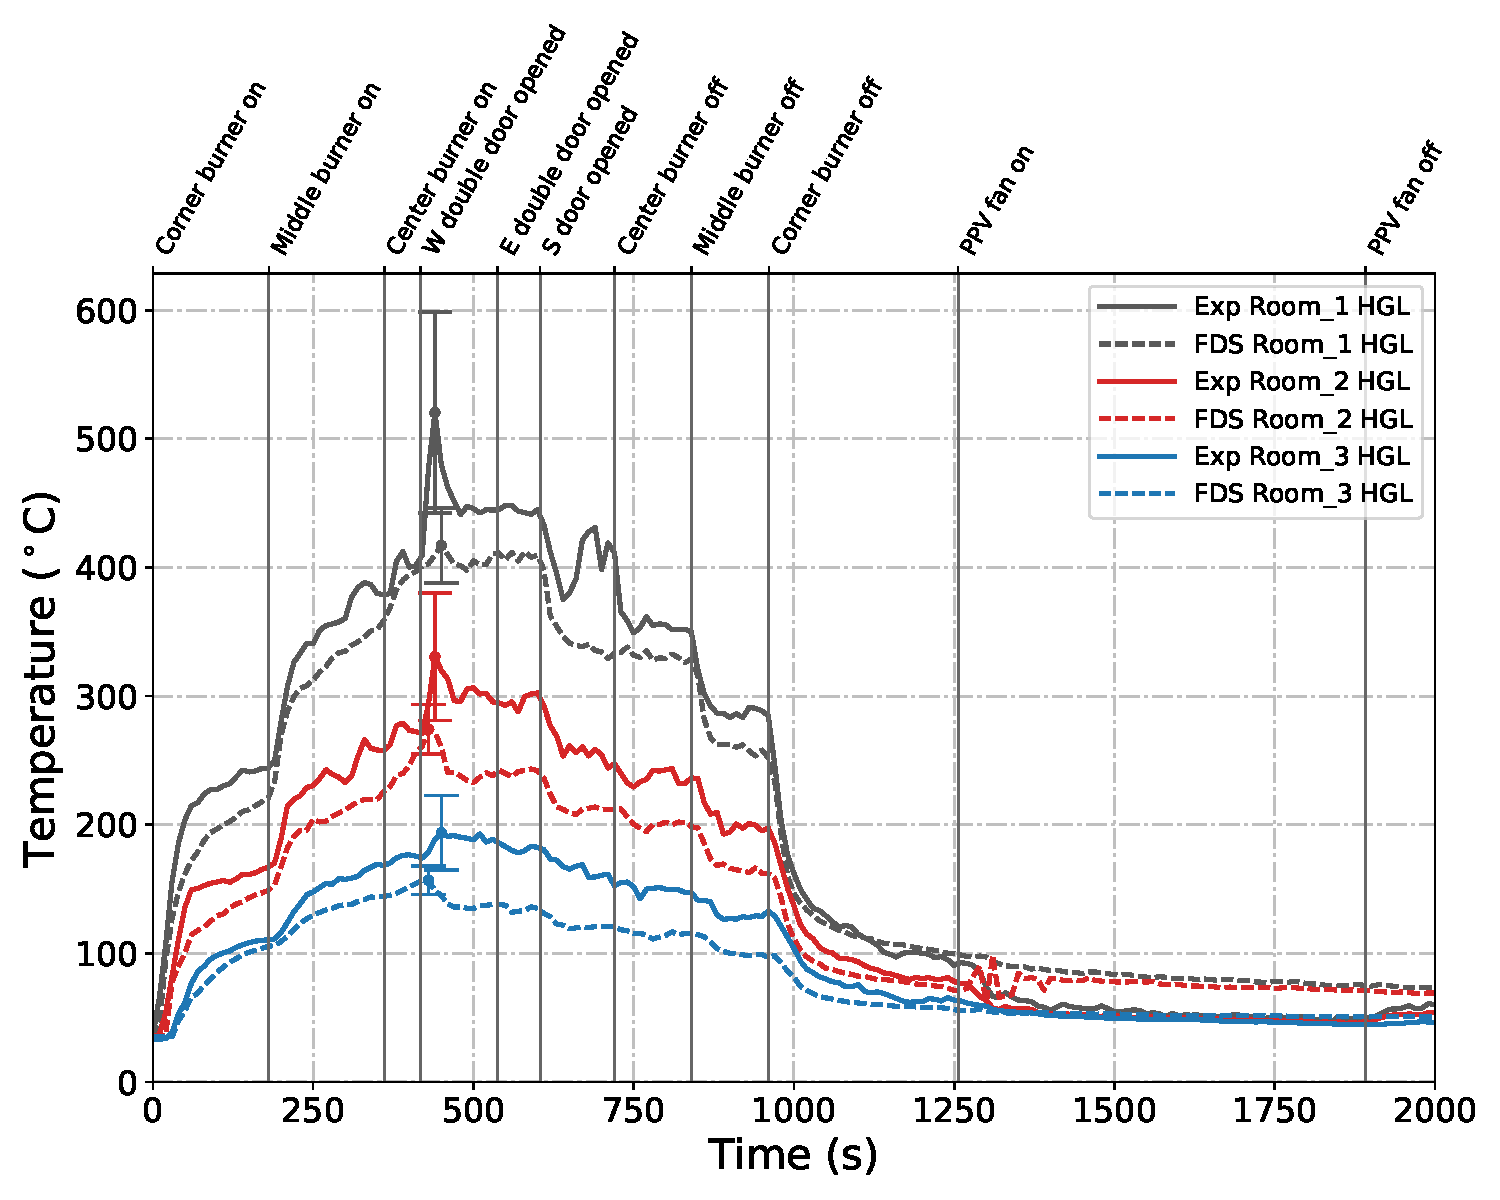
\includegraphics[width=\columnwidth]{Figures/Plots/Validation/Temperature/Test_2_HGL}
	\caption[Plots of measured and predicted hot gas layer temperatures during Test~2.]{Plots of measured and predicted hot gas layer temperatures in the three rooms of the East Structure during Test~2.}
	\label{fig:HGL_data_Test2}
\end{figure}

\begin{figure}[!h]
	\centering
	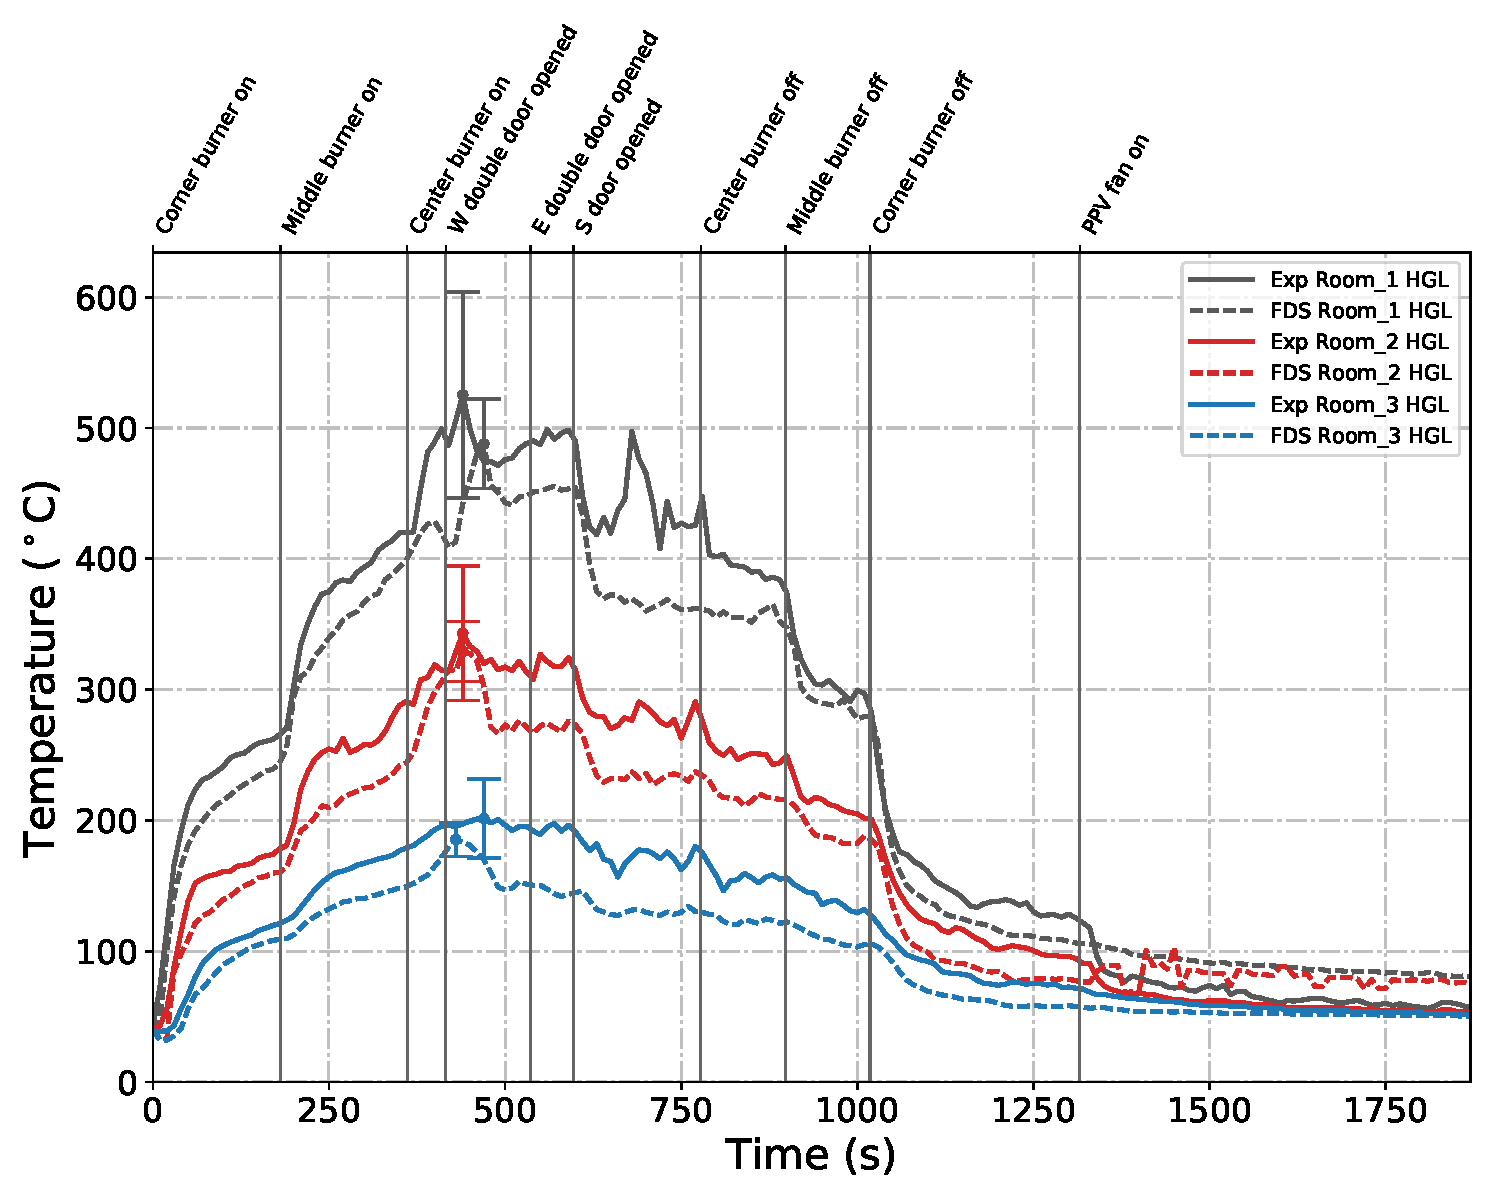
\includegraphics[width=\columnwidth]{Figures/Plots/Validation/Temperature/Test_3_HGL}
	\caption[Plots of measured and predicted hot gas layer temperatures during Test~3.]{Plots of measured and predicted hot gas layer temperatures in the three rooms of the East Structure during Test~3.}
	\label{fig:HGL_data_Test3}
\end{figure}

\begin{figure}[!h]
	\centering
	\includegraphics[width=\columnwidth]{Figures/Plots/Validation/Temperature/Test_4_HGL}
	\caption[Plots of measured and predicted hot gas layer temperatures during Test~4.]{Plots of measured and predicted hot gas layer temperatures in the three rooms of the East Structure during Test~4.}
	\label{fig:HGL_data_Test4}
\end{figure}

\begin{figure}[!h]
	\centering
	\includegraphics[width=\columnwidth]{Figures/Plots/Validation/Temperature/Test_5_HGL}
	\caption[Plots of measured and predicted hot gas layer temperatures during Test~5.]{Plots of measured and predicted hot gas layer temperatures in the three rooms of the East Structure during Test~5.}
	\label{fig:HGL_data_Test5}
\end{figure}

\begin{figure}[!h]
	\centering
	\includegraphics[width=\columnwidth]{Figures/Plots/Validation/Temperature/Test_6_HGL}
	\caption[Plots of measured and predicted hot gas layer temperatures during Test~6.]{Plots of measured and predicted hot gas layer temperatures in the three rooms of the East Structure during Test~6.}
	\label{fig:HGL_data_Test6}
\end{figure}

\begin{figure}[!h]
	\centering
	\includegraphics[width=\columnwidth]{Figures/Plots/Validation/Temperature/Test_23_HGL}
	\caption[Plots of measured and predicted hot gas layer temperatures during Test~23.]{Plots of measured and predicted hot gas layer temperatures on the first and second floors of the West Structure during Test~23.}
	\label{fig:HGL_data_Test23}
\end{figure}

\begin{figure}[!h]
	\centering
	\includegraphics[width=\columnwidth]{Figures/Plots/Validation/Temperature/Test_24_HGL}
	\caption[Plots of measured and predicted hot gas layer temperatures during Test~24.]{Plots of measured and predicted hot gas layer temperatures on the first and second floors of the West Structure during Test~24.}
	\label{fig:HGL_data_Test24}
\end{figure}

\begin{figure}[!h]
	\centering
	\includegraphics[width=\columnwidth]{Figures/Plots/Validation/Temperature/Test_25_HGL}
	\caption[Plots of measured and predicted hot gas layer temperatures during Test~25.]{Plots of measured and predicted hot gas layer temperatures on the first and second floors of the West Structure during Test~25.}
	\label{fig:HGL_data_Test25}
\end{figure}

\clearpage
\subsection*{\textit{Ceiling Jet Temperatures}}
\begin{figure}[!h]
	\centering
	\includegraphics[width=\columnwidth]{Figures/Plots/Validation/Temperature/Test_2_cjet_1}
	\caption[Plots of measured and predicted ceiling jet temperatures during Test~2.]{Plots of measured and predicted ceiling jet temperatures during Test~2 obtained from thermocouple arrays A1, A3, and A5 located in the fire room, middle room, and north room of the East Structure, respectively.}
	\label{fig:cjet1_data_Test2}
\end{figure}

\begin{figure}[!h]
	\centering
	\includegraphics[width=\columnwidth]{Figures/Plots/Validation/Temperature/Test_2_cjet_2}
	\caption[Plots of measured and predicted ceiling jet temperatures during Test~2.]{Plots of measured and predicted ceiling jet temperatures during Test~2 obtained from thermocouple arrays A2 and A4 located in the fire room and north room of the East Structure, respectively.}
	\label{fig:cjet2_data_Test2}
\end{figure}

\begin{figure}[!h]
	\centering
	\includegraphics[width=\columnwidth]{Figures/Plots/Validation/Temperature/Test_3_cjet_1}
	\caption[Plots of measured and predicted ceiling jet temperatures during Test~3.]{Plots of measured and predicted ceiling jet temperatures during Test~3 obtained from thermocouple arrays A1, A3, and A5 located in the fire room, middle room, and north room of the East Structure, respectively.}
	\label{fig:cjet1_data_Test3}
\end{figure}

\begin{figure}[!h]
	\centering
	\includegraphics[width=\columnwidth]{Figures/Plots/Validation/Temperature/Test_3_cjet_2}
	\caption[Plots of measured and predicted ceiling jet temperatures during Test~3.]{Plots of measured and predicted ceiling jet temperatures during Test~3 obtained from thermocouple arrays A2 and A4 located in the fire room and north room of the East Structure, respectively.}
	\label{fig:cjet2_data_Test3}
\end{figure}

\begin{figure}[!h]
	\centering
	\includegraphics[width=\columnwidth]{Figures/Plots/Validation/Temperature/Test_4_cjet_2}
	\caption[Plots of measured and predicted ceiling jet temperatures during Test~4.]{Plots of measured and predicted ceiling jet temperatures during Test~4 obtained from thermocouple arrays A2 and A4 located in the fire room and north room of the East Structure, respectively.}
	\label{fig:cjet2_data_Test4}
\end{figure}

\begin{figure}[!h]
	\centering
	\includegraphics[width=\columnwidth]{Figures/Plots/Validation/Temperature/Test_5_cjet_1}
	\caption[Plots of measured and predicted ceiling jet temperatures during Test~5.]{Plots of measured and predicted ceiling jet temperatures during Test~5 obtained from thermocouple arrays A1, A3, and A5 located in the fire room, middle room, and north room of the East Structure, respectively.}
	\label{fig:cjet1_data_Test5}
\end{figure}

\begin{figure}[!h]
	\centering
	\includegraphics[width=\columnwidth]{Figures/Plots/Validation/Temperature/Test_5_cjet_2}
	\caption[Plots of measured and predicted ceiling jet temperatures during Test~5.]{Plots of measured and predicted ceiling jet temperatures during Test~5 obtained from thermocouple arrays A2 and A4 located in the fire room and north room of the East Structure, respectively.}
	\label{fig:cjet2_data_Test5}
\end{figure}

\begin{figure}[!h]
	\centering
	\includegraphics[width=\columnwidth]{Figures/Plots/Validation/Temperature/Test_6_cjet_1}
	\caption[Plots of measured and predicted ceiling jet temperatures during Test~6.]{Plots of measured and predicted ceiling jet temperatures during Test~6 obtained from thermocouple arrays A1, A3, and A5 located in the fire room, middle room, and north room of the East Structure, respectively.}
	\label{fig:cjet1_data_Test6}
\end{figure}

\begin{figure}[!h]
	\centering
	\includegraphics[width=\columnwidth]{Figures/Plots/Validation/Temperature/Test_6_cjet_2}
	\caption[Plots of measured and predicted ceiling jet temperatures during Test~6.]{Plots of measured and predicted ceiling jet temperatures during Test~6 obtained from thermocouple arrays A2 and A4 located in the fire room and north room of the East Structure, respectively.}
	\label{fig:cjet2_data_Test6}
\end{figure}

\begin{figure}[!h]
	\centering
	\includegraphics[width=\columnwidth]{Figures/Plots/Validation/Temperature/Test_22_cjet_1}
	\caption[Plots of measured and predicted ceiling jet temperatures on the first floor during Test~22.]{Plots of measured and predicted ceiling jet temperatures on the first floor of the West Structure during Test~22.}
	\label{fig:cjet1_data_Test22}
\end{figure}

\begin{figure}[!h]
	\centering
	\includegraphics[width=\columnwidth]{Figures/Plots/Validation/Temperature/Test_22_cjet_2}
	\caption[Plots of measured and predicted ceiling jet temperatures on the second floor during Test~22.]{Plots of measured and predicted ceiling jet temperatures on the second floor of the West Structure during Test~22.}
	\label{fig:cjet2_data_Test22}
\end{figure}

\begin{figure}[!h]
	\centering
	\includegraphics[width=\columnwidth]{Figures/Plots/Validation/Temperature/Test_23_cjet_1}
	\caption[Plots of measured and predicted ceiling jet temperatures on the first floor during Test~23.]{Plots of measured and predicted ceiling jet temperatures on the first floor of the West Structure during Test~23.}
	\label{fig:cjet1_data_Test23}
\end{figure}

\begin{figure}[!h]
	\centering
	\includegraphics[width=\columnwidth]{Figures/Plots/Validation/Temperature/Test_23_cjet_2}
	\caption[Plots of measured and predicted ceiling jet temperatures on the second floor during Test~23.]{Plots of measured and predicted ceiling jet temperatures on the second floor of the West Structure during Test~23.}
	\label{fig:cjet2_data_Test23}
\end{figure}

\begin{figure}[!h]
	\centering
	\includegraphics[width=\columnwidth]{Figures/Plots/Validation/Temperature/Test_24_cjet_1}
	\caption[Plots of measured and predicted ceiling jet temperatures on the first floor during Test~24.]{Plots of measured and predicted ceiling jet temperatures on the first floor of the West Structure during Test~24.}
	\label{fig:cjet1_data_Test24}
\end{figure}

\begin{figure}[!h]
	\centering
	\includegraphics[width=\columnwidth]{Figures/Plots/Validation/Temperature/Test_22_cjet_2}
	\caption[Plots of measured and predicted ceiling jet temperatures on the second floor during Test~24.]{Plots of measured and predicted ceiling jet temperatures on the second floor of the West Structure during Test~24.}
	\label{fig:cjet2_data_Test24}
\end{figure}

\begin{figure}[!h]
	\centering
	\includegraphics[width=\columnwidth]{Figures/Plots/Validation/Temperature/Test_25_cjet_1}
	\caption[Plots of measured and predicted ceiling jet temperatures on the first floor during Test~25.]{Plots of measured and predicted ceiling jet temperatures on the first floor of the West Structure during Test~25.}
	\label{fig:cjet1_data_Test25}
\end{figure}

\begin{figure}[!h]
	\centering
	\includegraphics[width=\columnwidth]{Figures/Plots/Validation/Temperature/Test_25_cjet_2}
	\caption[Plots of measured and predicted ceiling jet temperatures on the second floor during Test~25.]{Plots of measured and predicted ceiling jet temperatures on the second floor of the West Structure during Test~25.}
	\label{fig:cjet2_data_Test25}
\end{figure}

\clearpage
\subsection*{\textit{Thermocouple Array Temperatures}}

\begin{figure}[!h]
	\centering
	\includegraphics[width=\columnwidth]{Figures/Plots/Validation/Temperature/Test_2_TC_A1_upper}
	\caption{Plots of measured and predicted ``upper'' temperatures at array A1 during Test~2 in the East Structure.}
	\label{fig:TCA1_upper_data_Test2}
\end{figure}
\clearpage
\begin{figure}[!h]
	\centering
	\includegraphics[width=\columnwidth]{Figures/Plots/Validation/Temperature/Test_2_TC_A1_lower}
	\caption{Plots of measured and predicted ``lower'' temperatures at array A1 during Test~2 in the East Structure.}
	\label{fig:TCA1_lower_data_Test2}
\end{figure}

\clearpage 

\begin{figure}[!h]
	\centering
	\includegraphics[width=\columnwidth]{Figures/Plots/Validation/Temperature/Test_2_TC_A2_upper}
	\caption{Plots of measured and predicted ``upper'' temperatures at array A2 during Test~2 in the East Structure.}
	\label{fig:TCA2_upper_data_Test2}
\end{figure}

\begin{figure}[!h]
	\centering
	\includegraphics[width=\columnwidth]{Figures/Plots/Validation/Temperature/Test_2_TC_A2_lower}
	\caption{Plots of measured and predicted ``lower'' temperatures at array A2 during Test~2 in the East Structure.}
	\label{fig:TCA2_lower_data_Test2}
\end{figure}

% \begin{figure}[!h]
% 	\centering
% 	\includegraphics[width=\columnwidth]{Figures/Plots/Validation/Temperature/Test_2_TC_A3_upper}
% 	\caption{Plots of measured and predicted ``upper'' temperatures at array A3 during Test~2 in the East Structure.}
% 	\label{fig:TCA3_upper_data_Test2}
% \end{figure}

% \begin{figure}[!h]
% 	\centering
% 	\includegraphics[width=\columnwidth]{Figures/Plots/Validation/Temperature/Test_2_TC_A3_lower}
% 	\caption{Plots of measured and predicted ``lower'' temperatures at array A3 during Test~2 in the East Structure.}
% 	\label{fig:TCA3_lower_data_Test2}
% \end{figure}

% \begin{figure}[!h]
% 	\centering
% 	\includegraphics[width=\columnwidth]{Figures/Plots/Validation/Temperature/Test_2_TC_A4_upper}
% 	\caption{Plots of measured and predicted ``upper'' temperatures at array A4 during Test~2 in the East Structure.}
% 	\label{fig:TCA4_upper_data_Test2}
% \end{figure}

% \begin{figure}[!h]
% 	\centering
% 	\includegraphics[width=\columnwidth]{Figures/Plots/Validation/Temperature/Test_2_TC_A4_lower}
% 	\caption{Plots of measured and predicted ``lower'' temperatures at array A4 during Test~2 in the East Structure.}
% 	\label{fig:TCA4_lower_data_Test2}
% \end{figure}

% \begin{figure}[!h]
% 	\centering
% 	\includegraphics[width=\columnwidth]{Figures/Plots/Validation/Temperature/Test_2_TC_A5_upper}
% 	\caption{Plots of measured and predicted ``upper'' temperatures at array A5 during Test~2 in the East Structure.}
% 	\label{fig:TCA5_upper_data_Test2}
% \end{figure}

% \begin{figure}[!h]
% 	\centering
% 	\includegraphics[width=\columnwidth]{Figures/Plots/Validation/Temperature/Test_2_TC_A5_lower}
% 	\caption{Plots of measured and predicted ``lower'' temperatures at array A5 during Test~2 in the East Structure.}
% 	\label{fig:TCA5_lower_data_Test2}
% \end{figure}

% \begin{figure}[!h]
% 	\centering
% 	\includegraphics[width=\columnwidth]{Figures/Plots/Validation/Temperature/Test_2_TC_A5_upper}
% 	\caption{Plots of measured and predicted ``upper'' temperatures at array A5 during Test~2 in the East Structure.}
% 	\label{fig:TCA5_upper_data_Test2}
% \end{figure}

% \begin{figure}[!h]
% 	\centering
% 	\includegraphics[width=\columnwidth]{Figures/Plots/Validation/Temperature/Test_2_TC_A5_lower}
% 	\caption{Plots of measured and predicted ``lower'' temperatures at array A5 during Test~2 in the East Structure.}
% 	\label{fig:TCA5_lower_data_Test2}
% \end{figure}

% %%%%%%%%%%%%%%%%%%%%%%%%%%%%%%%%%%%%%%%%
% \begin{figure}[!h]
% 	\centering
% 	\includegraphics[width=\columnwidth]{Figures/Plots/Validation/Temperature/Test_3_TC_A1_upper}
% 	\caption{Plots of measured and predicted ``upper'' temperatures at array A1 during Test~3 in the East Structure.}
% 	\label{fig:TCA1_upper_data_Test3}
% \end{figure}

% \begin{figure}[!h]
% 	\centering
% 	\includegraphics[width=\columnwidth]{Figures/Plots/Validation/Temperature/Test_3_TC_A1_lower}
% 	\caption{Plots of measured and predicted ``lower'' temperatures at array A1 during Test~3 in the East Structure.}
% 	\label{fig:TCA1_lower_data_Test3}
% \end{figure}

% \begin{figure}[!h]
% 	\centering
% 	\includegraphics[width=\columnwidth]{Figures/Plots/Validation/Temperature/Test_3_TC_A2_upper}
% 	\caption{Plots of measured and predicted ``upper'' temperatures at array A2 during Test~3 in the East Structure.}
% 	\label{fig:TCA2_upper_data_Test3}
% \end{figure}

% \begin{figure}[!h]
% 	\centering
% 	\includegraphics[width=\columnwidth]{Figures/Plots/Validation/Temperature/Test_3_TC_A2_lower}
% 	\caption{Plots of measured and predicted ``lower'' temperatures at array A2 during Test~3 in the East Structure.}
% 	\label{fig:TCA2_lower_data_Test3}
% \end{figure}

% \begin{figure}[!h]
% 	\centering
% 	\includegraphics[width=\columnwidth]{Figures/Plots/Validation/Temperature/Test_3_TC_A3_upper}
% 	\caption{Plots of measured and predicted ``upper'' temperatures at array A3 during Test~3 in the East Structure.}
% 	\label{fig:TCA3_upper_data_Test3}
% \end{figure}

% \begin{figure}[!h]
% 	\centering
% 	\includegraphics[width=\columnwidth]{Figures/Plots/Validation/Temperature/Test_3_TC_A3_lower}
% 	\caption{Plots of measured and predicted ``lower'' temperatures at array A3 during Test~3 in the East Structure.}
% 	\label{fig:TCA3_lower_data_Test3}
% \end{figure}

% \begin{figure}[!h]
% 	\centering
% 	\includegraphics[width=\columnwidth]{Figures/Plots/Validation/Temperature/Test_3_TC_A4_upper}
% 	\caption{Plots of measured and predicted ``upper'' temperatures at array A4 during Test~3 in the East Structure.}
% 	\label{fig:TCA4_upper_data_Test3}
% \end{figure}

% \begin{figure}[!h]
% 	\centering
% 	\includegraphics[width=\columnwidth]{Figures/Plots/Validation/Temperature/Test_3_TC_A4_lower}
% 	\caption{Plots of measured and predicted ``lower'' temperatures at array A4 during Test~3 in the East Structure.}
% 	\label{fig:TCA4_lower_data_Test3}
% \end{figure}

% \begin{figure}[!h]
% 	\centering
% 	\includegraphics[width=\columnwidth]{Figures/Plots/Validation/Temperature/Test_3_TC_A5_upper}
% 	\caption{Plots of measured and predicted ``upper'' temperatures at array A5 during Test~3 in the East Structure.}
% 	\label{fig:TCA5_upper_data_Test3}
% \end{figure}

% \begin{figure}[!h]
% 	\centering
% 	\includegraphics[width=\columnwidth]{Figures/Plots/Validation/Temperature/Test_3_TC_A5_lower}
% 	\caption{Plots of measured and predicted ``lower'' temperatures at array A5 during Test~3 in the East Structure.}
% 	\label{fig:TCA5_lower_data_Test3}
% \end{figure}

% %%%%%%%%%%%%%%%%%%%%%%%%%%%%%%%%%%%%%%%%
% \begin{figure}[!h]
% 	\centering
% 	\includegraphics[width=\columnwidth]{Figures/Plots/Validation/Temperature/Test_3_TC_A1_upper}
% 	\caption{Plots of measured and predicted ``upper'' temperatures at array A1 during Test~3 in the East Structure.}
% 	\label{fig:TCA1_upper_data_Test3}
% \end{figure}

% \begin{figure}[!h]
% 	\centering
% 	\includegraphics[width=\columnwidth]{Figures/Plots/Validation/Temperature/Test_3_TC_A1_lower}
% 	\caption{Plots of measured and predicted ``lower'' temperatures at array A1 during Test~3 in the East Structure.}
% 	\label{fig:TCA1_lower_data_Test3}
% \end{figure}

% \begin{figure}[!h]
% 	\centering
% 	\includegraphics[width=\columnwidth]{Figures/Plots/Validation/Temperature/Test_3_TC_A2_upper}
% 	\caption{Plots of measured and predicted ``upper'' temperatures at array A2 during Test~3 in the East Structure.}
% 	\label{fig:TCA2_upper_data_Test3}
% \end{figure}

% \begin{figure}[!h]
% 	\centering
% 	\includegraphics[width=\columnwidth]{Figures/Plots/Validation/Temperature/Test_3_TC_A2_lower}
% 	\caption{Plots of measured and predicted ``lower'' temperatures at array A2 during Test~3 in the East Structure.}
% 	\label{fig:TCA2_lower_data_Test3}
% \end{figure}

% \begin{figure}[!h]
% 	\centering
% 	\includegraphics[width=\columnwidth]{Figures/Plots/Validation/Temperature/Test_3_TC_A3_upper}
% 	\caption{Plots of measured and predicted ``upper'' temperatures at array A3 during Test~3 in the East Structure.}
% 	\label{fig:TCA3_upper_data_Test3}
% \end{figure}

% \begin{figure}[!h]
% 	\centering
% 	\includegraphics[width=\columnwidth]{Figures/Plots/Validation/Temperature/Test_3_TC_A3_lower}
% 	\caption{Plots of measured and predicted ``lower'' temperatures at array A3 during Test~3 in the East Structure.}
% 	\label{fig:TCA3_lower_data_Test3}
% \end{figure}

% \begin{figure}[!h]
% 	\centering
% 	\includegraphics[width=\columnwidth]{Figures/Plots/Validation/Temperature/Test_3_TC_A4_upper}
% 	\caption{Plots of measured and predicted ``upper'' temperatures at array A4 during Test~3 in the East Structure.}
% 	\label{fig:TCA4_upper_data_Test3}
% \end{figure}

% \begin{figure}[!h]
% 	\centering
% 	\includegraphics[width=\columnwidth]{Figures/Plots/Validation/Temperature/Test_3_TC_A4_lower}
% 	\caption{Plots of measured and predicted ``lower'' temperatures at array A4 during Test~3 in the East Structure.}
% 	\label{fig:TCA4_lower_data_Test3}
% \end{figure}

% \begin{figure}[!h]
% 	\centering
% 	\includegraphics[width=\columnwidth]{Figures/Plots/Validation/Temperature/Test_3_TC_A5_upper}
% 	\caption{Plots of measured and predicted ``upper'' temperatures at array A5 during Test~3 in the East Structure.}
% 	\label{fig:TCA5_upper_data_Test3}
% \end{figure}

% \begin{figure}[!h]
% 	\centering
% 	\includegraphics[width=\columnwidth]{Figures/Plots/Validation/Temperature/Test_3_TC_A5_lower}
% 	\caption{Plots of measured and predicted ``lower'' temperatures at array A5 during Test~3 in the East Structure.}
% 	\label{fig:TCA5_lower_data_Test3}
% \end{figure}

% %%%%%%%%%%%%%%%%%%%%%%%%%%%%%%%%%%%%%%%%
% \begin{figure}[!h]
% 	\centering
% 	\includegraphics[width=\columnwidth]{Figures/Plots/Validation/Temperature/Test_5_TC_A1_upper}
% 	\caption{Plots of measured and predicted ``upper'' temperatures at array A1 during Test~5 in the East Structure.}
% 	\label{fig:TCA1_upper_data_Test5}
% \end{figure}

% \begin{figure}[!h]
% 	\centering
% 	\includegraphics[width=\columnwidth]{Figures/Plots/Validation/Temperature/Test_5_TC_A1_lower}
% 	\caption{Plots of measured and predicted ``lower'' temperatures at array A1 during Test~5 in the East Structure.}
% 	\label{fig:TCA1_lower_data_Test5}
% \end{figure}

% \begin{figure}[!h]
% 	\centering
% 	\includegraphics[width=\columnwidth]{Figures/Plots/Validation/Temperature/Test_5_TC_A2_upper}
% 	\caption{Plots of measured and predicted ``upper'' temperatures at array A2 during Test~5 in the East Structure.}
% 	\label{fig:TCA2_upper_data_Test5}
% \end{figure}

% \begin{figure}[!h]
% 	\centering
% 	\includegraphics[width=\columnwidth]{Figures/Plots/Validation/Temperature/Test_5_TC_A2_lower}
% 	\caption{Plots of measured and predicted ``lower'' temperatures at array A2 during Test~5 in the East Structure.}
% 	\label{fig:TCA2_lower_data_Test5}
% \end{figure}

% \begin{figure}[!h]
% 	\centering
% 	\includegraphics[width=\columnwidth]{Figures/Plots/Validation/Temperature/Test_5_TC_A3_upper}
% 	\caption{Plots of measured and predicted ``upper'' temperatures at array A3 during Test~5 in the East Structure.}
% 	\label{fig:TCA3_upper_data_Test5}
% \end{figure}

% \begin{figure}[!h]
% 	\centering
% 	\includegraphics[width=\columnwidth]{Figures/Plots/Validation/Temperature/Test_5_TC_A3_lower}
% 	\caption{Plots of measured and predicted ``lower'' temperatures at array A3 during Test~5 in the East Structure.}
% 	\label{fig:TCA3_lower_data_Test5}
% \end{figure}

% \begin{figure}[!h]
% 	\centering
% 	\includegraphics[width=\columnwidth]{Figures/Plots/Validation/Temperature/Test_5_TC_A4_upper}
% 	\caption{Plots of measured and predicted ``upper'' temperatures at array A4 during Test~5 in the East Structure.}
% 	\label{fig:TCA4_upper_data_Test5}
% \end{figure}

% \begin{figure}[!h]
% 	\centering
% 	\includegraphics[width=\columnwidth]{Figures/Plots/Validation/Temperature/Test_5_TC_A4_lower}
% 	\caption{Plots of measured and predicted ``lower'' temperatures at array A4 during Test~5 in the East Structure.}
% 	\label{fig:TCA4_lower_data_Test5}
% \end{figure}

% \begin{figure}[!h]
% 	\centering
% 	\includegraphics[width=\columnwidth]{Figures/Plots/Validation/Temperature/Test_5_TC_A5_upper}
% 	\caption{Plots of measured and predicted ``upper'' temperatures at array A5 during Test~5 in the East Structure.}
% 	\label{fig:TCA5_upper_data_Test5}
% \end{figure}

% \begin{figure}[!h]
% 	\centering
% 	\includegraphics[width=\columnwidth]{Figures/Plots/Validation/Temperature/Test_5_TC_A5_lower}
% 	\caption{Plots of measured and predicted ``lower'' temperatures at array A5 during Test~5 in the East Structure.}
% 	\label{fig:TCA5_lower_data_Test5}
% \end{figure}

% %%%%%%%%%%%%%%%%%%%%%%%%%%%%%%%%%%%%%%%%
% \begin{figure}[!h]
% 	\centering
% 	\includegraphics[width=\columnwidth]{Figures/Plots/Validation/Temperature/Test_3_TC_A1_upper}
% 	\caption{Plots of measured and predicted ``upper'' temperatures at array A1 during Test~3 in the East Structure.}
% 	\label{fig:TCA1_upper_data_Test3}
% \end{figure}

% \begin{figure}[!h]
% 	\centering
% 	\includegraphics[width=\columnwidth]{Figures/Plots/Validation/Temperature/Test_3_TC_A1_lower}
% 	\caption{Plots of measured and predicted ``lower'' temperatures at array A1 during Test~3 in the East Structure.}
% 	\label{fig:TCA1_lower_data_Test3}
% \end{figure}

% \begin{figure}[!h]
% 	\centering
% 	\includegraphics[width=\columnwidth]{Figures/Plots/Validation/Temperature/Test_3_TC_A2_upper}
% 	\caption{Plots of measured and predicted ``upper'' temperatures at array A2 during Test~3 in the East Structure.}
% 	\label{fig:TCA2_upper_data_Test3}
% \end{figure}

% \begin{figure}[!h]
% 	\centering
% 	\includegraphics[width=\columnwidth]{Figures/Plots/Validation/Temperature/Test_3_TC_A2_lower}
% 	\caption{Plots of measured and predicted ``lower'' temperatures at array A2 during Test~3 in the East Structure.}
% 	\label{fig:TCA2_lower_data_Test3}
% \end{figure}

% \begin{figure}[!h]
% 	\centering
% 	\includegraphics[width=\columnwidth]{Figures/Plots/Validation/Temperature/Test_3_TC_A3_upper}
% 	\caption{Plots of measured and predicted ``upper'' temperatures at array A3 during Test~3 in the East Structure.}
% 	\label{fig:TCA3_upper_data_Test3}
% \end{figure}

% \begin{figure}[!h]
% 	\centering
% 	\includegraphics[width=\columnwidth]{Figures/Plots/Validation/Temperature/Test_3_TC_A3_lower}
% 	\caption{Plots of measured and predicted ``lower'' temperatures at array A3 during Test~3 in the East Structure.}
% 	\label{fig:TCA3_lower_data_Test3}
% \end{figure}

% \begin{figure}[!h]
% 	\centering
% 	\includegraphics[width=\columnwidth]{Figures/Plots/Validation/Temperature/Test_3_TC_A4_upper}
% 	\caption{Plots of measured and predicted ``upper'' temperatures at array A4 during Test~3 in the East Structure.}
% 	\label{fig:TCA4_upper_data_Test3}
% \end{figure}

% \begin{figure}[!h]
% 	\centering
% 	\includegraphics[width=\columnwidth]{Figures/Plots/Validation/Temperature/Test_3_TC_A4_lower}
% 	\caption{Plots of measured and predicted ``lower'' temperatures at array A4 during Test~3 in the East Structure.}
% 	\label{fig:TCA4_lower_data_Test3}
% \end{figure}

% \begin{figure}[!h]
% 	\centering
% 	\includegraphics[width=\columnwidth]{Figures/Plots/Validation/Temperature/Test_3_TC_A5_upper}
% 	\caption{Plots of measured and predicted ``upper'' temperatures at array A5 during Test~3 in the East Structure.}
% 	\label{fig:TCA5_upper_data_Test3}
% \end{figure}

% \begin{figure}[!h]
% 	\centering
% 	\includegraphics[width=\columnwidth]{Figures/Plots/Validation/Temperature/Test_3_TC_A5_lower}
% 	\caption{Plots of measured and predicted ``lower'' temperatures at array A5 during Test~3 in the East Structure.}
% 	\label{fig:TCA5_lower_data_Test3}
% \end{figure}

% %%%%%%%%%%%%%%%%%%%%%%%%%%%%%%%%%%%%%%%%
% \begin{figure}[!h]
% 	\centering
% 	\includegraphics[width=\columnwidth]{Figures/Plots/Validation/Temperature/Test_6_TC_A1_upper}
% 	\caption{Plots of measured and predicted ``upper'' temperatures at array A1 during Test~6 in the East Structure.}
% 	\label{fig:TCA1_upper_data_Test6}
% \end{figure}

% \begin{figure}[!h]
% 	\centering
% 	\includegraphics[width=\columnwidth]{Figures/Plots/Validation/Temperature/Test_6_TC_A1_lower}
% 	\caption{Plots of measured and predicted ``lower'' temperatures at array A1 during Test~6 in the East Structure.}
% 	\label{fig:TCA1_lower_data_Test6}
% \end{figure}

% \begin{figure}[!h]
% 	\centering
% 	\includegraphics[width=\columnwidth]{Figures/Plots/Validation/Temperature/Test_6_TC_A2_upper}
% 	\caption{Plots of measured and predicted ``upper'' temperatures at array A2 during Test~6 in the East Structure.}
% 	\label{fig:TCA2_upper_data_Test6}
% \end{figure}

% \begin{figure}[!h]
% 	\centering
% 	\includegraphics[width=\columnwidth]{Figures/Plots/Validation/Temperature/Test_6_TC_A2_lower}
% 	\caption{Plots of measured and predicted ``lower'' temperatures at array A2 during Test~6 in the East Structure.}
% 	\label{fig:TCA2_lower_data_Test6}
% \end{figure}

% \begin{figure}[!h]
% 	\centering
% 	\includegraphics[width=\columnwidth]{Figures/Plots/Validation/Temperature/Test_6_TC_A3_upper}
% 	\caption{Plots of measured and predicted ``upper'' temperatures at array A3 during Test~6 in the East Structure.}
% 	\label{fig:TCA3_upper_data_Test6}
% \end{figure}

% \begin{figure}[!h]
% 	\centering
% 	\includegraphics[width=\columnwidth]{Figures/Plots/Validation/Temperature/Test_6_TC_A3_lower}
% 	\caption{Plots of measured and predicted ``lower'' temperatures at array A3 during Test~6 in the East Structure.}
% 	\label{fig:TCA3_lower_data_Test6}
% \end{figure}

% \begin{figure}[!h]
% 	\centering
% 	\includegraphics[width=\columnwidth]{Figures/Plots/Validation/Temperature/Test_6_TC_A4_upper}
% 	\caption{Plots of measured and predicted ``upper'' temperatures at array A4 during Test~6 in the East Structure.}
% 	\label{fig:TCA4_upper_data_Test6}
% \end{figure}

% \begin{figure}[!h]
% 	\centering
% 	\includegraphics[width=\columnwidth]{Figures/Plots/Validation/Temperature/Test_6_TC_A4_lower}
% 	\caption{Plots of measured and predicted ``lower'' temperatures at array A4 during Test~6 in the East Structure.}
% 	\label{fig:TCA4_lower_data_Test6}
% \end{figure}

% \begin{figure}[!h]
% 	\centering
% 	\includegraphics[width=\columnwidth]{Figures/Plots/Validation/Temperature/Test_6_TC_A5_upper}
% 	\caption{Plots of measured and predicted ``upper'' temperatures at array A5 during Test~6 in the East Structure.}
% 	\label{fig:TCA5_upper_data_Test6}
% \end{figure}

% \begin{figure}[!h]
% 	\centering
% 	\includegraphics[width=\columnwidth]{Figures/Plots/Validation/Temperature/Test_6_TC_A5_lower}
% 	\caption{Plots of measured and predicted ``lower'' temperatures at array A5 during Test~6 in the East Structure.}
% 	\label{fig:TCA5_lower_data_Test6}
% \end{figure}

%%%%%%%%%%%%%%%%%%%%%%%%%%%%%%%%%%%%%%%%
%%%%%%%%%% WEST STRUCTURE %%%%%%%%%%%%%%
%%%%%%%%%%%%%%%%%%%%%%%%%%%%%%%%%%%%%%%%
\begin{figure}[!h]
	\centering
	\includegraphics[width=\columnwidth]{Figures/Plots/Validation/Temperature/Test_22_TC_A1_upper}
	\caption{Plots of measured and predicted ``upper'' temperatures at array A1 during Test~22 in the West Structure.}
	\label{fig:TCA1_upper_data_Test22}
\end{figure}

\begin{figure}[!h]
	\centering
	\includegraphics[width=\columnwidth]{Figures/Plots/Validation/Temperature/Test_22_TC_A1_lower}
	\caption{Plots of measured and predicted ``lower'' temperatures at array A1 during Test~22 in the West Structure.}
	\label{fig:TCA1_lower_data_Test22}
\end{figure}

\begin{figure}[!h]
	\centering
	\includegraphics[width=\columnwidth]{Figures/Plots/Validation/Temperature/Test_22_TC_A2_upper}
	\caption{Plots of measured and predicted ``upper'' temperatures at array A2 during Test~22 in the West Structure.}
	\label{fig:TCA2_upper_data_Test22}
\end{figure}

\begin{figure}[!h]
	\centering
	\includegraphics[width=\columnwidth]{Figures/Plots/Validation/Temperature/Test_22_TC_A2_lower}
	\caption{Plots of measured and predicted ``lower'' temperatures at array A2 during Test~22 in the West Structure.}
	\label{fig:TCA2_lower_data_Test22}
\end{figure}

\begin{figure}[!h]
	\centering
	\includegraphics[width=\columnwidth]{Figures/Plots/Validation/Temperature/Test_22_TC_A3_upper}
	\caption{Plots of measured and predicted ``upper'' temperatures at array A3 during Test~22 in the West Structure.}
	\label{fig:TCA3_upper_data_Test22}
\end{figure}

\begin{figure}[!h]
	\centering
	\includegraphics[width=\columnwidth]{Figures/Plots/Validation/Temperature/Test_22_TC_A3_lower}
	\caption{Plots of measured and predicted ``lower'' temperatures at array A3 during Test~22 in the West Structure.}
	\label{fig:TCA3_lower_data_Test22}
\end{figure}

\begin{figure}[!h]
	\centering
	\includegraphics[width=\columnwidth]{Figures/Plots/Validation/Temperature/Test_22_TC_A7_upper}
	\caption{Plots of measured and predicted ``upper'' temperatures at array A7 during Test~22 in the West Structure.}
	\label{fig:TCA7_upper_data_Test22}
\end{figure}

\begin{figure}[!h]
	\centering
	\includegraphics[width=\columnwidth]{Figures/Plots/Validation/Temperature/Test_22_TC_A7_lower}
	\caption{Plots of measured and predicted ``lower'' temperatures at array A7 during Test~22 in the West Structure.}
	\label{fig:TCA7_lower_data_Test22}
\end{figure}

\begin{figure}[!h]
	\centering
	\includegraphics[width=\columnwidth]{Figures/Plots/Validation/Temperature/Test_22_TC_A8_upper}
	\caption{Plots of measured and predicted ``upper'' temperatures at array A8 during Test~22 in the West Structure.}
	\label{fig:TCA8_upper_data_Test22}
\end{figure}

\begin{figure}[!h]
	\centering
	\includegraphics[width=\columnwidth]{Figures/Plots/Validation/Temperature/Test_22_TC_A8_lower}
	\caption{Plots of measured and predicted ``lower'' temperatures at array A8 during Test~22 in the West Structure.}
	\label{fig:TCA8_lower_data_Test22}
\end{figure}

\begin{figure}[!h]
	\centering
	\includegraphics[width=\columnwidth]{Figures/Plots/Validation/Temperature/Test_22_TC_A9_upper}
	\caption{Plots of measured and predicted ``upper'' temperatures at array A9 during Test~22 in the West Structure.}
	\label{fig:TCA9_upper_data_Test22}
\end{figure}

\begin{figure}[!h]
	\centering
	\includegraphics[width=\columnwidth]{Figures/Plots/Validation/Temperature/Test_22_TC_A9_lower}
	\caption{Plots of measured and predicted ``lower'' temperatures at array A9 during Test~22 in the West Structure.}
	\label{fig:TCA9_lower_data_Test22}
\end{figure}

%%%%%%%%%%%%%%%%%%%%%%%%%%%%%%%%%%%%%%%%%%%
\begin{figure}[!h]
	\centering
	\includegraphics[width=\columnwidth]{Figures/Plots/Validation/Temperature/Test_23_TC_A1_upper}
	\caption{Plots of measured and predicted ``upper'' temperatures at array A1 during Test~23 in the West Structure.}
	\label{fig:TCA1_upper_data_Test23}
\end{figure}
\begin{figure}[!h]
	\centering
	\includegraphics[width=\columnwidth]{Figures/Plots/Validation/Temperature/Test_23_TC_A1_lower}
	\caption{Plots of measured and predicted ``lower'' temperatures at array A1 during Test~23 in the West Structure.}
	\label{fig:TCA1_lower_data_Test23}
\end{figure}

\begin{figure}[!h]
	\centering
	\includegraphics[width=\columnwidth]{Figures/Plots/Validation/Temperature/Test_23_TC_A2_upper}
	\caption{Plots of measured and predicted ``upper'' temperatures at array A2 during Test~23 in the West Structure.}
	\label{fig:TCA2_upper_data_Test23}
\end{figure}

\begin{figure}[!h]
	\centering
	\includegraphics[width=\columnwidth]{Figures/Plots/Validation/Temperature/Test_23_TC_A2_lower}
	\caption{Plots of measured and predicted ``lower'' temperatures at array A2 during Test~23 in the West Structure.}
	\label{fig:TCA2_lower_data_Test23}
\end{figure}

\begin{figure}[!h]
	\centering
	\includegraphics[width=\columnwidth]{Figures/Plots/Validation/Temperature/Test_23_TC_A3_upper}
	\caption{Plots of measured and predicted ``upper'' temperatures at array A3 during Test~23 in the West Structure.}
	\label{fig:TCA3_upper_data_Test23}
\end{figure}

\begin{figure}[!h]
	\centering
	\includegraphics[width=\columnwidth]{Figures/Plots/Validation/Temperature/Test_23_TC_A3_lower}
	\caption{Plots of measured and predicted ``lower'' temperatures at array A3 during Test~23 in the West Structure.}
	\label{fig:TCA3_lower_data_Test23}
\end{figure}

\begin{figure}[!h]
	\centering
	\includegraphics[width=\columnwidth]{Figures/Plots/Validation/Temperature/Test_23_TC_A7_upper}
	\caption{Plots of measured and predicted ``upper'' temperatures at array A7 during Test~23 in the West Structure.}
	\label{fig:TCA7_upper_data_Test23}
\end{figure}

\begin{figure}[!h]
	\centering
	\includegraphics[width=\columnwidth]{Figures/Plots/Validation/Temperature/Test_23_TC_A7_lower}
	\caption{Plots of measured and predicted ``lower'' temperatures at array A7 during Test~23 in the West Structure.}
	\label{fig:TCA7_lower_data_Test23}
\end{figure}

\begin{figure}[!h]
	\centering
	\includegraphics[width=\columnwidth]{Figures/Plots/Validation/Temperature/Test_23_TC_A8_upper}
	\caption{Plots of measured and predicted ``upper'' temperatures at array A8 during Test~23 in the West Structure.}
	\label{fig:TCA8_upper_data_Test23}
\end{figure}

\begin{figure}[!h]
	\centering
	\includegraphics[width=\columnwidth]{Figures/Plots/Validation/Temperature/Test_23_TC_A8_lower}
	\caption{Plots of measured and predicted ``lower'' temperatures at array A8 during Test~23 in the West Structure.}
	\label{fig:TCA8_lower_data_Test23}
\end{figure}

\begin{figure}[!h]
	\centering
	\includegraphics[width=\columnwidth]{Figures/Plots/Validation/Temperature/Test_23_TC_A9_upper}
	\caption{Plots of measured and predicted ``upper'' temperatures at array A9 during Test~23 in the West Structure.}
	\label{fig:TCA9_upper_data_Test23}
\end{figure}

\begin{figure}[!h]
	\centering
	\includegraphics[width=\columnwidth]{Figures/Plots/Validation/Temperature/Test_23_TC_A9_lower}
	\caption{Plots of measured and predicted ``lower'' temperatures at array A9 during Test~23 in the West Structure.}
	\label{fig:TCA9_lower_data_Test23}
\end{figure}
%%%%%%%%%%%%%%%%%%%%
\begin{figure}[!h]
	\centering
	\includegraphics[width=\columnwidth]{Figures/Plots/Validation/Temperature/Test_24_TC_A1_lower}
	\caption{Plots of measured and predicted ``lower'' temperatures at array A1 during Test~24 in the West Structure.}
	\label{fig:TCA1_lower_data_Test24}
\end{figure}

\begin{figure}[!h]
	\centering
	\includegraphics[width=\columnwidth]{Figures/Plots/Validation/Temperature/Test_24_TC_A2_upper}
	\caption{Plots of measured and predicted ``upper'' temperatures at array A2 during Test~24 in the West Structure.}
	\label{fig:TCA2_upper_data_Test24}
\end{figure}

\begin{figure}[!h]
	\centering
	\includegraphics[width=\columnwidth]{Figures/Plots/Validation/Temperature/Test_24_TC_A2_lower}
	\caption{Plots of measured and predicted ``lower'' temperatures at array A2 during Test~24 in the West Structure.}
	\label{fig:TCA2_lower_data_Test24}
\end{figure}

\begin{figure}[!h]
	\centering
	\includegraphics[width=\columnwidth]{Figures/Plots/Validation/Temperature/Test_24_TC_A3_upper}
	\caption{Plots of measured and predicted ``upper'' temperatures at array A3 during Test~24 in the West Structure.}
	\label{fig:TCA3_upper_data_Test24}
\end{figure}

\begin{figure}[!h]
	\centering
	\includegraphics[width=\columnwidth]{Figures/Plots/Validation/Temperature/Test_24_TC_A3_lower}
	\caption{Plots of measured and predicted ``lower'' temperatures at array A3 during Test~24 in the West Structure.}
	\label{fig:TCA3_lower_data_Test24}
\end{figure}

\begin{figure}[!h]
	\centering
	\includegraphics[width=\columnwidth]{Figures/Plots/Validation/Temperature/Test_24_TC_A7_upper}
	\caption{Plots of measured and predicted ``upper'' temperatures at array A7 during Test~24 in the West Structure.}
	\label{fig:TCA7_upper_data_Test24}
\end{figure}

\begin{figure}[!h]
	\centering
	\includegraphics[width=\columnwidth]{Figures/Plots/Validation/Temperature/Test_24_TC_A7_lower}
	\caption{Plots of measured and predicted ``lower'' temperatures at array A7 during Test~24 in the West Structure.}
	\label{fig:TCA7_lower_data_Test24}
\end{figure}

\begin{figure}[!h]
	\centering
	\includegraphics[width=\columnwidth]{Figures/Plots/Validation/Temperature/Test_24_TC_A8_upper}
	\caption{Plots of measured and predicted ``upper'' temperatures at array A8 during Test~24 in the West Structure.}
	\label{fig:TCA8_upper_data_Test24}
\end{figure}

\begin{figure}[!h]
	\centering
	\includegraphics[width=\columnwidth]{Figures/Plots/Validation/Temperature/Test_24_TC_A8_lower}
	\caption{Plots of measured and predicted ``lower'' temperatures at array A8 during Test~24 in the West Structure.}
	\label{fig:TCA8_lower_data_Test24}
\end{figure}

\begin{figure}[!h]
	\centering
	\includegraphics[width=\columnwidth]{Figures/Plots/Validation/Temperature/Test_24_TC_A9_upper}
	\caption{Plots of measured and predicted ``upper'' temperatures at array A9 during Test~24 in the West Structure.}
	\label{fig:TCA9_upper_data_Test24}
\end{figure}

\begin{figure}[!h]
	\centering
	\includegraphics[width=\columnwidth]{Figures/Plots/Validation/Temperature/Test_24_TC_A9_lower}
	\caption{Plots of measured and predicted ``lower'' temperatures at array A9 during Test~24 in the West Structure.}
	\label{fig:TCA9_lower_data_Test24}
\end{figure}
%%%%%%%%%%%%%%%%%%%%%%%%%%%%%%%%%%%%%%%%%%%
\begin{figure}[!h]
	\centering
	\includegraphics[width=\columnwidth]{Figures/Plots/Validation/Temperature/Test_25_TC_A1_upper}
	\caption{Plots of measured and predicted ``upper'' temperatures at array A1 during Test~25 in the West Structure.}
	\label{fig:TCA1_upper_data_Test25}
\end{figure}
\begin{figure}[!h]
	\centering
	\includegraphics[width=\columnwidth]{Figures/Plots/Validation/Temperature/Test_25_TC_A1_lower}
	\caption{Plots of measured and predicted ``lower'' temperatures at array A1 during Test~25 in the West Structure.}
	\label{fig:TCA1_lower_data_Test25}
\end{figure}

\begin{figure}[!h]
	\centering
	\includegraphics[width=\columnwidth]{Figures/Plots/Validation/Temperature/Test_25_TC_A2_upper}
	\caption{Plots of measured and predicted ``upper'' temperatures at array A2 during Test~25 in the West Structure.}
	\label{fig:TCA2_upper_data_Test25}
\end{figure}

\begin{figure}[!h]
	\centering
	\includegraphics[width=\columnwidth]{Figures/Plots/Validation/Temperature/Test_25_TC_A2_lower}
	\caption{Plots of measured and predicted ``lower'' temperatures at array A2 during Test~25 in the West Structure.}
	\label{fig:TCA2_lower_data_Test25}
\end{figure}

\begin{figure}[!h]
	\centering
	\includegraphics[width=\columnwidth]{Figures/Plots/Validation/Temperature/Test_25_TC_A3_upper}
	\caption{Plots of measured and predicted ``upper'' temperatures at array A3 during Test~25 in the West Structure.}
	\label{fig:TCA3_upper_data_Test25}
\end{figure}

\begin{figure}[!h]
	\centering
	\includegraphics[width=\columnwidth]{Figures/Plots/Validation/Temperature/Test_25_TC_A3_lower}
	\caption{Plots of measured and predicted ``lower'' temperatures at array A3 during Test~25 in the West Structure.}
	\label{fig:TCA3_lower_data_Test25}
\end{figure}

\begin{figure}[!h]
	\centering
	\includegraphics[width=\columnwidth]{Figures/Plots/Validation/Temperature/Test_25_TC_A7_upper}
	\caption{Plots of measured and predicted ``upper'' temperatures at array A7 during Test~25 in the West Structure.}
	\label{fig:TCA7_upper_data_Test25}
\end{figure}

\begin{figure}[!h]
	\centering
	\includegraphics[width=\columnwidth]{Figures/Plots/Validation/Temperature/Test_25_TC_A7_lower}
	\caption{Plots of measured and predicted ``lower'' temperatures at array A7 during Test~25 in the West Structure.}
	\label{fig:TCA7_lower_data_Test25}
\end{figure}

\begin{figure}[!h]
	\centering
	\includegraphics[width=\columnwidth]{Figures/Plots/Validation/Temperature/Test_25_TC_A8_upper}
	\caption{Plots of measured and predicted ``upper'' temperatures at array A8 during Test~25 in the West Structure.}
	\label{fig:TCA8_upper_data_Test25}
\end{figure}

\begin{figure}[!h]
	\centering
	\includegraphics[width=\columnwidth]{Figures/Plots/Validation/Temperature/Test_25_TC_A8_lower}
	\caption{Plots of measured and predicted ``lower'' temperatures at array A8 during Test~25 in the West Structure.}
	\label{fig:TCA8_lower_data_Test25}
\end{figure}

\begin{figure}[!h]
	\centering
	\includegraphics[width=\columnwidth]{Figures/Plots/Validation/Temperature/Test_25_TC_A9_upper}
	\caption{Plots of measured and predicted ``upper'' temperatures at array A9 during Test~25 in the West Structure.}
	\label{fig:TCA9_upper_data_Test25}
\end{figure}

\begin{figure}[!h]
	\centering
	\includegraphics[width=\columnwidth]{Figures/Plots/Validation/Temperature/Test_25_TC_A9_lower}
	\caption{Plots of measured and predicted ``lower'' temperatures at array A9 during Test~25 in the West Structure.}
	\label{fig:TCA9_lower_data_Test25}
\end{figure}

\clearpage
\section{Gas Species Concentration}
\subsection*{\textit{O$_2$ Concentration}}
\begin{figure}[!h]
	\centering
	\includegraphics[width=\columnwidth]{Figures/Plots/Validation/Gas_Concentration/Test_2_O2}
	\caption[Plots of measured and predicted $O_2$ concentration during Test~2.]{Plots of measured and predicted $O_2$ concentration in the fire room (black plots) and north room (red plots) of the East Structure during Test~2.}
	\label{fig:Test2_O2}
\end{figure}

\begin{figure}[!h]
	\centering
	\includegraphics[width=\columnwidth]{Figures/Plots/Validation/Gas_Concentration/Test_4_O2}
	\caption[Plots of measured and predicted $O_2$ concentration during Test~4.]{Plots of measured and predicted $O_2$ concentration in the fire room (black plots) and north room (red plots) of the East Structure during Test~4.}
	\label{fig:Test4_O2}
\end{figure}

\begin{figure}[!h]
	\centering
	\includegraphics[width=\columnwidth]{Figures/Plots/Validation/Gas_Concentration/Test_5_O2}
	\caption[Plots of measured and predicted $O_2$ concentration during Test~5.]{Plots of measured and predicted $O_2$ concentration in the fire room (black plots) and north room (red plots) of the East Structure during Test~5.}
	\label{fig:Test5_O2}
\end{figure}

\begin{figure}[!h]
	\centering
	\includegraphics[width=\columnwidth]{Figures/Plots/Validation/Gas_Concentration/Test_6_O2}
	\caption[Plots of measured and predicted $O_2$ concentration during Test~6.]{Plots of measured and predicted $O_2$ concentration in the fire room (black plots) and north room (red plots) of the East Structure during Test~6.}
	\label{fig:Test6_O2}
\end{figure}

\begin{figure}[!h]
	\centering
	\includegraphics[width=\columnwidth]{Figures/Plots/Validation/Gas_Concentration/Test_22_O2}
	\caption[Plots of measured and predicted $O_2$ concentration during Test~22.]{Plots of measured and predicted $O_2$ concentration on the first floor (black plots) and second floor (red plots) of the West Structure during Test~22.}
	\label{fig:Test22_O2}
\end{figure}

\begin{figure}[!h]
	\centering
	\includegraphics[width=\columnwidth]{Figures/Plots/Validation/Gas_Concentration/Test_23_O2}
	\caption[Plots of measured and predicted $O_2$ concentration during Test~23.]{Plots of measured and predicted $O_2$ concentration on the first floor (black plots) and second floor (red plots) of the West Structure during Test~23.}
	\label{fig:Test23_O2}
\end{figure}

\begin{figure}[!h]
	\centering
	\includegraphics[width=\columnwidth]{Figures/Plots/Validation/Gas_Concentration/Test_24_O2}
	\caption[Plots of measured and predicted $O_2$ concentration during Test~24.]{Plots of measured and predicted $O_2$ concentration on the first floor (black plots) and second floor (red plots) of the West Structure during Test~24.}
	\label{fig:Test24_O2}
\end{figure}

\begin{figure}[!h]
	\centering
	\includegraphics[width=\columnwidth]{Figures/Plots/Validation/Gas_Concentration/Test_25_O2}
	\caption[Plots of measured and predicted $O_2$ concentration during Test~25.]{Plots of measured and predicted $O_2$ concentration on the first floor (black plots) and second floor (red plots) of the West Structure during Test~25.}
	\label{fig:Test25_O2}
\end{figure}

\clearpage
\subsection*{\textit{CO$_2$ Concentration}}
\begin{figure}[!h]
	\centering
	\includegraphics[width=\columnwidth]{Figures/Plots/Validation/Gas_Concentration/Test_2_CO2}
	\caption[Plots of measured and predicted $CO_2$ concentration during Test~2.]{Plots of measured and predicted $CO_2$ concentration in the fire room (black plots) and north room (red plots) of the East Structure during Test~2.}
	\label{fig:Test2_CO2}
\end{figure}

\begin{figure}[!h]
	\centering
	\includegraphics[width=\columnwidth]{Figures/Plots/Validation/Gas_Concentration/Test_4_CO2}
	\caption[Plots of measured and predicted $CO_2$ concentration during Test~4.]{Plots of measured and predicted $CO_2$ concentration in the fire room (black plots) and north room (red plots) of the East Structure during Test~4.}
	\label{fig:Test4_CO2}
\end{figure}

\begin{figure}[!h]
	\centering
	\includegraphics[width=\columnwidth]{Figures/Plots/Validation/Gas_Concentration/Test_5_CO2}
	\caption[Plots of measured and predicted $CO_2$ concentration during Test~5.]{Plots of measured and predicted $CO_2$ concentration in the fire room (black plots) and north room (red plots) of the East Structure during Test~5.}
	\label{fig:Test5_CO2}
\end{figure}

\begin{figure}[!h]
	\centering
	\includegraphics[width=\columnwidth]{Figures/Plots/Validation/Gas_Concentration/Test_6_CO2}
	\caption[Plots of measured and predicted $CO_2$ concentration during Test~6.]{Plots of measured and predicted $CO_2$ concentration in the fire room (black plots) and north room (red plots) of the East Structure during Test~6.}
	\label{fig:Test6_CO2}
\end{figure}

\begin{figure}[!h]
	\centering
	\includegraphics[width=\columnwidth]{Figures/Plots/Validation/Gas_Concentration/Test_22_CO2}
	\caption[Plots of measured and predicted $CO_2$ concentration during Test~22.]{Plots of measured and predicted $CO_2$ concentration on the first floor (black plots) and second floor (red plots) of the West Structure during Test~22.}
	\label{fig:Test22_CO2}
\end{figure}

\begin{figure}[!h]
	\centering
	\includegraphics[width=\columnwidth]{Figures/Plots/Validation/Gas_Concentration/Test_23_CO2}
	\caption[Plots of measured and predicted $CO_2$ concentration during Test~23.]{Plots of measured and predicted $CO_2$ concentration on the first floor (black plots) and second floor (red plots) of the West Structure during Test~23.}
	\label{fig:Test23_CO2}
\end{figure}

\begin{figure}[!h]
	\centering
	\includegraphics[width=\columnwidth]{Figures/Plots/Validation/Gas_Concentration/Test_24_CO2}
	\caption[Plots of measured and predicted $CO_2$ concentration during Test~24.]{Plots of measured and predicted $CO_2$ concentration on the first floor (black plots) and second floor (red plots) of the West Structure during Test~24.}
	\label{fig:Test24_CO2}
\end{figure}

\begin{figure}[!h]
	\centering
	\includegraphics[width=\columnwidth]{Figures/Plots/Validation/Gas_Concentration/Test_25_CO2}
	\caption[Plots of measured and predicted $CO_2$ concentration during Test~25.]{Plots of measured and predicted $CO_2$ concentration on the first floor (black plots) and second floor (red plots) of the West Structure during Test~25.}
	\label{fig:Test25_CO2}
\end{figure}

\clearpage
\section{Gas Velocity}
\begin{figure}[!h]
	\centering
	\includegraphics[width=\columnwidth]{Figures/Plots/Validation/Velocity/Test_6_BDP_A10}
	\caption[Plots of measured and predicted gas velocity data at BDP locations in A10 during Test~6.]{Plots of measured and predicted gas velocity data at the BDP locations in array A10 at the East Structure roof vent during Test~6.}
	\label{fig:Test6_BDPs}
\end{figure}

\begin{figure}[!h]
	\centering
	\includegraphics[width=\columnwidth]{Figures/Plots/Validation/Velocity/Test_22_BDP_A10_upper}
	\caption[Plots of measured and predicted gas velocity data at ``upper'' BDP locations in A10 during Test~22.]{Plots of measured and predicted gas velocity data at the ``upper'' BDP locations in array A10 at the stairway door in the West Structure during Test~22.}
	\label{fig:Test22_upper_BDPs}
\end{figure}

\begin{figure}[!h]
	\centering
	\includegraphics[width=\columnwidth]{Figures/Plots/Validation/Velocity/Test_22_BDP_A10_lower}
	\caption[Plots of measured and predicted gas velocity data at ``lower'' BDP locations in A10 during Test~22.]{Plots of measured and predicted gas velocity data at the ``lower'' BDP locations in array A10 at the stairway door in the West Structure during Test~22.}
	\label{fig:Test22_lower_BDPs}
\end{figure}

\begin{figure}[!h]
	\centering
	\includegraphics[width=\columnwidth]{Figures/Plots/Validation/Velocity/Test_23_BDP_A10_upper}
	\caption[Plots of measured and predicted gas velocity data at ``upper'' BDP locations in A10 during Test~23.]{Plots of measured and predicted gas velocity data at the ``upper'' BDP locations in array A10 at the stairway door in the West Structure during Test~23.}
	\label{fig:Test23_upper_BDPs}
\end{figure}

\begin{figure}[!h]
	\centering
	\includegraphics[width=\columnwidth]{Figures/Plots/Validation/Velocity/Test_23_BDP_A10_lower}
	\caption[Plots of measured and predicted gas velocity data at ``lower'' BDP locations in A10 during Test~23.]{Plots of measured and predicted gas velocity data at the ``lower'' BDP locations in array A10 at the stairway door in the West Structure during Test~23.}
	\label{fig:Test23_lower_BDPs}
\end{figure}

\begin{figure}[!h]
	\centering
	\includegraphics[width=\columnwidth]{Figures/Plots/Validation/Velocity/Test_24_BDP_A10_upper}
	\caption[Plots of measured and predicted gas velocity data at ``upper'' BDP locations in A10 during Test~24.]{Plots of measured and predicted gas velocity data at the ``upper'' BDP locations in array A10 at the stairway door in the West Structure during Test~24.}
	\label{fig:Test24_upper_BDPs}
\end{figure}

\begin{figure}[!h]
	\centering
	\includegraphics[width=\columnwidth]{Figures/Plots/Validation/Velocity/Test_24_BDP_A10_lower}
	\caption[Plots of measured and predicted gas velocity data at ``lower'' BDP locations in A10 during Test~24.]{Plots of measured and predicted gas velocity data at the ``lower'' BDP locations in array A10 at the stairway door in the West Structure during Test~24.}
	\label{fig:Test24_lower_BDPs}
\end{figure}

\begin{figure}[!h]
	\centering
	\includegraphics[width=\columnwidth]{Figures/Plots/Validation/Velocity/Test_25_BDP_A10_upper}
	\caption[Plots of measured and predicted gas velocity data at ``upper'' BDP locations in A10 during Test~25.]{Plots of measured and predicted gas velocity data at the ``upper'' BDP locations in array A10 at the stairway door in the West Structure during Test~25.}
	\label{fig:Test25_upper_BDPs}
\end{figure}

\begin{figure}[!h]
	\centering
	\includegraphics[width=\columnwidth]{Figures/Plots/Validation/Velocity/Test_25_BDP_A10_lower}
	\caption[Plots of measured and predicted gas velocity data at ``lower'' BDP locations in A10 during Test~25.]{Plots of measured and predicted gas velocity data at the ``lower'' BDP locations in array A10 at the stairway door in the West Structure during Test~25.}
	\label{fig:Test25_lower_BDPs}
\end{figure}

\clearpage
\section{Total Heat Flux}

\begin{figure}[!h]
	\centering
	\includegraphics[width=\columnwidth]{Figures/Plots/Validation/Heat_Flux/Test_2_HFs}
	\caption[Plots of measured and predicted heat flux data during Test~2.]{Plots of measured and predicted heat flux data at the gauge locations in the fire room (A1), the center room (A3) and the north room (A4 and A5) of the East Structure during Test~2.}
	\label{fig:Test2_HFs}
\end{figure}

\begin{figure}[!h]
	\centering
	\includegraphics[width=\columnwidth]{Figures/Plots/Validation/Heat_Flux/Test_3_HFs}
	\caption[Plots of measured and predicted heat flux data during Test~3.]{Plots of measured and predicted heat flux data at the gauge locations in the fire room (A1), the center room (A3) and the north room (A4 and A5) of the East Structure during Test~3.}
	\label{fig:Test3_HFs}
\end{figure}

\begin{figure}[!h]
	\centering
	\includegraphics[width=\columnwidth]{Figures/Plots/Validation/Heat_Flux/Test_4_HFs}
	\caption[Plots of measured and predicted heat flux data during Test~4.]{Plots of measured and predicted heat flux data at the gauge locations in the fire room (A1), the center room (A3) and the north room (A4 and A5) of the East Structure during Test~4.}
	\label{fig:Test4_HFs}
\end{figure}

\begin{figure}[!h]
	\centering
	\includegraphics[width=\columnwidth]{Figures/Plots/Validation/Heat_Flux/Test_5_HFs}
	\caption[Plots of measured and predicted heat flux data during Test~5.]{Plots of measured and predicted heat flux data at the gauge locations in the fire room (A1), the center room (A3) and the north room (A4 and A5) of the East Structure during Test~5.}
	\label{fig:Test5_HFs}
\end{figure}

\begin{figure}[!h]
	\centering
	\includegraphics[width=\columnwidth]{Figures/Plots/Validation/Heat_Flux/Test_6_HFs}
	\caption[Plots of measured and predicted heat flux data during Test~6.]{Plots of measured and predicted heat flux data at the gauge locations in the fire room (A1), the center room (A3) and the north room (A4 and A5) of the East Structure during Test~6.}
	\label{fig:Test6_HFs}
\end{figure}

\begin{figure}[!h]
	\centering
	\includegraphics[width=\columnwidth]{Figures/Plots/Validation/Heat_Flux/Test_22_HFs}
	\caption[Plots of measured and predicted heat flux data during Test~22.]{Plots of measured and predicted heat flux data at the locations near the stairway door and near the south door on the second floor of the West Structure during Test~22.}
	\label{fig:Test22_HFs}
\end{figure}

\begin{figure}[!h]
	\centering
	\includegraphics[width=\columnwidth]{Figures/Plots/Validation/Heat_Flux/Test_24_HFs}
	\caption[Plots of measured and predicted heat flux data during Test~24.]{Plots of measured and predicted heat flux data at the locations near the stairway door and near the south door on the second floor of the West Structure during Test~24.}
	\label{fig:Test24_HFs}
\end{figure}

\begin{figure}[!h]
	\centering
	\includegraphics[width=\columnwidth]{Figures/Plots/Validation/Heat_Flux/Test_25_HFs}
	\caption[Plots of measured and predicted heat flux data during Test~25.]{Plots of measured and predicted heat flux data at the locations near the stairway door and near the south door on the second floor of the West Structure during Test~25.}
	\label{fig:Test25_HFs}
\end{figure}


\renewcommand{\baselinestretch}{1}
\small\normalsize

\newpage
\bibliographystyle{unsrt}
\bibliography{../Bibliography/FDS_refs,../Bibliography/FDS_general}

\end{document}
